
\documentclass[12pt]{report}
\usepackage{jrl_thesis}
\usepackage{fancyheadings}
\usepackage{natbib}
\usepackage{setspace}               % this package defines the spacing of your thesis and should be included
             % your information goes here
\usepackage{titlesec}
\usepackage{hyperref}
\usepackage[pdftex]{graphicx}
\usepackage{subcaption}
\usepackage{mathtools}
\usepackage{amsmath}
\usepackage{caption}
\usepackage{verbatim}
\usepackage{cleveref}
\usepackage{listings}
\usepackage[per-mode = symbol]{siunitx}
\usepackage{amssymb} 
\usepackage{mathrsfs}
\usepackage{float}
\usepackage{rotating}

%\usepackage[framed,numbered,autolinebreaks,useliterate]{mcode}
\usepackage{pdfpages}

%\usepackage{amssymb}
%\usepackage[colorinlistoftodos]{todonotes}
%\usepackage{xcolor}
%\usepackage{fancyhdr}

\graphicspath{{./figures/ch3/MC_LP_Order}
					     {./figures/ch3/Source_Whitening_Order}
					     {./figures/ch3/Spectrogram_Example}
					     {./figures/ch3/Source_Spectrum}
					     {./figures/ch3/Source_Length}
					     {./figures/ch3/Time_Alignment_and_Linear_Combiner}	
					      {./figures/ch3/complexity}
					       {./figures/ch3/Regularization}
	                     {./figures/ch4/EC_Eval}
	                     {./figures/ch4/HA_Gain_Eval}
	                     {./figures/ch4/Metrics_Eval}
	                     {./figures/ch4/RIR_databases}
	                     {./figures/ch4/FinalMethod}
	                     {./figures/ch4/DAP_Eval}
	                     {./figures/}}
	                     
\titleclass{\subsubsubsection}{straight}[\subsection]

\newcounter{subsubsubsection}[subsubsection]
\renewcommand\thesubsubsubsection{\thesubsubsection.\arabic{subsubsubsection}}
\renewcommand\theparagraph{\thesubsubsubsection.\arabic{paragraph}} % optional; useful if paragraphs are to be numbered

\titleformat{\subsubsubsection}
  {\normalfont\normalsize\bfseries}{\thesubsubsubsection}{1em}{}
\titlespacing*{\subsubsubsection}
{0pt}{3.25ex plus 1ex minus .2ex}{1.5ex plus .2ex}

\makeatletter
\renewcommand\paragraph{\@startsection{paragraph}{5}{\z@}%
  {3.25ex \@plus1ex \@minus.2ex}%
  {-1em}%
  {\normalfont\normalsize\bfseries}}
\renewcommand\subparagraph{\@startsection{subparagraph}{6}{\parindent}%
  {3.25ex \@plus1ex \@minus .2ex}%
  {-1em}%
  {\normalfont\normalsize\bfseries}}
\def\toclevel@subsubsubsection{4}
\def\toclevel@paragraph{5}
\def\toclevel@paragraph{6}
\def\l@subsubsubsection{\@dottedtocline{4}{7em}{4em}}
\def\l@paragraph{\@dottedtocline{5}{10em}{5em}}
\def\l@subparagraph{\@dottedtocline{6}{14em}{6em}}
\makeatother

\setcounter{secnumdepth}{4}
\setcounter{tocdepth}{4}
% add all other packages that you need to use here.

% ********************************
\begin{document}
\beforepreface                      % command to create the parts of your thesis that come before the preface like title and etc.
\thispagestyle{empty}
\null\vfill
\begin{center}
%\textbf{Dedications}
%\linebreak
\textsl{Dedication}
\end{center}
\vfill

\prefacesection{Lay Abstract}

\textbf{Non-technical abstractt. Is this needed?}


\title{Thesis Title}
\author{Name}

\prevdegreeone{Previous Degree}

\prevdegreetwo{Second previous degree if any}

\submitdate{Submit date}

\copyrightyear{copyright year}

\principaladviser{Dr. Ian C. Bruce}
  

  \prefacesection{Abstract}


  \prefacesection{Acknowledgements}

  \prefacesection{Notation and abbreviations}

\textbf{AR} Auto-Regressive \\
\textbf{BSI} Blind System Identification \\
\textbf{BTE Hearing Aid} Behind-the-Ear Hearing Aid \\
\textbf{CF} Characteristic Frequency \\
\textbf{DAP} Delay-and-Predict (Dereverberation) \\
\textbf{DOA} Direction of Arrival \\
\textbf{EDT} Early Decay Time \\
\textbf{EIR} Equalized Impulse Response \\
\textbf{ENV} Envelope \\
\textbf{FTC} Frequency Tuning Curve \\
\textbf{FT-NSIM} Fine-Timing NSIM (i.e., spike-timing NSIM) \\
\textbf{HASPI} Hearing Aid Speech Perception Index \\
\textbf{HASQI} Hearing Aid Speech Quality Index \\
\textbf{HOS} Higher-Order Statistics \\
\textbf{IHC}  Inner Hair Cell \\
\textbf{i.i.d.} Independent Identically Distributed \\
\textbf{LE} Listening Effort \\
\textbf{LP}	 Linear Prediction \\
\textbf{MINT} Multiple-input/output Inverse Theorem \\
\textbf{MC-LP}		Multichannel Linear Prediction \\
\textbf{MR-NSIM} Mean-Rate NSIM \\
\textbf{NSIM} Neurogram Similarity Index Measure \\
\textbf{OHC} Outer Hair Cell \\
\textbf{RIR} Room Impulse Response \\
\textbf{RTF} Room Transfer Funtion \\
\textbf{SI} Speech Intelligibility \\
\textbf{SOS} Second-Order Statistics \\
\textbf{SQ} Speech Quality \\
\textbf{SNR} Signal-to-Noise Ratio \\
\textbf{SIR} Signal-to-Interference Ratio \\
\textbf{STI} Speech Transmission Index \\
\textbf{STMI} Spectro-Temporal Modulation Index \\
\textbf{STOI} Short-Time Objective Intelligibility \\
\textbf{TFS} Temporal Fine Structure \\
\textbf{VISQOL} Virtual Speech Quality Objective Listener \\







\afterpreface                      % command to create the parts of your thesis that come after your preface like contents and etc.

  \chapter{Introduction and Background}

\section{Acoustics of Reverberation}

This overview of acoustics was based on \cite{beranek2012acoustics} and \cite{kuttruff2016room}.

\subsection{Sound}

Earths atmosphere is full of air particles of varying densities depending on altitude. Random motion of air particles gives rise to a static air pressure (i.e., atmospheric perssure, $p_0 = \qty{101.3}{\kilo\pascal}$ at $15\unit{\degreeCelsius}$ at sea level). When air is moved by a surface such as the diaphragm of a loudspeaker, this compresses or rarefracts air generating a pressure differential which is termed sound pressure. The total air pressure ($p_\mathrm{total}$) is thus made up of static pressure ($p_0$) and sound pressure ($p$):

\[ p_\mathrm{total} = p_0 + p \]

This change to air pressure is also accompanied by a displacement of particles and a corresponding particle velocity ($\mathbf{u}\:[\unit{\metre\per\second}]$). Due to the flow of particles from regions of high pressure to regions of low pressure, sound pressure propagates through air at a speed that depends on the elasticity of air ($c=343 \: m/s$ on earth at $20\unit{\degreeCelsius}$). When air is compressed and rarefracted in a periodic manner, this gives rise to a periodic sound pressure wave that oscillates in time and space. As shown in (Figure), the resulting pressure wave oscillates relative to the ambient pressure, is accompanied by a synchronized particle velocity wave, and a particle displacement wave which is delayed by a quarter wavelength.

(figure: Pressure, Velocity and displacement)

As a result, sound source such as a loudspeaker or human speech production system vibrates air particles generating a sound pressure wave which propagates through air and vibrates other surfaces such as a microphone diaphragm or a human ear drum.

Sound Intensity is calculated as the sound pressure and particle veloctiy, $\mathbf{I}=p\mathbf{u} \:[\unit{\watt\per\metre\squared}]$), and represents the power carried by a sound pressure wave per unit area. More commonly, sound magnitude is described in terms of its sound pressure level ($L_p$, i.e., SPL), which is a logarithmic metric of the effective RMS sound pressure relative to the ambient air pressure.

\[L_p=20\log_{10}\left(\frac{p_\mathrm{rms}}{p_0}\right)\;\;[\mathrm{dBSPL}]\]

As will be discussed in more detail later, the human auditory system does not perceive all frequencies equally. This phenomenon is often described using equal loudness contours (figure), where each contour represents the levels accross frequency which would perceived by the average human listeners as having rhe same loudness. To account for this, loudness is often modeled using frequency weighting function that approximates equal loudness contours, such as A-weighting or dBA.

(figure equal loudness contours)

The ideal sound source is often modeled as a point source that vibrates radially outward, i.e., a monopole, generating a spherical sound wave that propagates outward in all directions symmetrically. Although a monopole is a theoretical construct which would not be found in nature, it has proven to be a useful building block in modeling more realistic sound sources. The sound intensity of a spherical wavefront spreads out geometrically over a larger surface area, decreasing in magnitude as it propagates. In the far field (i.e., a distance greater than several wavelengths) the wavefront is highly symmetrical and becomes approximately planar. This results in the so-called inverse square law whereby the sound intensity is proportional to the inverse of the square of the radius from the source in free space (i.e., an anechoic environment, without reflections). More intuitively, for each doubling of distance, sound intensity decreases by 12 dB, and equivalently the sound pressure decreases by 6 dB. In the near field, complex particle interactions result in propagation and circulation of air, and sound intensity cannot be modeled as a simple function of distance.

More practical sound sources such as loudspeakers can be modeled by integration point sources over the surface of the sound producing object. Typically practical sound sources have some degree of directivity which focuses propagation towards a particular direction and reduces propagation loss to other directions. Additionally air absorption due to particle interactions and refraction resulting from wind and temperature gradients provide additional losses in free space. Air absorption tends to affect high frequencies more than low frequencies resulting in loss of high frequencies at far distances. Mathematically, in free space the sound pressure level ($L_p$) at a distance $r$ can be modeled as

\[L_p = L_w - 10\log_{10}(4\pi) - 20\log_{10}(r)  + 10\log_{10}(Q) - A_E\]

Where $L_w$ is the source power, $Q$ is the directivity of the sound source (e.g., $Q=1$ implies omnidirectional), and $A_E$ represents additional attenuation due to air absorption, wind and temperature gradients.

Different fluid media have different resistances to propagation of sound due to density and compressibility. This is termed acoustic impedance and is mathematically defined as the ratio of effective sound pressure to effective volume velocity of air particles.

\[Z_A=\frac{\tilde{P}}{\tilde{U}}\]

Where $\tilde{P}$ is the phasor representation of sound pressure, and $\tilde{U}$ is the phasor representation of volume velocity. The phase between sound pressure and volume velocity, as well as the frequency dependency of acoustic impedance is represented through it's complex representation.

When a sound pressure wave reaches a boundary between two media with different acoustic impedances (i.e., an impedance mismatch), some of the energy is transmitted through the boundary, some is absorbed by the boundary and some is reflected backwards. The proportion of energy transmitted, absorbed and reflected is defined by the reflection and transmission coefficients which are a result of the impedance mismatch. In the extreme case where impedance mismatches are very high, this can produce an acoustic shadow behind the object or boundary. 

When sound passes through a boundary at a non-normal angle, it's direction is changed (i.e., refraction) by an amount defined by the angle of incidence and the impedance mismatch accross the boundary. Additionally, when sound passes around an object or through an opening in an object, its direction bends around the object (i.e., defraction).


\subsection{Room Acoustics}

When sound is produced in a practical room, it interacts with many physical surfaces such as walls, ceilings, floor and objects, resulting in a wide array of reflections and defraction/refraction effects. Surfaces that are smooth and large relative to the wavelength cause the effective plane wave front to be reflected off in an individual direction (i.e., specular reflection). When surfaces are smaller or highly uneven, sound is reflected in many directions (i.e., scattering) resulting in a spreading of energy (i.e., diffuse reflection). Curved surfaces cause sound to be focused for concave curves, or dispersed for convex curves. When reflections are sparse, they are perceived as distinct echoes, while dense concentrations of reflections are perceived as persistance of the direct sound (i.e., reverberation). 

Reflected sound results in a series of wavefronts reaching the listener with different amplitudes and phases, which can be modeled as a sequence of impulses called the room impulse response (RIR). Similarly, the transfer function corresponding to the RIR (i.e., it's Z-Transform) is referred to as the room transfer function (RTF). Like any impulse response, the RIR can be convolved with a theoretical source signal to compute the (noise-free) soundfield that would be perceived at the listener. The sound that arrives at the listener via line-of-sight is called the direct sound, which is typically the first impulse in the RIR.

Symmetric acoustic spaces such as rectangular rooms tend to produce consistent reflection patterns which results in concentration of reflections from particular directions and patterns of constructive and destructive interference throughout the room (i.e., room modes). Irregular room shapes, and the presence of objects in the space result in more scattering of waves, resulting in a sound field that is more symmetric in the dispersion of energy (i.e., more diffuse). In the extreme case, a diffuse sound field is generated whereby the direct sound is the same level as the reflections, sound appears to arrive from all directions equally, sound pressure is distributed evenly throughout the room, and phase relationships between waves can be considered uncorrelated.

Reflection is not uniform over frequency, so reflected sound waves have different spectrum from their corresponding incident waves. Common surfaces such as walls and fabric tend to have a lowpass response. This effect is particularly pronounced in the presence of multiple reflections, giving typical room frequency responses some roll-off at high frequencies. Room frequency response can be divided into three primary regions: a low frequency "mode-dominated" region, a mid frequency "transition" region, and a high frequency "diffuse field dominated" region. At low frequencies, where wavelengths are similar to room dimensions, standing waves give rise to strong room modes (i.e., room resonances), which results in a frequency response with a smoother pattern of spectral peaks and notches. As frequency increases through the transition zone, these spectral peaks and notches become more dense. Above a frequency threshold called the Shroeder Frequency \citep{schroeder1962frequency}, the reverberant sound field is highly diffuse and the frequency response becomes highly irregular. At frequencies below the transition zone, room modes are predictable, therefore most acoustic measures of reverberation (e.g., RT60 described in the next section) generally only apply above the low frequency modal region. These frequency response effects can be seen in (figure).

\subsection{Early and Late Reflections}

RIRs are often divided conceptually into three temporal sections: direct sound, early reflections and late reflections (Figure). The direct sound is an acoustically attenuated version of the transmitted sound, delayed by the time of flight between the sound source and the listening location.  Early reflections are generally considered to be the reflections which arrive within 50 - 100 \unit{\milli\second} of the direct sound, and late reflections represent the rest of the reflections that follow.  Early reflections are generally not perceived as distinct reflections, instead being integrated with the direct sound by perceptual adaptations which will be discussed later. This results in a perceptual SNR boost of up to of up to approximately 9 dB, which aids in speech perception. Conversely, late reflections are perceived as distinct sounds and collectively create a dense decaying sound “tail” after the perceived direct and early sound. This produces the characteristic decaying sustained sound of reverberation (i.e., the reverberant tail), which has a negative impact on speech perception. As such, in the design of an acoustic space for speech perception, the goal is not to minimize reverberation, but rather it is often to minimize late reflections and maximize early reflections. It should be noted however, that for in certain acoustic spaces (e.g., music performance halls), some late reflections are also subjectively preferable. 

(Figure showing direct sound ER and LR and ITDG, and Frequency response showing Frequency zones)

In simple room geometries and diffuse field conditions, late reflection sound pressure decays exponentially. Early reflections primarily consist of the first reflections off the walls, floor and ceiling of the room. These reflections off a small number of large discrete surfaces result in highly non-diffuse field making the RIR sporadic and non-exponential. Since late reflections involve many wavefronts produced by repeated reflections around the room, they are much more dense and diffuse in nature. The initial time delay gap (ITDG) between the direct sound and the first early reflection, as well as the duration of these first reflections increases with room size. Although early reflections are not perceptually distinct, they still provide a perceptual sense of room size.

The perceptual distinction between early and late reflections has led to a number of useful metrics which describe amount of reverberation in terms of their relative energies. The direct-to-reverberant ratio (DRR) which is the ratio of direct sound to all reverberant energy expressed in $\unit{\decibel}$, i.e.,

\[DRR = 10\log_{10}\left(\frac{\int_{t_d-t_0}^{t_d+t_0}h^2(t)dt}{\int_{t_d+t_0}^{\infty}h^2(t)dt}\right)\;\;\unit{\decibel}\]

Where $h(t)$ is the RIR, $t_d$ is the time of the direct sound, and $t_0$ represents a small window around the direct sound. Typically $t_0$ is approximately $1.0$ to \qty{2.5}{\milli\second}, not the early reflection window. A more perceptually relevant metric is clarity ($C_{t_e}$, commonly $C50$) which is the ratio of direct and early energy to late energy expressed in $\unit{\decibel}$, i.e.,

\[C_{t_e} = 10\log_{10}\left(\frac{\int_{t_d}^{t_d+t_e}h^2(t)dt}{\int_{t_d+t_e}^{\infty}h^2(t)dt}\right)\;\;\unit{\decibel}\]


Where $t_d$ is the time of the direct sound, and $t_e$ is the duration after the direct sound defined as early reflections (i.e., around \qty{50}{\milli\second} for speech). Another related metric is definition ($D_{t_e}$, commonly $D50$) which is the ratio of direct and early energy to total RIR energy, i.e.,

\[D_{t_e} = 10\log_{10}\left(\frac{\int_{t_d}^{t_d+t_e}h^2(t)dt}{\int_{0}^{\infty}h^2(t)dt}\right)\;\;\unit{\decibel}\]

Another common way of analyzing reverberation is using the energy decay curve (EDC), which is a metric of the amount of energy remaining in the RIR $h(n)$ at time $t$.

\[\mathrm{EDC}(t)=\int_{t}^{\infty}h^2(\tau)d\tau\]

(figure EDC example)

Note in (figure) how the EDC decays linearly in the log domain (i.e., exponentially in the linear domain) during late reflections, but is more step-like during early reflections. The EDC is much smoother than the RIR, making it much more useful for analyzing the decay rate of reverberation.

An extention of the EDC is the energy decay relief (EDR), which uses the short-time fourier transform (STFT) to represent the EDC per frequency band.

\[\mathrm{EDR}(t_n,f_k)=\sum_{m=n}^{M}|H(m,k)|^2\]

Where $H(m,n)$ is the STFT at time window $m$ and frequency bin $k$, and $M$ is the total number of time windows in the RIR. $t_n$ and $f_k$ represent the equivalent physical times and frequencies.

The most common objective metric of reverberation is reverberation time (RT60) which describes the time required for the reverberant energy to decay by 60 dB, becoming effecitvely inaudibile. \cite{sabine1922collected} proposed a closed-form calculation for RT60 from the volume $V$ in \unit{\metre\cubed} of the room, the surface area $S$ in \unit{\metre\squared} of the room boundary surfaces and the average absorption $\alpha$ of the surfaces.

\[\mathrm{RT}_{60}=\frac{0.161V}{S\alpha}\;\unit{\second}\]

Alternatives to RT60 are RT30 and RT20, both of which attempt to estimate RT60 from the more exponentially decaying parts of the RIR. RT30 performs linear interpolation of the log-domain EDC from -5 \unit{\decibel} to -35 \unit{\decibel} down to -60 \unit{\decibel}. i.e., RT30 is an estimate of RT60 based on the first 30 \unit{\decibel} of the EDC. Similarly, RT20 estimates RT60 based on the first 20 \unit{\decibel} of the EDC. 

\subsection{Numerical Properties of Room Impulse Reponses}

* Typically non-minimum phase (Not all poles/zeros in U.C.), making them non-invertible (no causal stable inverse exists)
* May have many perfect zeros (leading to completely unrecoverable content) or near-perfect/strong zeros (leading to effectively unrecoverable content in the presence of noise -- severe noise amplification)
* Very long (multiple seconds, 1000s of samples)


\section{The Auditory System}

The human auditory system is a complex biological system which has evolved to optimally transform acoustical stimulus into neurological excitations that can be understood by the brain and interpreted as sound. It is made up of many acoustical, mechanical, fluid dynamic, chemical and neurological subsystems, each of which plays a key role in this process.

A complete discussion of the auditory system can be found in \cite{pickles2013}, but the important details for this thesis have been reviewed here.

\subsection{The Outer and Middle Ear}

(figure auditory system showing outer ear, ossicles and cochlea)

The outer ear is an acoustical/mechanical system which transfroms and transfers acoustical signals to the middle ear. When air is pushed and pulled by a sound source (e.g., a loudspeaker or glottal pulsing in human speech production), this gives rise to a pattern of compression and rarefraction in the volume of air particles, which propagates away from the sound source as a pressure wave (i.e., an acoustical signal). Acoustical signals in the vicinity of the human ear are collected by the pinna which consists of an exposed cartelage structure (i.e., the flange) and a resonant cavity (i.e., the concha). The sound propagates through the external auditory meatus (i.e., the ear canal) and excites the tympanic membrane (i.e., the ear drum). The shape of the pinna and ear canal maximize transfer of acoustical energy to the ear drum. Additionally, the complex shape of the flange gives rise to a frequency-selective directional response known as a head-related tranfer function (HRTF), which plays an important role in sound localization.

The middle ear transfers the mechanical energy from the vibration of the tympanic membrane to the inner ear via a collection of bones called the ossicles. The three osiccles are the malleus, incus and stapes, and together their rotation/motion performs a lever-like action which trasfers energy from the tympanic membrane to a much smaller flexible membrane-covered opening into the cochlea of the inner ear known as the oval window. The middle ear ossicles act as an impedance-matching mechanical transformer, maximizing energy transfer from the outer ear to the cochlea and minimizing the reflection of energy back into the outer ear.

\subsection{The Inner Ear}

(figure cochlea showing basilar membrane and sterecilia)

The inner ear consists of two complex fluid-filled bone structures: the vestibular system which is responsible for balance and the cochlea which is responsible for hearing. The cochlea is a spiral-shaped structure made up of three separate bone cavities (i.e., scalae) which extend its full length: the scala vestibuli, scala tympani and scala media. The scala vestibuli and scala tympani share the same cochlear fluid (perilymph) and are connected at the apex of the cochlea by a narrow opening called the helicotrema. The scala media sits between the other to scalae and is filled with a separate cochlear fluid called endolymph. The scala media is separated from the scala tympani by the basilar membrane. 

Inside the scala media, the organ of corti sits on top of the basilar membrane, and is the primary organ involved in transduction of auditory signals. It's base holds thousands of hair cells, each of which have clusters of hair called stereocilia. The stereocilia connect hair cells on the base of the organ of corti to the upper part of it's structure which is called the tectorial membrane. The hair cells are innervated by auditory nerve fibres (ANFs) which carry messages to and from the brain. Inner hair cells (IHCs) are primarily innervated by afferent ANFs which carry auditory sensory information to the brain, whereas outer hair cells (OHCs) are mostly innervated by efferent ANFs which provide a mechanism for active amplification (discussed later).

When the middle ear ossicles push the oval window in response to an acoustic stimulus, a pressure wave is induced inside the cochlear fluids. The pressure wave propagates from the oval window at the base of the cochlea, through the scala vistibuli to the apex of the cochlea, and then returns to the base via the scala tympani, reaching the round window. The basilar membrane moves in response to the pressure wave, which in turn moves the organ of corti. The base of the organ of corti moves relative to the more rigid tectorial membrane, causing the stereocilia to flex. This results in the opening/closing of transduction channels which modulate the flow of positively charged ions from the cochlear fluid in the scala media into the hair cells. This modulation to the electrical potential in the hair cells induces an electrical signal into the ANFs via neurotransmitter release.

To summarize, acoustic stimulus propagates through the pinna and ear canal, vibrating the ear drum. The signal is transfered from the ear drum to the oval window of the cochlea by the ossicles in the middle ear. A fluid pressure wave is generated in the cochlear fluids which flexes the stereocilia, modulating current flow into the hair cells and generating an electrical signal in the auditory nerve. 

The electrical signal generated in the ANFs consists of a sequence of "spike rate". These impulses represent depolarization (i.e., rising phase) and subsequent repolarization (i.e., falling phase) of a neuron cell membrane during exchange of neurotransmitter accross the inter-neuron gap (i.e., the synapse). In the absense of auditory stimulation, action potentials firing continues at a rate called the spontaneous firing rate. At the onset of auditory stimulation, the firing rate increases above the spontaneous rate if the intensity of auditory stimulation is above a certain treshold. Auditory stimuli below this threshold will not produce any detectable change to electrical activity in the auditory nerve, and therefore will not be detected by the brain. This threshold therefore results in a minimum acoustic level that can be detected by the auditory system (i.e., the threshold of hearing).

(figures action potential and spontaneous firing rate ADSR)
 

\subsection{Tuning, Non-Linearities and Active Amplification in the Cochlea}

At the base of the cochlea, the basilar membrane is narrow and rigid making it sensitive to high frequencies. The basilar membrane becomes progressively wider and less rigid towards the apex, making it more sensitive to low frequencies. This frequency selectivity is responsible for a frequency decomposition whereby each ANF responds electrically to a certain range of frequencies. As such, each point along the basilar membrane (or similarly each ANF) is described as having a characteristic frequency (CF) to which it is most sensitive, and a tuning curve that describes its frequency response as a whole. The frequency mapping as a function of displacement along the basilar membrane is more linear at low frequencies, and more logarithmic at high freqeuencies. The bandwidth of the tuning increases as CF increases (\textbf{note this might be wrong, my notes say the opposite but this doesnt make sense to me}) which gives the time-frequency analysis of the cochlea better frequency resolution at low frequencies, and better time resolution at high frequencies. It has been shown that this shown that this analysis is similar to a gammatone filterbank \citep{lewicki2002coding} and it is beleived to have evolved this way as an optimization for classification of the sounds experienced in nature. This frequency tuning is a key part of the neurological encoding of sounds and is fundamental to speech perception.

At low frequencies the tuning curves are reasonably symmetric about the CF. For higher CFs, the tuning curve is increasingly broader on the low-frequency side, generating more of a low-pass response.  This results in effect known as upward spread of masking, whereby low frequency signals have a tendency to activate higher frequency ANFs, perceptually interfering with (i.e., masking) high frequency content. The hair cells also provide some additional tuning which slightly shifts the effective lowpass cutoff of the basilar membrane at that point.

Additionally, the basilar membrane responds non-linearly to higher intensity signals, resulting in a broadening of tuning curves. Due to this loss of frequency resolution, it is often easier to understand speech at lower levels (i.e., conversational speech levels). This results in a worsening of the effects of upward spread of masking.

The efferent innervation of OHCs provides non-linear amplification by means of an active mechanical process (i.e., feeding energy back into the cochlea) which produces a sharp tuning in the vicinity of the CF (figure) for lower input levels. In this way, the OHCs provide dynamic range compression on a per-hair cell basis. The hair cells also have some non-linearities which introduces additional compression.

Although ANFs have a flat threshold relative to the frequency of their input, they inherit the tuning of the basilar membrane and hair cells. The frequency tuning of the entire auditory system up to each ANF is thus collectively described as the frequency tuning curve (FTC) of the ANFs.

(FTC figure)

The combined FTCs of all the ANFs innervating the cochlea results in frequency-dependent minimum acoustic level that can be detected by the auditory system. A typical curve for the absolute thresold of hearing is shown in (figure).

(figure absolute threshold of hearing)

In the presence of background noise, the activation of the cochlea and subsequent firing of the corresponding ANFs due to the interfering noise obscures the firing due to the desired signal (i.e., spectral masking). This perceptual masking effect reduces audibility at the frequencies where noise is present, and raises the effective threshold of hearing. The resulting threshold depends on noise type, and increases with noise level as shown for white noise in (figure)

(figure absolute threshold of hearing with spectral masking)


\subsection{Sound Localization}

The detection of the direction of arrival (DOA) and distance of sound sources plays an important role in everyday life. Not only is sound localization useful for spatial awareness, but there are several auditory mechanisms by which spatial information is used help with speech perception when in adverse listening conditions (e.g., the cocktail party effect, reviewed by \cite{bronkhorst2000cocktail}). A detailed review of the sound localization cues and physiology was provided by  \cite{risoud2018localization}, but has been summarized below.

Acoustic properties of the human auditory system enable sound localization by means of a number of binaural and monaural spatial cues. Firstly, when sound originates from the side of the head, the acoustic level is attenuated on the other side of the head due to reduction in direct line-of-sight propagation. This is referred to as the head-shadow effect and produces a difference in acoustic level between the ears called an interaural level difference (ILD). This effect is less pronounced at low frequencies (approximately below 1960 Hz) where diffraction around the head is less efficient, and most pronounced above approximately 3 kHz. ILD magnitude varies depending on individual head acoustics and horizontal angle of arrival (i.e., azimuth angle), and is one of the two spatial cues decoded by the brain to estimate azimuth DOA. The smallest perceiveable ILD has been shown to be approximately 0.5 - 1 dB.

Sound arriving from an off-axis azimuth angle will also arrive at the closer ear first, resulting in an interaural time delay (ITD). The auditory system estimates DOA from ITDs by analyzing phase differences between the ears. For wavelengths less than the distance between the two ears, multiple periods can occur within the time difference, resulting in an ambiguous mapping between phase difference and DOA. For this reason, ITDs become less reliable for frequencies above approximately 1500 Hz. In the case of complex amplitude modulation waveforms such as speech, the auditory system can use some higher frequency ITD information by tracking delays in the temporal envelope rather than the high frequency carrier. The shortest perceivable ITD has been shown to be around 10 \unit{\micro\second}.

For vertical location finding (i.e., sound localization on the elevation angle), the auditory system takes advantage of the acoustic characteristics provided by the shape of the outer ear. The exposed flange of the pinna has a complex shape with many different ridges which introduce acoustic reflections in the vicinity of the ear canal. These reflections and those provided by the head and upper body result in a DOA-dependent spectral coloration which is referred to as a head-related transfer function (HRTF). Spectral notches produced by destructive interference of head-related reflections are particularly used by the auditory system in estimation of the elevation angle. HRTF have been shown to be most reliable for frequencies above approximately 7 kHz

To estimate the distance of a sound source, the auditory system takes advantage of spectral cues and reverberation-related cues. In the presence of reverbant reflections, the listener first detects the direct sound (i.e., not reflected), and then directs a number of reflections dependent on the room acoustics. Due to the inherit attenation of acoustic signals as they propagate, as the separation between the sound source and the listener increases, the direct sound is attenuated and becomes increasingly dominated by the reflections. In this way, the auditory system is able to use an estimate of the direct-to-reverberant ratio to detect the distance of the sound source. Similarly, the time delay between the direct sound and the first reflections (i.e., the initial time delay gap, ITDG) decreases with distance, and can be used to estimate distance. Additionally, since higher frequency acoustic signals decay more rapidly over distance, the auditory system is able to use the lowpass-filtered quality of signal spectrum to estimate distance.

There are also several dynamic methods by which humans reinforce the spatial information decoded from the above described cues. Head turning is often performed instinctively to manually adjust spatial cues and confirm the changes that occur. Visual information is also incorporated both as a means of detecting and maintaing location estimates.

\section{Hearing Loss}

A detailed discussion of this topic can be found in \cite{pickles2013} and the review by \cite{shapiro2021hearing}, but I have summarized the important concepts. 

\subsection{Overview of Hearing Loss}

Hearing loss has many causes and impacts, which are broadly grouped into three categories: Conductive, Sensorineural and mixed hearing loss. Conductive hearing loss describes any damage to the structures of the outer and/or middle ear. Sensorineural hearing loss describes any damage to the inner ear organs and auditory nerve, and is the most common type. Mixed hearing loss represents any combination of conductive and sensorineural hearing loss. Hearing loss can be in a single ear or in both ears (i.e., unitlateral or bilateral), and can be symmetric or asymmeric between the two ears. Impairment may be present since birth (i.e., congenital hearing loss), or may accumulate over time (i.e., progressive hearing loss).

Conductive hearing loss includes blockages of the ear canal (e.g., due to ear wax build up), infections in the outer/middle ear, fixation of the ossicles, and damage to the tympanic membrane or oval/round windows. The general result of these issues is reduced energy transfer to the inner ear. Conductive damage can often be treated by medication or surgery, and otherwise is still easily treated by hearing aids since the inner ear is not affected and therefore the mapping/encoding of frequencies is not changed.

Sensorineural hearing loss can be caused by infection, aging, genetics, noise exposure, and most commonly results in damage or loss of stereocillia and hair cells in the cochlea. Hair cells and stereocilia are fragile and irreplaceable, and as will be described in the next section, loss of these structures significantly changes the neural encoding of sounds making it very hard to treat effectively. Age-induced sensorineural hearing loss (i.e., presbycusis) is thought to be caused by a combination of genetics and environmental factors. It is typically symmetric and bilateral, and primarily occurs at high frequencies. Chronic loud noise exposure primarily impacts frequencies in the 3 kHz to 6 kHz range, and is usually bilateral and symmetric, but may be asymetric if the exposure is asymmetric. Individual acoustic events of substantial loudness may also cause temporary or permanent damage to stereocilia (i.e., acute acoustic trauma). Mild trauma may only result in temporary damage, while more severe trauma are more likley to permanently bend or break stereocilia resulting in complete loss of transduction. The stereocilia of OHCs are more likely to be lost completely, while IHCs tend to only lose some stereocilia resulting in some transduction remaining with weaker sensitivity. Since sensorineural hearing loss largely impacts the auditory system on a per-hair cell basis and hearing aids process the acoustic signal before transimission into the cochlea, the efficacy of hearing aids at compensating these impairments is somewhat limited.

Hearing loss may also be induced by medications with ototoxic effects, which describe a wide range of biochemical reactions with various parts of the auditory system. Most often this begins with fusion or loss of stereocilia, eventually resulting loss of hair cells. Examples of ototoxic medications include many chemotherapies and antibiotics.

\subsection{Perceptual Impacts of Sensorineural Hearing Loss} 

Since sensorineural hearing loss primarily impacts OHC function, this usually results in loss of the active amplification mechanism provided by efferent innervation of the OHCs. This and the reduction of IHC sensitivity produces lower stimulus levels at the auditory nerve. This results increase in threshold of hearing, which can have a significant impact on audibility at conversational speech levels.

Additionally the loss of OHC function results in loss of the sharp tuning of the auditory ANFs. This results in a broadening of the ANF tuning and reduces the frequency resolution of the cochlea.

A reduction in temporal sensitivity has also been correlated to both aging and sensorineural hearing loss. The physiological explanations for these effects are complex and still under study, but it is generally explained by reduced ability to track the temporal fine structure (TFS) in complex broadband stimuli, especially in the presence of noise \citep{xia2018effects}. There are a number of proposed physiological explanations for this including a reduced number of ANFs, reductions to phase locking of neurons with periodic waveforms, the broadening of cochlear tuning resulting in more complex waveforms arriving at each ANF, and distorted basilar membrane phase response  \citep{tsironis2024adaptation}.

The reduction of spectral and temporal resolution results in a coarse and distorted neurological encoding of sound, which significantly impacts speech perception (i.e., impairs the classification of phonemes described in the next section). In addition, loss of temporal resolution impairs the ability of the auditory system to track ITDs which has a significant impact on sound localization.

\section{Speech Production}

The ability of humans to generate speech sounds is central to our social communication and societal organization. Speech communication is fasciliated by manipulating the body to generate audible sounds from the mouth and/or nose. A specific configuration of the speech-related physiology (to be discussed below) produces a specific sound which is referred to as a phoneme. Phonemes are produced together to form words, which are spoken in sequence to form sentences. By inversely mapping acoustic signal properties to the speech-related configuration used to produce them, listeners are able to decode the intended sentence and perceive its meaning.

A detailed discussion of this topic can be found in \cite{quatieri2002discrete}, but the important details have been summarized here.

\subsection{Anatomy of Speech Production}

(figure 3.2 from quatrieri)

The physiology underlying speech production can be braodly broken down into three sections: The lungs, the larynx and the vocal tract. The lungs act as a power supply, contracting and expanding to provide air pressure to the larynx. The larynx uses the power from the lungs to generate a specific of acoustic waveform. The vocal tract shapes the acoustic waveform before its emission from the mouth and/or nasal passage. 

Inside the larynx, air flow is controled into the vocal tract by opening and closing three separate muscle-controled barriers, namely the false vocal folds (i.e., false vocal cords), the true vocal folds, and the epiglottis. The vocal folds are composed of two masses of flesh which can be pulled towards the sides of the sides of the larynx revealing a opening known as a glottis (i.e., glottal slit). Muscles-activated control over both the size glottis and the tension in the vocal folds give rise to three different modes of operation: breathing, voicing and unvoicing. When the glottis is fully open, the lungs push air into the vocal tract with minimal resistance (i.e., breathing). The glottis is closed slightly and pulled tight, the applied air pressure initiates an periodic pattern of glottal opening and closing (i.e., glottal pulsing). When air is pushed through the open glottis, it causes the pressure to decrease within the opening (Bernoulli's Principle). The increased tension in the vocal folds then forces the glottis shut, causing the pressure to build up behind the vocal folds until they forced open restarting the process. This process releases a periodic acoustic waveform into the vocal tract (i.e., voicing). An example of a typical waveform generated by glottal pulsing and its correspond spectrum is shown in (figure). The pitch period of voiced speech is controled by tightening and loosening the vocal folds. During unvoicing, the glottis is left open similar to breathing, but the folds are pulled tighter generating audible turbulence. Unvoicing is used in the speech sounds such as the "h" in "house"

(Glottal pulse waveform/spectrum figure)

The vocal tract is an oral cavity extending from the larynx to the lips and nasal passage. Manipulation of the position of the tonge, lips and mouth changes the acoustic resonances of the cavity to modulate the spectra shape of the emitted acoustic waveform. These resonances, called formants, emphasize certain harmonics of the glottal pulse waveform. The relative positioning of formants is central to the classification of different voiced phonemes (e.g., "a", "e", "o"). When the lips or tonge are used to seal the mouth during voiced speech, the glottal pulsing waveform is forced through the nose generating nasal phonemes (e.g., "ng" in "sing", or "m" in "mother"). Applying pressure behind the lip or tonge seal before releasing it produces a sudden burst of air from the mouth, generating an impulsive sound known as a plosive phoneme (e.g., "p" in "pop", "t" in "train" or "c" in "cane"). When the lips or tonge are positioned to provide a partial seal of the mouth, an audible turbulance is produced which is classified as a fricative phoneme (e.g., "sh" in "she" or "s" in "snake"). 

\subsection{Classification of Speech Sounds}

Together the voicing state of the glottis (i.e., voiced, unvoiced or breathed) and the vocal tract configuration (i.e., formant ratios, fricatives, plosives, nasals) form a collection of acoustic cues which are used by the listener to interpret what is being said.  The interaction between each of these speech parameters forms a much wider set of phonemes. Vowels are voiced phonemes with no frication or obstruction of the vocal tract (e.g., "a" in "apple"). Fricatives can be unvoiced (e.g., "f" in "flake") or voiced (e.g., "v" in "van"). Plosives can be unvoiced (e.g., "p" in "pop") or voiced (e.g., "b" in "boot").  Whispers are breathed (e.g., "h" in "have"). Diphthongs, Liguids and Glides are all characterized by a time-varying vocal tract between vowels (e.g., "y" in "boy"). Affricatives are describe the time-varying transition between plosives and fricatives (e.g., "ch" in "chew"). A full breakdown of the categorization of phonemes is shown in (figure).

(figure 3.17 from quatieri)

or 

(spectrogram figure)

\subsection{Discrete-Time Speech Production Model}

The process of speech production can largely be described with a source-filter model, the acoustic waveform generated by the lungs and larynx are modeled as a source, which is processed by a filter which models the vocal tract and acoustic raditation from the lips.

(figure: my source-filter block diagram)

In this paradigm, lungs and larynx are grouped into an idealized source model which generates a linear combination of an impuse train sequence, an impulse, sequence and a white noise sequence depending on the voicing mode. I.e., the source signal is a linear combination of

\[ u_g(n)=\sum_{k=-\infty}^{\infty} \delta(n-kP) \]
\[u_i(n)=\delta(n)\]
\[u_n(n)\sim\mathcal{N}(0,1)\]

Where $u_g(n)$ represents idealized glottal pulsing during voiced phonemes, $u_i(n)$ represents idealized inpulsive bursts during plosive phonemes, and $u_n(n)$  representation idealized turbulance during fricative phonemes. 

To obtain an accurate model of the glottal pulse train waveform, the idealized impulse train $u_g(n)$ is convolved with an individual cycle of glottal pulsing. It has been shown that the Z-transform of a typical glottal flow waveform can be modeled by two identical poles outside the unit circle (ref) (i.e., two maximum phase poles representing a left sided sequence)

\begin{equation}
	G(z)=\frac{1}{(1-\beta z)^2} \qquad \beta<1 \label{eq:glottal_pulse_z}
\end{equation}


Therefore the Z-transform of the glottal pulse train modeled is $U_g(z)G(z)$, and the Z-transform of the overall source model is

\[U(z)=A_g U_g(z) G(z)+A_i U_i(z)+A_n U_n(z)\]

During oral voiced speech, it has been shown that the vocal tract effect can be modeled by a minimum-phase all-pole filter \citep{atal1971speech}. However, when the oral tract is sealed by the tonge or lips (e.g., during nasalized phonemes) and during unvoiced speech, the effective filter has been shown to have some mixed-phase zeros. Therefore a complete model for the vocal tract is a mixed-phase filter with poles and zeros. i.e.,

\[V(z)=
\frac
{\prod_{k=1}^{M_{min}}(1-\tilde{b}_{min,k}z^{-1})
 \prod_{k=1}^{M_{max}}(1-\tilde{b}_{max,k}z^{-1})}
{\prod_{k=1}^{N_{min}}(1-\tilde{a}_{min,k} z^{-1})}
\]

The acoustic radiation from the lips (i.e., the radiation impedance) has been shown to impart a highpass response which can be approximately modeled by a single zero just inside the unit circle (ref), i.e.,

\[R(z)\approx 1-\alpha z^{-1} \qquad \alpha <1\]

Therefore the complete filter model is $H(z)=V(z)R(z)$, and the complete source-filter model of speech production is

\[S(z)=U(z)H(z)\]

It is also common to group the Z-transform of the glottal pulse waveform, $G(z)$, into the filter model so the source can always be treated as an idealized uncorrelated excitation (i.e., impulse train, impulse or white noise). In this case the speech production filter, $H(z)$, has mixed-phase poles and zeros.

\begin{equation}
	H(z) = G(z)V(z)R(z) = 
	\frac
	{\prod_{k=1}^{M_{min}}(1-\tilde{b}_{min,k}z^{-1})
	 \prod_{k=1}^{M_{max}}(1-\tilde{b}_{max,k}z^{-1})}
	{\prod_{k=1}^{N_{min}}(1-\tilde{a}_{min,k} z^{-1})
	 \prod_{k=1}^{N_{max}}(1-\tilde{a}_{max,k} z^{-1})}
\end{equation}

From the geometric series expansion, it can be shown that a single zero inside the unit circle can be represented by a set of infinite poles inside the unit circle, i.e.,

\begin{equation}
	1-\tilde{b}z^{-1} = \frac{1}{\prod_{k=0}^{\infty}(1-\tilde{a}_k z^{-1})}, \;\; |z| > |a| \label{eq:zero_approx}
\end{equation}

\noindent
and in practice, a sufficiently large finite number of poles works with reasonable accuracy. Therefore an all-pole, i.e., autoregressive (AR), model of speech production is often used.

\begin{eqnarray}
	H(z) = \frac{A}{\prod_{k=1}^{p}(1-\tilde{a}_k z^{-1})} = \frac{A}{1 - \sum_{k=1}^{p} a_k z^{-k}}\\
	S(z)=U(z)H(z) \\
	s(n) = \sum_{k=1}^{p}a_k s(n-k) + Au(n) \label{eq:AR_speech}
\end{eqnarray}

It is important to note that this stationary model of the speech production system is incomplete when in comes to modeling full utterances that span multiple phonemes, or even phonemes that involve time variance in the vocal tract (e.g., diphthongs). To address this, the source weights ($A_g$, $A_i$ and $A_n$) and the filter parameters must all be made time-varying.

\section{Linear Prediction}

The concept of linear prediction was originally proposed by \cite{wiener1949extrapolation} in his seminal contributions on modeling discrete time signals as stochastic processes, and equivalently modeling filtering and prediction as a statistical problem. The first formal discussions of linear prediction in the context of speech signals were presented concurrently by \cite{saito1967theoretical} and \cite{atal1970adaptive}. Linear prediction for speech analysis was proposed as an efficient method for encoding speech signals by estimating and storing the poles of the speech production filter, and later using them to re-synthesize the original speech waveform. 

As described in the previous section, speech production can be roughly modeled as the excitation of time-varying all-pole filter with a source signal made up of a combination of ideal impulse trains, white noise and individual impulse spikes. Motivated by this source-filter/AR model of speech (equation \ref{eq:AR_speech}), linear prediction was proposed as an efficient method for encoding speech by estimating and storing the poles of the effective all-pole vocal tract filter, and later using them to re-synthesize the original speech waveform. This is commonly used in speech codecs where the speech is broken into frames and the parameters of the source/filter model can be encoded at a lower bit rate than the raw PCM waveform.

The process of linear prediction can be viewed from three separate but related perspectives, namely as a method prediction a signal, identifying/inverting a system (i.e., the speech production filter), and estimtaing/whitening signal spectrum. Each of these perspectives presents important insights..

\subsection{Signal Prediction Perspective}

Posed as a prediction problem, the approximately AR model of speech motivates the prediction, $\hat{s}(n)$, of a speech signal, $s(n)$, from only its previous samples. I.e.,

\begin{equation}
	\hat{s}(n) = \sum_{k=1}^{p}\alpha_k s(n-k) \label{eq:lpc_prediction}
\end{equation}

\noindent
Where $\{\alpha_k, k=1,\dots,p\}$ are referred to as the prediction coefficients. The corresponding prediction error (i.e., the prediction residual) is

\begin{equation}
	e(n)= \hat{s}(n)  - s(n) =  \hat{s}(n)  - \sum_{k=1}^{p}\alpha_k s(n-k) \label{eq:lpc_error}
\end{equation}


If the original speech signal is indeed an autoregressive process, if the prediction order is sufficiently high, and if the poles of the effective speech production filter are correctly estimated (i.e., $\alpha_k=a_k, \; k=1,\dots,p$), Equation \ref{eq:lpc_prediction} exactly matches the equation for the AR model of speech (Equation \ref{eq:AR_speech}) and therefore the residual will be equal to the idealized excitation sequence. I.e., 

\begin{equation}
	e(n)\Bigm|_{\alpha_k=a_k, \; \forall k=1,\dots,p} = u(n) = 
	\begin{cases} 
		u_g(n) & \text{during voiced speech} \\
		u_i(n)  & \text{during unvoiced plosive speech} \\
		u_n(n) & \text{during unvoiced fricative speech} \\
	\end{cases}
\end{equation}

In estimation of the coefficients of the all-pole model, the optimal prediction coefficients are found by minimizing prediction error in a total squared-error sense, i.e.,

\begin{eqnarray}
	E = \sum_{n=-\infty}^{\infty}e(n) \\ 
	\{\alpha_k\} = \underset{\{\alpha_k\}}{\arg\min}\;E
\end{eqnarray}

\noindent
It turns out that prediction error metric $E$ forms a $(p+1)$-dimensional error surface which is a quadradic function of the prediction coefficients, with exactly one global minimum corresponding to the optimal set of coefficients (i.e., a quadratic bowl). \textbf{TBD Explain if needed:} This can be shown by vector expansion, … , Leading to quadratic form, … Positive (semi?)definite implying a minimum. Therefore the optimal solution can be found by taking the partial derivative of the total squared error with respect to each prediction coefficient, and setting them equal to zero.

\begin{equation}
	    \frac{\partial E}{\partial \alpha_k}=0
\end{equation}

The total squared error above is computed over all time, which is theoretically ideal. However, in practice minimization is done for a short-term signal frame (i.e., prediction error interval) due to availability of a finite amount of data, and/or due to time-varying nature of speech which makes it only short-time stationary. The specific definition of short-term total squared error in the vicinity of time $n$, denoted $E_n$, differs for the autocorrelation method and covariance method which will be discussed in the next section.

From the orthogonality principle, the optimal solution will produce an error signal that is orthogonal to, and therefore uncorrelated with, the input signal except at a lag of zero (i.e., uncorrelated with a unit-delayed version of the speech signal). Since any autocorrelation in the residual also implies correlation between the residual and the input, the optimal prediction residual is also uncorrelated with itself except at a lag of zero. I.e.,

\begin{eqnarray}
	r_{es}(\tau) = E\left[e(n)s(n-\tau)\right]=\delta(\tau) & \tau=0,\dots,p \label{eq:optimal_r_es} \\
	r_{ee}(\tau) = E\left[e(n)e(n-\tau)\right]=\delta(\tau)  & \tau=0,\dots,p  \label{eq:optimal_r_ee}
\end{eqnarray}

This makes intuitive sense because by optimally prediction and subtracting the part of the speech signal that can be predicted from its past samples, linear prediction exploits and removes all temporal correlation from the signal. Since this is also the autocorrelation function of the idealized excitation sequence (impulse, pulse train or white noise), this reinforces that the optimal prediction residual will be the idealized excitation sequence and therefore the prediction coefficients will correspond to the AR parameters of the underlying process.

It is important to note that Equations  \ref{eq:optimal_r_es} and \ref{eq:optimal_r_ee} only hold for certain lags, which is dictated by the prediction order, $p$. This will be discussed more later.


\subsection{System Identification / Inverse Filtering Perspective}

In describing speech as the excitation of an all-pole filter with an idealized uncorrelated excitation sequence, we can also describe linear prediction as identification of the corresponding all-pole filter (i.e., system identification). 

In this context, prediction (Equation \ref{eq:lpc_prediction}) can described by a $p$\textsuperscript{th} order FIR prediction filter $P(z)$. I.e.,

\begin{eqnarray}
	P(z) = \sum_{k=1}^{p}\alpha_k z^{-k} \\
	\hat{S}(z) = P(z)S(z)
\end{eqnarray}

\noindent
And a corresponding $p$\textsuperscript{th} order FIR prediction error filter, $A(z)$.

\begin{eqnarray}
	A(z) = 1 - P(z) = 1 - \sum_{k=1}^{p}\alpha_k z^{-k} \\
	E(z) = A(z)S(z) = S(z) - P(z)S(z) = S(z) - \hat{S}(z)
\end{eqnarray}

\noindent
where $S(z)$, $\hat{S}(z)$ and $E(z)$ are the Z-transforms of the speech signal, $s(n)$, $\hat{s}(n)$, and $e(n)$ respectively.

The inverse of prediction error filter (i.e., the inverse filter in linear prediction theory), which is a $p$\textsuperscript{th} order all-pole filter, produces the original speech signal when excited with the prediction residual. I.e.,

\begin{eqnarray}
	\frac{1}{A(z))} = \frac{1}{1 - P(z)} = \frac{1}{1 - \sum_{k=1}^{p}\alpha_k z^{-k}} \\
	S(z) = \frac{1}{A(z)} E(z)
\end{eqnarray}

The block diagrams corresponding to these three filters are shown in (figure)

(figure block diagrams)

If the $s(n)$ truly represents an the excitation of an all-pole system,  

\begin{eqnarray}
	H(z) = \frac{A}{1 - \sum_{k=1}^{p}a_k z^{-k}}
\end{eqnarray}

\noindent
and if the prediction coefficients are correctly estimated (i.e., $\alpha_k=a_k, \; k=1,\dots,p$), the inverse filter will be identical to the actual all-pole system. Consequently, the prediction error filter will be the exact inverse of the all-pole system. I.e.,

\begin{eqnarray}
	\frac{1}{A(z)}\Bigm|_{\{\alpha_k\}=\{a_k\}}=H(z) \\
	A(z)=\frac{1}{H(z)}
\end{eqnarray}

If however the system has zeros, the linear prediction solution will be forced approximate these zeros with a finite number of poles in the inverse filter. As previously explained, an infinite number of poles are required to perfectly model a zero (Equation \ref{eq:zero_approx}), so the inverse filter will always be approximate when the true system has zeros.

When the all-pole inverse filter, $1/A(z)$,  is used for resynthesis of the speech signal, careful attention must be given to ensure that it is stable (i.e., all poles must be inside the unit circle). This implies that the prediction error filter, generated by the optimization solution, must have all zeros inside the unit circle. If the real system is truly a physical all-pole system, it will be inherently causal and stable, and therefore the optimization process will be able to achieve perfect prediction with a minimum phase prediction error filter. However, if the system has zeros, the all-pole model will be approximate, and in some cases it may be optimal to incorporate some maximum phase zeros into the prediction error filter. Additionally, if the underlying process has acausal maximum phase poles (e.g., the left-sided glottal pulse shape in speech production, Equation \ref{eq:glottal_pulse_z}), the optimal prediction error filter would include zeros at these locations, even though the inverse filter would be unstable.

To handle the issue of inverse filter stability, two different formulations of the optimization problem have been developed: the autocorrelation method and the covariance method. These two methods differ in their definition of the short-term total squared error metric, $E_n(n)$, to be minimized. 


\subsubsection{Autocorrelation Method}

In the autocorrelation method, the speech signal is windowed to the prediction error interval $n \in [n, n+N_w-1]$ and the total squared error is computed using error samples over all time. I.e.,

\begin{eqnarray}
	s_n(m) = s(m+n)w(m) \\
	e_n(m) = s_n(m) - \hat{s}_n(m) = s_n(m) - \sum_{k=1}^{p} \alpha_k s(m-k) \\
	E_n = \sum_{m=-\infty}^{\infty}e_n^2(m) = \sum_{m=0}^{N_w+p-1}e_n^2(m) \label{eq:autocorr_tse}
\end{eqnarray}

\noindent
where the subscript $n$ implies "in the vicinity of time n", and $w(n)$ is the length-$N_w$ window function, which is non-zero only in the range $n \in [0, N_w-1]$. The window function could be rectangular, or some other non-uniform window (e.g., hamming). Note that the reduction of the summation range in \ref{eq:autocorr_tse} is a result of the limited range of of non-zero elements in $e_n(n)$ due to the windowing of $s(n)$.

Minimization of $E_n$ with respect to the prediction cofficients (i.e., setting $\partial E/\partial \alpha_k=0$) results in the so-called Yule-Walker equations. 

\begin{equation}
	\sum_{k=1}^{p} \alpha_k r_n(i-k) = r_n(i), \;\; i=1,\dots,p
\end{equation}

\noindent
Where $r_n(\tau) = \sum_{m=0}^{N_w-1-\tau}s_n(m)s_n(m-\tau)$ is the short-term autocorrelation function of $s(n)$. This is simply the least-squares normal equations applied to linear prediction. The autocorrelation function appears due to the infinite summation over the error signal, and implies an inherit assumption of stationary speech.

The Yule-Walker equations can be restated in matrix form as

\begin{eqnarray}
	R_n \boldsymbol{\alpha} = \boldsymbol{r_n} \\
   	\begin{bmatrix} 
	   	r_n(0)    & r_n(1)      & r_n(2)     & \dots     & r_n(p-1)  \\
	   	r_n(1)     & r_n(0)      & r_n(1)     & \dots     & r_n(p-2)  \\
	   	r_n(2)     & r_n(1)      & r_n(0)     & \dots     & r_n(p-3)  \\
	   	\vdots     & \vdots      & \vdots     & \ddots  & \vdots  \\
	   	r_n(p-1)  & r_n(p-2)  & r_n(p-3) & \dots    & r_n(0)  \\
	\end{bmatrix} 
	\begin{bmatrix}
		\alpha_1 \\
		\alpha_2 \\
		\alpha_3 \\
		\vdots    \\
		\alpha_p \\
	\end{bmatrix}
	=
	\begin{bmatrix}
		r_n(1)  \\
		r_n(2) \\
		r_n(3) \\
		\vdots    \\
		r_n(p) \\
\end{bmatrix}
\end{eqnarray}

\noindent
This problem is overdetermined and thus must be solved by least-squares using the pseudo-inverse. 

\begin{equation}
	 \boldsymbol{\alpha} = R_n^+ \boldsymbol{r_n}  = (R_n^T R_n)^{-1} R_n^T  \boldsymbol{r_n} 
\end{equation}

The Toeplitz nature of the autocorrelation matrix additionally enables usage of the recursive Levinson-Durbin algorithm. This algorithm is highly efficient compared to other methods of solving systems of linear equations, but is known to be prone to numerical instability due to its inherit recursion when the autocorrelation matrix is ill-conditioned.

It has been shown that due to the Toeplitz nature of the autocorrelation matrix $R_n$, the autocorrelation method produces a minimum phase prediction error filter. Therefore the resulting inverse filter used for speech resynthesis is a stable all-pole filter. It has also been shown that the autocorrelation method ($p$\textsuperscript{th} order LPC) produces a filter (i.e., the inverse filter) for which the first $p+1$ values of the autocorrelation function of the system impulse response, $h(n)=Z^{-1}\{H(z)\}$, is identical to the first $p+1$ autocorrelation values of the signal, i.e.,

\begin{eqnarray}
	r_h(\tau) = r_s(\tau) \;\; \tau=0, \dots, p
\end{eqnarray}

\noindent
Since the autocorrelation function completely defines the power spectral density (i.e.,PSD is the fourier transform of the autocorrelation function), it can be concluded that the magnitude response of the resulting filter is identical to that of the true system up to a spectral resolution defined by the prediction order. Therefore, for large enough prediction orders, the inverse filter resulting from the autocorrelation method represents the equivalent minimum phase representation of the true system. I.e., if real system, $H(z)$ is non-minimum phase and we decompose it into it's equivalent minimum phase and all-pass components,

\begin{eqnarray}
	H(z) = H_{\mathrm{min}}(z) H_{\mathrm{allpass}}(z) \\
	\| H_{\mathrm{min}}(z) \| = \| H(z) \|  \\
\end{eqnarray}

\noindent
Then as $p \rightarrow \infty$, $\frac{1}{A(z)} \rightarrow H_{\mathrm{min}}(z)$, and

\begin{equation}
	H(z) A(z) = H_{\mathrm{allpass}}(z) 
\end{equation}

However the windowing of the speech signal prior to error calculation means that only part of the infinite-length system impulse response will be captured in the autocorrelation function. This can result in distortion of the estimated all-pole inverse filter, an effect that can be minimized but never avoided entirely by using a longer window. When attempting to model the vocal tract as an all-pole filter, the window must also be short enough that the signal is considered short-time stationary, otherwise the analyzed spectrum will be smoothed by the time-varying nature of speech. The window size thus represents a trade off between capturing short-time spectra and capturing the IIR system impulse response. 

The effect of windowing the speech signal in the autocorrelation method can therefore be described as biasing the solution, the result being a potentially sub-optimal (in a total squared error sense) prediction error filter which is guaranteed to be minimum phase, and a stable minimum-phase inverse filter that matches the magntitude response of the true system up to a spectral resolution defined by the prediction order.


\subsubsection{Covariance Method}

In the covariance method, the speech signal is not windowed, but the prediction error is computed using error samples only within the prediction error interval $n \in [n, n+N_w-1]$. This means that the error samples are computed using samples outside of the prediction error interval, and thus represent the true error signal over the entire interval. I.e.,

\begin{eqnarray}
	s_n(m) = s(m+n) \\
	e_n(m) = s_n(m) - \hat{s}_n(m) = s_n(m) - \sum_{k=1}^{p} \alpha_k s(m-k) \\
	E_n = \sum_{m=0}^{N_w-1} e_n^2(m) \label{eq:cov_tse}
\end{eqnarray}

 Minimization of short-term total squared error, $E_n$, with respect to the prediction coefficients (i.e., setting $\partial E/\partial \alpha_k=0$) results in a different set of normal equations in terms of the short-term covariance function. 
 
 \begin{equation}
 	\sum_{k=1}^{p} \alpha_k \phi_n(i,k) = \phi_n(i,0)
 \end{equation}
 
 \noindent
 Where $\phi_n(i,k) = \sum_{m=0}^{N_w-1} s_n(m-i) s_n(m-k)$ is the short-term covariance. It is important to note that by convention in signal processing theory, short-term covariance is not used to mean the short-term parallel of long-term covariance. While long-term covariance is formally defined as the autocorrelation function with it's mean removed, short-term covariance is defined as the short-term parallel of non-stationary correlation. In other words short-term correlation is a function of lag and implies analysis of stationary processes, while short-term correlation is a function of two time instances and implies analysis of non-stationary processes.
 
 The covariance method normal equations can also be represented in matrix form.
 
 \begin{eqnarray}
 	\Phi_n \boldsymbol{\alpha} = \boldsymbol{\phi_n} \\
 	\begin{bmatrix} 
 		\phi_n(1,1)   & \phi_n(1,2)   & \phi_n(1,3)     & \dots    & \phi_n(1,p)  \\
 		\phi_n(2,1)   & \phi_n(2,2)  & \phi_n(2,3)     & \dots     & \phi_n(2,p)  \\
 		\phi_n(3,1)   & \phi_n(3,2)  & \phi_n(3,3)     & \dots    & \phi_n(3,p)  \\
 		\vdots      & \vdots      & \vdots          & \ddots  & \vdots  \\
 		\phi_n(p,1)  & \phi_n(p,2)  & \phi_n(p,3)      & \dots    & \phi_n(p,p)  \\
 	\end{bmatrix} 
 	\begin{bmatrix}
 		\alpha_1 \\
 		\alpha_2 \\
 		\alpha_3 \\
 		\vdots    \\
 		\alpha_p \\
 	\end{bmatrix}
 	=
 	\begin{bmatrix}
 		\phi_n(1)  \\
 		\phi_n(2) \\
 		\phi_n(3) \\
 		\vdots    \\
 		\phi_n(p) \\
 	\end{bmatrix}
 \end{eqnarray}
 
 \noindent
 This problem is overdetermined and thus must be solved by least-squares using the pseudo-inverse. 
 
 \begin{equation}
 	\boldsymbol{\alpha} = \Phi_n^+ \boldsymbol{\phi_n}  = (\Phi_n^T \Phi_n)^{-1} \Phi_n^T  \boldsymbol{\phi_n} 
 \end{equation}
 
The covariance matrix is symmetric but not Toeplitz, therefore more correlation coefficients must be calculated compared to the autocorrelation method, and it cannot be solved efficiently with the Levinson-Durbin. However covariance matrices are usually positive definite allowing use of Cholesky decomposition. Cholesky is less efficient than the Levinson-Durbin algorithm, but is more numerically stable.

Unlike the autocorrelation method where windowing enforces an implicit stationary assumption and derives a minimum phase equivalent system, the covariance method represents an unconstrained/unbiased optimization problem. As such the covariance method tends to perform better when the system/process is known to be non-stationary, since the time-varying statistics are captured in the covariance matrix and used in the optimization. Being unconstrained, the covariance method may derive a non-minimum phase prediction error filter in cases where such a filter achieves a lower prediction error (e.g., in some cases when the underlying process includes zeros and/or acausal maximum phase poles). The covariance method is only guaranteed to come up with a minimum phase prediction error filter if the underlying process is indeed minimum-phase all-pole. It is important to note however, that the prediction error filter is only required to be minimum-phase if the inverse filter is intended to be used for respeech synthesis (e.g., speech codecs). In some cases, only the prediction error filter is used (e.g., equalizer/whitening filter design), in which case a non-minimum phase solution may be desirable.

Additionally, while the windowing in the autocorrelation method means that the modeling of the true all-pole system is always approximate (except as the window size approaches infinity), the covariance method can perfectly estimate the coefficients of an all-pole system with only a finite number of data points.

To summarize, the covariance method represents an unbiased solution for the optimal prediction error filter (in the least-squares sense) which may outperform the minimum-phase solution produced by the autocorrelation method if the underlying system/process is non-stationary, not all-pole, or has non-minimum phase acausal poles. However, the covariance method is more computationally complex and does guarantee that the inverse filter used for speech resynthesis will be stable.

\subsection{Spectral Estimation / Spectral Whitening Perspective}

The process of linear prediction can also be viewed as an estimation of the speech spectrum or the speech spectrum envelope. In the previous section, speech was modeled as the excitation of an all-pole filter with an uncorrelated input sequence. Under these conditions, it was explained that the autocorrelation method produces an inverse filter with an impulse response that has an autocorrelation function matching that of the signal, up to $p+1$ lags. It was explained that the resulting inverse filter exactly matches the magnitude response of the all-pole speech production filter, up to a spectral resolution defined by the prediction order. Identically, if the signal being analyzed is a realization of an AR process (i.e., the output of the system previously described), the autocorrelation method will generate an inverse filter with a magnitude response that exactly matches the signal  spectrum up to a spectral resolution defined by the prediction order

Similarly, the prediction error filter represents the inverse of the signal spectrum and therefore flattens it. This explanation aligns with the prediction perspective previously outlined, since the autocorrelation of the optimal solution was found to be an impulse, which corresponds to a flat PSD. It also aligns with the previous inverse filtering perspective where the prediction error filter inverts and therefore equalizes (i.e., whitens) the all-pole speech production filter. For this reason the prediction error filter is commonly referred to as a whitening filter. 

In speech spectrum analysis, it may be desirable to use a lower prediction order which underfits the spectrum, so as to only model the vocal tract resonances and spectral tilt (i.e., model the speech spectrum envelope). If the spectral resolution is increased too much, the inverse filter will begin to model not only the spectral envelope, but also the harmonics of glottal pulsing during voiced speech. This is undesirable in many speech codecs where the goal is to generate a model of the vocal tract and use it to resynthesize the speech signal using synthetically generated impulse trains.

\section{Speech Perception in Adverse Conditions}

\subsection{Characterizing Speech Perception} \label{section_perception}

As a whole, speech perception describes a listerner's ability to hear and understand what is being said by a talker. This is directly dependent on the listener's ability to detect the presence of the acoustic speech signal, and decode the speech cues to accurately reconstruct the spoken utterances. There are several characteristics of speech perception which are related but distinct: speech audibility, speech intelligibility and listening effort.

Audibility describes the listener's ability to detect the presence of sound. The auditory system is physically capable of detecting any sound that is above the absolute threshold of hearing. As such, speech audibility may be defined as the fraction of speech spectrum over time that is above the listener's threshold of hearing.

Speech intelligibility (SI) represents how accurately the listener is able to identify what is being said, and is usually measured as a fraction of phonemes or words correctly identified. SI is typically evaluated based on objective tests involving human participants. Speech is presented, and the participant attempts to identify what is being spoken. Often nonsense utterances are used to remove mental correction (i.e., post-diction). 

\[\mathrm{SI} = \frac{\mathrm{Correctly \; Identified \; [words/syllables/phonemes]}}{\mathrm{Total \; Presented \;  [words/syllables/phonemes]}}\]

Listening effort (LE) describes the allocation of mental resources required to understand speech. When speech cues are obscured (e.g., in noisy or reverberant environments), the brain has apply work harder to fill in missing information (i.e., post-diction). LE is often evaluated by presenting a test signal to participants and asking them to complete an effort-related questionairre, but in general complex to evaluate in a single test. It has been proposed that a more statistically consistent evaluation of listening effort is based on three separate factors \citep{shields2023exploring}: self-reported LE, behavioral signs of LE, and physiological signs of LE. Self-reported LE is usually evaluated by having particpants complete questionairres assessing their effort during listening, and fatigue after listening. Behavioral signs of LE describe reduced ability to complete mentally-intensive tasks due to exhaustion, and is assessed by evaluating their performance on a selected test task. Physiological signs of LE are widespread and can be assessed via objective biological measurements such as electroencephalogram analysis (EEG), functional magnetic resonance imaging (fMRI), eye tracking and heart rate tracking. Psychological effects of increased listening effort include distress, fatigue, and has been shown to lead to social withdrawal and to increase with prevalence of stress-related leave from work \citep{ohlenforst2017effects}. Although speech intelligibility and listening effort are closely related, an increase listening effort is not always correlated to a decrease in speech intelligibility \citep{winn2021listening}.

When evaluating the performance of a speech reproduction system such as a hearing aid, speech quality is also an important consideration in the subjective experience of the user. Speech quality (SQ) is usually evaluated based on subjective ranking of a test/distorted signal on a provided scale.  The most common test is the so-called mean opinion score (MOS) test whereby the participants are asked to rank the quality of a test signal on a five point scale (i.e., absolute category rating, ACR). 

\textbf{(ACR TABLE)}

The MOS test procedure consists first of a training phase (i.e., anchoring phase) where the participant is presented with example signals for the low, middle and high quality categories. After the training phase, the evaluation phase is completed using the real test signal. The test is repeated for a group of participants, and the MOS rating is computed as the average ACR accross all participants.

An alternative quality test is the comparative mean opinion score (CMOS) whereby the participants are presented with a test signal and a separate clean reference signal, and are asked rank how much better or worse the quality of the test signal is relative to the reference signal.

\subsection{Impact of Reverberation on Speech Cues}

As previously discussed, phoneme recognition relies on the identification of spectral acoustic cues. Temporal cues such as periodicity, onsets, offsets and stops are important to detect the boundaries of words and identify phonemes as voiced, fricative and plosive. Spectral cues such as phoneme ratios and spectral tilt are important to differentiate specific voiced phonemes. Accurate phoneme identification therefore is strongly dependent on temporal envelope clarity and spectral contrast.

Reverberation smears energy accross time, blurring temporal and spectral cues. Periods of low energy are filled with reverberant energy, smoothing out temporal envelope. This results in blurring of word onsets, offsets and stops. Phonemes also overlap in time, resulting in a masking effect.  Speech perception is particularly impacted during highly time-varying speech segments (e.g., consonants or word boundaries) and following loud bursts which take longer to decay. Formant transitions during diphthongs, liguids and glides are also flattened making them harder to identify.

\subsection{Impact of Reverberation on Speech Intelligibility and Listening Effort}

It has been shown that reverberation and noise both have a negative impact on speech intelligibility and listening effort. However, in most realistic listening environments, where reverberation time is fairly short and SNR is positive, the effects on speech intelligibility are minimal \citep{schepker2016perceived}. 

Normal hearing listeners are generally able maintain good speech undestanding even under reasonably severe listening conditions \citep{schepker2016perceived} due largely to perceptual adaptations which will be explained in the next section. This is especially true when the listeners has prior exposure to the listening environment \citep{george2010measuring}.

Hearing impaired individuals are more sensitive to the effects of reverb and noise. Even when audibility is good, intelligibility and listening effort tend to be worse due to degraded temporal and spectral resolution from sensorineural hearing loss \citep{reinhart2018listener} and reduced perceptual adaptations (explained in next section) \citep{srinivasan2017role, roberts2003effects}. There is a lot of variability in the impact of reverberation for hearing impaired listeners, and the reasons are not fully understood. However it has generally been shown that more severe impairment equates to more difficulty in reverberant environments \citep{xia2018effects}.

The individual and combined impacts of reverberation and noise are often investigated through from the perspective of speech transmission index (STI). This is done by mapping both variables onto a 2D grid showing iso-STI contours (figure). In this way the impacts of reverberation and/or noise can be analyzed through a single variable. STI has been shown to be correlated to speech intelligibility and listening effort regardless of whether changes due to reverberation or noise.

(figure 1 george et al)

\cite{george2010measuring} showed that for normal hearing listeners, speech recognition threshold (SRT, i.e., the minimum conditions for 50\% speech intelligibility) is approximately an STI of 0.36. This translates to a reverberation time of approximately 2 seconds or a SNR of approximately -4 dB, which are very severe conditions not typically experienced in everyday life. As the conditions improve from this point (i.e., as reverberation time decreases and/or SNR increases), speech intelligibility very rapidly returns to 100\%. This shows the insensitivity of speech intelligibility as a measurement of the impacts of reverberation under typical conditions.

Conversely, listening effort has been shown to vary monotonically with reverberation time and noise even under moderate conditions. For this reason, listening effort is generally considered a better metric under typical listening conditions, and a combination of listening effort and speech intelligibility is best for a reliable analysis over a wide range of conditions \citep{schepker2016perceived}.

Independent of hearing loss, age related neurological and auditory deteriorations and differences in working memory capacity have been shown to impact the extent to which reverberation inhibits speech perception \citep{reinhart2018listener}.

\subsection{Impact of Reverberation on Spatial Cues}

As perviously discussed, detection of the directional of arrival (DOA) of sound is important for spatial awareness and speech perception. In anechoic environments, sound arrives from a single distinct direction, making localization a relatively simple task. In reverberant environments, sound arrives from many directions due to reflections, which blurs the spatial cues which are central to sound localization (i.e., ILDs, ITDs and HRTFs).

However, It has been shown that with extended exposure to a reverberant environment, the auditory system's ability to estimate direction and distance improves greatly. This is due to perceptual adaptations which are described in the next section.

\subsection{Perceptual Adaptation to Reverberation and Noise}

Normal hearing (NH) auditory systems have a strong ability to maintain speech perception in adverse listening conditions due a number of perceptual adaptations which work to provide phonetic perceptual consistency. A detailed overview of these perceptual adaptations can be found in the review by \cite{tsironis2024adaptation}, but the key information is summarized below.

\subsubsection{The Precedence Effect}

The precedence effect (PE) describes a perceptual phenomena whereby delayed repitions of the same sound are perceived as an individual sound, provided the delay between the sounds is short enough. This effect was originally demonstrated by \cite{wallach1949precedence} and \cite{haas1951einflubeta}, and was reviewed by \cite{litovsky1999precedence}. Studies of the percedence effect usually involve playing two identical stimuli with a delay between them (i.e., a lead-lag pair). Commonly clicks are used but studies have also been done involving more complex stimuli such as noise and speech. The precedence effect is most pronounced for brief/transient sounds such as clicks but is still reasonably effective for complex stimuli like speech. The effect is much weaker for stationary sounds such as sustained tones. 

Under the umbrella of the precedence effect there are three phenomena which are separate but related: Lead-lag fusion, lead-lag localization dominance, lead-lag discrimination suppression. 

Lead-lag fusion describes the process whereby lead-lag pairs of stimuli are perceived as a single auditory event provided the delay between the stimuli is less than the so-called echo threshold (i.e., the echo fusion threshold). This results in a sort of echo suppression for reverberation whereby reflections that arrive within the echo threshold are fused with the direct sound and do not affect speech perception. Reflections with delays greater than the echo threshold are perceived as distinct and have an adverse affect on speech perception. Echo thresholds are typically in the range of 5 milliseconds to 30 milliseconds, but can be as low as 2 milliseconds or as high as more than 100 milliseconds. This wide range is dependent on stimulus characteristics (i.e., spatial, spectral and temporal properties) and the listener's age, hearing status and extent of prior exposure to the current room acoustics. Fusion has been shown to occur even when the lagging stimulus is up to 10 to 15 dB louder than the leading stimulus. 

Lead-lag localization dominance is a phenomena whereby the fused signal is perceived to arrive from or near the direction of the leading stimulus. Lead-lag discrimination suppression describes the listener’s inability perceive the location of the lagging stimulus. Together, localization dominance and discrimination suppression are responsible for reducing disruptions to sound localization due to reflections in reverberant environments. Although fusion occurs for delays lower than the echo threshold, localization dominance and discrimination suppression only occur for shorters delays. Additionally, for very short delays less than approximately 0.5 to 1 milliseconds, localization dominance and discrimination suppression break down, and summation localization occurs. For these delays, sound is perceived to arrive from the average direction between the leading and lagging stimuli (i.e., weak precedence).

The precedence effect also includes an adaptive mechanism called the build-up effect. When lead-lag pairs are repeated, over time the echo threshold has been shown to increase, resulting in fusing of longer and longer delays with the direct sound. As a result, when a listener is exposed to stimuli in a relatively stationary acoustic environment, their ability to perceptually suppress reverberant reflections increases over time. This is an example of how normal hearing individuals benefit from prior exposure to room acoustics. Conversely, when room acoustics change, this can result in a mismatch between the lead-lag relationships mapped by the auditory system and the true characteristics of the acoustic reflections. In this situation, the mechanisms of the precedence effect reset to their base states, and the listeners perceives an increase in amount of echo. This is referred to as the breakdown effect.

Hearing impaired listeners have been shown to experience less of the benefits of the precedence effect \citep{roberts2003effects, rennies2022spatio}. Research into the physiological explanations for this is ongoing, but it is generally thought to be related to reduction of temporal resolution in impaired auditory systems. This contributes to the difficulties hearing impaired listeners experience in reverberant environments.  

\subsubsection{Spatial Release From Masking} \label{section_srm}

Another key perceptual adaptation involved in handling adverse listening conditions is spatial release from masking (SRM), which was reviewed by  \cite{litovsky2012spatial}. This phenominon encompasses several mechanisms by which the auditory system leverages the spatial diversity between the ears to process spatially separated sound sources. In the presence of many interfering acoustic signals, a normal hearing auditory system has a strong ability to isolate the target talker and maintain speech perception. This phenomena was originally explored by \cite{cherry1953some}, who referred to it as the "cocktail party effect", and has since been largely attributed to SRM. Since this effect leverages spatial diversity, speech perception is better in noisy environments if the maskers are separated spatially (i.e., not co-located). 

There are three main mechanisms involved in SRM: The better ear effect, the binaural squelch effect and binaural summation. The better ear effect describes how ther auditory system will increase focus on a single ear, chosen based on SNR estimated from ILD cues. It is well known that sounds arriving from one side of the head can be attenuated by up to approximately 9 dB on the other side of the head due to the so-called head shadow effect. The binaural squelch effect (i.e., binaural unmasking) describes the auditory systems usage of binaural cues to focus on the target with the better ear effect taken into account. Binaural summation is a mechanism by which speech perception for co-located target and maskers is better for binaural listening than monaural listening. This is distinct from the binaural squelch effect in that it does not depend on binaural cues, and is more similar to signal averaging for noise reduction in signal processing theory. The better ear effect has been shown to be the most significant contributor to SRM, while the binaural squelch effect is less significant, and binaural summation is the least significant.. 

In a normal hearing auditory system, SRM has been shown to provide from SNR gains ranging from several dB to upwards of 25 dB. The benefits of SRM are much less for hearing impaired listeners, likely due largely to degraded binaural sensitivity caused by reduced temporal resolution. 

In reverberant environments, the binaural cues are distorted, which reduces the effects of SRM. Generally, it has been shown that the benefits of SRM diminish as reverberation time increases. However it has been shown that SRM can also provide a small amount of reverberation suppression by suppressing the spatial directions corresponding to reflections. To explain this \cite{leclere2015speech} proposed a distinction between conventional binaural unmasking which reduces the effects of noise maskers and binaural dereverberation which reduces the effects of self-masking due to reverberation. Binaural unmasking has been shown to be negatively impacted by reverberation, and interestingly binaural reverberation has been shown to be negatively impacted by the presence of noise maskers.

\section{Hearing Aids}

Maybe later:
- Might need to discuss practical requirements (delay etc)
- Impact of acoustic design/positioning of hearing aids  (BTE, RIC, ITE etc) on spatial cues etc
	--> How hearing loss makes cues worse but hearing aids maybe make them doubly worse (often doesnt compensate spatial cue loss or even makes them worse)
- How algorithms dont help the fundamental issues with hearing loss (especially relating to reverb)

\section{Metrics of Speech Perception}

As previously discussed, it has been shown that a combination of speech intelligibility and listening effort is best for evaluating the impacts of reverberation on speech perception under a wide range of acoustic conditions. Additionally speech quality an important consideration in the subjective experience of hearing aid users.

While evaluations of SI, LE and SQ involving test participants are the most effective, they are time consuming and often not practical. A number of objective prediction metrics have been developed to estimate SI, LE and SQ by quantitative signal analysis. Although these prediction metrics are only approximations, many of them have proven to be strongly correlated to the true test metrics under certain conditions, and they are easily repoducible and greatly reduce the time required to evaluate speech reproduction systems such as hearing aids. 

When selecting a prediction metric for a study, careful attention must be given to ensure that the metric is suitable for the test conditions and the processing performed by the system under test (SUT). Since this thesis is focused on speech perception of hearing aid users in reverberant environments, it is important to include metrics that incorporate some modeling of the auditory system and the impacts of hearing loss (i.e., frequency tuning and non-linearities). If the metric does not include any modeling of the non-linearities in the human auditory system, it will not accurately predict the target speech perception metric accross a wide range of input levels, under non-linear distortions or under non-linear hearing aid processing such as dynamic range compression or statistical time frequency masking. Additionally, it is important to include binaural metrics that are capable of representing the perceptual adaptations that are key to speech perception in reverberant environments (i.e., the precedence effect and SRM).

\subsection{Objective Predictors of Speech Intelligibility} \label{section_si_metrics}

Objective predictors of SI generally consist of a signal analysis procedure which generates an intelligibility-related metric, and often provide a function that maps this objective metric to a prediction of subjective SI. Since the mapping between objective metrics and subjective SI ratings varies depending on the SI metric definition (e.g., phonemes or words identified correctly) and due to other factors such as participant knowledge of context, the map function is usually separate from the objective metric itself. The mapping is often non-linear due to floor and ceiling effects at 0\% and 100\% intelligibility respectively.

One of the earliest objective predictors is the articulation index (AI) \citep{kryter1962methods} which estimates intelligibility from audibility by analyzing SNR across frequencies. Under the assumption that speech has a dynamic range of approximately 30 dB, if SNR (plus 15 dB to get maxima of dynamic range) is greater than 30 dB at all frequencies, all speech cues are assumed to be audible, and therefore intelligibility is assumed to be perfect. AI splits the noise and speech spectra into bands that roughly approximate human auditory filters and for each band specifies a lower and upper SNR limit corresponding to 0\% and 100\% audibility respectively (i.e., the articulation window). The AI metric is computated as the percentage of the articulation window covered, with frequencies weighted by perceptual importance.

The speech intelligibility index (SII) \citep{ansi1997methods} was provided as an extension of and replacement for AI. SII defines a generic framework for specifying signal spectrum levels, noise spectrum levels, hearing thresholds, and the measurement reference point (e.g., free field or ear drum). Additionally, it includes some simplistic modeling of the non-linearities of the auditory system, namely the upward spread of masking which occurs at higher acoustic levels. SII is calculated as:

\[\mathrm{SII} = \sum_{i=1}^{n}I_iA_i\]

\noindent Where $i$ is the frequency band index, $n$ is the number of bands, $I_i$ is a frequency weighting function and $A_i$ is an audibility function. The frequency weighting is selected to represent the perceptual importance of different frequencies.  The audibility function is calculated as the per-band ratio of SNR to 30 dB, to represent the fraction of speech cues in 30 dB dynamic speech that are audible. Finally the SII is limited to values ranging from 0 to 1. The speech and noise spectra are often A-weighted to better approximate human thresholds of hearing, and can be weighted differently to model hearing loss.

The speech transmission index (STI) \citep{iec2003sti} modified SII to estimate intelligibility by measuring changes to the spectrum of the temporal envelope rather than SNR. STI is based on the concept of the so-called modulation transfer function (MTF) which measures the ratio of temporal envelope per-bin from the input to the output of an acoustic channel. Specific narrowband test signals are used to measure MTF in octave frequency bands for a range of modulation frequencies. The STI metric is calculated by averaging over modulation frequencies, and performing a perceptually-weighted average over frequency bands. The calculattion includes adjustments for auditory thresholds, noise levels and upward spread of masking. STI has been shown to have a strong correlation to speech intelligibility under reverberation \citep{schepker2016perceived}.

STI, and SII both focus on audibility, and apart from accounting for upward spread of masking, they do not model the non-linearities in the auditory system. Even with hearing thresholds incorporated, they do not take into account the many non-linear complexities of hearing loss which extend beyond audibility. This particularly limits their ability to assess the benefits of non-linear processing in hearing aids such as wide dynamic range copmression (WDRC) and speech enhancement techniques for noise reduction. Furthermore, these metrics are all monaural and do not take into account important binaural perceptual adaptations.

To acheive better prediction of SI under non-linear signal processing techniques such as time-frequency masks for noise reduction (i.e., ideal binary masks), the short-time objective intelligibility measure (STOI) was proposed by \cite{taal2010short}. Unlike STI and SII, which are based on stationary spectra, STOI performs a STFT-based decomposition with short time windows of approximately \qty{400}{\milli\second}. An intermediate measure of intelligibility is computed for each time-frequency region, using one-third octave bands. The measure is based on correlation of the STFT decomposition of the signal under test to a clean reference signal which has not been distorted or processed. The final STOI metric is computed by averaging the intermediate intelligibility measures accross time and frequency. STOI has been shown to outperform STI and SII at predicting SI for noisy speech with and without ideal binary masking applied. However, it does not include any modeling of the auditory system or hearing loss, and thus it's performance is still limited in this regard.

More recently, several objective predictors of SI have been developed which incorporate improved modeling of the auditory system and hearing loss. The hearing aid speech perception index (HASPI), proposed by \cite{kates2022overview}, was specifically developed for evaluating the effects of hearing aid processing. It's auditory periphery model uses a fourth-order gammatone filterbank to approximate the time-frequency decomposition of the cochlea, and modulates the filter bandwidths with signal level to model cochlear non-linearities. The model accounts for upward spread of masking, active amplification by OHCs, and compression provided by the basilar membrane and OHCs. It includes a configurable hearing loss model which increases the threshold of hearing, modifies the filterbank structure to model broadening of cochlear filters, and models changes to cochlear non-linearities. The auditory model outputs a per-band temporal envelope signal (ENV) and temporal fine structure signal (TFS). The test signal is passed through the model with hearing loss configured, and a reference is acquired by passing the clean reference signal (i.e., not degraded or processed) through the model with no hearing loss. The two outputs are compared via correlation of their modulation rates on a MEL-frequency scale. HASPI has been used extensively in hearing aid research, but is still considered somewhat simplisitic in the field of auditory modeling.

To take into account the benefits of binaural perceptual adaptations on SI, many monaural predictors have been extended to include a binaural front-end. The most common approach is to use an equalization-cancellation stage (EC) proposed by \cite{durlach1960note}, which is an adaptive strategy of cancelling directional interfering noise that emulates how the brain exploits ILDs and ITDs. The EC front-end combines the binaural inputs, generating a monaural output which is then processed by a monaural predictor of SI. While an EC can be used as a binaural front-end for any monaural predictor of SI, it should be noted however that it does not model any of the reductions to binaural processing which have been shown to occur with hearing loss.  \cite{beutelmann2006prediction} proposed a binaural extension of SII called the binaural speech intelligibility model (BSIM), which was later improved upon by \cite{rennies2022joint}. STI was extended with a binaural front-end by \cite{van2008binaural}. Developing upon many previously proposed binaural extensions of STOI, \cite{andersen2018refinement} proposed the modified binaural STOI (MBSTOI). Although there has been recent development \citep{lavandier2023towards}, HASPI has yet to see a widely accepted binaural extension.

\subsubsection{Neurologically-Motivated Objective Predictors of Speech Intelligibility}

The accuracy of SI predictors can be improved by introducing more detailed auditory modeling. \cite{bruce2018phenomenological} provided an auditory model that includes physiologically accurate  modeling of ANF firing in response to acoustic stimuli. It builds upon the auditory periphery model provided by \cite{zilany2014updated} and includes most of the nonlinearities in auditory nerve responses such as non-linear frequency tuning due to cochlear active amplification, dynamic range compression in the BM and hair cell responses, two-tone suppression effects, level-dependent phase responses, and shifts in the peak frequency of ANF tuning curves as a function of level. Configurable sensorineural hearing loss is also provided, including impacts on hearing thresholds and degradations to encoding due to reductions in non-linearities and broadening of frequency tuning.

The model, shown in (figure), accepts the acoustic sound pressure at the ear drum as an input, and generates ANF spike patterns at each CF along the BM as output.

(figure from bruce 2018)

ANF spike patterns are often visualized via a neurogram which is a 2D representation of spike density as a function of CF and time. Similar to a spectrogram, a neurogram describes how energy is distributed in time and acoustic frequency from a neurological perspective. As such, it provides a visual representation of spectro-temporal modulation cues which are used by the brain to decode speech.

(figure ENV Neurogram and TFS Neurogram)

\cite{hines2010speech} presented two different types of neurograms: an average discharge neurogram (i.e., mean-rate or envelope neurogram, ENV) and a fine timing neurogram (i.e., spike timing or temporal fine structure neurogram, TFS). Both are smoothed in time by filtering the spike pattern with a 50\% overlap hamming window. The mean-rate neurogram uses a longer window in the order of several milliseconds, while the spike timing neurogram uses a window in the order of several microseconds. In general, mean-rate neural cues have been shown to correlate more to envelop acoustic cues, and spike timing neural cues have been correlated more to temporal fine structure acoustic cues. \cite{hines2010speech} proposed an objective speech intelligibility predictor that used image processing of neurograms to compare the neural representation of a degraded signal to a clean reference signal. The degraded neurogram represents the result of a degraded acoustic signal and/or hearing impairment, while the clean reference represents a clean acoustic signal and normal hearing. The comparison is done using the structural similarity index (SSIM) which measures image quality based on comparison three measured parameters: luminance (i.e., intensity), contrast (i.e., variance), and structure (i.e., cross-correlation). i.e.,

\[S(r,d)=l(r,d)^\alpha+c(r,d)^\beta+s(r,d)^\gamma\]

Where $r$ is the reference image, $d$ is the degraded image, $l$ is luminance, $c$ is contrast, $s$ is structure, and $\alpha$, $\beta$ and $\gamma$ are weights.

\cite{hines2012speech} developed the neurogram similarity index measure (NSIM) which improved upon the SSIM, providing optimal weighting values, and separately defining the mean-rate NSIM (MR NSIM)and fine timing NSIM (FT NSIM )for the respective neurogram types. The NSIM also dropped the contrast parameter for simplicity, since it was shown to have very little correlation to subjective speech intelligibility. \textbf{To do: How is NSIM mapped to an estimate of subjective SI?}

\cite{zilany2007predictions} extended the model to better represent how the central auditory system analyzes the effective spectrogram generated by the cochlear analysis and extracts the spectro-temporal modulation cues that are used to decode speech. This process is modeled as a bank of modulation-sensitive filters (i.e., a modulation filter bank), each having a corresponding impulse response called a spectro-temporal response field (STRF). Each STRF is centred around a certain time/frequency and is sensitive to a specific spectral modulation frequency (scale, i.e., density, in cycles/oct) and a specific temporal modulation frequency (rate, i.e., velocity, in Hz). The result is a 4D complex-valued analysis generated by convolving the auditory spectrogram with the bank of STRFs. This analysis is performed on the test signal and the clean reference signal, and the two results are compared by a 4-dimensional distance metric, resulting in the so-called spectro-temporal modulation index (STMI).

\[STMI=\sqrt{1-\frac{||T-N||^2}{||T||^2}}\]

Where $T$ is the template stimulus (i.e., corresponds to the clean reference), and $N$ is the test stimulus (i.e., corresponds to the degraded signal/representation).

(STMI and NSIM figure from Wirtzfeld et al)

\cite{wirtzfeld2017predictions} performed a comparison of the STMI, mean-rate NSIM and spike-timing NSIM for estimation of subjective speech intelligibility, and found that a synthesis of STMI and spike-timing NSIM provided the most consistent results. 

While the auditory modeling described in this section is monaural, making is suboptimal for evaluating reverberation, an EC front-end could be added to provide a simplistic model of binaural perceptual adaptations.


\subsection {Objective Predictors of Listening Effort}

As previously discussed, SI is only impacted by reverberation in severe conditions which are not typically experienced in every day life, but LE is impacted even in mild reverb. In other words as reverberation time decreases, SI increases and LE decreases, but SI eventually plateaus at 100\% (figure?), while LE continues to decrease (figure?). 

Objective predictors of SI such as STI continue to increase after subjective SI ratings plateau. These ceiling effects are accounted for by applying a nonlinear mapping from objective predictor of SI to subjective SI rating. However, it has been suggested that that the full range of these predictors can be used to predict LE due to the strong correlation between SI and LE \citep{schepker2016perceived}.

\subsection{Objective Predictors of Speech Quality}

As reviewed by \cite{torcoli2021objective}, several objective predictors of SQ have been proposed which aim to estimate subjective ratings such as MOS. Generally, this is done by extracting and analyzing quality features such as loudness, coloration, noisiness and distortion. One of the earliest and most common predictors is the perceptual evaluation of speech quality (PESQ) \citep{itu2003pesq} and its successor the perceptual objective listening quality assessment (POLQA) \citep{itu2011polqa}. Both of these predictors use a simplified perceptual model that emulates the time-frequency decomposition of the cochlea, and compare the extracted quality features of the degraded signal to a clean reference signal. More recently, \cite{hines2015visqol} proposed the virtual speech quality objective listener (VISQOL) which used an improved perceptual model. VISQOL was originally developed using the NSIM to compare the degraded and clean signals, but switched to using a spectrogram rather than a neurogram, which proved to be equally effective and much less complex. Compared to PESQ and POLQA, VISQOL has been shown to be less complex and equally effective at predicting subjective SQ \citep{hines2013robustness}. Similar to HASPI for SI, \cite{kates2022overview} proposed the hearing aid speech quality index (HASQI), which uses the same perceptual model as HASPI to predict SQ.

\section{Summary and Motivation}

\textbf{TODO if needed}



                  % the first chapter
        \setcounter{figure}{0}
        \setcounter{equation}{0}
        \setcounter{table}{0}

  % add other chapters go here. don't forget to reset the counters each time!

\chapter{Dereverberation Literature Review}

In this chapter, an overview of the challenges with and existing approaches to speech dereverberation is provided. At a high level, dereverberation techniques can be grouped into two categories: reverberation suppression and reverberation cancellation. Reverberation cancellation techniques aim to directly invert and equalize the RTF, thus removing reverberation without distorting the clean speech signal. Conversely, reverberation suppression techniques aim to estimate and remove the components of the signal which contribute most significantly to the perceptual impact of reverberation, without directly estimating the RTF inverse. Reverberation suppression is usually fascilitated by means of a spatial/time-frequency masking process.



\section{Reverberation Suppression}

Reverberation suppression can be further categorized into techniques that employ beamforming and speech enhancement methods such as linear prediction residual enhancement and statistical methods.

\subsection{Beamforming}

Beamforming is a well understood topic in signal processing whereby multiple microphones are used to spatially sample the incoming acoustic signal \citep{elko1996microphone, van1988beamforming, flanagan1985computer}. By computing a linear combination of the signals captured at each microphone, an output signal is produced which increases the energy captured from certain spatial directions while reducing the energy from other spatial directions. If a desired signal is known to arrive from a particular spatial direction, this process will emphasize that desired signal, which can improve SNR. The linear combination of the microphone signals usually consists of filtering and summing the signals. In the simplest case, the filters applied to the microphones are simply a delayed scalar value, resulting in a wideband weighting of the delayed signals (i.e., a delay-and-sum beamformer). 

Since the perceptually detrimental part of a reverberant signal (i.e. the late reflections) tend to be more diffuse than the direct sound and early reflections, beamforming can be employed to reduce the energy of the late reflections, thus reducing the reverberant quality of the speech. Beamforming approaches to dereverberation are powerful in their simplicity and their easy portability to an adaptive framework. However beamforming performance degrades at higher frequencies where spatial aliasing occurs, and dereverberation efficacy is limited in highly diffuse rooms where much of the useful energy and reverberant energy are co-located.


\subsection{Linear Prediction Residual Enhancement}

As discussed in Section \ref{lp_signal_perspective}, when a speech signal is passed through an well-fitted linear prection error filter, the residual signal is effectively reduced to impulsive peaks due to voiced speech and plosive sounds and to uncorrelated noise sequences due to unvoiced fricatives. When linear prediction analysis is applied to reverberant speech, the reverberant reflections are theoretically visible as additional/spurious peaks in the prediction residual signal. Based on this observation, several dereverberation approaches have been proposed which aim to detect and remove the excess reverberant peaks from the prediction residual before re-synthesizing the speech signal \citep{yegnanarayana2002enhancement, thomas2007practical}.  However, there is an underlying assumption here that reverberation does not change the autoregressive parameteres of speech (i.e., reverberation adds spurious impulses, but does not change the spectral shape), which is not generally true. This limitation has a severe impact on the performance of these approaches. 

In a different but related approach, \cite{gillespie2001speech} observed that the kurtosis of linear prediction residual descreases with the amount of reverberation, and proposed a relatively low-complexity algorithm which adapts an equalizer filter based on kurtosis maximizatation rather than conventional MSE minimization.

While linear prediction residual enhancement can theoeretically be applied to single-microphone observations of reverberant speech, many practical appraoches use multiple microphones to better estimate the autoregressive parameters of the clean speech signal (i.e., to average impact of reverberation on the source spectrum). Alternatively, some appraoches have used multiple microphones to perform beamforming as a pre-processing stage. Linear prediction residual enhancement approaches to dereverberation are relatively low complexity, making them suitable for real-time applications, but their efficacy is limited and they tend to make speech sound somewhat unnatural. 

\subsection{Statistical Speech Enhancement Methods} \label{section:speech_enhancement}

As discussed in Section \ref{reverb_impact_speech_cues}, reverberation and noise both fill dips in speech with masking energy which blurs speech cues. This similarity has motivated researchers to extend existing approaches for noise reduction to be used for reducing reverberation. 

Noise reduction is a well researched topic in signal processing with many practical techniques, most of which build on the seminal work of \cite{ephraim1984speech, ephraim1985speech}. Statistical noise reduction approaches generally perform a time-frequency analysis on the noisy speech signal and apply either spectral subtraction or a gain function (i.e., a mask, often a Wiener filter) to come up with enhanced signal with a magnitude spectrum that is optimally similar (i.e., statistically optimal, typically in a minimum-mean-squared error sense) to that of the unknown clean speech signal.

While these approaches can provide some dereverberation as-is, a number of single and multichannel extensions have been developed which incorporate a statistical model of the RIR \citep[e.g., Polack's Model, ][]{polack1988transmission} into the derivation of the spectral subtraction component or gain function \citep{lebart2001new, habets2005multi, habets2007single, erkelens2010correlation, braun2013informed, schwartz2014multi}. In the same way that noise reduction algorithms often require blind estimation of SNR, extensions to dereverberation often require blind estimation of reverberation parameters such as DRR, reverberation time and reverberation spectral variance. Recently improved estimators of the so-called signal-to-diffuse ratio (SDR) have been developed and applied to dereverberation \citep{thiergart2012signal, thiergart2014power}. 

Statistical speech enhancement methods are relatively low complexity, but their performance is limited due their focus on magnitude/power spectrum estimation and due to the required blind estimation of reverberation parameters. Additionally they are prone to speech distortions due to the non-linear modification of the speech spectrum (e.g., musical noise). 

\section{Reverberation Cancellation}

\subsection{Room Response Equalization}

This section outlines the invertability of practical RTFs, and gives an overview of existing approaches to computing the inverse of a known room response. The first several approaches are single-channel room inversion methods which (as will be discussed) are only capable of approximately equalizing the room response, while the so-called multiple-input/output inverse theorem (MINT, described in Section \ref{MINT}) acheives near-perfect equalization using multiple microphones.

\subsubsection{Invertibility of Room Impulse Response} \label{RIR_Invertibility}

To perfectly cancel reverberation, an equalizer filter must be designed such that the IR produced by cascading the RIR with the equalizer is an impulse. For a RIR $g(n)$ and an equalizer $h(n)$, the ideal equalized impulse response (EIR) $d(n)$  is

\begin{equation} 
d(n)=g(n)*h(n)=\delta(n)
\end{equation}

\noindent
In the Z-transform domain this becomes

\noindent
\begin{eqnarray}
D(z)=G(z)H(z)=1	\\
H(z)=\frac{1}{G(z)}
\end{eqnarray}

Therefore, the ideal equalizer would be the inverse of the RTF. However \cite{neely1979invertibility} showed that RTFs are typically non-minimum phase, making the realization of a causal and stable inverse impossible. The non-minimum phase nature of RTFs is related to the acoustics of the room and the positioning of the sound source and listener. In particular, \cite{neely1979invertibility} showed that for synthetic room acoustics there is a threshold of wall reflectivities over which the RTF becomes non-minimum phase. Similarly, it was shown that by increasing room size, increasing source/listener separation, or placing the source and listener at more symmetrical positions, the RTF was more likely to be non-minimum phase. In typical conditions (e.g., an office room), these conditions for a minimum phase RTF are not met. From a time-domain perspective, to be minimum phase the first non-zero sample of the RIR (i.e., the direct sound or first arriving reflection when there is no direct sound) must be larger than the later reflections, and the RIR must decay rapidly. Even in rooms with relatively short reverberation times (e.g., approximately \qty{200}{\milli\second}), the decay is not short enough to produce a minimum phase RTF.

For typical RIRs, the ideal inverse system has a very long impulse response, often being infinite length (IIR) or even two-sided IIR. This can be explained largely by RTFs having strong notches which appear as zeros very close to or on the unit circle. The resulting inverse filter therefore has poles very close to the unit circle resulting in very long decay. For this reason, equalizer filter structure selection is an important factor in performance. A FIR equalizer will always be an approximation of the true IIR inverse, even for a minimum phase system. However, reasonable performance can be acheived for a long enough FIR filter. On the other hand, an IIR filter can acheive perfect equalization for minimum phase systems and often requires lower complexity than its FIR counterpart.

Additionally, perfect equalization of strong spectral notches is undesirable in practice since the equalizer will include strong peaks which will substantially amplify noise. In the extreme case, this narrowband noise resonance was reported by \cite{neely1979invertibility} as an audible chime-like artifact. Furthermore, if the RTF has zeros exactly on the unit circle, this results in complete loss of content at that frequency, making it unrecoverable even in absense of background noise.

 For maximum phase RTFs with zeros strictly outside the unit circle, the inverse systems are one-sided IIR, and are either causal unstable (i.e., right-sided) or acausal stable (i.e., left-sided). For mixed-phase RTFs, the inverse system is always two-sided IIR regardless of stability. Since a practical filter must be stable, the ideal equalizer would have to be acausal or two-sided. Infinitely left-sided filters are not implementable in realtime since they would require prior knowledge of infinite future data. However, it is theoretically possible to implement an infinitely left-sided filter offline, by performing two filtering operations: one in forward-time (i.e., causal filtering) and one in reverse-time (i.e., acausal filtering) \citep{kormylo1974twopass}. However, \cite{treitel1966design} showed that by introducing a modeling delay $D$ to the desired EIR (i.e., equalizing to a delayed impulse), it is possible to provide partial implementation of the left side of the ideal system inverse, i.e., 

\noindent
\begin{eqnarray}
	d(n)=g(n)*h(n)=\delta(n-D) \\
	D(z)=G(z)H(z)=z^{-D}	\\
	H(z)=\frac{z^{-D}}{G(z)}
\end{eqnarray}

This has the effect of shifting some of the acausal portion of the ideal stable inverse filter to causal side, and greatly improves equalizer performance. Increasing modeling delay always improves equalizer performance, but equalization is still approximate since perfect equalization would in general require infinite delay. Additionally, introduction of signficant delay can reduce user experience, and can result in unnatural audible artifacts due to equalizer error, i.e., pre-ringing and pre-echo, \citep{brannmark2009spatially}. The design of an effective equalizer must carefully manage the tradeoff between reverberation cancellation and these other adverse perceptual effects.

Another challenge in the design of a practical room response equalizer arises from the highly non-stationary nature of the RTF, both in space and time. \cite{mourjopoulos1985variation} showed that RIR varies signficantly with respect to loudspeaker and microphone location and as a result an equalizer only applies exactly within a very small spatial region (i.e., the equalized zone). It was shown that the equalized zone is smaller than the interaural distance at high frequencies. Movement of the sound source, listener and objects in the room, as well as temperature variations result in significant variation of the RIR over time \citep{omura1999compensating}. For similar reasons, it has been shown that small errors in the equalizer (e.g., due to errors in the model of the RIR and due to computational error) result in significant worsening of equalizer performance, often resulting in making the effect of reverberation worse. To make equalizers more robust to variation, several design approaches have been proposed which attempt to equalize the room response at multiple locations simultaneously \citep{elliott1989multiple, haneda1997multiple}. This reduces equalizer performance at each individual location, but results in a more stable solution.

In the context of dereverberation for speech perception, it is also important to consider the perceptual benefit of early reflections which provide an effective SNR boost as previously described. Several authors have proposed modifications to existing equalizer design methods which maintain early reflections \citep{karjalainen2006equalization, maamar2006partial, mei2009room}. These appraoches are referred to as room response reshaping, channel shortening or partial equalization.

It is also important to make a distinction between the problem of equalizing the RTF at a certain location by preprocessing the signal sent to a spatially separated loudspeaker, and equalizing the RTF locally at the microphone (e.g., on a hearing aid).

%\subsubsection{Single Channel Room Response Equalization}

%While it is strictly impossible to perfectly equalize an RTF with a single-channel causal/stable FIR filter, a number of approaches have been developed which aim to provide partial equalization. 

\subsubsection{Homomorphic Approaches to Room Response Equalization} \label{homomorphic_eq}

The first approach to equalization of a non-minimum phase RTF, proposed by \cite{neely1979invertibility}, decomposed the RTF, $G(z)$, into its minimum phase and allpass mixed phase components, 

\begin{equation}
	G(z)=G_{\mathrm{min}}(z)G_{\mathrm{allpass}}(z)
\end{equation}

\noindent
and designed an equalizer, $H(z)$, by inverting only the minimum-phase component. 

\begin{equation}
	H(z)=\frac{1}{G_{\mathrm{min}}(z)}
\end{equation}

\noindent
The resulting EIR, $D(z)$, is

\begin{equation}
	D(z)=G(z)H(z)=G_{\mathrm{allpass}}(z)
\end{equation}

The authors modeled the RTF with a FIR RIR, and estimated the minimum phase component by computing the cepstrum (i.e., the real cepstrum) of the RIR, and flipping/adding the negative quefrency cepstral coefficients with the positive quefrency coefficients. For a review of homomorphic signal processing which underlies the cepstrum, refer to \cite{quatieri2002discrete}. The processed cepstrum is returned to the time domain by an inverse complex cepstrum transformation. Since the real cepstrum represents a magnitude response (i.e., zero phase) and a right-sided complex cepstrum represents a minimum phase sequence, the resulting time-domain sequence represents the equivalent minimum phase representation of the original RIR. This process uses the inverse DFT to compute the equalizer, therefore the DFT size must be large enough to minimize distortions due to time domain aliasing. 

This approach perfectly equalizes the magnitude response of the channel, but the excess phase response of the allpass component, $G_{\mathrm{allpass}}(z)$,  and as such is referred to as magnitude equalization or excess phase equalization. The residual phase is visible in the group delay, which is flat except for significant deviations near the maximum phase zeros. However it has been shown that the excess phase in the allpass component contain most of the reverberant energy and as such is not perceptually negligible \citep{johansen1996excess}. In other words, the allpass component is responsible for the temporal smearing of reverberation. The significant peceptual impact of this can be explained by the fact that the short term frequency spectral analysis performed by the human auditory system is sensitive to excess phase.

Perfect equalization to a delay is theoreticallys possible by convolving the output of the magnitude equalizer through a time-reversed version of the all-pass component (i.e., matched filter). However, for an IIR filter this will impose infinite delay, and is equivalent to the modeling delay discussed in the previous section.

The shortcomings of the excess phase equalizer proposed by \cite{neely1979invertibility} motivates the need for an alternative form of partial equalization which emphasizes the importance of phase equalization, i.e., makes trade off between magnitude and phase equalization. \cite{radlovic2000nonminimum} and subsequently \cite{maamar2006partial}, proposed iteratively flattening the magnitude response while monitoring the excess phase response as a means to trade off the two.

\subsubsection{Linear Prediction Approaches to Room Response Equalization}

An alternative method for coming up with an estimate of the minimum phase component discussed in the previous section is accomplished via linear prediction. This idea has been explored by several authors, such as \cite{mourjopoulos1991pole} and \cite{haneda1997multiple}. In this approach, the RTF is modeled as an all-pole filter, and a FIR equalizer is designed by minimization of the error $e(n)$ between the actual channel RIR $g(n)$ and a predicted autoregressive model of the RIR $\hat{g}(n)$, i.e.,

\begin{eqnarray}
	e(n)= g(n) - \hat{g}(n) \\
	=  g(n) - \sum_{k=1}^{p}\alpha_k g(n-k) \\
	\boldsymbol{\alpha}=\begin{bmatrix} \alpha_1 & \alpha_2 & \dots & \alpha_p \end{bmatrix} = \underset{\boldsymbol{\alpha}}{\arg\min}\;e(n)
\end{eqnarray}

By using the autocorrelation method for linear prediction, the minimum phase component of the RTF is estimated and is equalized by the prediction error filter. Since poles ring longer than zeros, the method also generally produces a lower order model of the RTF peaks, and therefore also produces lower order equalizer. Compared to the FIR model in the previous section all-pole modeling of the RTF is more perceptually relevant since it does a better job of modeling high energy spectral peaks \citep{toole1988modification}. Additionally, by focusing less on modeling the RTF notches, the all-pole model is less sensitive to their high spatial/time variance  \citep{mourjopoulos1985variation}, which is especially impactful on avoiding over amplification of noise at the frequencies of deep spectral notches (i.e., the tonal artifacts reported by \cite{neely1979invertibility}). The linear prediction approach also enables usage of the computationally efficient Levinson Durbin algorithm, and is a more numerically stable technique due shorter equalizer filter lengths and avoidance of temporal aliasing due to the DFT used in cepstral analysis. However, unlike the homomorphic method which separately predicts the minimum phase and all-pass components, linear prediction only predicts the minimum phase component. Therefore to equalize the excess phase (e.g., via a matched filter), the excess all-pass phase response must be estimated by other means. 

\subsubsection{Frequency Domain Approaches to Room Response Equalization}

Perhaps the most obvious approach to RTF inversion is to take the DFT of the RIR, compute its inverse, and then take the inverse DFT to compute the FIR equalizer coefficients. Authors such as \cite{kulp1988digital} have explored this topic and the challenges and design considerations associated with it. Most importantly, DFT size must be carefully selected to minimize distortions due to temporal aliasing. Since the inverse of an RTF is generally infinite in length, aliasing cannot be completely avoided, but the amount of aliased energy can be reduced. Many authors have suggested RIR pre-processing techniques to further mitigate this issue, such as applying a window function to emphasize key parts of the RIR \citep{kulp1988digital} and using regularization to reduce depth of spectral notches with the goal of reducing noise amplification \citep{bean1989loudspeaker, kirkeby1996fast}. As in preivous methods, delay can be introduced to partially shift the acausal portion of the RTF inverse to the causal side. Unlike the minimum phase equalization method discussed already, the frequency domain inversion directly computes the inverse to the full RTF and in absense of RIR pre-processing is not constrained. As such, it has been shown that with sufficient delay and a large enough DFT size, perfect equalization of a non-minimum phase system can be effectively acheived. Computing the inverse filter in the frequency domain additionally makes it possible to perform the deconvolution filtering process in the frequency domain, i.e., using an FFT to perform fast convolution. However, this approach is still always approximate, and is still susceptible to the issues of RTF variation in space and time, and artifacts such as noise amplification, pre-ringing and pre-echo.

\subsubsection{Least Squares Optimization Approaches to Room Response Equalization}

To better account for the importance of the all-pass component in terms of reverberant energy, several authors \citep[e.g., ][]{clarkson1985spectral} have proposed the usage of least-squares optimization to minimize the error energy between the desired EIR $\tilde{y}(n)$ and the acheived EIR $y(n)=h(n)*g(n)$.  The desired EIR is set to a delayed impulse, i.e., $\tilde{y}(n)=\delta(n-d)$ to enable partial cancelation of the acausal portion of the ideal RTF inverse. The modeling error is thus

\begin{equation}
	e(n) = \tilde{y}(n)  - y(n) = \delta(n-d) - h(n)*g(n)
\end{equation}

\noindent
and the equalizer is designed to minimize the modeling error enery, i.e.,

\begin{eqnarray}
I = \sum_{n=0}^{N}e^2(n) \\
h(n) = \underset{h(n)}{\arg\min}\;I
\end{eqnarray}

\noindent
which is solved via the well known normal equations already discussed.

As previously mentioned, the selection of the delay is represents a trade off between equalizer performance, and undesirable perceptual effects such as delay and pre-ringing/pre-echo. Several authors have proposed methods for determining the optimal delay in this regard \citep{clarkson1985spectral, ford1978optimum}.

Where the previously discussed approaches come up with a specific deterministic minimum-phase approximation of the non-minimum phase inverse, this approach uses least squares to directly minimize the modeling error, without constraining the implications on the magnitude and phase responses. The least squares approach has been shown to outperform the minimum-phase qualization in terms of excess reverberant energy \citep{mourjopoulos1982comparative}.

%\textbf{add proof that EQ of FIR channel with FIR filter is numerically impossibhle (matrix inversion dimensions dont work -- see note on paper)}

\subsubsection{Multiple Input-Output Inverse Theorem (MINT)} \label{MINT}

In their seminal paper, \cite{miyoshi1986inverse} proposed the multiple-input/output inverse theorem (MINT), which performed RTF equalization by exploiting multiple acoustic channels, i.e., multiple spatially separated loudspeakers and/or microphones. Two separate forms for MINT equalizers were presented, and their applications were described as sound reproduction and dereverberation (Figure \ref{fig:MINT_Structures}).

\begin{figure}[H]
	\centering
	\begin{subfigure}[b]{0.49\textwidth}
		\centering
		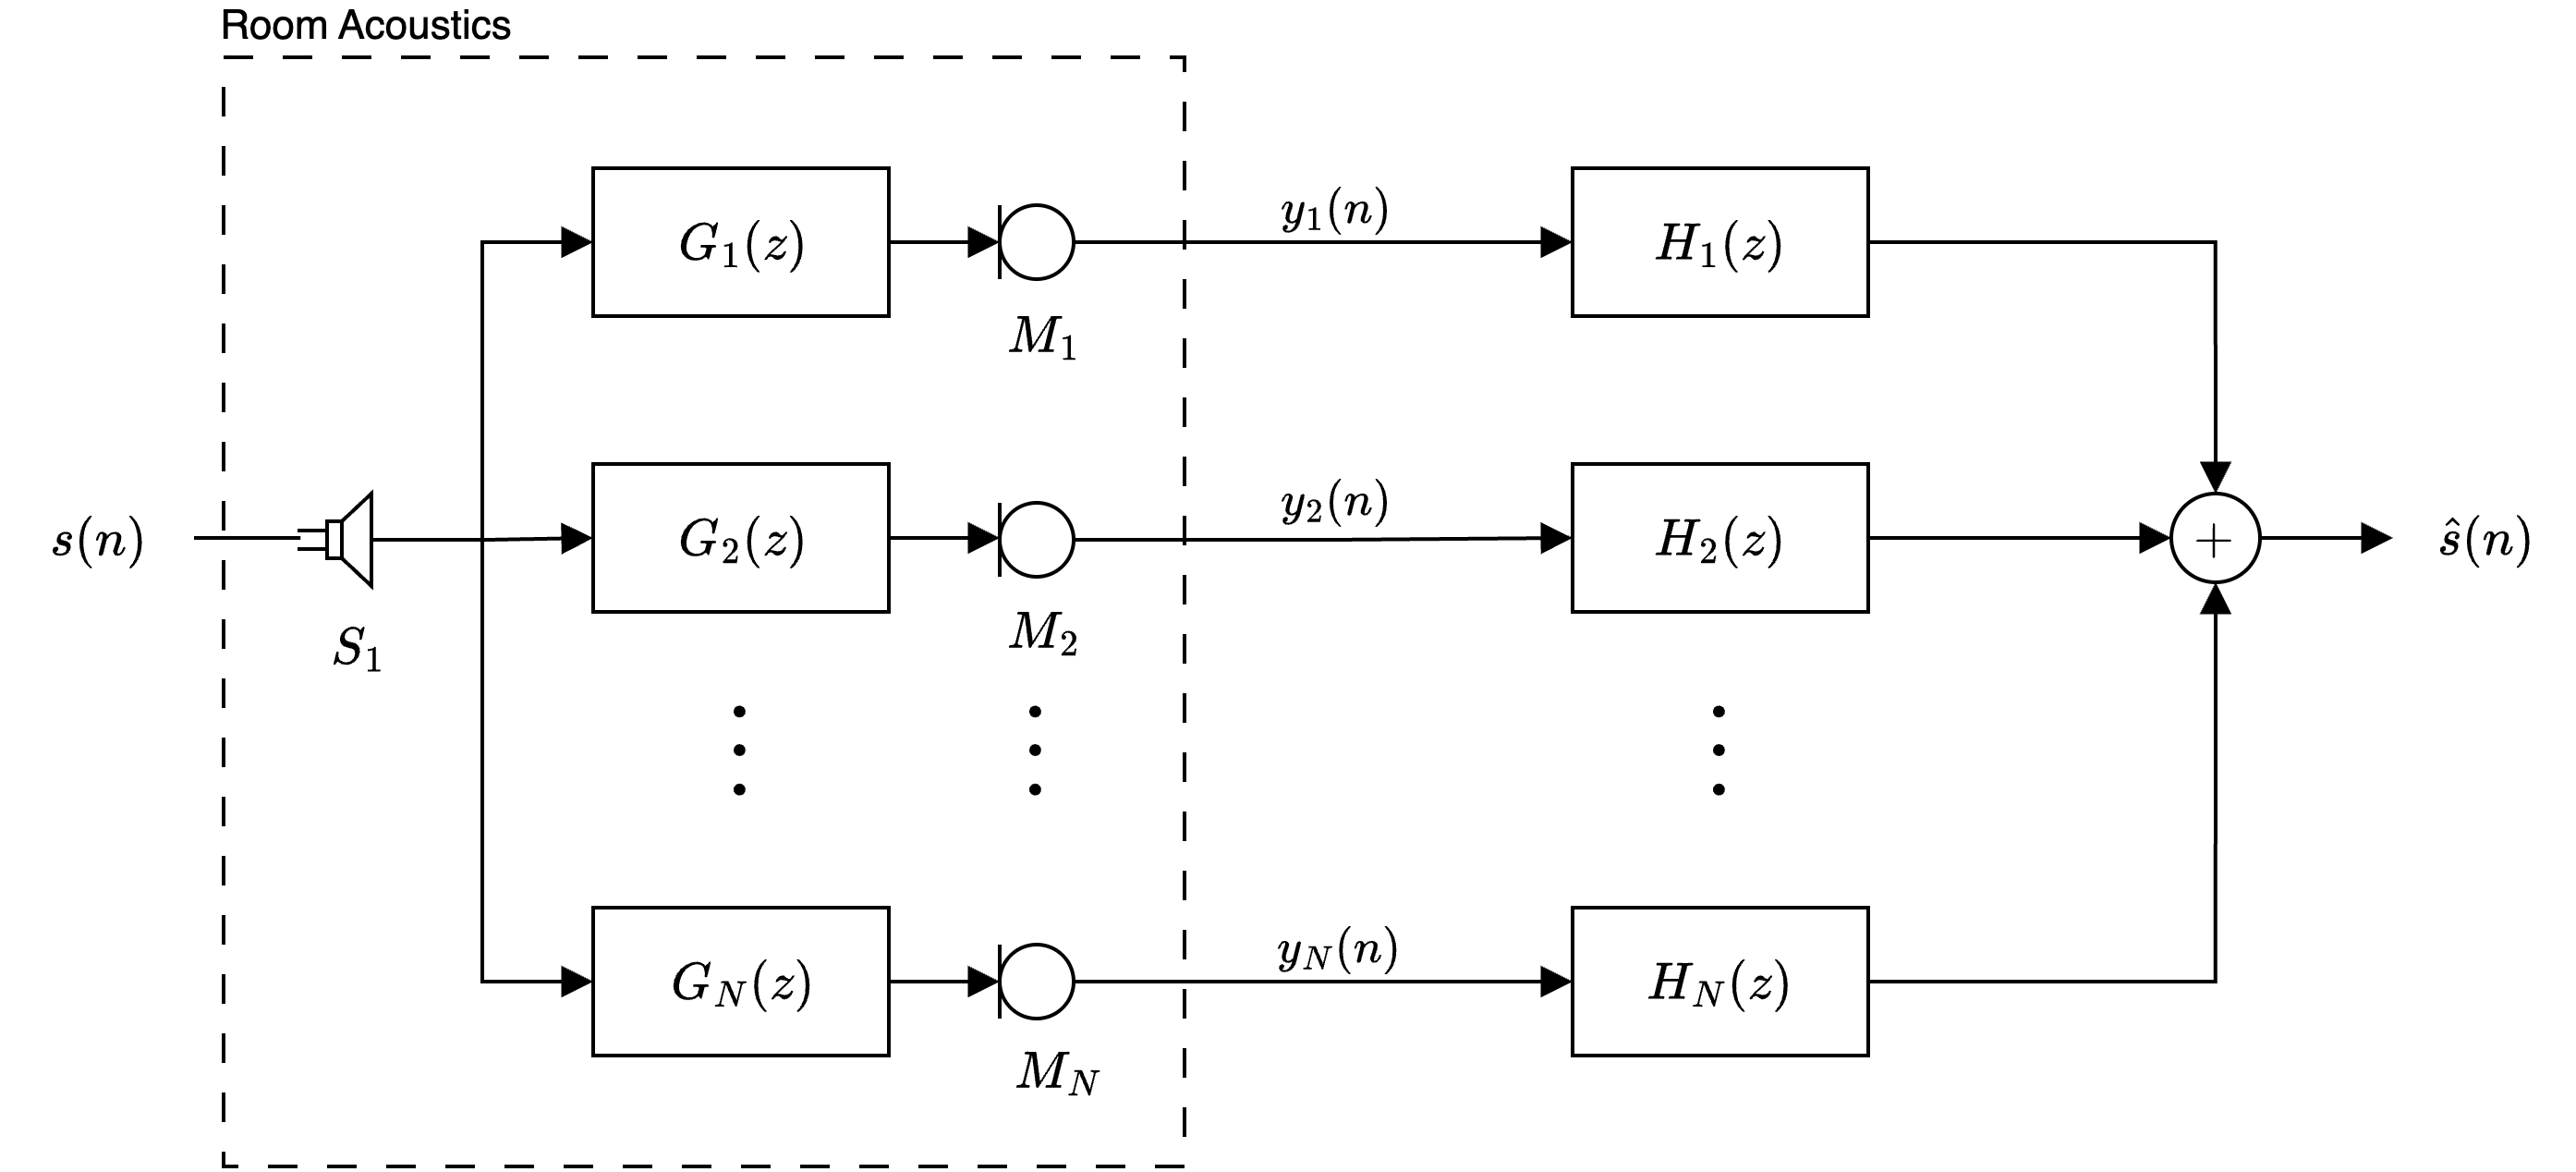
\includegraphics[width=\textwidth]{MINT_SIMO_Dereverb}
		\subcaption{} 
	\end{subfigure}
	\hfill
	\begin{subfigure}[b]{0.49\textwidth}
		\centering
		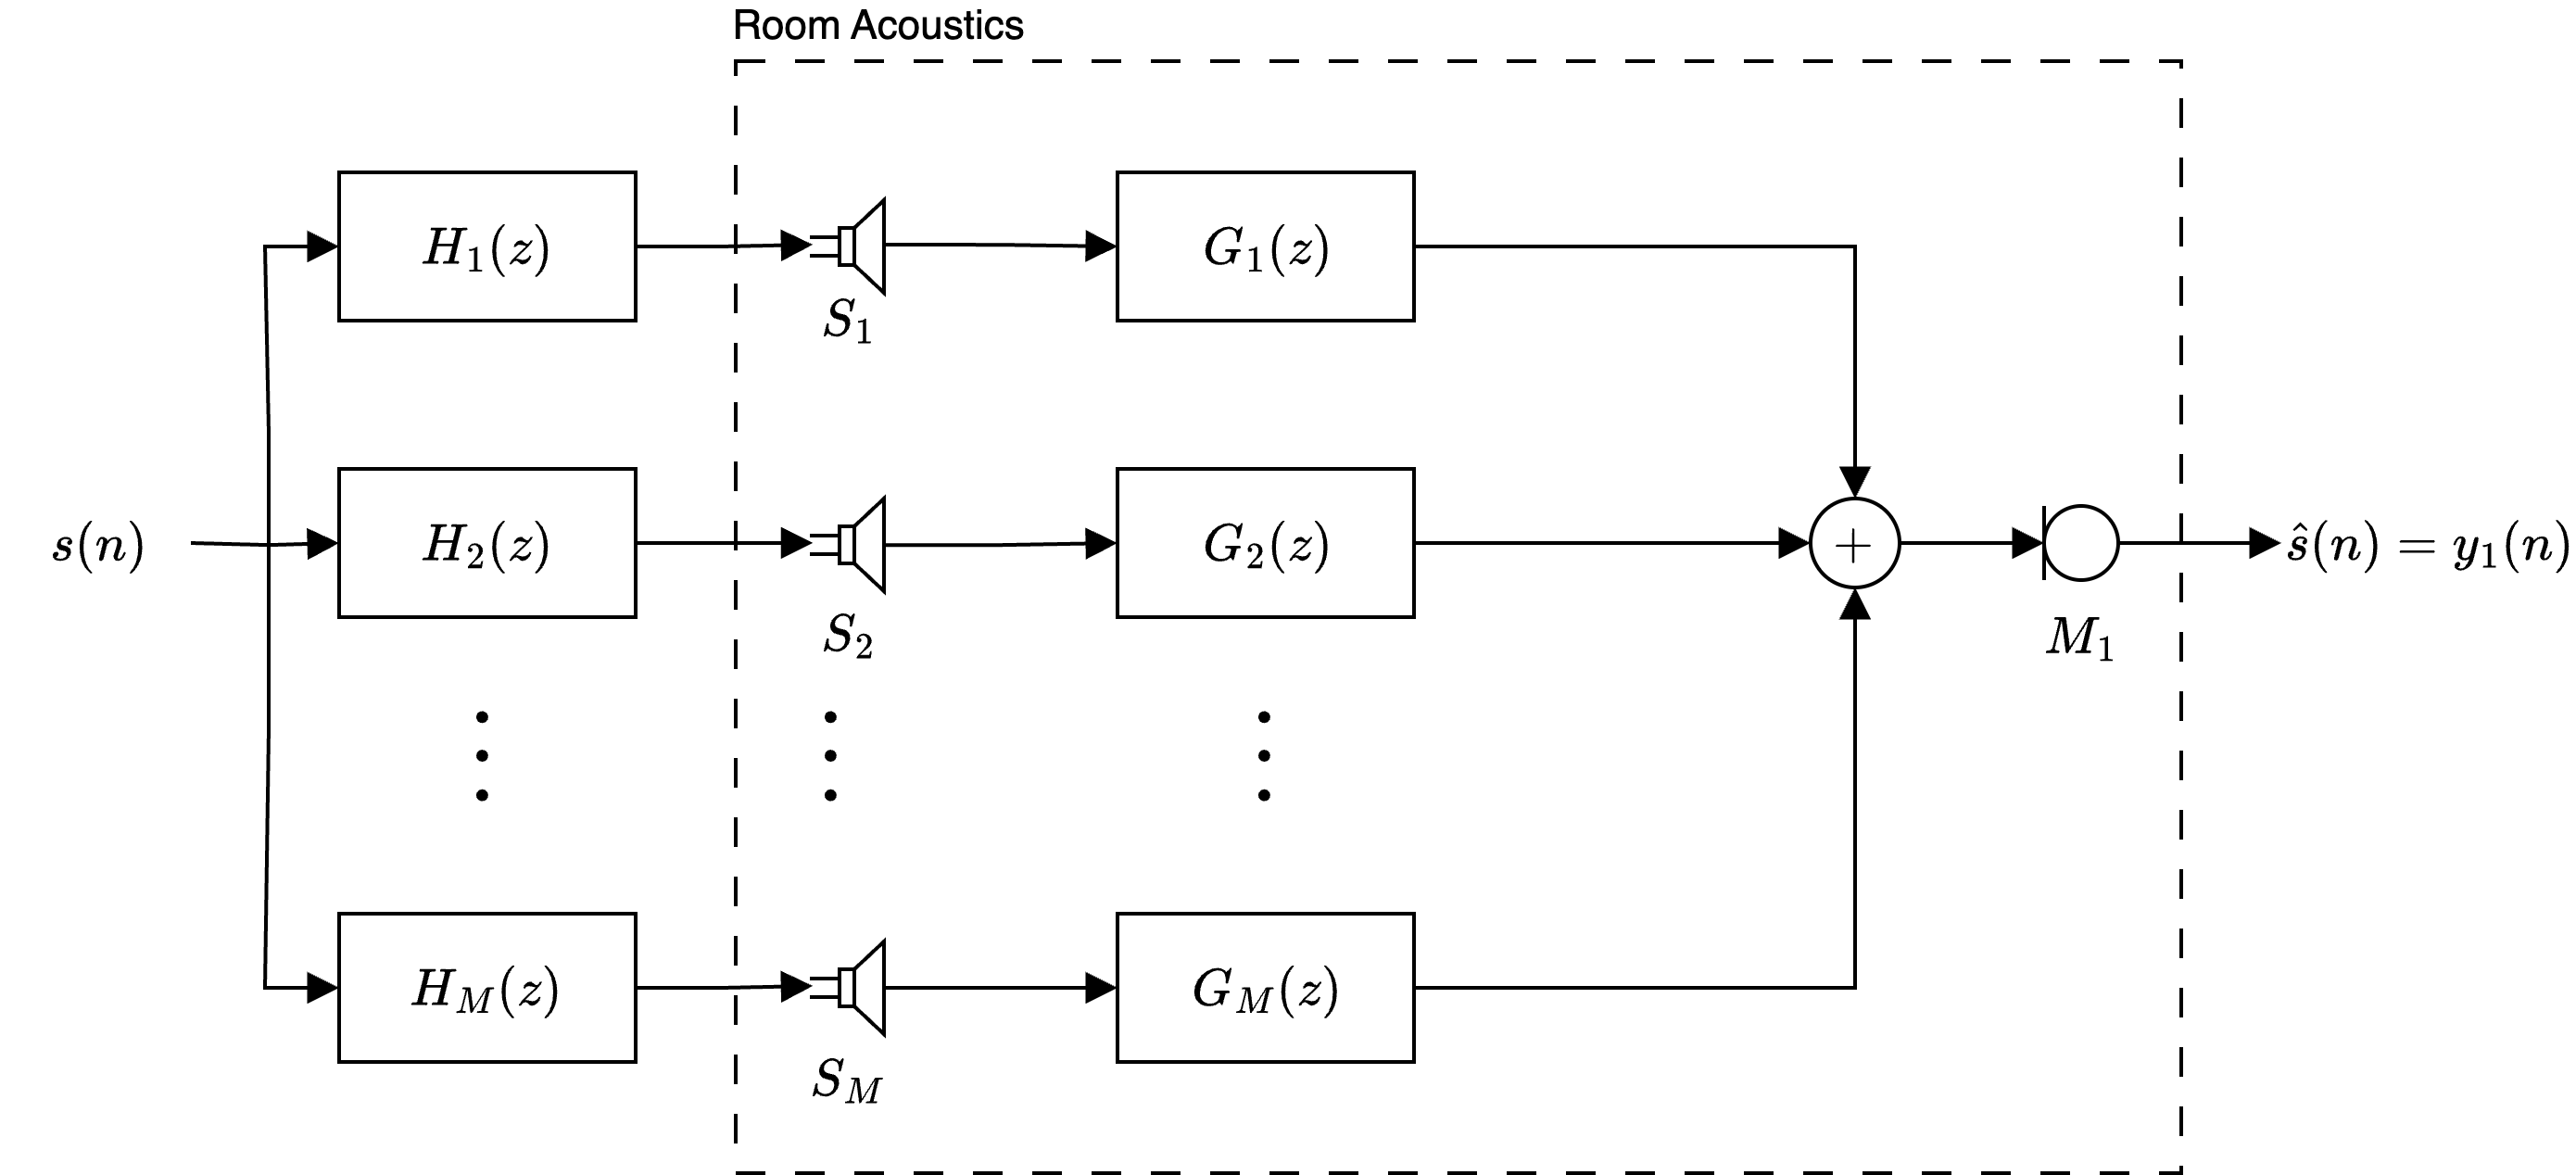
\includegraphics[width=\textwidth]{MINT_MISO_SoundReprod}
		\subcaption{} 
	\end{subfigure}
	\caption[Block diagram for the MISO and SIMO formulations of MINT filtering]{Block diagram the formulations of MINT filtering: dereverberation (a) and sound reproduction (b)}
	\label{fig:MINT_Structures}
\end{figure}

Sound reproduction describes a multiple-input single-output (MISO) system, where each loudspeaker signal is pre-processed with a unique FIR equalizer so as to equalize the RTF at a certain location in the room. Dereverberation describes a single-input multiple-output (SIMO) system where the microphone signals are filtered and summed, with the intention obtaining a clean signal that can be played back elsewhere (e.g., a hearing aid loudspeaker inside the ear canal).

In the SIMO dereverberation case, which is relevant to this thesis, the solution can be derived as follows. Let $g_i(n)$ be the length-$n$ FIR RIR corresponding to acoustic RTF between the source loudspeaker and microphone $i$. Let $h_i(n)$ be the length-$m$ FIR equalizer applied to microphone $i$ before summation with the other channels. 

\begin{eqnarray}
	G_i(z) = Z\{g_i(n)\} = \sum_{k=0}^{n-1}g_i(k)z^{-k} \\
	H_i(z) = Z\{h_i(n)\} = \sum_{k=0}^{m-1}h_i(k)z^{-k} \\
\end{eqnarray}

The inverse filtering problem can be stated in matrix form as

\begin{eqnarray}
	\boldsymbol{G} \boldsymbol{h}=\boldsymbol{d} \label{eq:MINT_problem} \\
	%
	\boldsymbol{G} \boldsymbol{h} =
	\begin{bmatrix}
		\boldsymbol{G}_1 & \boldsymbol{G}_2 & \dots& \boldsymbol{G}_N
	\end{bmatrix} 
	\begin{bmatrix}
		\boldsymbol{h}_1 \\
		\boldsymbol{h}_2 \\
		\vdots \\
		\boldsymbol{h}_N \\
	\end{bmatrix}
	=
	\begin{bmatrix}
		d(0) \\
		d(1) \\
		\vdots \\
		d(m+n-2) \\
	\end{bmatrix} 
	=
	\boldsymbol{d}
\end{eqnarray}

\noindent
where $\boldsymbol{h_i}$ is the vector form of the FIR equalizer applied to microphone $i$, i.e.,

\begin{eqnarray}
	\boldsymbol{h}_i = 
		\begin{bmatrix}
			h_i(0) & h_i(1) & \dots & h_i(m-1)
		\end{bmatrix}^T
\end{eqnarray}

\noindent
and $\boldsymbol{G}_i$ is the Toeplitz convolution matrix which represents the convolution of $g_i(n)$ with $h_i(n)$, i.e.,

\begin{eqnarray}
	\boldsymbol{G}_i = 
	\begin{bmatrix} 
		g_i(0)     & 0           & 0              & \dots    & 0  \\
		g_i(1)     & g_i(0)    & 0              & \dots    & 0  \\
		g_i(2)    & g_i(1)     & g_i(0)      & \dots    & 0  \\
		\vdots    & \vdots    & \vdots     & \ddots & \vdots  \\
		g_i(n-1) & g_i(n-2) & g_i(n-3) & \dots   & 0 \\
		0            & g_i(n-1)  & g_i(n-2) & \dots   & 0 \\
		0            & 0             & g_i(n-1) & \dots   & 0 \\
		\vdots    & \vdots    & \vdots     & \ddots & \vdots  \\
		0            & 0             & 0             & \dots   & g_i(n-1) \\
	\end{bmatrix} 
	\in \mathbb{R}^{(m+n-1)\times m}
\end{eqnarray}

\noindent
To acheive perfect zero-delay equalization, the desired EIR should be $d(n)=\delta(n)$, and therefore

\begin{equation}
	\boldsymbol{d} =
		\begin{bmatrix}
			1 & 0 & \dots & 0
		\end{bmatrix}^T
\end{equation}

Since $\boldsymbol{G} \in \mathbb{R}^{(m+n-1)\times Nm}$, Equation \ref{eq:MINT_problem} represents a problem with $m+n-1$ equations and $Nm$ variables. A perfect solution exists provided $\boldsymbol{G}$ is invertible, which requires that it is square and full rank. For $\boldsymbol{G}$ to be square, that the equalizer filter length, $m$, must be

\begin{equation}
	m = \frac{n-1}{N-1}
\end{equation}

\noindent
Provided $\boldsymbol{G}$ is full rank, the MINT can be computed as

\begin{equation}
	\boldsymbol{h} = \boldsymbol{G}^{-1}\boldsymbol{d}
\end{equation}

For $m < \frac{n-1}{N-1}$, the problem is overdetermined and no perfect solution exists, i.e., it can only be solved by least squares. However, for $m > \frac{n-1}{N-1}$, the problem is underdetermined and therefore has infinite perfect solutions provided its rank is greater than or equal to the number of columns/unknowns. In this case the pseudo-inverse can be used to select the minimum norm solution, i.e.,

\begin{equation}
	\boldsymbol{h} = \boldsymbol{G}^+\boldsymbol{d} = \boldsymbol{G}^T(\boldsymbol{G}\boldsymbol{G}^T)^{-1}\boldsymbol{d}
\end{equation}

%\textbf{Confirm that this form of the psuedo inverse is required for solving an underdetermined system, and is different from the other form which is used for solving an overdetermined system (i.e., least squares)}

 Therefore, for the SIMO dereverberation case, the equalizer filter length, $m$ is required to be

\begin{equation}
	m \ge \frac{n-1}{N-1}
\end{equation}

\noindent
where $m$ is the length of the individual FIR equalizers, $n$ is the length of the individual FIR channels, and $N$ is the number of microphones. Note that although the individual FIR channels are not necessarily the same length, $n$ can be treated as the length of the longest FIR channel.

Equivalently, for the MISO sound reproduction case, the equalizer filter length requirement was shown to be

\begin{equation}
	m \ge \frac{n-1}{M-1}
\end{equation}

\noindent
where $M$ is the number of loudspeakers.


 \cite{miyoshi1986inverse} proved that in order to be invertible (i.e., in order for $\boldsymbol{G}$ to be full rank), there could not be any zeros that were common to all RTFs. It was therefore shown that a MINT equalizer can achieve perfect zero-delay equalization, even when the individual RTFs are non-minimum phase, provided the equalizer filter lengths are sufficiently long and the individual RTFs do not have common zeros anywhere in the z-plane. This result is different from single channel methods which only approach perfect equalization of non-minimum phase channels as the modeling delay approaches infinity. 
 
 It is interesting to note that FIR channels would inheritly have inverse filters that are all-pole and therefore IIR. Single channel FIR equalization of a FIR channel will thus always be approximate, even if the channel is minimum phase. This makes sense intuitively, but \cite{miyoshi1986inverse} also proved this numerically by demonstrating that the matrix formulation of the single channel equalization problem is always overdetermined regardless of equalizer filter length. Remarkably, the MINT can acheive perfect equalization of a FIR channel with individual FIR equalizer filters that are shorter in length than the FIR channels. It is important to remember that real RTFs are not generally speaking FIR, so the MINT is still approximate. However, for a sufficiently long FIR measurement of the true RIR, the residual reflections may be considered negligible.The MINT was proven to greatly outperform the single channel least squares equalization method, acheiving more than \qty{40}{\decibel} additional reverberation attenuation accross all frequencies.
 
In an extended discussion of the MINT,  \cite{miyoshi1988inverse} explored the MIMO case for sound reproduction. They proved that it is possible to perform sound reproduction at $N$ listening positions using $M$ loudspeakers provided the channels had no common zeros,

\begin{equation}
	M > N
\end{equation}

and

\begin{equation}
	m \ge \frac{N(n-1)}{M-N}
\end{equation}

In an extension of the MINT, \cite{nakajima1997sound} proposed the indefinite MINT filter (IMF) which exploits the additional degrees of freedom gained when the FIR equalizer length $m$ is strictly greater than its minimum required length. In this underdetermined case, there are infinite solutions. While the classical MINT recommended using the pseudo inverse to compute the minimum norm solution, IMF makes use of the additional degrees to equalize nearby points. This has the effect of expanding the equalized zone and improving robustness to spatial variation of the RTF.

\subsubsection{Perceptually Motivated Room Response Equalization}

Several authors have proposed extensions to RTF equalization appraoches which constrain the solution to improve perception rather than simply to equalize the channel. This includes the partial MINT \citep[i.e., PMINT][]{kodrasi2012robust}, the relaxed multichannel least-squares \citep{zhang2010use}, and channel shortening \citep{kallinger2006multi}.


\subsection{Blind Deconvolution Problem}

All of the room response equalization approaches discussed in the previous section were dependent on having prior knowledge of the RIR (e.g., by measurement). However, typically in the context of dereverberation, the RIR is not known and must be estimated by other means. The approaches to estimation of a unknown linear system can be divided into supervised methods (i.e., trained/supervised deconvolution) and unsupervised methods (i.e., blind/unsupervised deconvolution).

\subsubsection{The Wiener Filter (Supervised Optimal Filtering)} \label{wiener_filter}

Traditional supervised optimal filtering is formulated as the selection of a filter $H(z)$ which, for a known input sequence $x(n)$, produces a output $y(n)$ that is optimally close (in a mean-squared error sense) to a desired/reference signal $d(n)$. That is, the goal is to design $H(z)$ such that the energy in the error signal $e(n) = d(n)-y(n)$ (as depicted in Figure \ref{fig:WienerFilterProblem}) is minimized. 

\begin{figure}[H]
	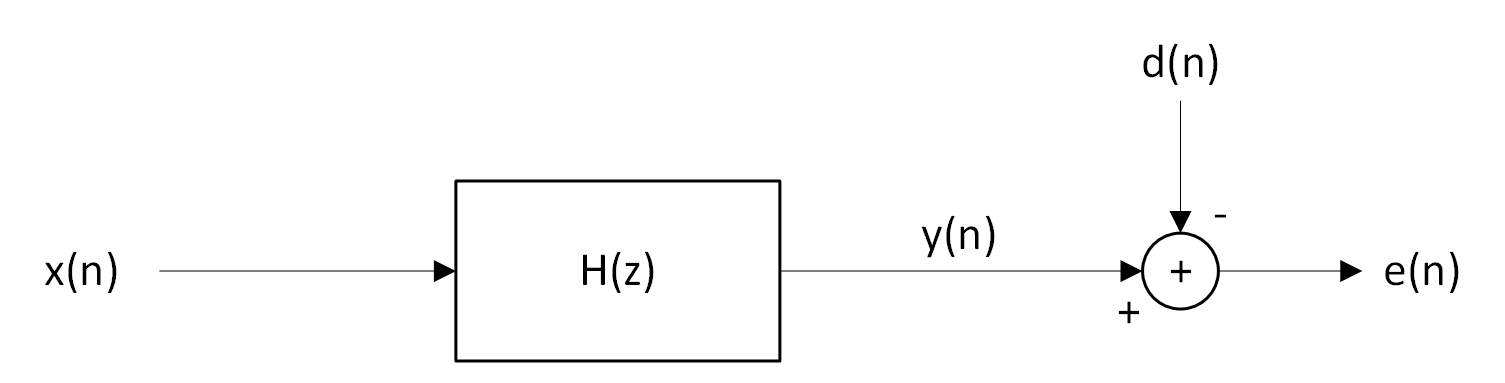
\includegraphics[width = 0.6\textwidth]{WienerFilter}
	\centering
	\caption[Block Diagram for the Wiener filtering problem]{Block diagram for supervised optimal filtering, which attempts to produce a desired output, $d(n)$, from a known input, $x(n)$}
	\label{fig:WienerFilterProblem}
\end{figure}

The derivation for this optimal solution, originally proposed by \cite{wiener1949extrapolation}, is performed in a stochastic framework using expectations for computing mean-squared error. The resulting solution is referred to as the Wiener filter. Considering a length-$N$ FIR filter, $H(z)=\sum_{k=0}^{N-1}h_k z^{-k}$, the cost function $J(\boldsymbol{h})$ is formulated as:

\begin{eqnarray}
	\boldsymbol{x}(n) = 
	\begin{bmatrix}
		x(n) & x(n-1) & \dots & x(n-N+1)
	\end{bmatrix}^T \\
	%
	\boldsymbol{h} = 
	\begin{bmatrix}
		h_0^* & h_1^* & \dots & h_{N-1}^*
	\end{bmatrix}^T \\
	%
	e(n)=d(n) - y(n) = d(n) - \boldsymbol{h}^H\boldsymbol{x}(n) \\
	%
	J(\boldsymbol{h}) = E\left[ \left| e(n) \right|^2 \right] = E\left[e(n)e^H(n)\right] \\
	%
	J(\boldsymbol{h}) = E\left[
	\left(d(n) - \boldsymbol{h}^H\boldsymbol{x}(n)\right)
	\left(d(n) - \boldsymbol{h}^H\boldsymbol{x}(n)\right)^H
	\right] \label{eq:wiener_cost_fn_0} \\
	% 
	J(\boldsymbol{h}) = \sigma_d^2 - \boldsymbol{h}^H\boldsymbol{p} - \boldsymbol{h}^T\boldsymbol{p}^*+\boldsymbol{h}^H R \boldsymbol{h} \label{eq:wiener_quadratic}
\end{eqnarray}

\noindent
where $\boldsymbol{p} = E \left[ \boldsymbol{x}(n)d^*(n) \right]$ is the cross-correlation vector between the input process and the desired/reference process, and $\boldsymbol{R} = E \left[ \boldsymbol{x}(n)\boldsymbol{x}^H (n) \right]$ is the autocorrelation matrix of the input process.

Since the highest-order factor in Equation \ref{eq:wiener_quadratic}, i.e., $\boldsymbol{h}^H \boldsymbol{R} \boldsymbol{h}$ is a quadratic form and the autocorrelation matrix $\boldsymbol{R}$ is Hermitian positive semidefinite (assuming the input process is stationary), $J(\boldsymbol{h})$ represents a quadratic bowl in $N+1$ dimensions with exactly one global minimum. This minimum can be found by taking the derivative of the cost function and setting it equal to zero, i.e.,


\begin{eqnarray}
	%
	\frac{\partial J(\boldsymbol{h})}{\partial \boldsymbol{h}^*}=0 \\
	%
	\boldsymbol{R} \boldsymbol{h} = \boldsymbol{p} \label{eq:wiener_hopf}
\end{eqnarray}

Equation \ref{eq:wiener_hopf} is referred to as the Wiener-Hopf equation and can be solved by any number of methods for solving systems of linear equations. Under the assumption that $x(n)$ is a WSS random process, $\boldsymbol{R}$ is a Toeplitz symmetric matrix, and thus Equation \ref{eq:wiener_hopf} can be solved efficiently via the Levinson-Durbin algorithm. This equation can also be viewed as a stochastic extension of the LS normal equations, and equivalently the Yule-Walker equations in linear prediction. That is, the Wiener filter is optimal for known stationary processes, whereas the LS normal equations produce a filter that is optimal for a known set of data. 

In practice the statistical correlation functions that make up $\boldsymbol{p}$ and $\boldsymbol{R}$ in the Wiener-Hopf equations must be estimated from a finite set of data, and given certain short-term estimation techniques, the Wiener-Hopf equations become identical to the LS normal equations.

The conditioning of the Wiener-Hopf equation is dictated by the eigenvalue spread of the autocorrelation matrix, $\boldsymbol{R}$, which has been shown to be correlated to the dynamic range of the input spectrum (i.e., the “peakiness”). When the input process is white, the eigenvalue spread is equal to 1, and the autocorrelation matrix is the identity matrix. When the input sequence is coloured, the non-zero off-diagonal autocorrelation values result in a larger eigenvalue spread (i.e., higher condition number), which can lead to a less numerically stable solution.

In practice there is always additional sensor noise present which interferes with the measured input, $x(n)$, and/or error signal, $e(n)$. This interference leads to additional misadjustments of the final solution due to distortions in the autocorrelation matrix.

The Wiener filter has also been extended to the optimal derivation of an IIR filter (i.e., the unconstrained Wiener filter), which results in the following frequency domain solution.

\begin{equation}
	\boldsymbol{h}(e^{j\omega}) = \frac{\Phi_{dx}(e^{j\omega})}{\Phi_{xx}(e^{j\omega})}
\end{equation}

\noindent
where $\Phi_{dx}(e^{j\omega})$ is the cross-PSD of $d(n)$ and $x(n)$, and $\Phi_{xx}(e^{j\omega})$ is the PSD of $x(n)$.

The Wiener filter and all resulting adaptive extensions can be applied to both single-channel transversal filters (as described above) and multichannel linear combiners (e.g., beamforming). 

\subsubsection{Supervised Adaptive Filtering} \label{section:adaptive_filter}

To allow tracking of time-varying systems, adaptive algorithms have been proposed which aim to converge on the Wiener filter. Adaptive filtering theory leverages the fact that the MSE cost function forms a quadratic error surface, and generally performs some form of gradient descent to make iterative steps towards the optimal solution. A detailed discussion of the details of adaptive filtering theory can be found in \cite{farhang2013adaptive}, but an overview of the most common algorithms will be provided below.

The steepest descent algorithm (SD) estimates the gradient,

\begin{equation}
	\boldsymbol{\nabla} J(\boldsymbol{h}) = 
	\frac{\partial J(\boldsymbol{h})}{\partial \boldsymbol{h}^*} = \frac{\partial E\left[e(n)e^H(n)\right]}{\partial \boldsymbol{h}^*} \\
\end{equation}


\noindent
of the MSE error surface and steps in the direction opposite to it. The shape of the error surface is dictated by the eigenvalue spread of the autocorrelation matrix for the input sequence, and therefore also the peakiness of the input spectrum. For a white input spectrum, the equal-MSE contours for the error surface are circular, and the negative gradient points directly towards the optimal solution. For more coloured/peaky spectra, the equal-MSE contours of the error surface become elongated, resulting in a negative gradient which does not point directly towards the optimal solution. The Newton descent (ND) algorithm modified SD by deriving the optimal vector-valued step such that the direction of iteration always points directly to the optimal solution regardless of eigenvalue spread

Both SD and ND require estimation of the autocorrelation matrix, $\boldsymbol{R}$, and the cross-correlation vector, $\boldsymbol{p}$. This is computationally expensive, and also it is common for $d(n)$ to be unknown, making $\boldsymbol{p}$ unknown as well. This motivated the usage of the stochastic gradient which is computed solely based on the measured error sequence. The stochastic gradient, defined as

\begin{equation}
	\frac{\partial \left(e(n)e^H(n)\right)}{\partial \boldsymbol{h}^*} = - \boldsymbol{x}(n)e^*(n) \\
\end{equation},

\noindent
represents an instaneous stochastic estimate of the true gradient, $ \frac{\partial E\left[e(n)e^H(n)\right]}{\partial \boldsymbol{h}^*} $.

The commonly used least-mean-squares (LMS) algorithm, steps in the direction of the negative stochastic gradient, using the filter update equation

\begin{equation}
	\boldsymbol{h}(n+1) =
	 \boldsymbol{h}(n) - \mu 	\frac{\partial \left(e(n)e^H(n)\right)}{\partial \boldsymbol{h}^*(n)} =
	 \boldsymbol{h}(n) + \mu \boldsymbol{x}(n)e^*(n)
\end{equation}

\noindent
where $\mu$ is the step size used to control the rate of adaptation. 

The LMS algorithm is very low complexity, does not require prior knowledge/estimation of the statistics of the input process or desired/reference process. The adaptation trajectory of LMS has been shown to match (in the ensemble average) that of the steepest descent algorithm. However, the step size must be carefully selected based an estimate of the eigenvalue spread of the input process to ensure stable convergence.

The Normalized LMS (NLMS) algorithm added a step size that was normalized based on input signal energy so that a standard step size of $\mu=1$ could always be considered optimal (in practice $\mu < 1$ is often required due to numerical error). The NLMS update equation is

\begin{equation}
	\boldsymbol{h}(n+1) =
	\boldsymbol{h}(n) + \mu (n)\boldsymbol{x}(n)e^*(n) = 
	\boldsymbol{h}(n) + \frac{\mu}{\boldsymbol{x}^H(n)\boldsymbol{x}(n) + \varphi} \boldsymbol{x}(n)e^*(n)
\end{equation}

\noindent
where $\varphi$ is a small regularization offset used to avoid filter divergence during periods of very low input energy (i.e., to avoid effective division by zero).

Separate from gradient-based algorithms described above, the recursive least squares (RLS) algorithm forms an adaptive extension of least squares optimization. This data-centric approach minimizes deterministic total-squared-error for the specific data observed. RLS performs LS optimization over all data observed since the start of time, with an added forgetting factor to allow tracking of time-varying systems.

As was the case with Wiener filtering, in practice there is additional sensor noise present in the measured input signal, $x(n)$, and/or error signal, $e(n)$, which interferes with the adaptation and leads to misadjustments. This can be particularly problematic when the interfering noise is correlated with itself.

All adaptive algorithms are derived in the complex domain to allow implementation in the frequency domain and subband domain. Adaptation in the frequency/subband domain is often desirable for computational efficiency and to allow control of the adaptation on a frequency-selective basis. Additionally, convergence tends to be faster in the frequency/subband since narrowband signals tend to have flatter spectra than wideband signals. However, the DFT/Inverse DFT or subband filterbank adds computational complexity and memory of its own, and increases system latency which may not be desirable.


\subsubsection{Blind Deconvolution Challenges}

When applied to system equalization (e.g., RTF equalization), as depicted in Figure \ref{fig:supervised_inverse_filter}, the desired/reference signal is the input to the unknown system, i.e., $d(n)=s(n)$, and input to the equalizer filter, $H(z)$, is the output of the unknown system, i.e., $x(n)=s(n)*h(n)$. 

\begin{figure}[H]
	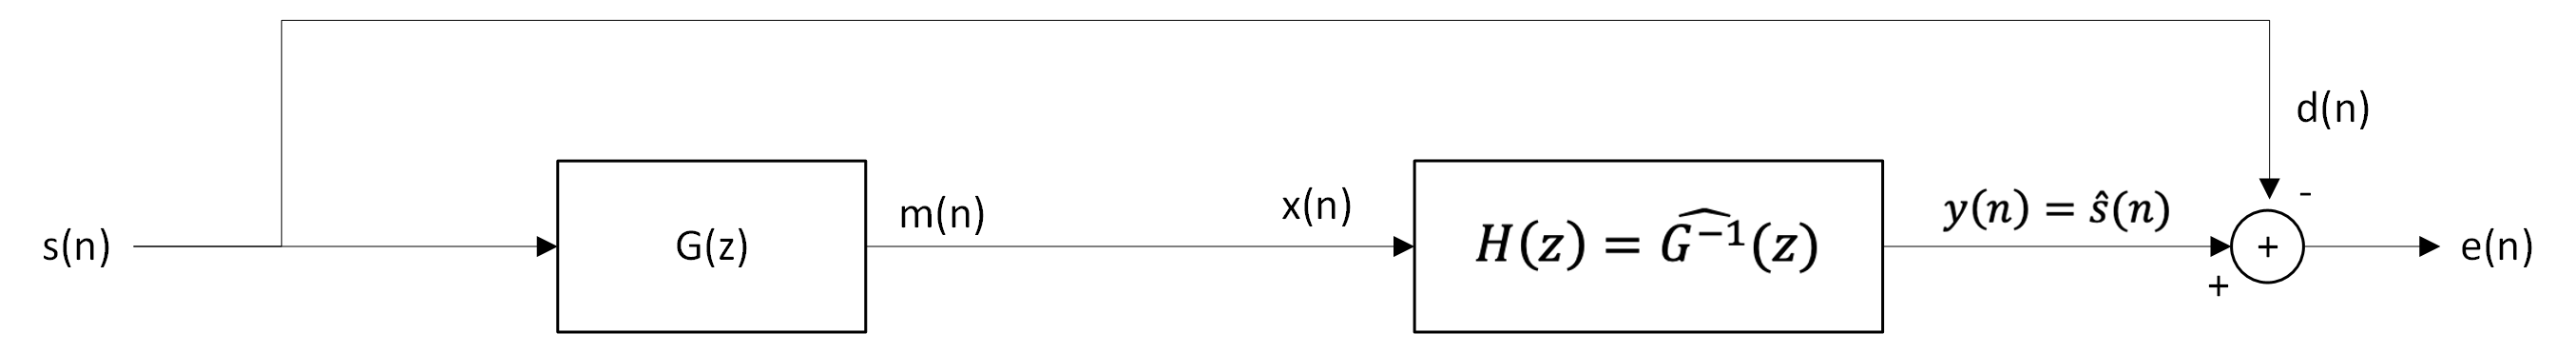
\includegraphics[width = \textwidth]{supervised_inverse_filter}
	\centering
	\caption[Block diagram for the supervised inverse filtering problem]{Block diagram for supervised inverse filtering / equalization, which attempts to produce reproduce the known input, $s(n)$, to an unknown system $G(z)$, from the measured system output, $y(n)$, using a filter, $H(z)$}
	\label{fig:supervised_inverse_filter}
\end{figure}

Blind deconvolution (i.e., unsupervised inverse filtering) refers to the problem of inverse filtering when the input, $s(n)$, to the unknown system, $G(z)$, is unknown as well. This generally requires two stages: unsupervized estimation of the unknown  (i.e., blind system identification, or BSI), and inverse filtering. This implies that the error signal $e(n)$ is unknown. For completeness, measurement noise, $v(n)$, is included (Figure \ref{fig:blind_deconvolution}).

\begin{figure}[H]
	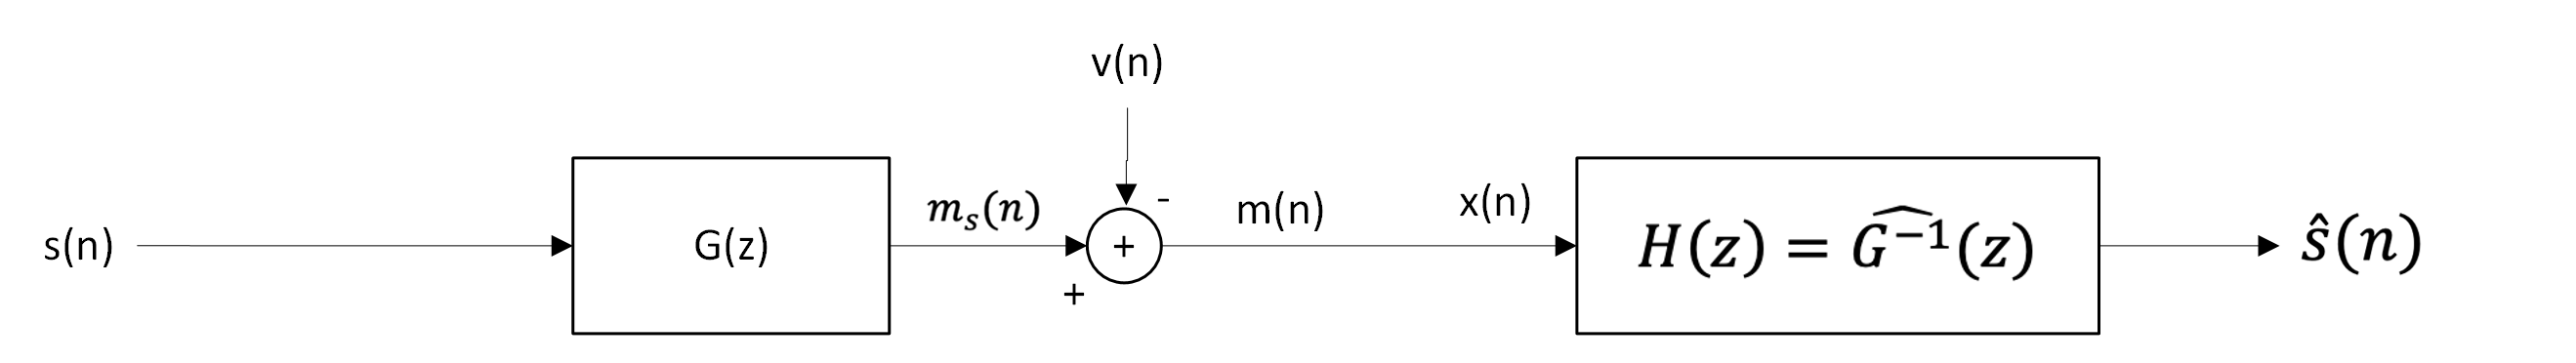
\includegraphics[width = \textwidth]{blind_deconvolution}
	\centering
	\caption[Block diagram for the blind deconvolution problem]{Block diagram for blind deconvolution, which attempts to produce reproduce the unknown input, $s(n)$, to an unknown system $G(z)$, from the measured system output, $y(n)$, including additive noise $v(n)$, using a filter, $H(z)$}
	\label{fig:blind_deconvolution}
\end{figure}

Speech dereverberation is generally a blind problem since the source is a human talker, and the corresponding speech signal is only measured at the listening point (i.e., only the RTF system output is available). This creates a challenging problem since the system input, $s(n)$, and system itself, $G(z)$, are both unknown and must be derived from the measured signal at the output, $y(n)$ (i.e., microphone signal). Therefore, there is an ambiguity as to whether the poles and zeros of the measured output signal correspond to the input signal or the system.

In the context of blind wireless channel equalization, the unknown source often falls into a discrete set of known symbols that are stationary within a symbol period. This can be exploited to make assumptions about the source when estimating the system. Conversely, in speech dereverberation the speech signal is virtually arbitrary and highly non-stationary, making the problem even more challenging.

Additionally, as discussed in Section \ref{RIR_Invertibility}, reverberant channels vary significantly with respect to spatial location and slight misadjustments to the equalizer can result in making the effects of reverberation worse. This spatial variance results in a highly time-varying channel, which must be tracked adaptively. Also, as discussed, RTFs tend to be non-minimum-phase thus not having a causal stable single-channel inverse, and may have strong or perfect zeros which can result in severe narrowband noise amplification.

As with traditional supervised system equalization, interfering noise can result in misconvergence of the inverse filter, and must be handled accordingly.

Lastly, since reverberation times can be in the order of several seconds, resulting in sampled RIRs spanning thousands or even tens of thousands of taps, computations in reverberation cancellation also tend to be very complex and sensitive to numerical error.

\subsubsection{Practical Blind Deconvolution in Wireless Systems}

The topic of blind deconvolution originated in geophysics and wireless communication, and has been studied extensively in these fields. A full discussion of the topic of blind wireless channel inversion can be found in \cite{ding2018blind}, but some of the most common practical approaches will be summarized here. As will be shown, these approaches generally rely on assumptions about the source signal which do not hold in the context of speech dereverberation.

In wireless systems, where the input signal is controlled by a radio base station and the output is detected by a mobile phone, often a periodic training sequence (i.e., a reference symbol) is used as a reference for performing periodic supervised adaptive channel estimation. However to provide continuous tracking of the time-varying channel without using too much channel bandwidth for reference symbols, additional unsupervised adaption is often employed.

The first unsupervised approach, proposed by \cite{lucky1965automatic}, was the so-called decision-directed approach, in which the system which toggled between supervised and unsupervised adaptation periodically. A non-linear decision device at the output of the equalizer was used to select the most likely symbol (e.g., closest symbol in the magnitude-phase symbol constellation), and during periods of unsupervised adaptation this estimated symbol was used as the desired equalizer output to make adaptations. This concept was highly reliant on the theory of Bussgang statistics which allows important assumptions about the statistics of a stochastic process before and after a memoryless non-linear operation. This approach has been shown to work well provided the channel is slowly time-varying and there is minimal misconvergence during supervised training so that deviations during unsupervised training are minimal. Building on this concept the Sato method \citep{sato1975method} and the Constant Modulus algorithm \citep{godard1980self} were proposed which improved robustness to larger deviations by adapting using an error metric between measured signal and the set of possible symbols, instead of a hard symbol decision. 

These algorithms laid the groundwork for the approaches used in practice, most of which rely on the fact that the transmitted symbols may only fall into a set of known symbols. This assumption of course does not hold for speech dereverberation where the source signal is highly non-stationary speech. Truly blind adaptation without exploiting knowledge of a symbol dictionary, which has applications in speech dereverberation, will be explored in the subsequent sections.

\subsubsection{SOS and HOS Methods for Blind System Identification}

Techniques for BSI can generally by categorized by their usage of second order statistics (SOS) or higher order statistics (HOS). 

It is well understood that SOS such as autocorrelation and power spectrum only capture the magnitude information of a signal, and do not directly capture any phase information. Referring back to Figure \ref{fig:blind_deconvolution}, the power spectrum of the system output, $y(n)$, (neglecting noise) is given by

\begin{equation}
	S_{yy}(\omega) = |G(\omega)|^2 S_{ss}(\omega)
\end{equation}

\noindent
Therefore, if only the SOS of the system output is known, then only the magnitude response of the channel, $|G(\omega)|$, can be identified. For this reason, SOS methods for BSI are limited in their ability to perfectly identify the true underlying system. Since the phase response of an RTF contains significant reverberant energy (Section \ref{homomorphic_eq}), this has a strong impact on dereverberation performance. Also note that correct identification of $|G(\omega)|$ from only the SOS of the system's output, $S_{yy}(\omega)$, additionally requires knowledge of the SOS of the system's input, $S_{ss}(\omega)$. As such, truly blind estimation of $|G(\omega)|$ requires that the input is white and stationary (i.e., independent and identically distributed, i.i.d., up to the 2nd order).

In the seminal work by \cite{giannakis1989identification}, it was shown that the complete magnitude and phase information of an LTI system are captured in the HOS of the system's output. Specifically, it was shown that the magnitude and phase information are retreivable from the $k$-order cumulant or the $(k-1)$-order polyspectrum of the system's output for $k>2$, provided the input is non-Gaussian (i.e., it has non-zero HOS). Similar to the SOS case, identification of the system, $G(z)$, from only the HOS of the system's output requires knowledge of the HOS of the input, or equivalently assumes that the input is i.i.d. up to the $k$\textsuperscript{th} order. If the input is not i.i.d., the identified system will include the source statistics, and therefore the designed equalizer will whiten the source as well. To avoid this undesired result, additional processing is needed to estimate and restore the source spectrum.

In practice, HOS methods are not often used for dereverberation due to the massive amount of signal data needed to reduce the high level of variance that arises in numerical estimates of HOS. This data constraint results in high computational complexity and greatly reduces the ability of algorithms to track time-varying channels.
	
\subsubsection{Multichannel SOS Methods for Blind System Identification} \label{mc_sos_bsi}

In the previous section, it was explained that SOS do not capture phase information, which can severely impact dereverberation performance. However, it has been shown that using multiple channels, partial phase information can be captured. Originally demonstrated by \cite{slock1994blind}, the spatial diversity gained from a multichannel setup gives rise to spatial cross-correlations from which relative phase information can be extracted. In the context of dereverberation, this is realized using multiple microphones. Since only the relative phase is known, the system can only be identified up to a linear-phase term.

Additionally, the spatial diversity gained by using multiple microphones provides a mechanism for mitigating the source/filter ambiguity that is inherit to the BSI problem. Intuitively, if the poles and zeros of each microphone signals are known (or can be estimated), the source components will be common to all microphone signals, while the channel/filter components will be different for each microphone. Therefore, it is possible to uniquely identify the channel RTFs provided there are no poles or zeros that are common to all channels.

As discussed in Section \ref{MINT}, the usage of multiple channels in equalizer design also makes it possible to perfectly equalize non-minimum phase systems (i.e., a MINT equalizer). This is possible provided the MINT conditions are met, i.e., the individual channel RTFs do not share common zeros and the individual FIR equalizer filters are of length $m \ge \frac{n-1}{N-1}$, where $n$ is the length of the individual RIRs and N is the number of microphones. Multichannel SOS methods for BSI can thus be viewed as a blind estimation of the MINT equalizer.

In summary, using multiple microphones, it is possible to identify an arbitrary multichannel RTF from only its output signals for any arbitrary source signal, provided the individual channels do not share common poles/zeros. Using a multichannel inverse filter, it is also possible to perfectly equalize this channel up to a gain factor and linear-phase term provided the MINT conditions are met. These properties, and the relatively small amount of data required to compute SOS, have given rise to a number of blind deconvolution methods for derverberation, which will be discussed in the following section.

\subsection{Multichannel SOS Methods for Reverberation Cancellation}

This section outlines existing methods for dereverberation by blind deconvolution using multichannel SOS methods for BSI. While all the following methods rely on multichannel SOS to separate the poles and zeros of the RTF from those of the source signal, they differ in the details of how this is done.

The Multichannel equalization problem is shown in Figure \ref{fig:MC_EQ}

\begin{figure}[H]
	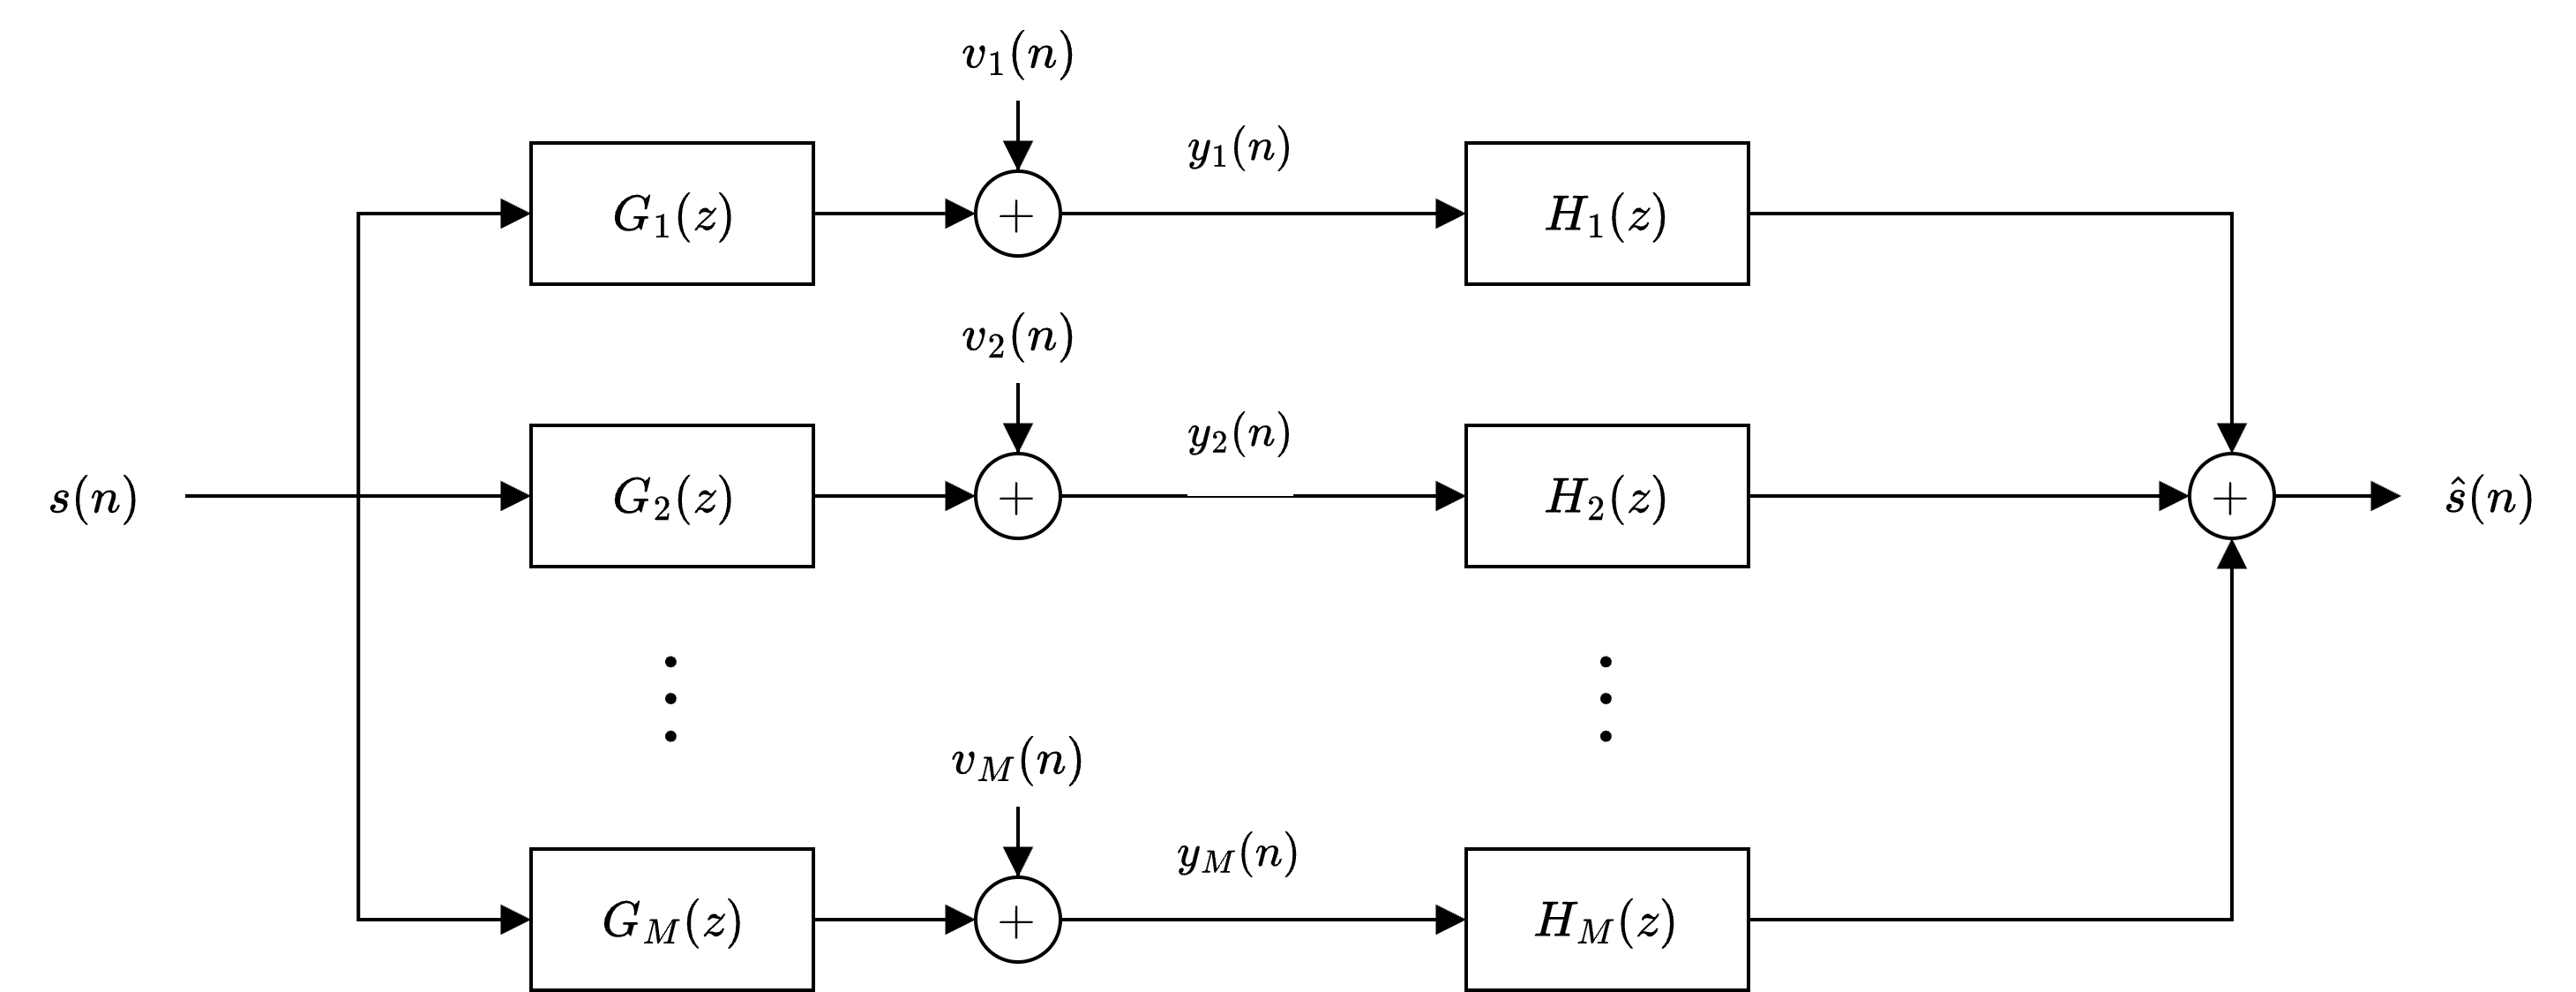
\includegraphics[width = \textwidth]{MC_EQ}
	\centering
	\caption[Block diagram for the multichannel inverse filtering problem]{Block diagram for multichannel inverse filtering, which attempts to produce reproduce the known input, $s(n)$, to an unknown multichannel system $\{G_1(z), G_2(z), \dots, G_M(z)\}$, by filtering and summing the $M$ microphone signals, $\{y_1(n), y_2(n), \dots, y_M(n)\}$, with a set of FIR filters, $\{H_1(z), H_2(z), \dots, H_M(z)\}$}.
	\label{fig:MC_EQ}
\end{figure}

$G_k(z)$ will be used to denote the RTF from the source to the $k$th microphone, and $H_k(z)$ will be used to denote the FIR equalizer filter applied to microphone signal $k$ before summation with the other channels. $M$ will be used to denote the number of microphones/channels.


\subsubsection{Homomorphic Deconvolution}

One of the earliest proposed methods to blind deconvolution was accomplished in the complex cepstral domain \citep{oppenheim1976digital}. The complex cepstrum of a clean speech signal has been shown to be concentrated around the zero quefrencies, while complex cepstrum of the RIR tend to be concentrated at higher quefrencies. As such a simple single-channel blind deconvolution technique consists of applying a window function (i.e., a short-pass lifter) to the complex cepstrum which attenuates the higher quefrencies. However, this effectively results in a minimum phase modeling of the system, which severely limits dereverberation performance. \cite{petropulu1994cepstrum} proposed a multichannel extension of this approach, and showed that an arbitrary mixed-phase RIR could be estimated from just the phases of two microphone signals. However, all homomorphic deconvolution methods tend to lead to severe speech distortions, and their performance is severely limited by the selection of the window function cutoff. 


\subsubsection{Subspace Methods}

Several methods have been proposed which build on a key observation from \cite{gurelli1995evam} that the RIRs of multiple channels can be extracted from the null space of the multichannel microphone data matrix. This was originally demonstrated in a two-channel noise-free configuration, where a source signal $s(n)$ is passed through two channels with RIRs $g_1(n)$ and $g_2(n)$, producing microphone signals,$y_1(n)$ and $y_2(n)$.

\noindent
\begin{eqnarray}
	y_1(n) = s(n)*g_1(n) \\
	y_2(n) = s(n)*g_2(n)
\end{eqnarray}

Conceptually, if each RIR is applied as a filter to the opposite microphone signal, the difference between the resulting signals should be zero, i.e., the so-called cross relation equality,

\noindent
\begin{equation}
	y_1(n)*g_2(n) - y_2(n)*g_1(n) = s(n)*g_1(n)*g_2(n) - s(n)*g_2(n)*g_1(n) = 0 \label{eq:cross_relation}
\end{equation}

\cite{gurelli1995evam} proved that the RIRs were consequently identical to the null space eigen-vectors of the multichannel data matrix (i.e., the data matrix of $y_1(n)$ and $y_2(n)$). A similar proof was shown to hold for an arbitrary number of channels. 

In the presence of noise, the multichannel data matrix generally does not have a null space since Equation \ref{eq:cross_relation} will not produce a difference of zero. Instead, the RIRs are extracted from the so-called ``noise subspace" which is defined to have the smallest eigenvalues (i.e., minimizes cross-relation error).

Several more practical algorithms have been proposed to more heuristically minimize the cross-relation error, often using an adpative algorithm such as LMS, NLMS or RLS \citep[][]{identification1995least, huang2003class, huang2002adaptive}.

In addition to the requirements already stated for BSI to be possible with multichannel SOS, this method also requires that the channel orders are known exactly so that the multichannel data matrix can be sized correctly. If the channel orders are over-estimated, the produced RIR estimates will include a common term of arbitrary extra zeros, $e(n)$, since

\begin{equation}
	s(n)*g_1(n)*g_2(n)*e(n) - s(n)*g_2(n)*g_1(n)*e(n) = 0
\end{equation}

\noindent
which will degrade performance. This is a severe limitation of technique, and for this reason subspace methods are not often useful in practice.


\subsubsection{Multichannel Linear Prediction Methods}  \label{section_dap}

While multichannel linear prediction is a well understood topic with many high-level descriptions such as the one provided in \cite{naylor2010speech}, no detailed derivation or final solution for the multichannel Yule-Walker equations was found during literature review. Therefore the solution was derived and presented in detail below.

%\paragraph{Multichannel Linear Prediction Theory} 
\noindent
\textbf{Multichannel Linear Prediction Theory}

As discussed in Section \ref{linear_prediction}, linear prediction models speech as an autoregressive process, and consequently the prediction error filter $\left(A(z)=1-\sum_{k=1}^{p}a_k z^{-k}\right)$ removes autocorrelation from the signals and thus acts as a whitening filter. Conceptually we can model a speech signal, $s(n)$, as the excitation of an all-pole filter with an uncorrelated input sequence, 

\begin{equation}
	S(z)=Z\{s(n)\}=U(z) \frac{1}{1 - \sum_{k=1}^{p}a_k z^{-k}}  = U(z) S_{\mathrm{AP}}(z)
\end{equation}

\noindent
where $S_{AP}(z)$ is an all-pole filter encapsulating all autocorrelation in $s(n)$, and $U(z)$ is the Z-transform of the uncorrelated residual part of $s(n)$  that does not fit the autoregressive model. The linear prediction ``inverse filter" $\left(\frac{1}{A(z)} =\frac{1}{1 - \sum_{k=1}^{p}\alpha_k z^{-k}}\right)$  is an estimate of that all-pole model, i.e., of $S_{\mathrm{AP}}(z) = \frac{1}{1 - \sum_{k=1}^{p}a_k z^{-k}}$. 

If we extend this modeling concept to a reverberant speech signal, $y(n)$, that is produced by filtering $s(n)$ with an RIR, $g(n)$, we get

\begin{equation}
	Y(z) = S(z) G(z) = \tilde{U}(z) S_{\mathrm{AP}}(z) G_{\mathrm{AP}}(z)
\end{equation}


\noindent
where $G_{\mathrm{AP}}(z)$ is an all-pole model of $G(z)$, and $\tilde{U}(z)$ encapsulates the uncorrelated residual part of both $s(n)$  and $g(n)$ that does not fit the autoregressive model. As described in Section \ref{dt_speech_model}, an arbitrary transfer function can be perfectly represented by an infinite number of poles and can be represented reasonably with a sufficient number of poles.

Since linear prediction estimates $S_{\mathrm{AP}}(z)G_{\mathrm{AP}}(z)$ without any knowledge of the input sequence $s(n)$, it effectively performs blind system identification, and the prediction error filter fascilitates blind deconvolution. However, the prediction error filter will also remove the autoregressive properties of the source signal, which will result in over-whitening of the speech signal. The handling of this will be discussed later.

As proved by the MINT (Section \ref{MINT}), it is theoretically possible to perfectly identify and equalize an arbitrary RTF by using multiple channels. For this reason, multichannel linear prediction has proven to be one of the most promising approaches to blind deconvolution for dereverberation. The multichannel extension of linear prediction in the context of equalizing a multichannel system is formulated as shown in Figure \ref{fig:MC_LPC}

\begin{figure}[H]
	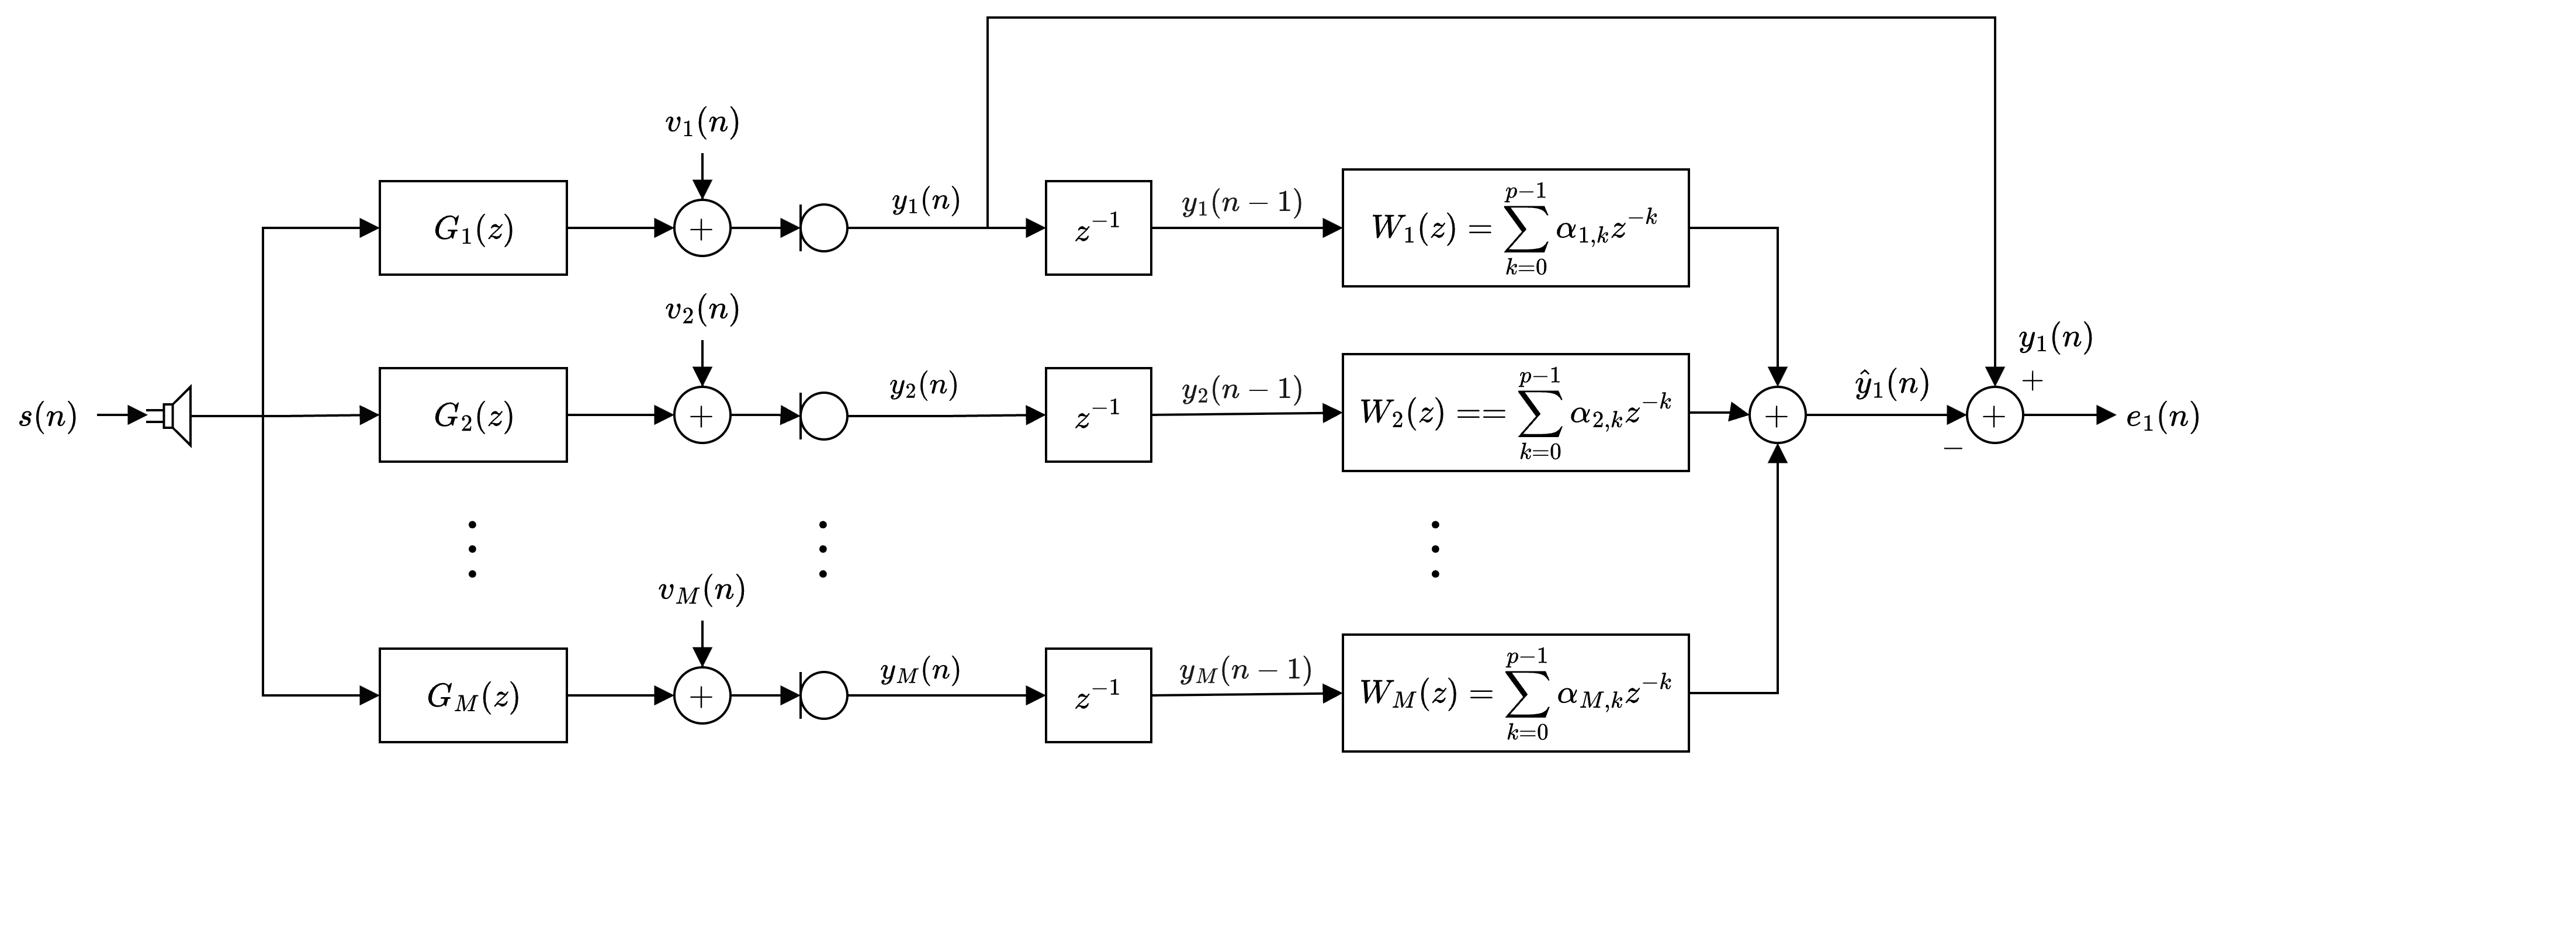
\includegraphics[width = \textwidth]{MC_LPC}
	\centering
	\caption[Block diagram for the multichannel linear-predictive inverse filtering]{Block diagram for multichannel linear prediction applied to channel equalization, where an estimate of reverberant microphone signal 1 is produced by filtering and summing past samples of reverberant microphone signals 1-$M$}.
	\label{fig:MC_LPC}
\end{figure}

As shown, the current samples of $y_1(n)$ are estimated by filtering and summing the past $p$ samples of all $M$ microphone signals. Note that since all output signals reflect the same source data, $s(n)$, it is important that the output signals are time-aligned. This is necessary so that the window of source data included in the delayed signals, $\{y_1(n-1), \dots, y_M(n-1)\}$), indeed lags the data included in $y_1(n)$ by 1 sample. If the signals are not aligned in this way, the prediction error filter will cancel $y_1(n)$ instead of whitening it.

The prediction error signal $e_1(n)$ is thus

\noindent
\begin{equation}
	e_1(n) = y_1(n) - \hat{y}_1(n)) = y_1(n) -\sum_{m=1}^{M} \sum_{k=1}^{p} \alpha_{m,k} y_m(n-k) \label{eq:mc_lp_error}
\end{equation}

\noindent
which can be represented in vector form as

\begin{eqnarray}
	e_1(n)=y_1(n) - \sum_{k=1}^{p} \boldsymbol{\alpha}_k^T \boldsymbol{y}(n-k) \\
	e_1(n) = y_1(n) - \boldsymbol{\tilde{\alpha}}^T \boldsymbol{\tilde{y}}(n-1) \label{eq:mc_lp_error_vec}
\end{eqnarray}

\noindent
with
\begin{eqnarray}
	\boldsymbol{y}(n) = 
	\begin{bmatrix}
		y_1(n) &	y_2(n)  & \dots  & y_M(n)  \\
	\end{bmatrix}^T  \in  \mathbb{R} ^ {M \times 1} \\
	%
	\boldsymbol{\alpha}_k = 
	\begin{bmatrix}
		\alpha_{1,k} &	\alpha_{2,k} & \dots  & \alpha_{M,k} \\
	\end{bmatrix}^T  \in  \mathbb{R} ^ {M \times 1}
\end{eqnarray}

\noindent
and
\begin{eqnarray}
	\boldsymbol{\tilde{y}}(n-1) = 
	\begin{bmatrix}
		\boldsymbol{y}^T(n-1) &	\boldsymbol{y}^T(n-2)  & \dots  & \boldsymbol{y}^T(n-p)   \\
	\end{bmatrix}^T  \in  \mathbb{R} ^ {Mp \times 1}\\
	%
	\boldsymbol{\tilde{\alpha}} = 
	\begin{bmatrix}
		\boldsymbol{\alpha}^T_1 &	\boldsymbol{\alpha}^T_2  & \dots  & \boldsymbol{\alpha}^T_p \\
	\end{bmatrix}^T  \in  \mathbb{R} ^ {Mp \times 1}
\end{eqnarray}


It is more common, however, to formulate multichannel linear prediction as estimating the sample of a vector-valued signal, $\boldsymbol{y}(n)$, from its past $p$ vector-valued samples. This results in a vector-valued error signal, $\boldsymbol{e}(n) = \begin{bmatrix} e_1(n) & e_2(n) & \dots& e_M(n) \end{bmatrix}^T$, defined as

\begin{eqnarray}
	\boldsymbol{e}(n) = \boldsymbol{y}(n) - \boldsymbol{\hat{y}}(n) = \boldsymbol{y}(n) - \sum_{k=1}^{p} \boldsymbol{A}_k \boldsymbol{y}(n-k)  \label{eq:mc_lp_error_parallel}
\end{eqnarray}

\noindent
where $\boldsymbol{A}_k \in  \mathbb{R} ^ {M\times M}$ is the multichannel prediction coefficient matrix for a $k$-sample delay. This can also be fully encapsulated in vector form as

\begin{equation}
	\boldsymbol{e}(n)= \boldsymbol{y}(n) - \boldsymbol{A}_{\mathrm{mc}} \tilde{\boldsymbol{y}}(n-1) \label{eq:mc_lp_error_vec_parallel}
\end{equation}

\noindent
where

\begin{eqnarray}
	\boldsymbol{A}_{\mathrm{mc}} = \begin{bmatrix}
		\boldsymbol{A}_1 & \boldsymbol{A}_2 & \dots& \boldsymbol{A}_p
	\end{bmatrix} \in \mathbb{R}^{M \times Mp}
\end{eqnarray}

\noindent
Note that the first row of Equation \ref{eq:mc_lp_error_vec_parallel} is exactly Equation \ref{eq:mc_lp_error_vec}. Similarly, row 2 represents the prediction of $y_2(n)$, row 3 represents the prediction of $y_3(n)$, and so on.

The multichannel versions of the prediction error filter, $\boldsymbol{A}_{\mathrm{pe,mc}}(z)$, and inverse filter $\frac{1}{\boldsymbol{A}_{\mathrm{pe,mc}}(z)}$ are thus

\begin{eqnarray}
	\boldsymbol{A}_{\mathrm{pe,mc}}(z) = \boldsymbol{I} - \sum_{k=1}^{p} \boldsymbol{A}_k z^{-k} \label{eq:mc_pe_filter} \\
	%
	\frac{1}{\boldsymbol{A}_{\mathrm{pe,mc}}(z)} = \frac{1}{\boldsymbol{I} - \sum_{k=1}^{p} \boldsymbol{A}_k z^{-k}}
\end{eqnarray}

\noindent
where $\boldsymbol{I} \in \mathbb{R}^{M \times M}$ is the identity matrix. Note that these are vector-valued filters, i.e., 

\begin{equation}
	\boldsymbol{e}(z) = \boldsymbol{A}_{\mathrm{pe,mc}}(z) \boldsymbol{y}(z)
\end{equation}

\noindent
with 

\noindent
\begin{eqnarray}
	\boldsymbol{e}(z) = Z\{\boldsymbol{e}(n)\} = \begin{bmatrix} Z\{e_1(n)\} & \dots & Z\{e_M(n)\} \end{bmatrix}^T\\
	%
	\boldsymbol{y}(z) = Z\{\boldsymbol{y}(n)\} = \begin{bmatrix} Z\{y_1(n)\} & \dots & Z\{y_M(n)\} \end{bmatrix}^T
\end{eqnarray}

Like in Section \ref{lp_autocor}, we define a mean-squared error cost function, 

\begin{equation}
	J = E[\boldsymbol{e}^T(n)\boldsymbol{e}(n)]]
\end{equation}

\noindent
where the definition of the estimator for the expectation operator, $E[\cdot]$, distinguishes between the autocorrelation method and the covariance method. The optimal prediction coefficients are derived by minimizing $J$ (i.e., by setting $\partial J/\partial \alpha_{l,m,k}=0$, where $l$ is the channel being predicted, $m$ is the channel being used in prediction, and $k$ is the prediction delay). 

Each row of Equation \ref{eq:mc_lp_error_vec_parallel} represents the formulation of an independent Wiener Filter (Section \ref{wiener_filter}), where the ``desired" output is $d_{\mathrm{Wiener}}(n) = y_m(n)$, and the input is $\boldsymbol{x}_{\mathrm{Wiener}}(n) = \boldsymbol{\tilde{y}}(n-1)$. Therefore, the solution for row $m$ of $\boldsymbol{A}_{\mathrm{mc}}$ (i.e., $\boldsymbol{\tilde{\alpha}}^T_m$) is given by the corresponding Wiener-Hopf equations (Equation \ref{eq:wiener_hopf}, $\boldsymbol{R}_{\boldsymbol{x}(n)\boldsymbol{x}(n)}\boldsymbol{h} = \boldsymbol{r}_{\boldsymbol{x}(n)d(n)}$):

\begin{eqnarray}
	\boldsymbol{R}_{\boldsymbol{\tilde{y}}(n)\boldsymbol{\tilde{y}}(n)} \boldsymbol{\tilde{\alpha}}_m =
	\boldsymbol{r}_{\boldsymbol{\tilde{y}}(n-1)y_m(n)}  \\
	%
	(\boldsymbol{R}_{\boldsymbol{\tilde{y}}(n)\boldsymbol{\tilde{y}}(n)} \boldsymbol{\tilde{\alpha}}_m)^T =
	(\boldsymbol{r}_{\boldsymbol{\tilde{y}}(n-1)y_m(n)})^T \rightarrow
	%
	\boldsymbol{\tilde{\alpha}}^T_m  \boldsymbol{R}_{\boldsymbol{\tilde{y}}(n)\boldsymbol{\tilde{y}}(n)} =  \boldsymbol{r}^T_{\boldsymbol{\tilde{y}}(n-1)y_m(n)} %\\
	%\boldsymbol{\alpha}^T_m = \boldsymbol{r}^T_{\boldsymbol{\tilde{y}}(n-1)y_m(n)} R_{\boldsymbol{\tilde{y}}(n)\boldsymbol{\tilde{y}}(n)}^{-1}
\end{eqnarray}

\noindent
with

\begin{eqnarray}
	\boldsymbol{R}_{\boldsymbol{\tilde{y}}(n)\boldsymbol{\tilde{y}}(n)} = E[\boldsymbol{\tilde{y}}(n) \boldsymbol{\tilde{y}}^T(n] \in  \mathbb{R} ^ {Mp \times Mp}\\
	%
	\boldsymbol{r}_{\boldsymbol{\tilde{y}}(n-1)y_m(n)} = E[\boldsymbol{\tilde{y}}(n-1)y_m(n)] \in  \mathbb{R} ^ {Mp \times 1}
\end{eqnarray}

Packing all $M$ Wiener-Hopf equations together we get the final solution for $\boldsymbol{A}_{\mathrm{mc}}$,

\begin{eqnarray}
	\begin{bmatrix}
		\boldsymbol{\tilde{\alpha}}^T_1 \\
		\boldsymbol{\tilde{\alpha}}^T_2 \\
		\vdots \\
		\boldsymbol{\tilde{\alpha}}^T_M \\
	\end{bmatrix}
	\boldsymbol{R}_{\boldsymbol{\tilde{y}}(n)\boldsymbol{\tilde{y}}(n)} =
	\begin{bmatrix}
		\boldsymbol{r}^T_{\boldsymbol{\tilde{y}}(n-1)y_1(n)} \\
		\boldsymbol{r}^T_{\boldsymbol{\tilde{y}}(n-1)y_2(n)}\\
		\vdots \\
		\boldsymbol{r}^T_{\boldsymbol{\tilde{y}}(n-1)y_M(n)} \\
	\end{bmatrix} \\
	%
	\boldsymbol{A}_{\mathrm{mc}}\boldsymbol{R}_{\mathrm{mc}} = \boldsymbol{r}_{\mathrm{mc}} \label{eq:mc_yule_walker} \\
	%
	\boldsymbol{A}_{\mathrm{mc}} = \boldsymbol{r}_{\mathrm{mc}} \boldsymbol{R}_{\mathrm{mc}}^{-1}
\end{eqnarray}

\noindent
with

\begin{eqnarray}
	\boldsymbol{R}_{\mathrm{mc}} = E[\boldsymbol{\tilde{y}}(n) \boldsymbol{\tilde{y}}^T(n] = 
	\begin{bmatrix}
		\boldsymbol{R}_{\boldsymbol{yy}}(0)     & \boldsymbol{R}_{\boldsymbol{yy}}(1)    & \dots   & \boldsymbol{R}_{\boldsymbol{yy}}(p-1)  \\
		\boldsymbol{R}_{\boldsymbol{yy}}(1)      & \boldsymbol{R}_{\boldsymbol{yy}}(0)      & \dots   & \boldsymbol{R}_{\boldsymbol{yy}}(p-2) \\
		\vdots                               & \vdots                               & \ddots & \vdots \\
		\boldsymbol{R}_{\boldsymbol{yy}}(p-1) & \boldsymbol{R}_{\boldsymbol{yy}}(p-2)  & \dots   & \boldsymbol{R}_{\boldsymbol{yy}}(0) \\
	\end{bmatrix}  \in  \mathbb{R} ^ {Mp \times Mp} \\
	%
	\boldsymbol{r}_{\mathrm{mc}} = E[\boldsymbol{y}(n)\boldsymbol{\tilde{y}}^T(n-1)] = 
	\begin{bmatrix}
		\boldsymbol{R}_{\boldsymbol{yy}}(1)     & \boldsymbol{R}_{\boldsymbol{yy}}(2)     & \dots   & \boldsymbol{R}_{\boldsymbol{yy}}(p) 
	\end{bmatrix} \in  \mathbb{R} ^ {M \times Mp}
\end{eqnarray}

\noindent
where $\boldsymbol{R}_{\boldsymbol{yy}}(l)$ is the spatial correlation matrix of the microphone signals for lag $l$, i.e., 


\begin{equation}
	\boldsymbol{R}_{\boldsymbol{yy}}(l) = E[\boldsymbol{y}(n) \boldsymbol{y}^T(n-l)] = 
	\begin{bmatrix} 
		r_{y_1y_1}(l)   & r_{y_1y_2}(l)  & \dots   & r_{y_1y_M}(l) \\
		r_{y_2y_1}(l)   & r_{y_2y_2}(l)& \dots    & r_{y_2y_M}(l)  \\
		\vdots     & \vdots      & \ddots  & \vdots  \\
		r_{y_My_1}(l)  & r_{y_My_2}(l) & \dots    & r_{y_My_M}(l) \\
	\end{bmatrix} \\
\end{equation}

\noindent
where $r_{y_i y_k}(l)=E[y_i(n) y_k(n-l)]$ is the cross-correlation between microphone signal $i$ and microphone signal $k$ at lag $l$. 

Equation \ref{eq:mc_yule_walker} is known as the multichannel Yule-Walker equation. Note that the multichannel spatio-temporal correlation matrix, $\boldsymbol{R}_{\mathrm{mc}}$, has a block-Toeplitz form due to an underlying assumption that the microphone signals are stationary. Although speech is highly non-stationary, it has been shown that speech signals can be modeled as long-term stationary, taking on a roughly Laplacian probability distribution \citep{gazor2003speech}. Long-term speech statistics are acceptable in this case because the goal is to estimate the RTF, not to model the speech production system. The analysis window used in computing the autocorrelation values is still limited, however, by the need to capture and track the time-varying RTF. The block-Toeplitz shape of  $\boldsymbol{R}_{\mathrm{mc}}$ is dependent on the selection of space-first packing in the multichannel spatio-temporal data vector, $\boldsymbol{\tilde{y}}(n)$, and enables usage of the block Levinson algorithm \citep[i.e., the multichannel Levinson algorithm, ][]{whittle1963fitting} which is a generalization of the traditional Levinson-Durbin algorithm to block-toeplitz systems of linear equations.

Similar to traditional single-channel linear prediction, the formulation of the multichannel Yule-Walker equation using estimates of short-term autocorrelation (i.e., the autocorrelation method) and the underlying stationary assumption have been shown to produce a stable linear prediction inverse filter, $\frac{1}{\boldsymbol{A}_{\mathrm{mc}}(z)}$ \citep{inouye1983modeling}. While this does not imply that the individual scalar prediction filters are minimum phase, it does imply that the autocorrelation method is a constrained solution. Therefore, like single-channel linear prediction, the covariance method may produce a more accurate model of the system, at the cost of increased computational complexity.

As previously mentioned, the multichannel prediction error filter (Equation \ref{eq:mc_pe_filter}) can be applied to the microphone signals to blindly equalize the RTF, but will also whiten the source (i.e., over-whitening). Moreover, if an equalizer is designed based on one source signal $s_1(n)$ and then applied to a different one $s_2(n)$, the autoregressive parameters of $s_1(n)$  will greatly distort (rather than whiten) $s_2(n)$, potentially increasing the perceived amount of reverberation. To compensate these undesired effects, a number of algorithms have been proposed which leverage spatial diversity to estimate the autoregressive properties of the source, separate from the channel.  Of particular note, there are two seminal appraoches: delay and predict (i.e., DAP) dereverberation \citep{triki2006delay} and linear-predictive multiple-input equalization (i.e., LIME) \citep{delcroix2007precise}.

\noindent
\newline
\textbf{Delay-and-Predict Dereverberation}

\noindent
DAP dereverberation is described in Figure \ref{fig:dap_block_diagram}. 

\begin{figure}[H]
	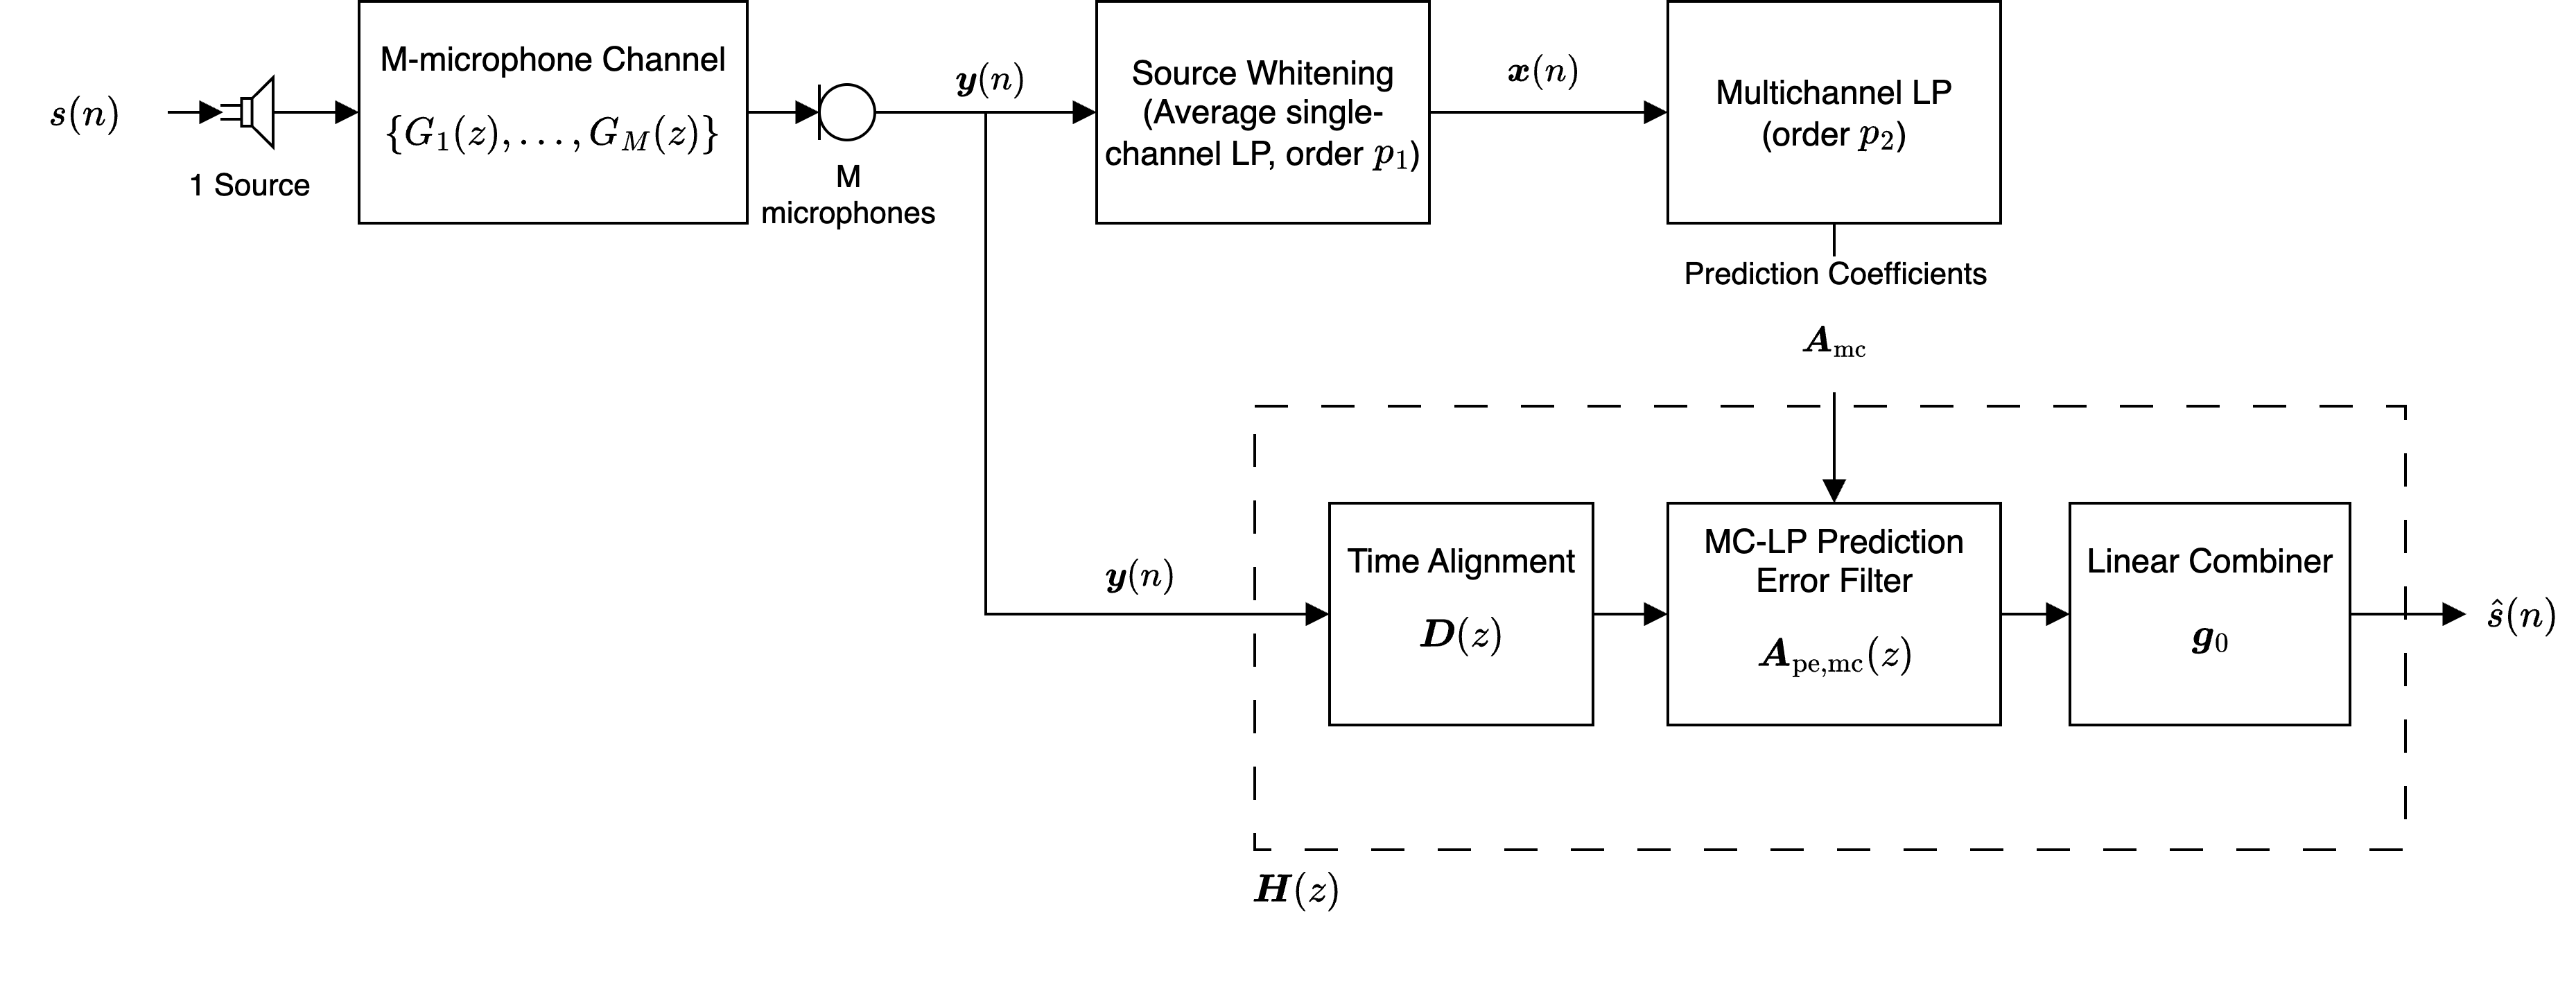
\includegraphics[width = 1.0\textwidth]{dap_block_diagram}
	\centering
	\caption[Block diagram for delay-and-predict dereverberation]{Block diagram for delay-and-predict dereverberation}
	\label{fig:dap_block_diagram}
\end{figure}


This approach consists of three stages:

\begin{enumerate}
	\item Source Whitening Stage: The AR parameters of the source are estimated and the corresponding prediction error filter is applied to each of the reverberant microphone signals, $\{y_1(n), \dots, y_M(n)\}$ (i.e., vector-valued $\boldsymbol{y}(n)$), thus whitening only the AR properties of the source. The result is a set of ``source-whitened" reverberant microphone signals, $\{x_1(n), \dots, x_M(n)\}$ (i.e., vector-valued $\boldsymbol{x}(n)$).
	%
	\item Multichannel Linear Prediction Stage: The source-whitened reverberant microphone signals are used in the multichannel Yule-Walker eqution (Equation \ref{eq:mc_yule_walker}) to compute the multichannel prediction coefficients, $\boldsymbol{A}_{\mathrm{mc}}$, and generate a multichannel prediction error filter, $\boldsymbol{A}_{\mathrm{pe,mc}}(z)$.
	%
	\item Dereverberation Stage: The multichannel prediction error filter from step 2 is combined in series with a time-alignment filter and a linear combiner to form the full delay-and-predict equalizer, $\boldsymbol{H}(z)$, which is applied to the original reverberant microphone signals, $\boldsymbol{y}(n)$. Since this prediction error filter was computed using the source-whitened signals, it should not include the AR parameters of the source signal, and thus should not whiten the source part of the microphone signals. Therefore the resulting prediction error signal should only whiten the channel, thus fascilitating dereverberation.
\end{enumerate}

In the source whitening stage, the AR parameters of the source are estimated as those that minimize the single-channel prediction error for all $M$ microphone signals. This is formulated as minimizing the sum of the single-channel prediction errors, i.e., the cost function is

\begin{equation}
	J = \sum_{m=1}^{M} E[ e_m^2(n) ] = \sum_{m=1}^{M} E[ y_m(n) - \sum_{k=1}^{p_1} \alpha_{s,k} y_m(n-k) ]
\end{equation}

Minimization of $J$ (i.e., setting $\frac{\partial J}{\partial \alpha_{s,k}} = 0$), assuming the microphone signals are stationary, the resulting normal equations are

\begin{eqnarray}
	\begin{bmatrix}
		\bar{r}_{yy}(0) & \bar{r}_{yy}(1) & \dots & \bar{r}_{yy}(p_1-1) \\
		\bar{r}_{yy}(1) & \bar{r}_{yy}(0) & \dots & \bar{r}_{yy}(p_1-2) \\
		\vdots               & \vdots              & \ddots & \vdots \\
		\bar{r}_{yy}(p_1-1) & \bar{r}_{yy}(p_1-2) & \dots & \bar{r}_{yy}(0)
	\end{bmatrix}
	\begin{bmatrix}
		\alpha_{s,1} \\
		\alpha_{s,2}  \\
		\vdots \\
		\alpha_{s,p_1}
	\end{bmatrix} =
	\begin{bmatrix}
		\bar{r}_{yy}(1)  \\
		\bar{r}_{yy}(2)  \\
		\vdots \\
		\bar{r}_{yy}(p_1) 
	\end{bmatrix} \\
	\boldsymbol{R}_{\mathrm{avg}} \boldsymbol{\alpha}_s = \boldsymbol{r}_{\mathrm{avg}} \label{eq:dap_source_whitening_yule_walker}
\end{eqnarray}

\noindent
where

\begin{equation}
	\bar{r}_{yy}(l) = \sum_{m=1}^{M} r_{y_m y_m}(l) = \sum_{m=1}^{M} E[ y_m(n) y_m(n-l) ] \label{eq:dap_avg_autocorr}
\end{equation}

\noindent
i.e., $\bar{r}_{yy}(l)$ is the average autocorrelation accross all microphones. Thus the source-whitening stage blindly estimates the AR parameters of the source by smoothing autocorrelation values accross spatial sampling points to effectivelty average out the effects of the RTFs which are assumed not to have common AR parameters.

The resulting single-channel prediction error filter (i.e., the source-whitening filter), $A_s(z)=1-\sum_{k=1}^{p_1}\alpha_{s,k}z^{-k}$, is applied to the reverberant microphone signals to get the source-whitened reverberant signals, $\boldsymbol{x}(n)$, i.e., $\boldsymbol{x}(n)=\boldsymbol{y}(n) - \sum_{k=1}^{p_1}\alpha_{s,k}\boldsymbol{y}(n-k)$.

In the multichannel linear prediction stage, the multichannel Yule-Walker equations (Equation \ref{eq:mc_yule_walker}) are solved using the source-whitened signals, i.e.,

\begin{equation}
	\boldsymbol{A}_{\mathrm{mc}} = \boldsymbol{r}_{\mathrm{mc}} \boldsymbol{R}_{\mathrm{mc}}^{-1} \label{eq:dap_mc_lp_yule_walker}
\end{equation}

\noindent
with $\boldsymbol{R}_{\mathrm{mc}} = E[\boldsymbol{\tilde{x}}(n) \boldsymbol{\tilde{x}}^T(n)]$, $\boldsymbol{r}_{\mathrm{mc}} = E[\boldsymbol{x}(n)\boldsymbol{\tilde{x}}^T(n-1)]$, and \newline $\boldsymbol{\tilde{x}}(n) = \begin{bmatrix} \boldsymbol{x}^T(n) &	\boldsymbol{x}^T(n-1)  & \dots  & \boldsymbol{x}^T(n-p_2+1) \end{bmatrix}^T$. The resulting multichannel prediction error filter is $\boldsymbol{A}_{\mathrm{mc}}(z) = \boldsymbol{I} - \sum_{k=1}^{p_2} \boldsymbol{A}_k z^{-k}$.


In the dereverberation stage, the actual multichannel equalizer filter, $\boldsymbol{H}(z)$, is computed as 

\begin{equation}
	\boldsymbol{H}(z) = \boldsymbol{g}_0 \boldsymbol{A}_{\mathrm{pe,mc}}(z) \boldsymbol{D}(z)
\end{equation}

\noindent
where $\boldsymbol{D}(z)$ is a diagonal matrix of delay elements ($\boldsymbol{D}(z) = \mathrm{diag} \{z^{-d_1} \dots z^{-d_M}\}$) used to time-align the microphone signals, and $\boldsymbol{g}_0$ is a weighting vector that computes a linear combination of the length-$M$ vector output of the multichannel prediction error filter. Together $D(z)$ and $\boldsymbol{g}_0$ effectively perform delay-weight-and-sum beamforming on the equalized vector output of the multichannel prediction error filter. To generate $\boldsymbol{D}(z)$, the time delay between the microphones must be estimated, which is a well understood topic with many practical approaches. In the original DAP algorithm, the linear combiner weights $\boldsymbol{g}_0$ were selected to be the vector coefficient of the SIMO channel, i.e., $\boldsymbol{g}_0 = \begin{bmatrix} g_1(0) \dots g_M(0) \end{bmatrix} ^T$. It was shown that $\boldsymbol{g}_0$ can be blindly estimated with reasonable accuracy as the eigenvector corresponding to the largest eigenvalue of the autocorrelation matrix corresponding to the multichannel prediction error signal from the second algorithm stage, $\boldsymbol{e}_{\boldsymbol{x}}(n)$, i.e., $\boldsymbol{g}_0$ is estimated as the principal component of the matrix $\boldsymbol{R}_{\boldsymbol{e}_{\boldsymbol{x}}(n) \boldsymbol{e}_{\boldsymbol{x}}(n)} = E[\boldsymbol{e}_{\boldsymbol{x}}(n) \boldsymbol{e}^T_{\boldsymbol{x}}(n) ]$, where

\begin{equation}
	\boldsymbol{e}_{\boldsymbol{x}}(n) = \boldsymbol{x}(n) - \hat{\boldsymbol{x}}(n) = \boldsymbol{x}(n) - \sum_{k=1}^{p_2} \boldsymbol{A}_k \boldsymbol{x}(n-k)
\end{equation}

The final output of the DAP equalizer is thus computed as 

\begin{equation}
	\hat{S}(z) = \boldsymbol{H}(z) \boldsymbol{y}(z)  \label{eq:dap_eq_output}
\end{equation}

\noindent
or equivalently

\begin{equation}
	\hat{s}(n) = \sum_{m=1}^{M} g_m(0) \hat{s}_m(n-d_m) \\
\end{equation}

\noindent 
with

\begin{equation}
	\begin{bmatrix} \hat{s}_1(n-d_1) \\ \dots \\ \hat{s}_M(n-d_M) \end{bmatrix} =
	\boldsymbol{y}(n) - \sum_{k=1}^{p_2} A_k \boldsymbol{y}(n-k)
\end{equation}

\cite{triki2006delay} explained that the prediction order for the multichannel linear prediction stage ($p_2$) should be selected such that it meets the MINT requirements, i.e., $p_2=L_g/(M-1)$, where $L_g$ is the length of the FIR channels. It was suggested that the prediction order for the source-whitening stage ($p_1$) should be selected such that that the source is sufficiently undistorted by the multichannel prediction error filter. For a sample rate of \qty{8}{\kilo\hertz}, $p_1=100$ was considered sufficient. However, it should be noted that the higher order AR parameters of the source (i.e., higher than those reflected by $p_1$) will still be included in the multichannel prediction error filter, distorting the estimate of the true system inverse, which will limit its applicability to other source signals.

Additionally, note that the source signal does not need to be stationary (only long-term stationary), but rather it is only important that the same window of speech is used in the estimation of the source AR parameters and the multichannel prediction coefficients. As such, it was recommended that the entire speech stimulus be used in analysis so as to reduce estimation variance.

As per the MINT, DAP requires that the RTFs have no common zeros, and have the additional requirement that the AR parameters of the channels (i.e., the effective poles) do not overlap. If the effective poles of the RTFs overlap, these will be wrongly associated with the source and will not be equalized. As channel order increases (i.e., longer reverberation times), the concentration of zeros around the unit circle increases and the likelihood of overlapping or numerically overlapping zeros increases, thus requiring more microphones to acheive reasonable performance. 

When formulated as MIMO prediction of signal vector $\boldsymbol{y}(n)$ (i.e., as in Equation \ref{eq:mc_lp_error_parallel}), there is potential to constrain the solution so that the phase of the individual dereverberated signals in $\boldsymbol{e}(n)$ are not distorted. In this way the output of the algorithm can be input to further spatial processing and/or spatial cues can be preserved to aid in speech perception (Section \ref{perceptual_adaptations}).

\noindent
\newline
\textbf{LIME and other MC-LP-Based Dereverberation Algorithms} \label{section:other_mc_lp_approaches}

\noindent
In the linear-predictive multiple-input equalizatino (LIME) dereverberation algorithm, the multichannel prediction coefficients are estimated directly from the reverberant microphone signals, $\{y_1(n), \dots, y_M(n)\}$. The multichannel prediction error filter thus whitens the source signal, and then an un-whitening filter is applied after. \cite{delcroix2007precise}, showed that under a certain matrix formulation, the multichannel prediction coefficients corresponding to the reverberant microphone signals and the source AR parameters can be independently extracted.

Several extensions of DAP and LIME have been proposed, such as methods for compensating the effects of additive noise \citep[e.g., ][]{triki2007multivariate}, alternative methods for combining the $M$ dereverberated signals in $\boldsymbol{e}(n)$ \citep[e.g., ][]{triki2008robust}, and adaptive extensions which generally use RLS for adaptation and often operate in the FFT/subband domain \citep[e.g., ][]{jukic2016adaptive, jukic2016general}. Usage of delayed linear prediction \citep[i.e., multi-step linear prediction originally presented by ][]{gesbert1997robust} has also been proposed, whereby a multi-sample delay is applied to the signals being used in prediction instead of the traditional single-sample delay. Delayed linear prediction allows algorithms to avoid cancelling the early reflections and also reduces the over-whitening effects of linear prediction, but is more computationally complex. 

Multichannel linear predictive techniques are often considered to be the most practical approach to reverberation cancellation due to the fact they can be performed in a truly blind manner, not requiring any knowledge of the source or channel order, and since linear prediction is a well understood topic that is easily extensible to an adaptive framework. These approaches have generally proven to perform well for shorter reverberation times, but their performance diminishes with increased reverberation due to estimation variance and the massive amounts of data needed to reduce estimation variance. Additionally, the underlying assumption that RTFs are time-invariant severly limits performance in practice since real acoustics are highly time varying. For longer reverberation times, where channel orders can reach up to tens of thousands (e.g., a T60 of \qty{2}{\second} at a sample rate of \qty{16}{\kilo\hertz} represents an RIR of length \qty{32}{\kilo samples}), solving the normal equations also becomes impractical due to the massive matrices involved, and equalizers can introduce substantial delay. However, the computational cost can be reduced at the cost of decreased performance by using stochastic gradient descent algorithms which do not require matrix inversion.

To manage the performance limitations of these approaches, several authors have suggested the enhancement of multichannel linear predictive inverse filtering with a spectral subtraction post-processing stage to reduce residual late reflections \citep[e.g., ][]{furuya2007robust}. Some authors have also suggested using linear prediction to estimate reverberation, but then removing it via spectral subtraction rather than inverse filtering \citep[e.g., ][]{kinoshita2007multi, nakatani2008blind, nakatani2010speech}, claiming that this approach is more robust to imperfections in system estimate. 


\subsubsection{Blind System Identification Using Estimation Theory} \label{section:bsi_estimation_theory}

In recent years, significant research has gone into blind reverberation cancellation techniques that use statistical estimation methods for BSI. One of the most seminal approaches is the so-called weighted prediction error algorithm \citep[i.e., WPE ][]{nakatani2008blind, nakatani2010speech}, which is one of the most common algorithms applied in practice. In this multichannel method, the reverberant speech signal is conceptually divided into a ``desired" direct/early component and a late reverberant component, and an estimate of the late reverberant component is subtracted from the observed signal. A single reverberant microphone signal is modeled as a multichannel delayed linear-predictive process as a function of all microphone signals, with a prediction delay matching the defined boundary between early and late reflections. The desired component is modeled as a Gaussian process that is short-time quasi-stationary with time varying variance over longer time. The delayed prediction coefficients of the process are estimated via maximum likelihood estimation, and the resulting prediction error filter is used to subtract the late reflections. The technique was also extended to the STFT/subband domains to reduce computational complexity. The WPE algorithm is iterative and models speech as having time-varying variance, which allows it to track time-varying RTFs, and track/exploit time-varying speech statistics. The time-variant formulation of WPE generally has allowed it to outperform conventional MC-LP approaches such as DAP dereverberation.

A number of appraoches have also been proposed which setup Bayesian priors \citep[e.g., ][]{hopgood2005models}, with some priors more recently being based on the assumed sparsity of the time-frequency representation of clean speech \citep{jukic2015multi, jukic2016general}.

Several authors have also enhanced this concept with techniques for modeling the time-varying nature of the acoustics. This has been done by treating the prediction coefficients (i.e., the model parameters) themselves as random variables with parameters to be estimated. Parameter estimation in this case has been proposed primarily using recursive estimation procedures such as Kalman filtering \citep[e.g., ][]{braun2016online, schmid2014variational}. The simplest example of such a model is the so-called random-walk time-varying all-pole system, where individual poles are modeled as having Gaussian variation about their true value/mean. The ability of a probablistic framework to include modeling of the time-varying nature of acoustic represents a major potential benefit of these appraoches. Similarly, the clean speech source signal can be assigned a source-filter model, and the time-varying vocal tract can be modeled probablistically \citep{grenier2003time}. In this way the time-varying nature of speech can be leveraged rather than simply modeling the long-term statistics of speech as is done in non-probablistic approaches. Since a noise model can also be included in the setup, probablistic approaches tend to be less sensitive to noise.
 
Probablistic methods for estimating the clean speech and/or channel generally tend to outperform traditional inverse filtering approaches such as delay-and-predict/LIME dereverberation, especially in non-stationary reverberation. Although these approaches are incredibly computationally complex, simplified (lower-order) configurations and online variants have made their way into many practical applications.

\section{Summary and Thesis Goals}

The previous two chapters outlined the perceptual motivation for dereverberation, and existing dereverberation algorithms. It was discussed that beamforming and statistical speech enhancement methods for reverberation suppression have proven to be computationally efficient and practical approaches to reducing the perceptual impacts of reverberation. However, due to their simplicity and limitations in their formulation, their performance is somewhat limited, and the often distort speech (e.g., musical noise). On the other hand, multichannel reverberation cancellation methods have potential to perfectly remove reverberation without distorting the source signal as dictated by the MINT, but their performance at long reverberation times is limited, especially in non-stationary/noisy environments due to the underlying BSI problem. Several MC-LP-based approaches were discussed, including the delay-and-predict (DAP) algorithm \citep{triki2006delay} which is based on traditional solving of the multichannel Yule-Walker equations, and the more recent weighted prediction error (WPE) algorithm \citep{nakatani2008blind, nakatani2010speech} which extended this concept to a estimation theory framework and has proven to be one of the most practical approaches. It was discussed that MC-LP methods (and in particular delayed-MC-LP methods) to BSI show the most promise, but still perform poorly for later weak reflections, and solving the underlying normal equations (or solving complex MLE solution in statistical estimation variants) represents a massive computational cost. As such, many practical/effective approaches to dereverberation use multichannel linear predictive blind deconvolution to cancel the strong early part of the RIR, and are enhanced with statistical speech enhancement post-processing to suppress the diffuse/weak late tail of the RIR.

The goal set for this thesis was to provide a physiologically motivated perceptual analysis of the performance of MC-LP approaches to reverberation cancellation under practical conditions. For a case study, the delay-and-predict algorithm was implemented and parameter-tuned for efficacy (Chapter 3), and its performance was assessed (Chapter 4). 
        \setcounter{figure}{0}
        \setcounter{equation}{0}
        \setcounter{table}{0}


\chapter{Delay and Predict Dereverberation Parameters}

The goal of this chapter was to analyze the influence of the various algorithm parameters and signal properties on the performance of the delay-and-predict (DAP) dereverberation algorithm, and tune them accordingly for the following chapter. The parameters/properties that were analyzed are:

\begin{enumerate}
	\item \textbf{Multichannel Linear Prediction Order} ($p_2$): The filter order used in the multichannel linear prediction stage, i.e., the order of the multichannel prediction error filter, $\boldsymbol{A}_{\mathrm{pe,mc}}(z)$. Note that this refers to the prediction order in a vector-valued sense, so it is the order of the individual FIR filters applied to each microphone signal.
	%
	\item \textbf{Source Whitening Linear Prediction Order} ($p_1$): The filter order used to pre-whiten the source spectrum before the multi-channel linear prediction stage.
	%
	\item \textbf{Source Data Length}: The amount of signal data used in computation of both the source-whitening prediction coefficients and the multichannel linear prediction coefficients
	%
	\item \textbf{Source Spectrum}: The degree of colouration in the source signal. I.e., the properties of the source which must be pre-whitened by the source-whitening stage (i.e., for algorithm training).
	%
	\item \textbf{Time Alignment of RIRs}: How well aligned the microphone signals were before computation of the multichannel linear prediction coefficents. I.e., the influence of the diagonal matrix-valued time-delay filter, $\boldsymbol{D}(z)$.
	%
	\item \textbf{Linear Combiner} ($\boldsymbol{g}_0$): The impact of computing the final dereverberated signal by linearly combining the $M$ individual dereverberated signals (i.e., linear combination of the dereverberated vector-valued signal).
\end{enumerate}

\section{Multichannel Linear Prediction Order} \label{section:params_p2} 

\subsection{MINT Inverse Filtering Results} \label{section:params_p2_MINT} 

Neglecting the performance impact of blind RTF estimation, the MINT (Section \ref{MINT}) dictates that it is theoretically possible to perfectly invert the room response captured at multiple microphones, provided the channels do not contain common zeros, and the individual FIR equalizer filters are of length $\left(p_2+1\right) >= \left(L-1\right) / \left(M-1\right)$, where $L$ is the length of the individual FIR RIRs and $M=4$ is the number of microphones. To be confirm this, the MINT was implemented and applied to a set of known RIRs over a range of values for $p_2$. The four RIRs used in this comparison were real RIR measurements taken from the "SAL" room that is part of the MYRiAD database \citep{dietzen2023myriad} (discussed in more detail in Section \ref{sec:rir_databases}). The T60 of the original RIRs was \qty{2.1}{\sec}, but this was synthetically reduced to \qty{100}{\milli\sec} by applying an exponentially decaying window. This exponential truncation method is described in more depth in Section \textbf{TODO... Maybe explain it here actually}. The equalized impulse responses (EIR) was generated by passing the filtering and summing the RIRs of the $M$ channels with the DAP equalizer (Equation \ref{eq:dap_eq_output}), and the corresponding energy decay curve (EDC) was generated from the EIR via Equation \ref{eq:edc}. The EIR and EDC for each MINT filter order is shown in Figure \ref{fig:params_p2_MINT_compare}.

As expected, near-perfect equalization was acheived by the MINT for $p2 = L / \left(M-1\right)$, with the EDC decaying by $>$ \qty{250}{\decibel} (Figure \ref{subfig:params_p2_MINT_compare:A}) almost instantaneously. Similarly, when the T60 was used to set the equalizer length rather than the actual FIR RIR length, the EDC decayed by about approximately 60 dB almost instaneously (Figure \ref{subfig:params_p2_MINT_compare:B}). As the equalizer length was decreased relative to the T60, the EDC performance of the MINT dropped substantially. Based on these observations, The $p_2$ should be selected such that it is possible to acheive the amount of attenuation desired. If the goal is to reduce the T60, $p_2 = \mathrm{N60}  / \left(M-1 \right)$ is sufficient.


\begin{figure}[H]
	\centering
	
	% ROW A
	\makebox[\textwidth][l]{%
		\begin{minipage}{0.23\textwidth}
			\centering
			\raggedleft{\footnotesize \textbf{(a)} \newline $p_2 = L / (M-1)$} \\
		\end{minipage}%
		\begin{minipage}{0.675\textwidth}
			\begin{subfigure}[t]{0.49\textwidth}
				\centering
				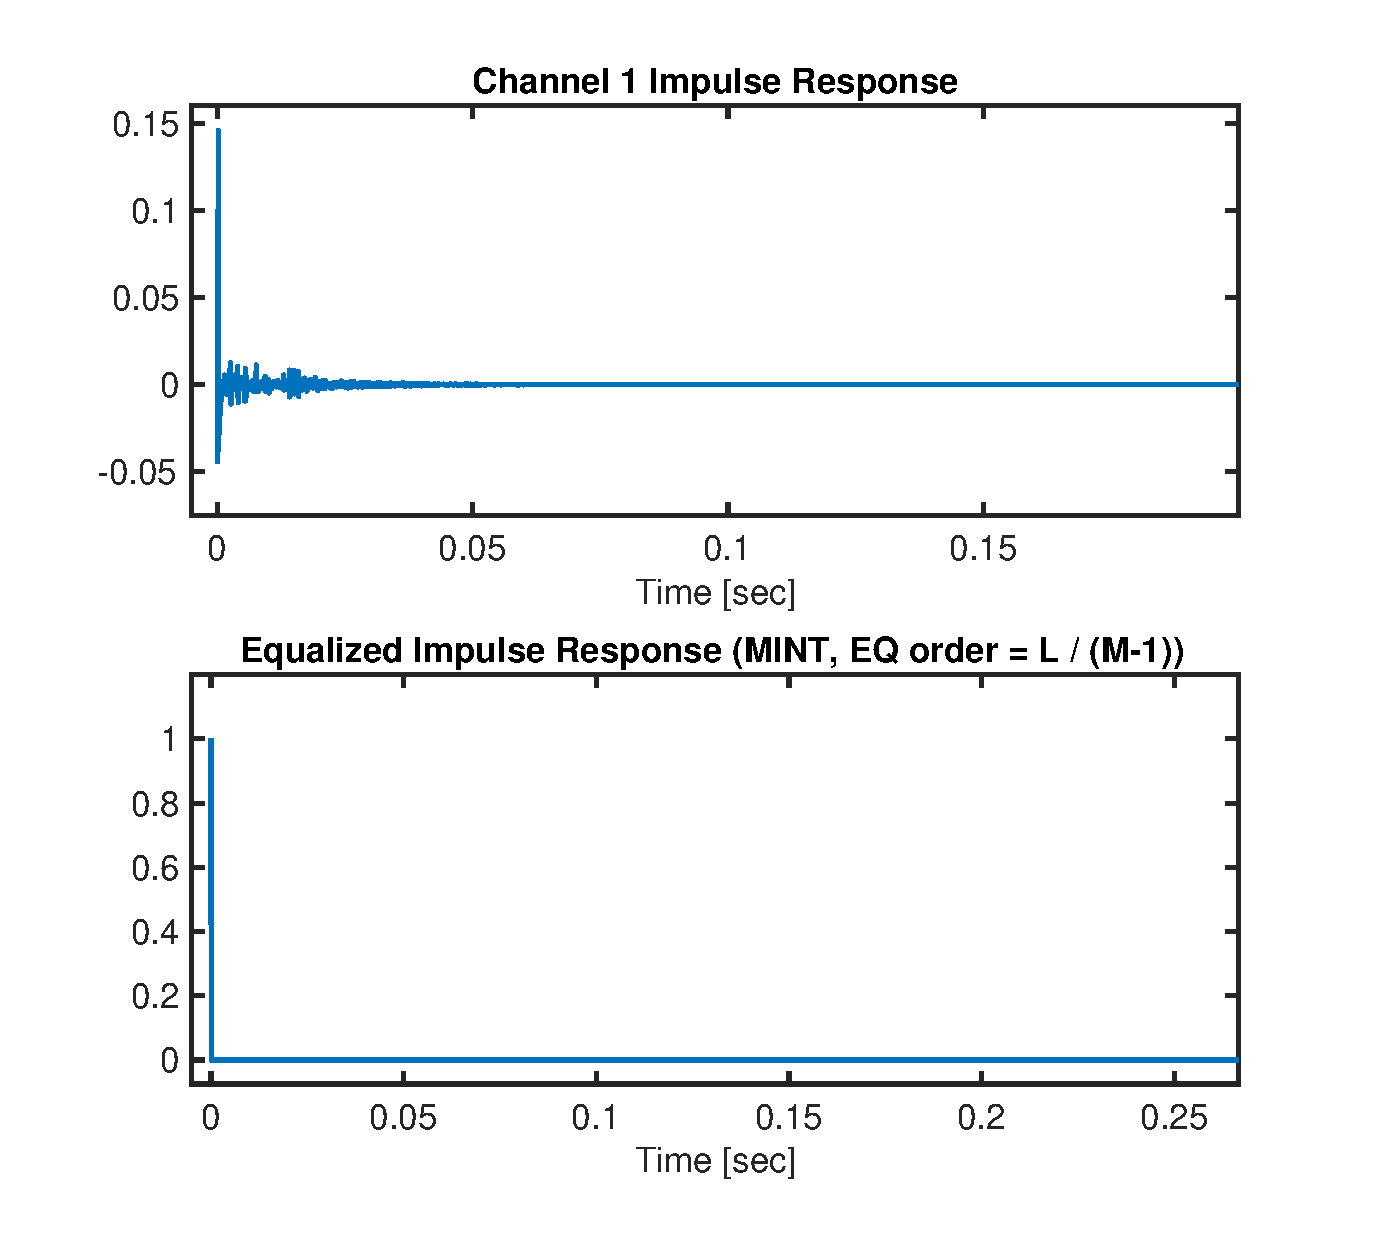
\includegraphics[width=\linewidth]{MINT_EIR_L_div_M_minus_1}
			\end{subfigure}
			\hfill
			\begin{subfigure}[t]{0.49\textwidth}
				\centering
				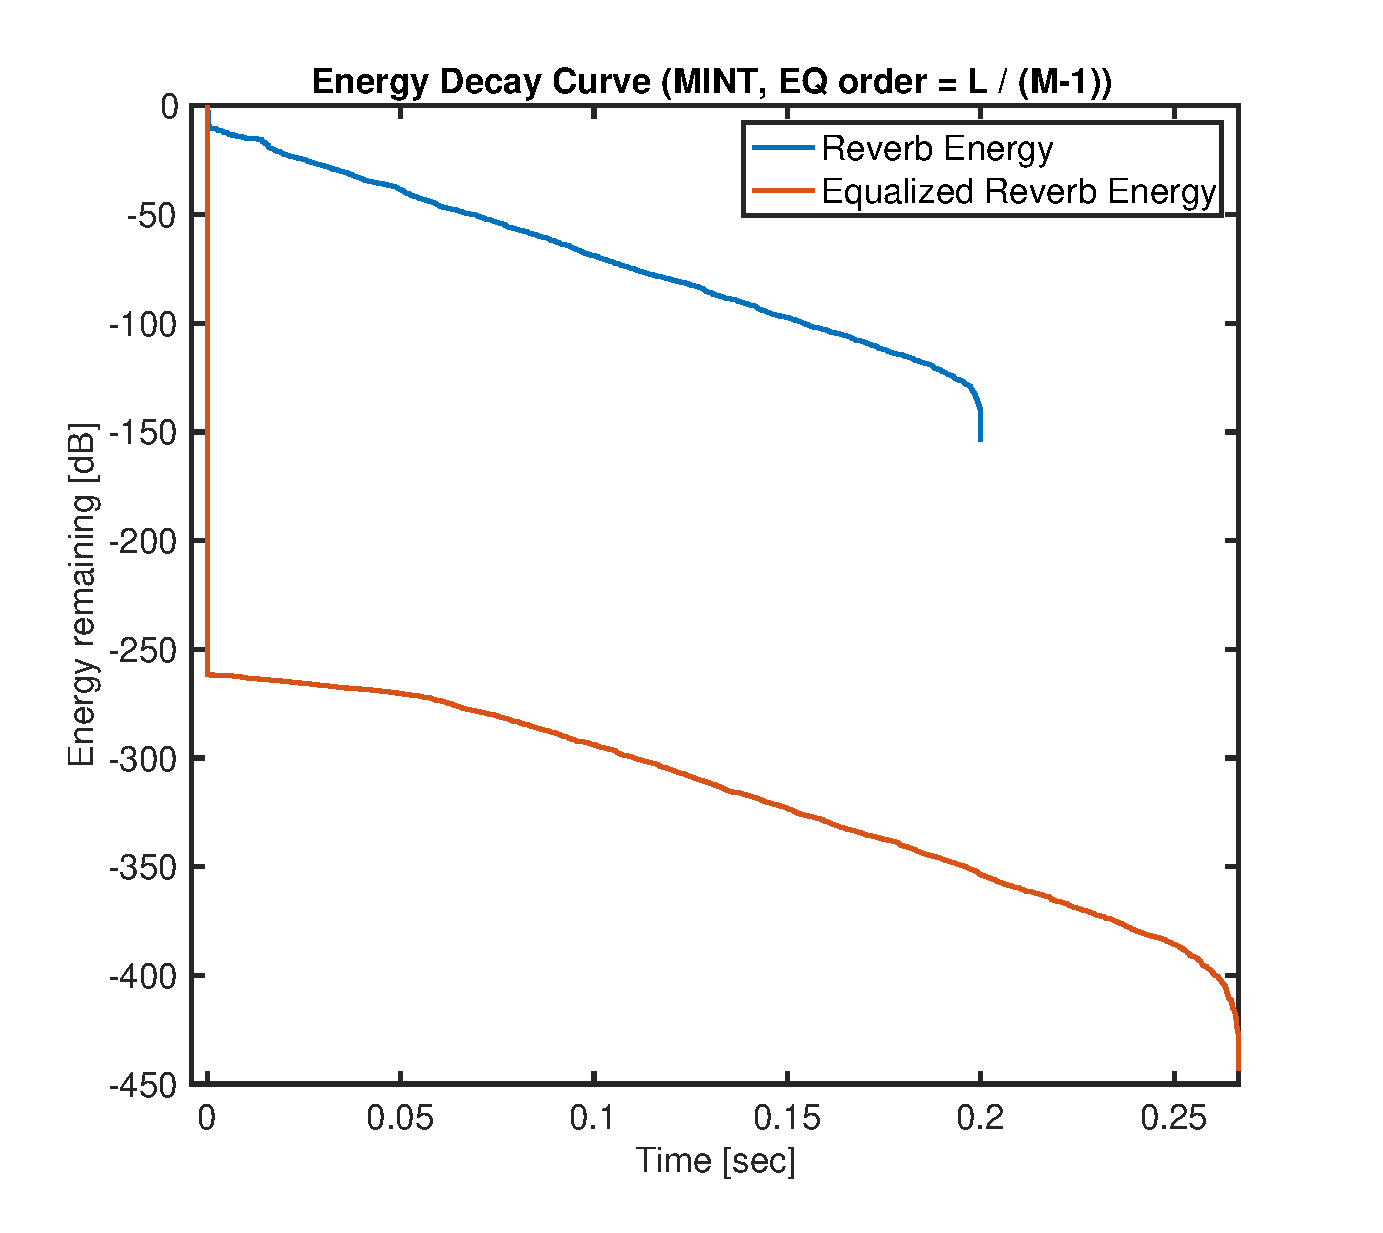
\includegraphics[width=\linewidth]{MINT_EDC_L_div_M_minus_1}
			\end{subfigure}
		\end{minipage}
	}
	% Dummy subfigure for referencing row A
	\refstepcounter{subfigure}
	\label{subfig:params_p2_MINT_compare:A}
	
	\vspace{1em}
	
		% ROW B
	\makebox[\textwidth][l]{%
		\begin{minipage}{0.23\textwidth}
			\centering
			\raggedleft{\footnotesize \textbf{(b)} \newline $p_2 = \mathrm{N60}  / (M-1)$} \\
		\end{minipage}%
		\begin{minipage}{0.675\textwidth}
			\begin{subfigure}[t]{0.49\textwidth}
				\centering
				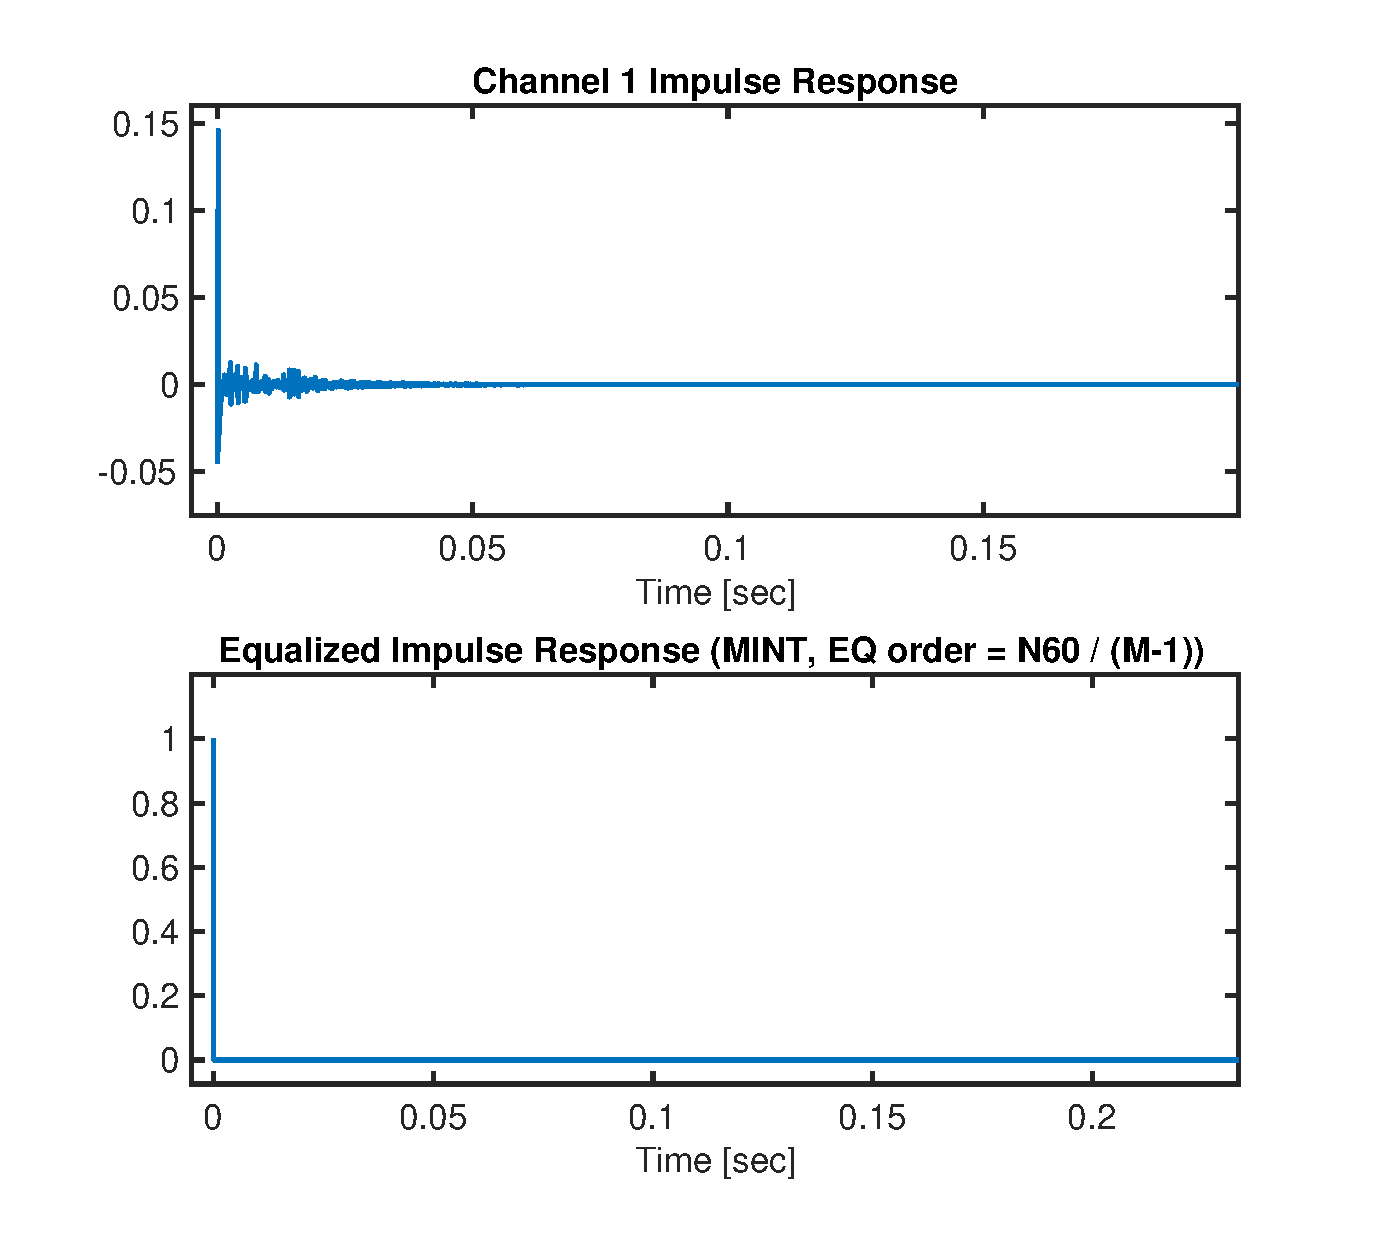
\includegraphics[width=\linewidth]{MINT_EIR_N60_div_M_minus_1}
			\end{subfigure}
			\hfill
			\begin{subfigure}[t]{0.49\textwidth}
				\centering
				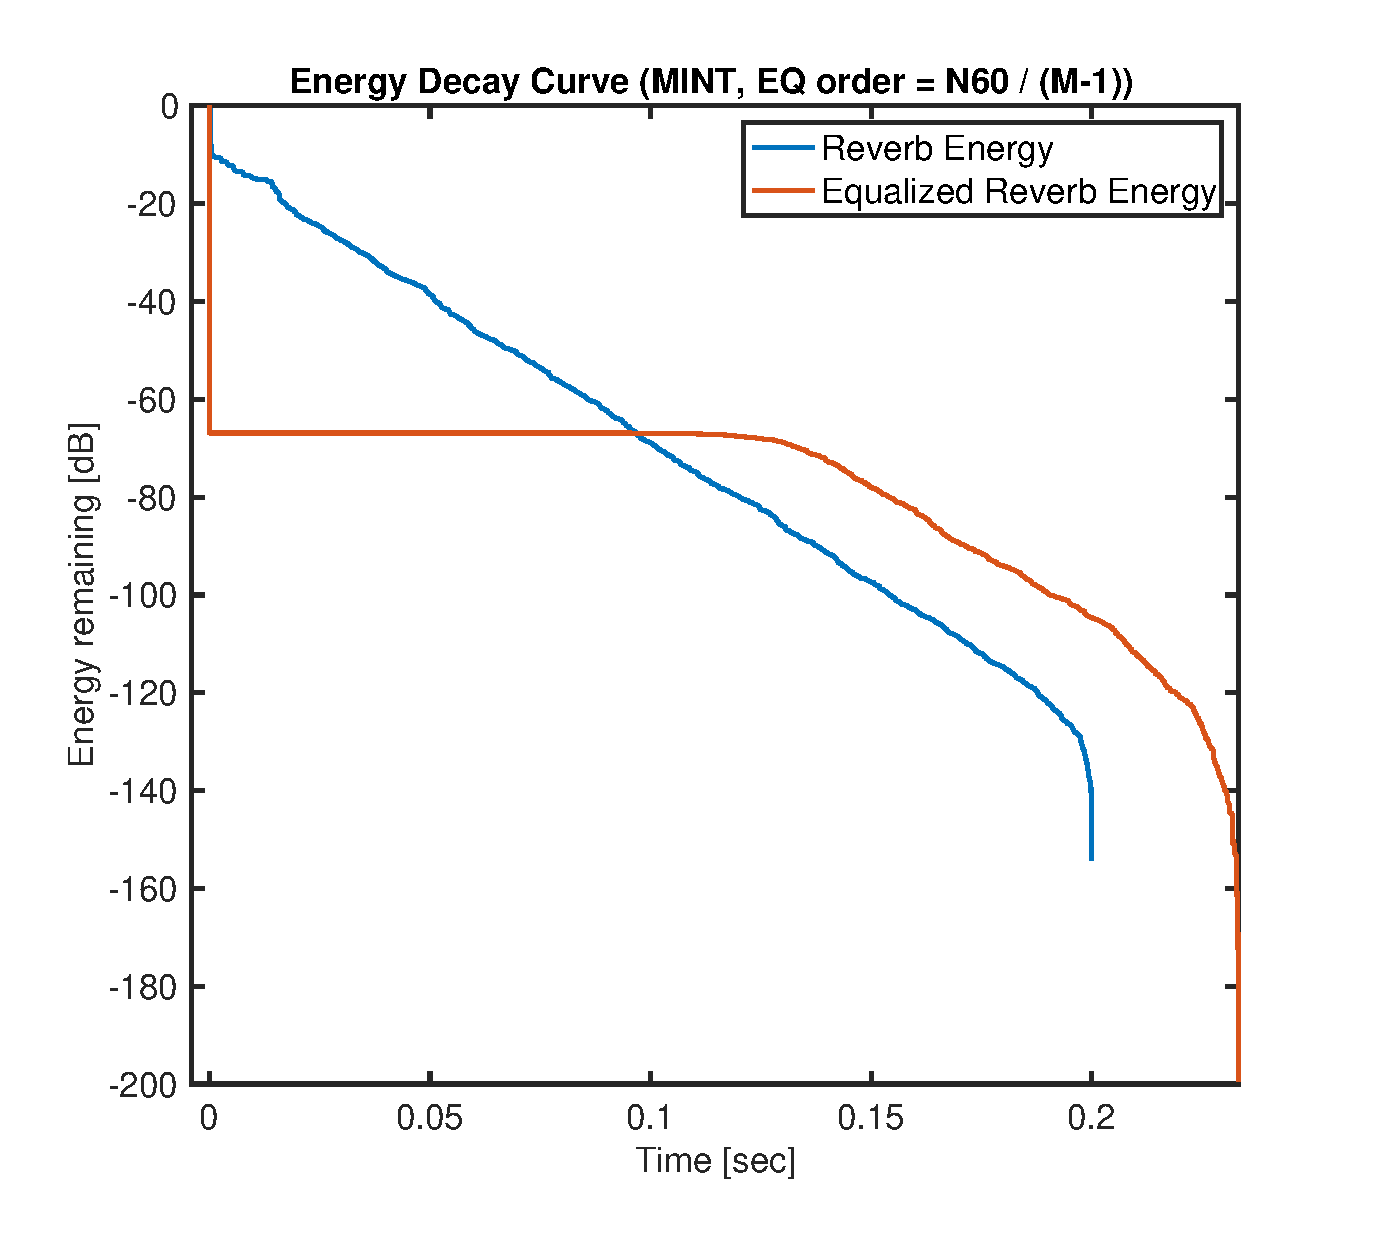
\includegraphics[width=\linewidth]{MINT_EDC_N60_div_M_minus_1}
			\end{subfigure}
		\end{minipage}
	}
	% Dummy subfigure for referencing row B
	\refstepcounter{subfigure}
	\label{subfig:params_p2_MINT_compare:B}
	
	\vspace{1em}
	
		% ROW C
	\makebox[\textwidth][l]{%
		\begin{minipage}{0.23\textwidth}
			\centering
			\raggedleft{\footnotesize \textbf{(c)} \newline $p_2 = 0.75 \cdot \mathrm{N60}  / (M-1)$} \\
		\end{minipage}%
		\begin{minipage}{0.675\textwidth}
			\begin{subfigure}[t]{0.49\textwidth}
				\centering
				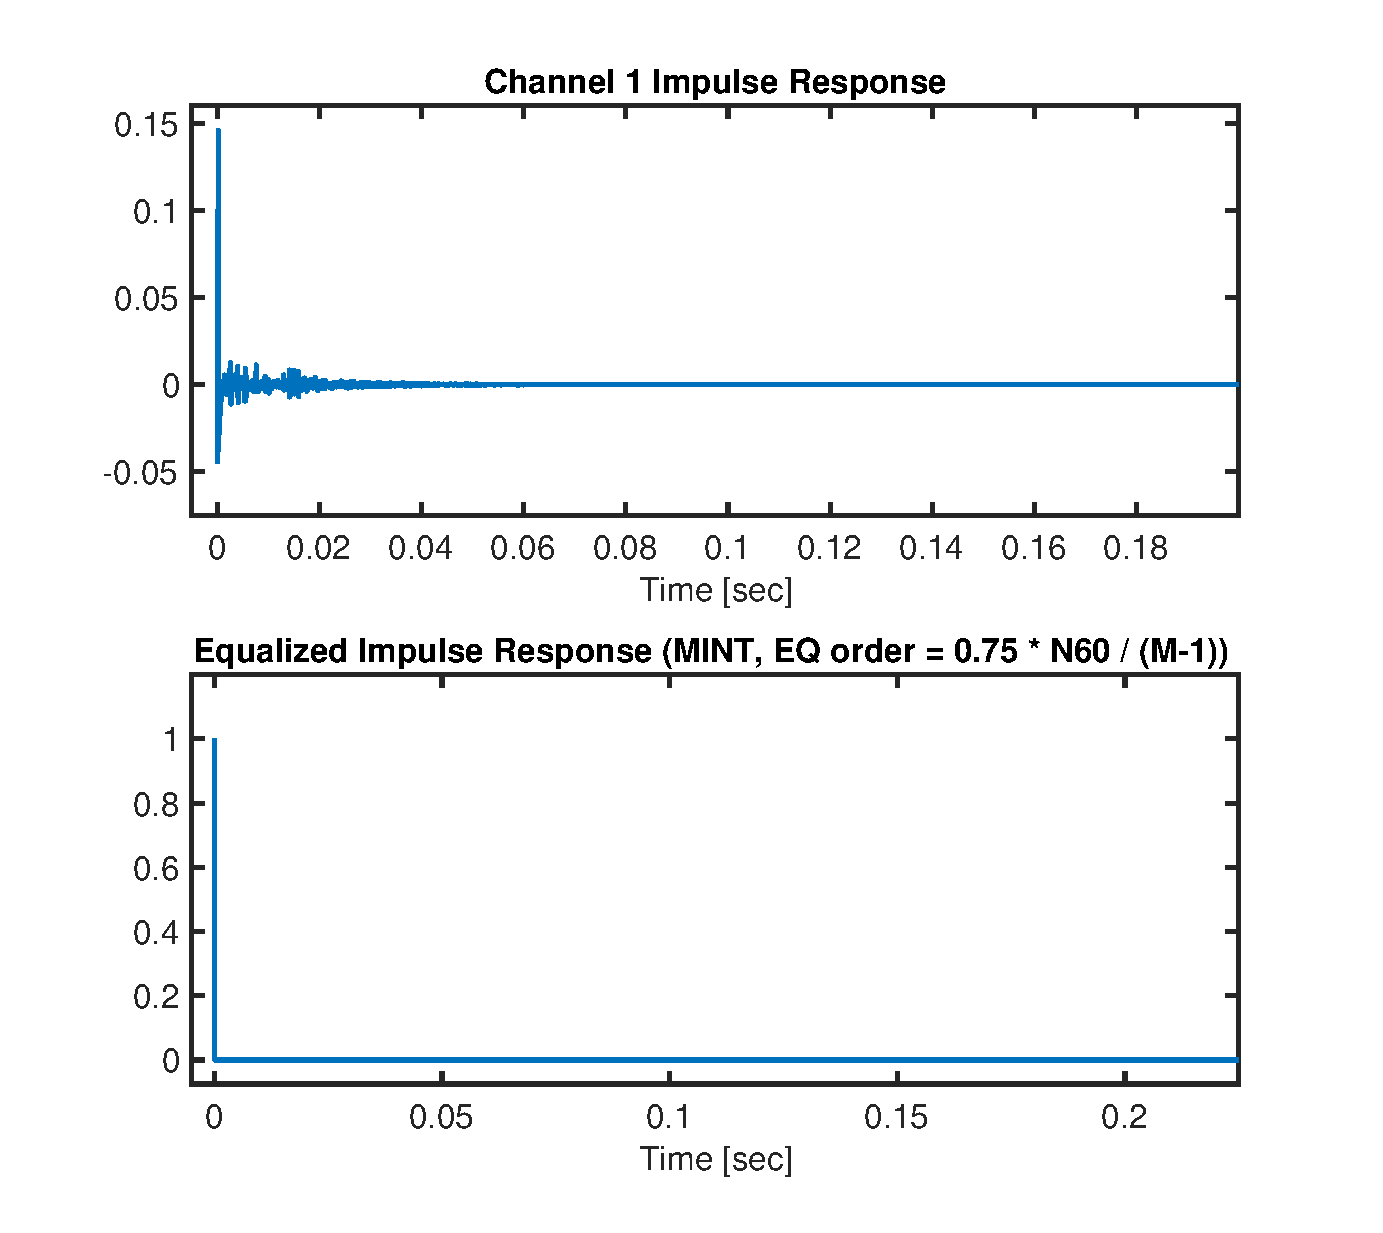
\includegraphics[width=\linewidth]{MINT_EIR_0p75N60_div_M_minus_1}
			\end{subfigure}
			\hfill
			\begin{subfigure}[t]{0.49\textwidth}
				\centering
				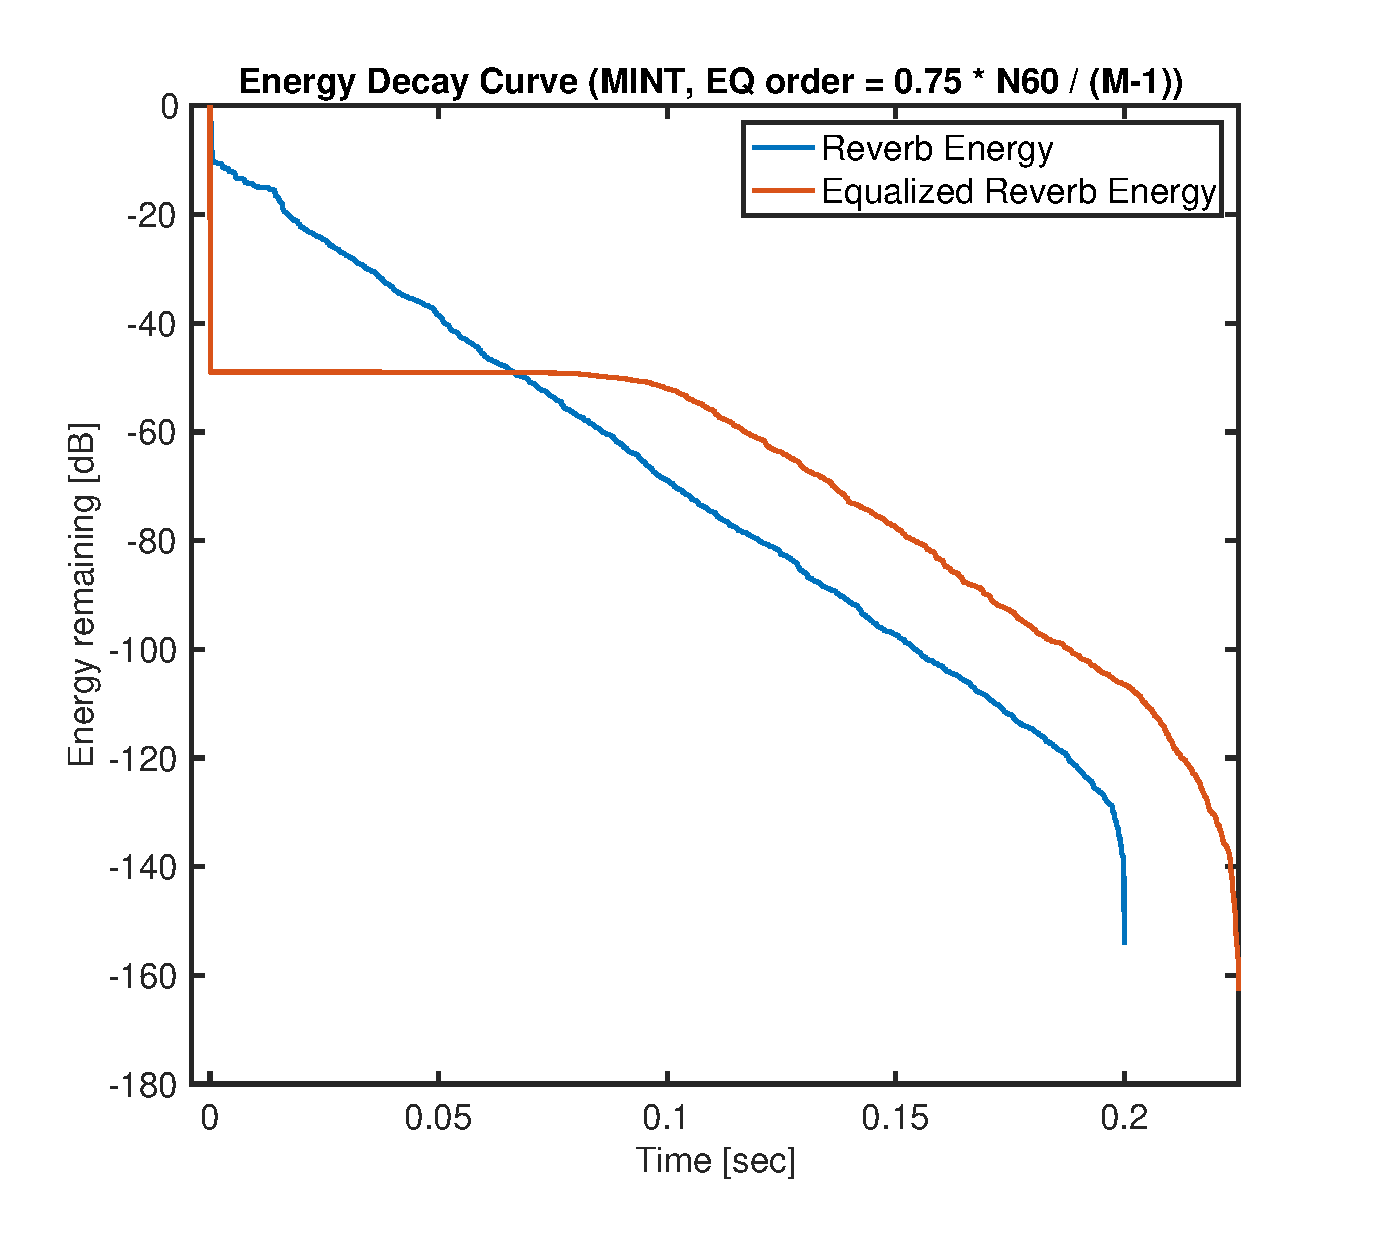
\includegraphics[width=\linewidth]{MINT_EDC_0p75N60_div_M_minus_1}
			\end{subfigure}
		\end{minipage}
	}
	% Dummy subfigure for referencing row C
	\refstepcounter{subfigure}
	\label{subfig:params_p2_MINT_compare:C}
	
	\vspace{1em}
	
		% ROW D
	\makebox[\textwidth][l]{%
		\begin{minipage}{0.23\textwidth}
			\centering
			\raggedleft{\footnotesize \textbf{(d)} \newline $p_2 = 0.5 \cdot \mathrm{N60} / (M-1)$} \\
		\end{minipage}%
		\begin{minipage}{0.675\textwidth}
			\begin{subfigure}[t]{0.49\textwidth}
				\centering
				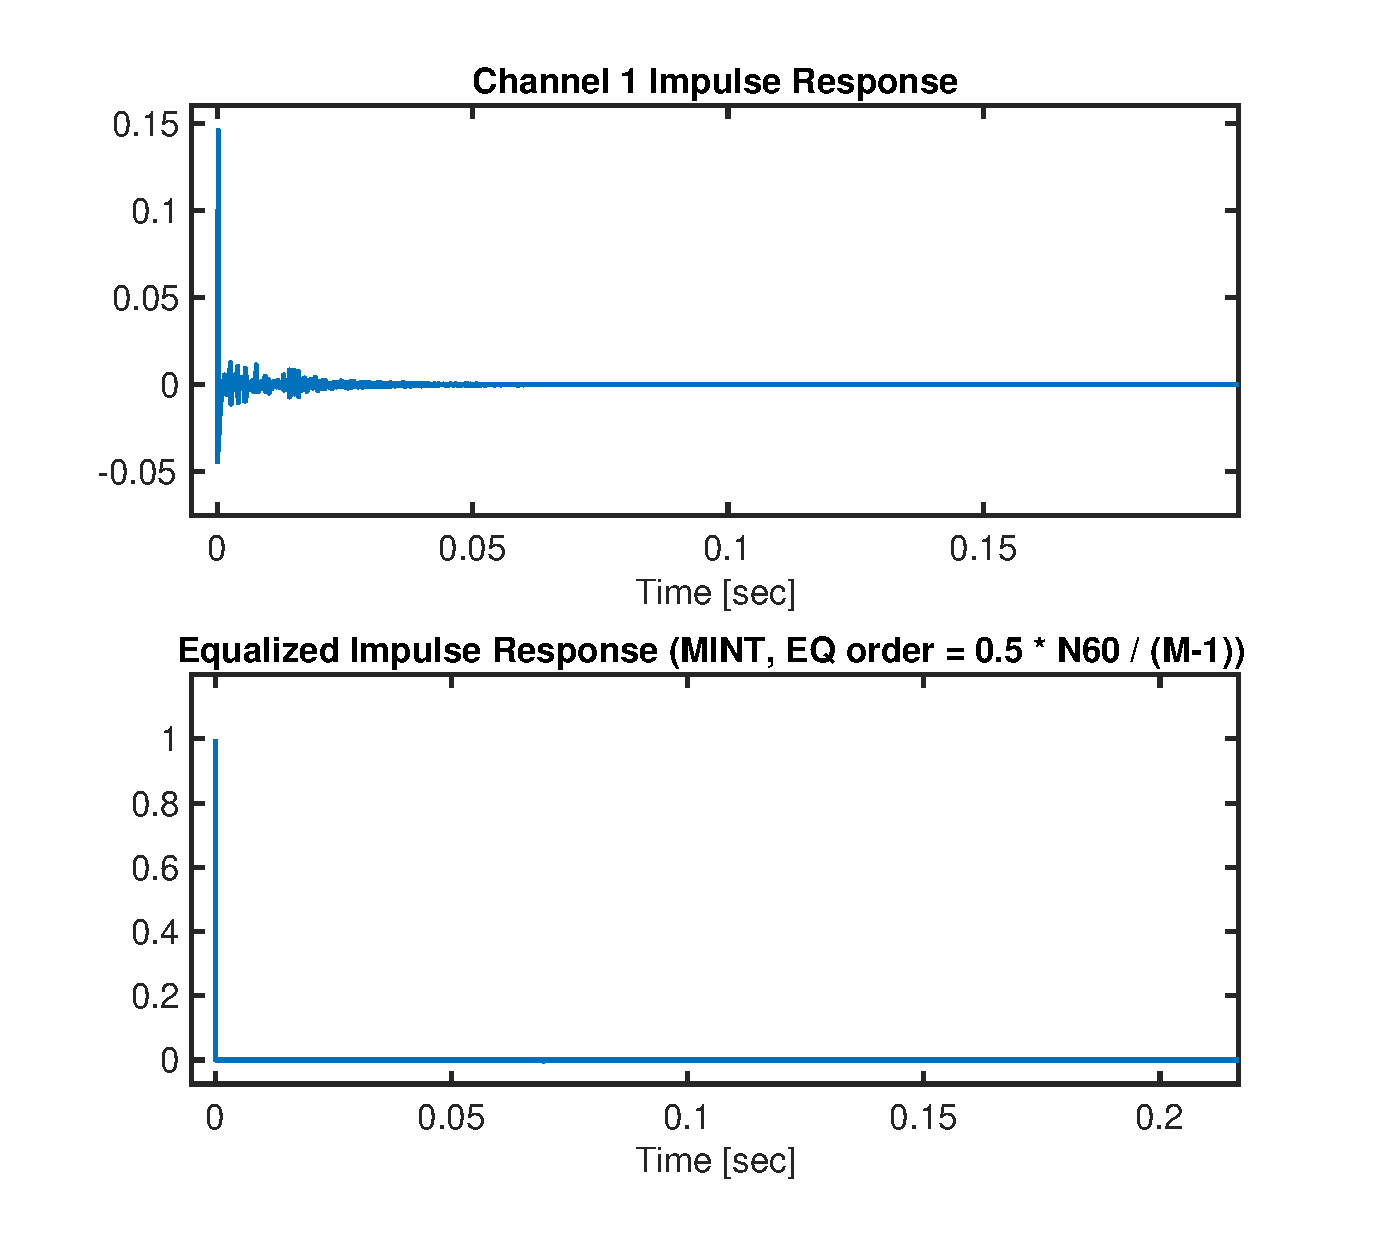
\includegraphics[width=\linewidth]{MINT_EIR_0p5N60_div_M_minus_1}
			\end{subfigure}
			\hfill
			\begin{subfigure}[t]{0.49\textwidth}
				\centering
				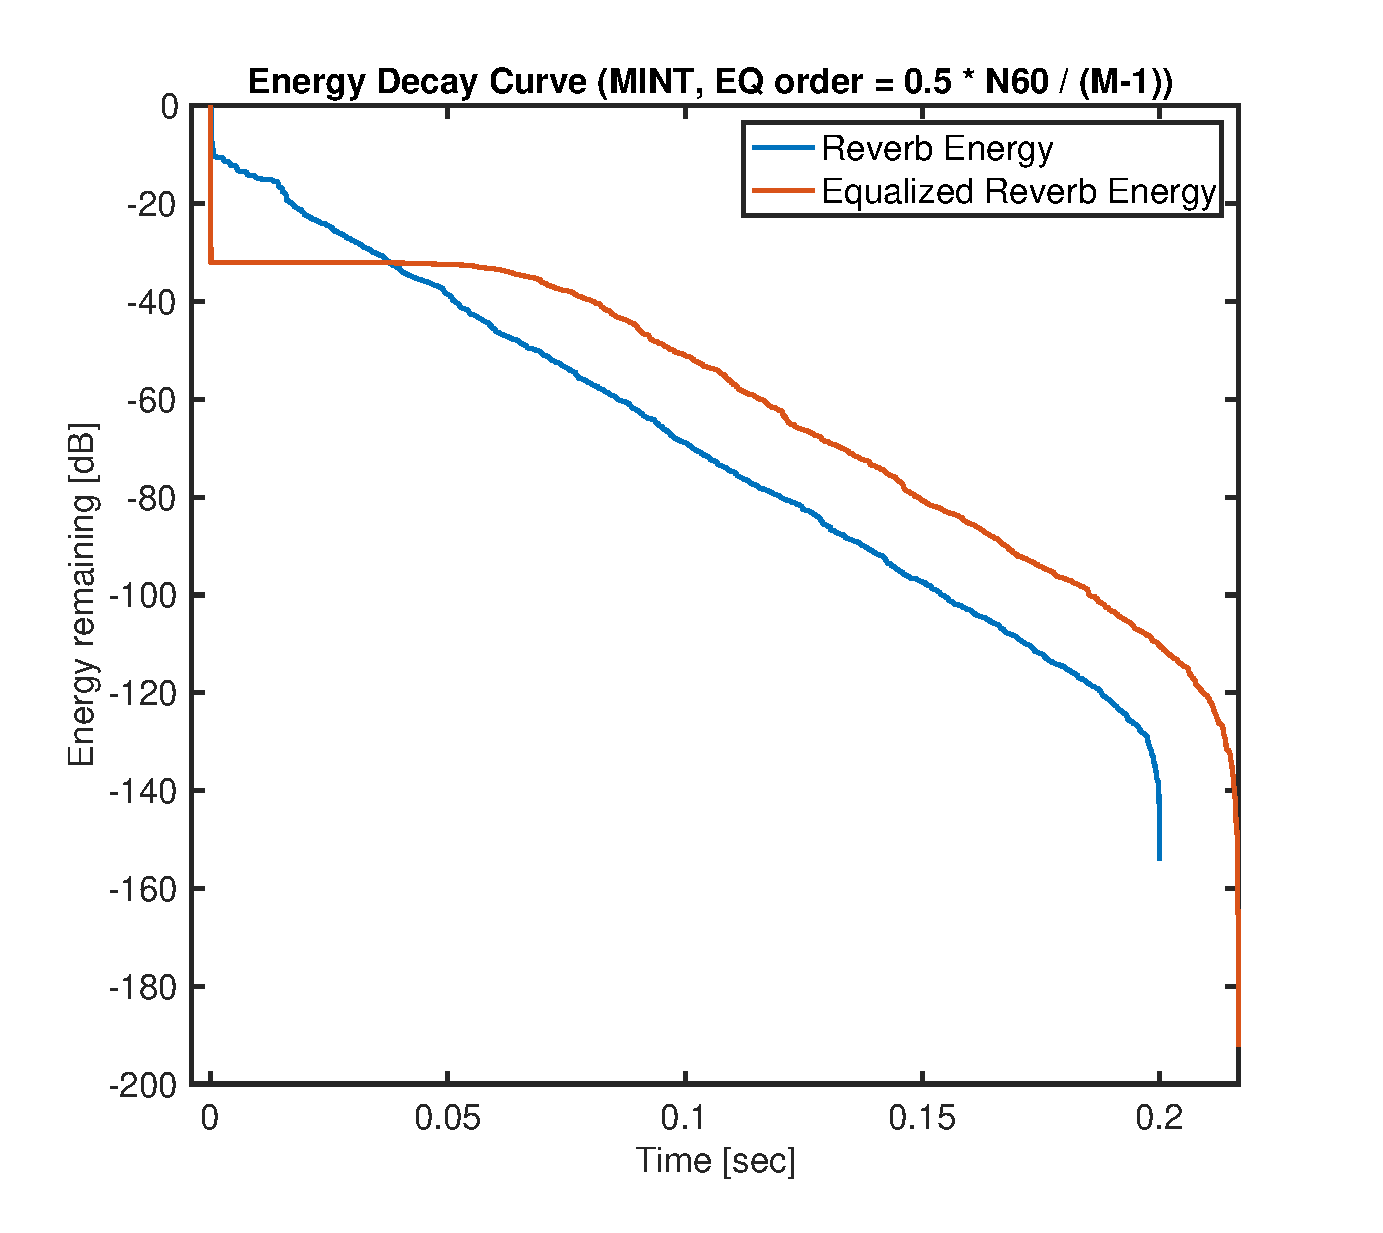
\includegraphics[width=\linewidth]{MINT_EDC_0p5N60_div_M_minus_1}
			\end{subfigure}
		\end{minipage}
	}
	% Dummy subfigure for referencing row D
	\refstepcounter{subfigure}
	\label{subfig:params_p2_MINT_compare:D}
	
		\caption{MINT equalizer performance for various equalizer orders relative to the actual length of the FIR channel ($L$) and the number of samples corresponding to the T60 of the channel ($\mathrm{N60} = \mathrm{T60}  \cdot \mathrm{sample\ rate}$)}
	\label{fig:params_p2_MINT_compare}
	
\end{figure}

\subsection{Multichannel Linear Prediction Inverse Filtering Results} \label{section:params_p2_MC_LP} 

To analyze the behavior of the multichannel linear prediction stage in isolation, without the performance impact of blindly estimating the AR properties of the source signal, the source-whitening stage was trained on the clean speech signal (i.e., supervised estimation of AR properties). One might suggest instead using a white noise sequence as the source signal and bypassing the source whitening stage altogether, but it was found that due to the high frequency resolution of the high-order multichannel linear prediction stage, the ripples in the specific realization of the uncorrelated random process would be whitened thus distorting the estimate of the true multichannel RTF inverse. Several multichannel prediction orders ($p_2$) were evaluated, covering the same equalizer filter lengths as in Figure \ref{fig:params_p2_MINT_compare}. A source-whitening prediction order of $p_1 = 4000$ was used accross all cases. The sample rate was \qty{16}{\kilo\hertz}, the source signal was a male talker ("SA1",  \textbf{TBD which collection/talker, couldn't find it when I looked} ) taken from the TMIT speech sample database \citep{garofolo1993timit} and synthetically looped to \qty{21.8}{\sec}, and the RIR was the same 4-channel \qty{100}{\milli\sec}-T60 RIR used in the previous section. The individual RIRs were manually time aligned, and the non-zero measurement noise samples leading the direct sound were manually set to zero. If leading measurement noise were not removed from the RIRs, these noise samples would be convolved with the source signal in sumulation as though they were real reflections that lead the direct sound. The MC-LP stage will always equalize to the first non-zero impulse because later impulses will be predictable from previous ones and therefore will be cancelled. Leaving the leading measurement noise samples would have an unrealistic negative impact on dereverberation performance since these samples are small relative to the actual RIR and thus also small relative to the residual reverberation left un-cancelled by the algorithm.

The source-whitening stage is shown in Figure \ref{fig:params_p2_stage1}, and the resulting EIRs and EDCs of all cases are shown in Figure \ref{fig:params_p2_compare}. The source-whitening result shows the estimated source spectrum (i.e., the LPC inverse filter) compared to the true power spectrum of the clean source signal in the first pane. The second pane shows resulting whitened power spectrum of the clean source signal, which was generated by applying the source-whitening filter to the clean signal instead of the reverberant signals.  For more detailed plots of the inner-workings of the algorithm in this evaluation, refer to Appendix \ref{section:appendix:params_p2}. 

% Test Conditions for all:
% - Source Signal = SA1.WAV
% - Source length = 348366
% - RIR = MYRiAD SAL Measured RIR (T60 = 2100 msec, Truncated Exponentially to T60 = 100 msec)
% - RIR length = 3200
% - T60 = 100 msec (N60 = 1600 samples)
% - SNR = 300 dB
% - Noise Signal = office ventilation
% - SIR = Inf dB
% - Interference Signal = None
%
% Delay-and-Predict config:
% - Number of Microphones (M) = 4
% - Source whitening order (p1) = 4000
% - Multichannel Linear Prediction order (p2) = varied
% - Source whitening Enabled? = 1
% - Source whitening on clean speech? = 1


\begin{figure}[H]
	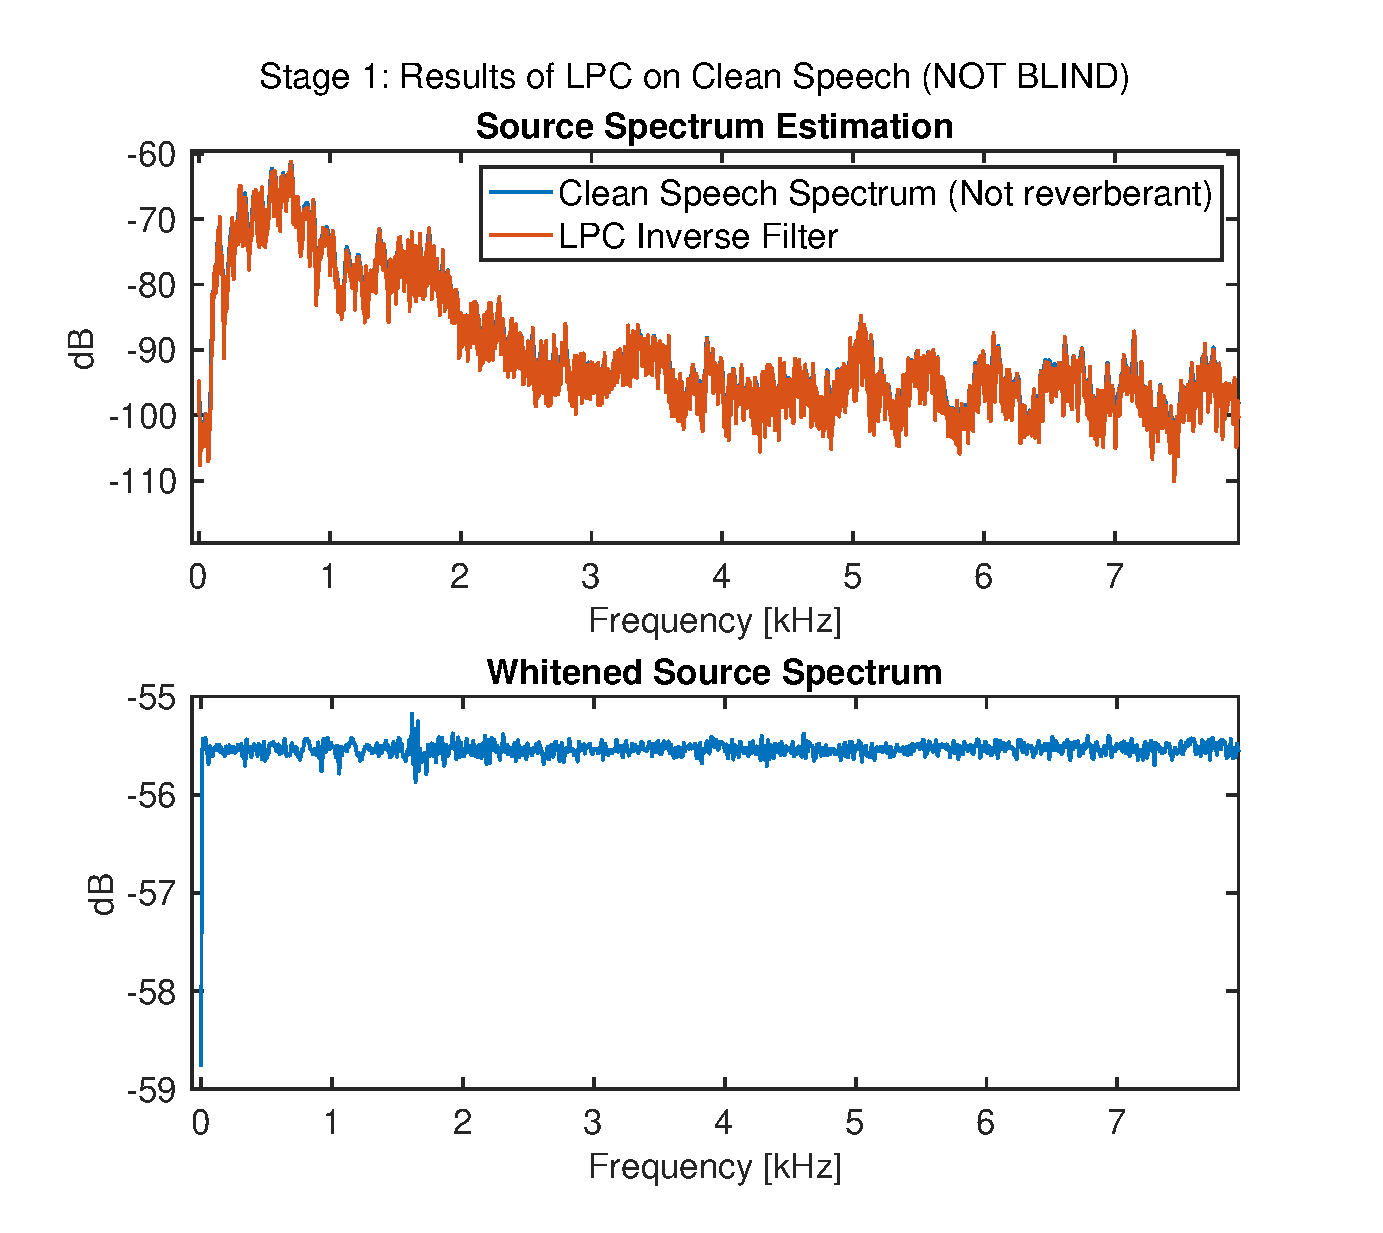
\includegraphics[width=0.49\textwidth]{S1_N60_div_M_minus_1}
	\centering
	\caption{Source whitening results using a $\mathrm{p1} = 4000$ order linear predictor. The prediction error filter coefficients were computed based on clean speech and the same filter was used in all tests in this section to assess the multichannel prediction stage of the delay-and-predict algorithm in isolation.}
	\label{fig:params_p2_stage1}
\end{figure}


\begin{figure}[H]
	\centering
	
	% ROW A
	\makebox[\textwidth][l]{%
		\begin{minipage}{0.23\textwidth}
			\centering
			\raggedleft{\footnotesize \textbf{(a)} \newline $p_2 = L / (M-1)$} \\
		\end{minipage}%
		\begin{minipage}{0.66\textwidth}
			\begin{subfigure}[t]{0.49\textwidth}
				\centering
				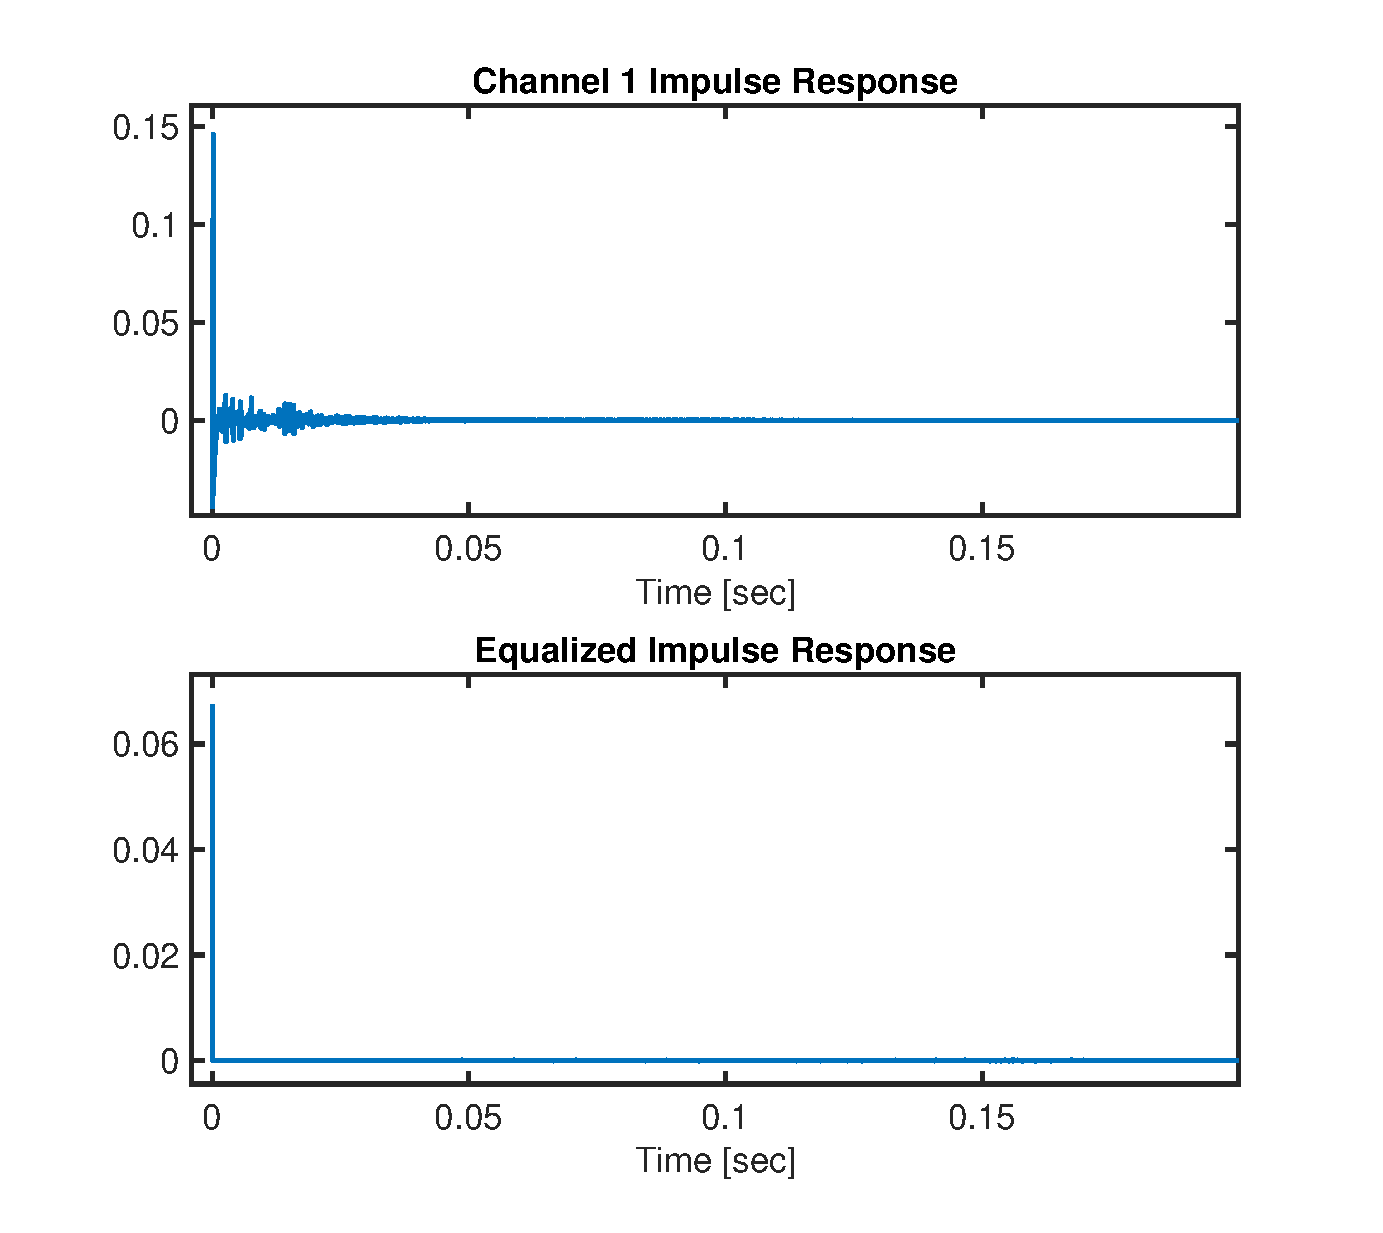
\includegraphics[width=\linewidth]{EIR_L_div_M_minus_1}
			\end{subfigure}
			\hfill
			\begin{subfigure}[t]{0.49\textwidth}
				\centering
				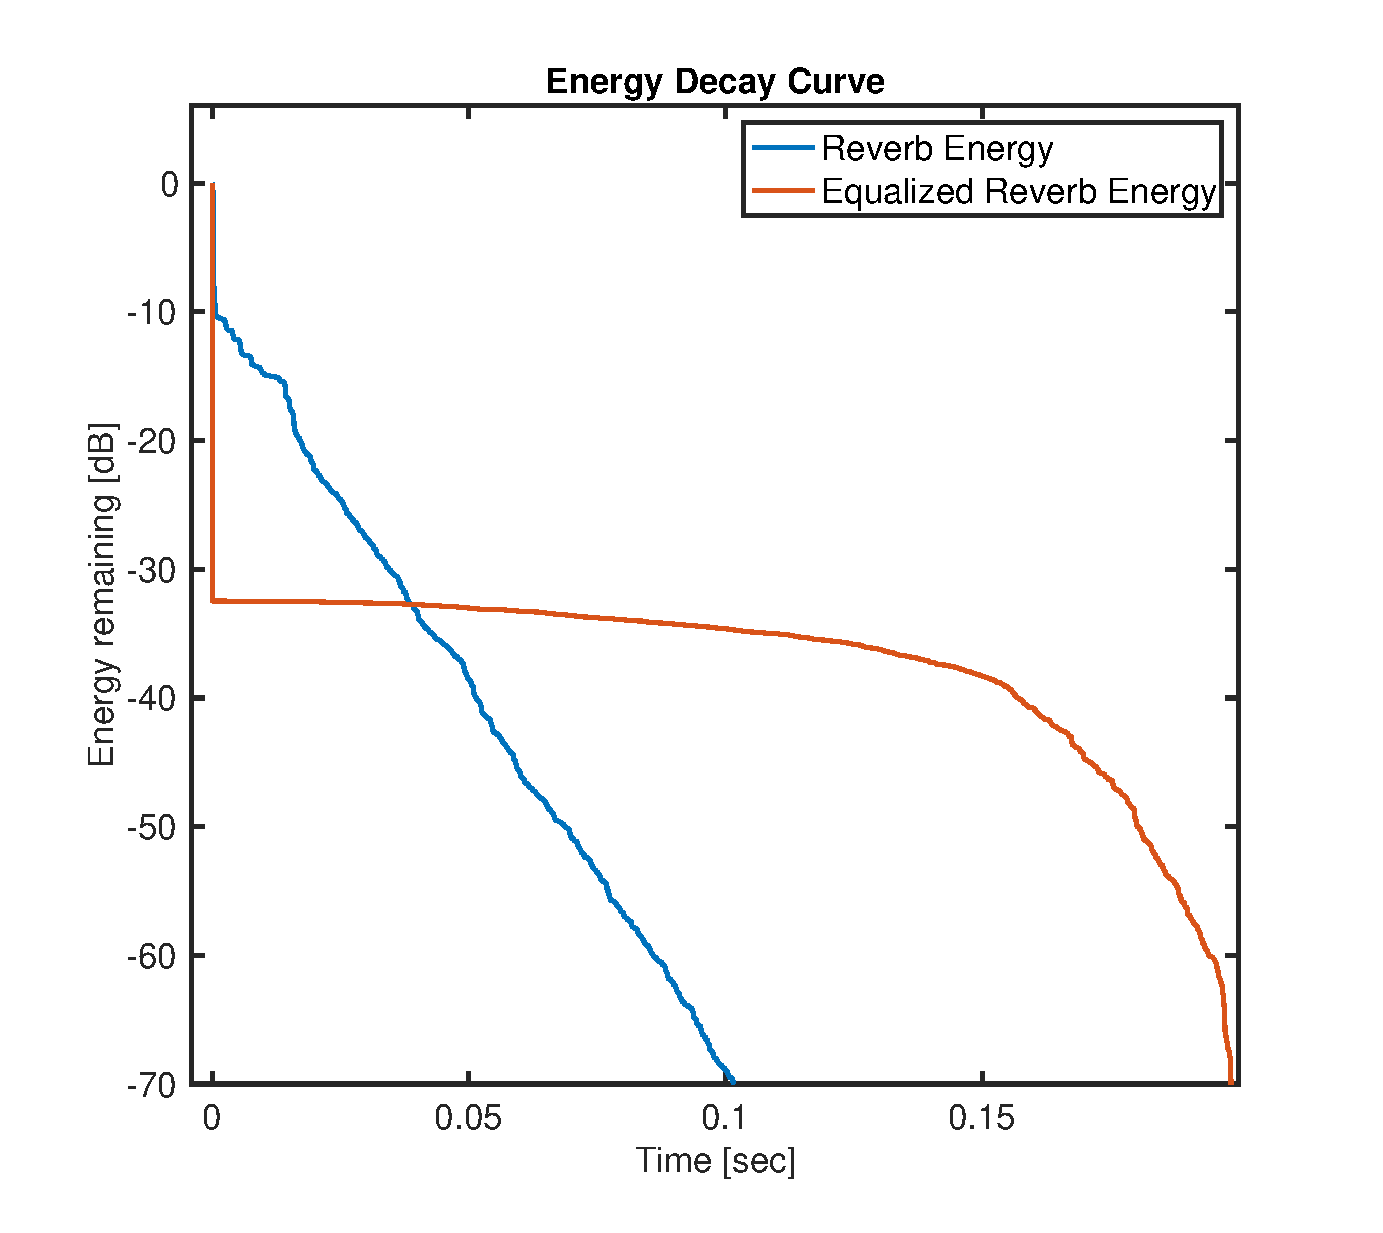
\includegraphics[width=\linewidth]{EDC_L_div_M_minus_1}
			\end{subfigure}
		\end{minipage}
	}
	% Dummy subfigure for referencing row A
	\refstepcounter{subfigure}
	\label{subfig:params_p2_compare:A}
	
	\vspace{1em}
	
	% ROW B
	\makebox[\textwidth][l]{%
		\begin{minipage}{0.23\textwidth}
			\centering
			\raggedleft{\footnotesize \textbf{(b)} \newline $p_2 = \mathrm{N60}  / (M-1)$} \\
		\end{minipage}%
		\begin{minipage}{0.66\textwidth}
			\begin{subfigure}[t]{0.49\textwidth}
				\centering
				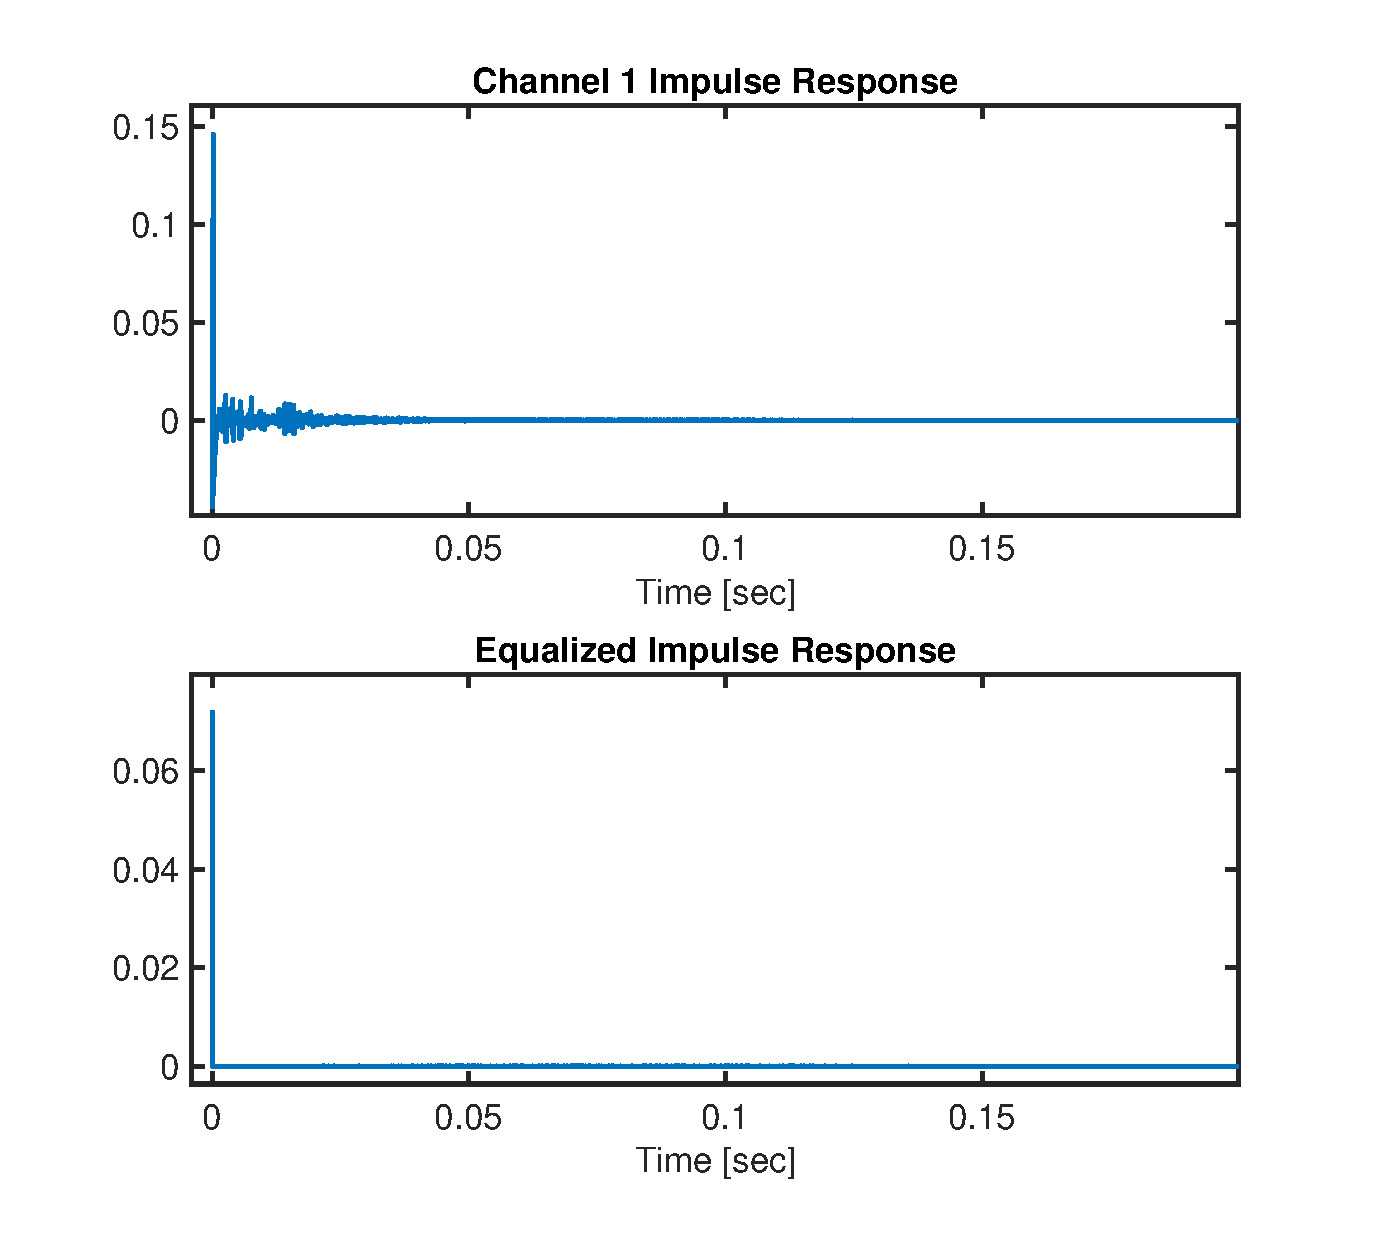
\includegraphics[width=\linewidth]{EIR_N60_div_M_minus_1}
			\end{subfigure}
			\hfill
			\begin{subfigure}[t]{0.49\textwidth}
				\centering
				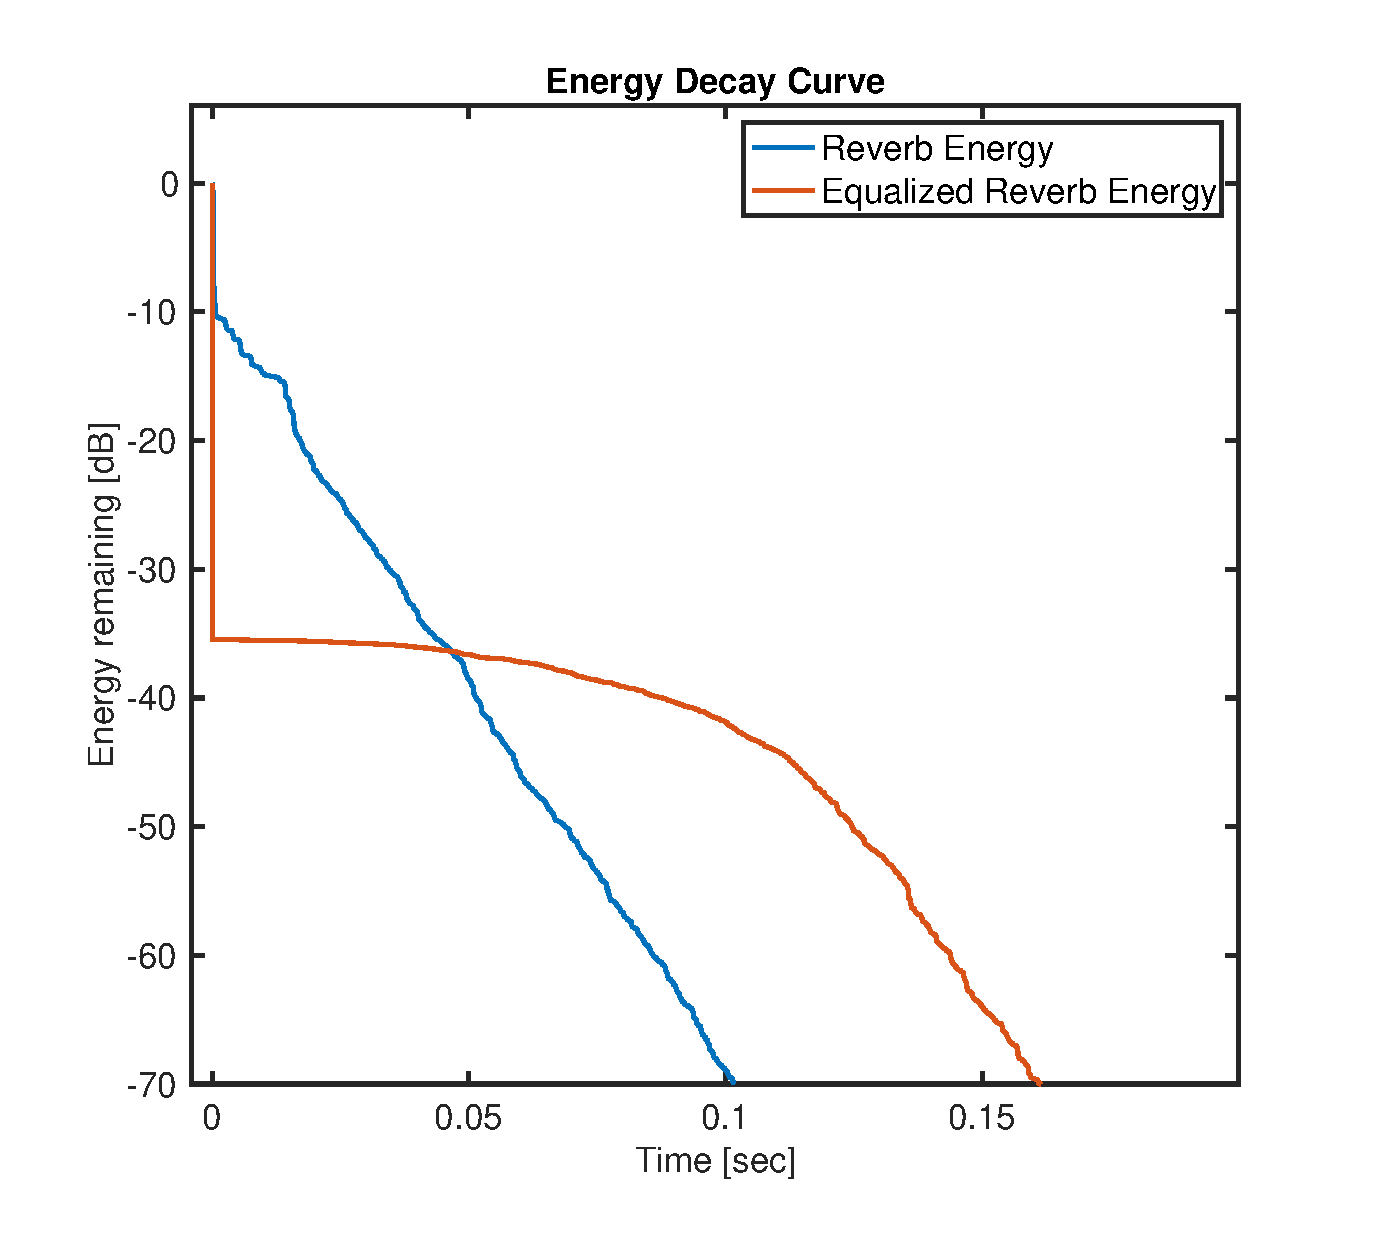
\includegraphics[width=\linewidth]{EDC_N60_div_M_minus_1}
			\end{subfigure}
		\end{minipage}
	}
	% Dummy subfigure for referencing row B
	\refstepcounter{subfigure}
	\label{subfig:params_p2_compare:B}
	
	\vspace{1em}
	
	% ROW C
	\makebox[\textwidth][l]{%
		\begin{minipage}{0.23\textwidth}
			\centering
			\raggedleft{\footnotesize \textbf{(c)} \newline $p_2 = 0.75 \cdot \mathrm{N60}  / (M-1)$} \\
		\end{minipage}%
		\begin{minipage}{0.66\textwidth}
			\begin{subfigure}[t]{0.49\textwidth}
				\centering
				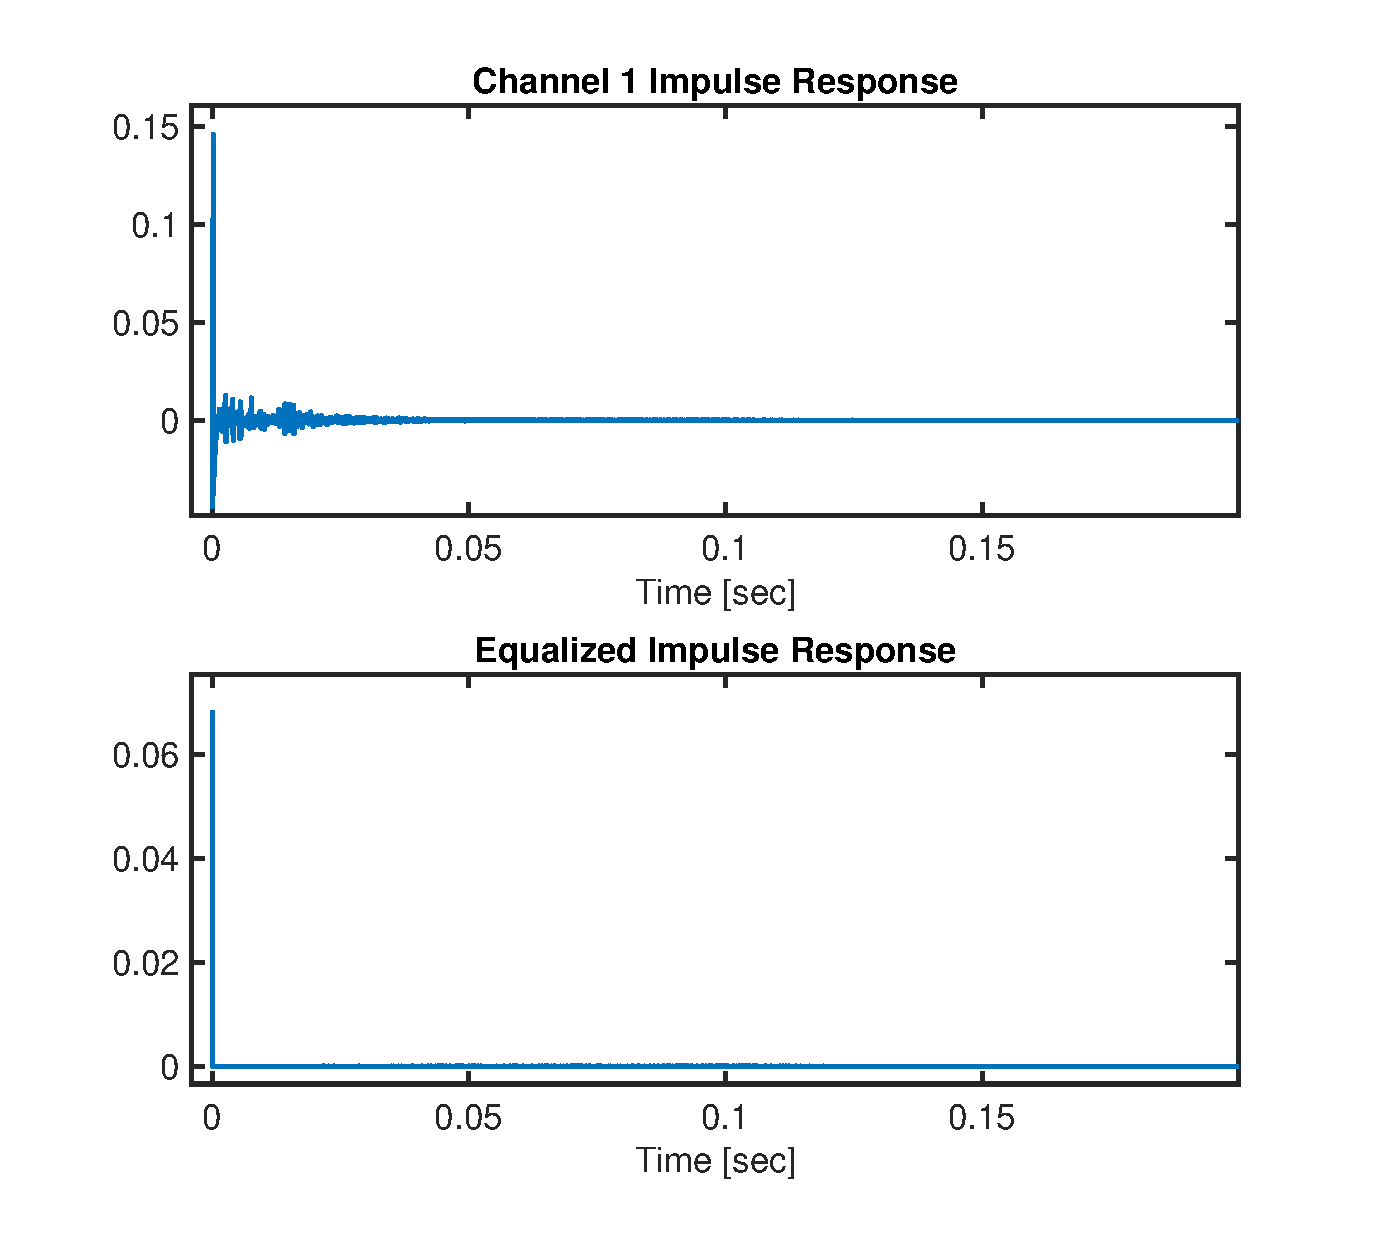
\includegraphics[width=\linewidth]{EIR_0p75N60_div_M_minus_1}
			\end{subfigure}
			\hfill
			\begin{subfigure}[t]{0.49\textwidth}
				\centering
				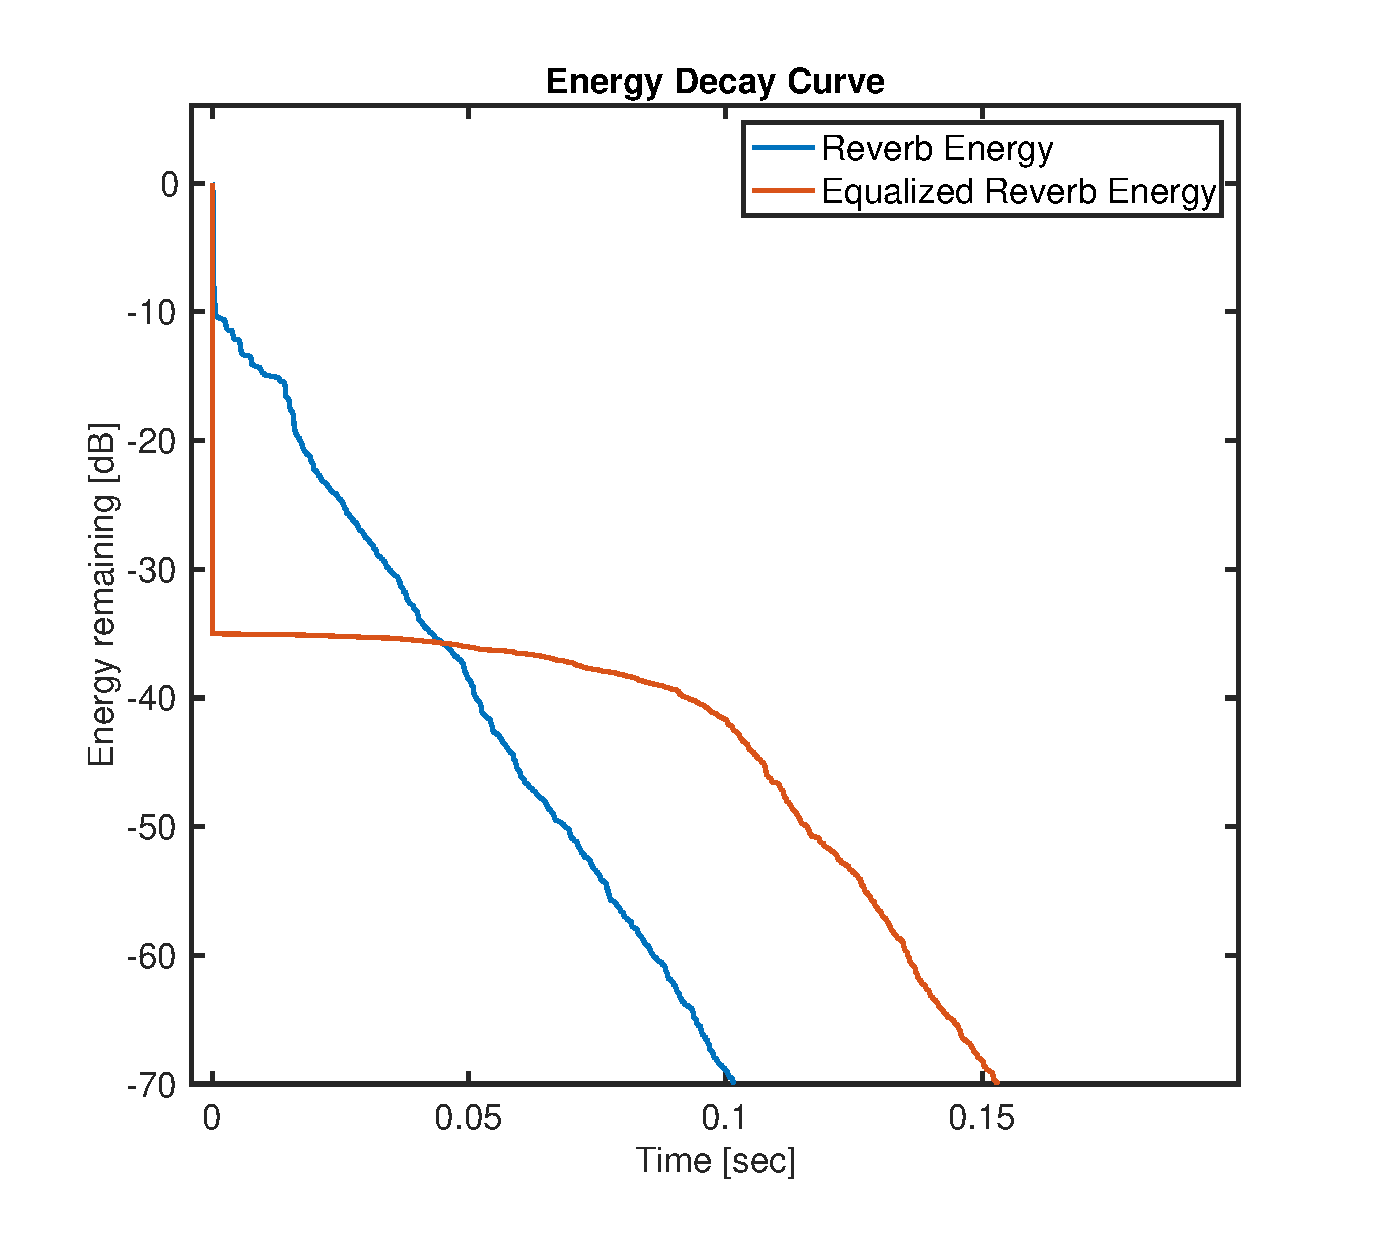
\includegraphics[width=\linewidth]{EDC_0p75N60_div_M_minus_1}
			\end{subfigure}
		\end{minipage}
	}
	% Dummy subfigure for referencing row C
	\refstepcounter{subfigure}
	\label{subfig:params_p2_compare:C}
	
	\vspace{1em}
	
	% ROW D
	\makebox[\textwidth][l]{%
		\begin{minipage}{0.23\textwidth}
			\centering
			\raggedleft{\footnotesize \textbf{(d)} \newline $p_2 = 0.5 \cdot \mathrm{N60}  / (M-1)$} \\
		\end{minipage}%
		\begin{minipage}{0.66\textwidth}
			\begin{subfigure}[t]{0.49\textwidth}
				\centering
				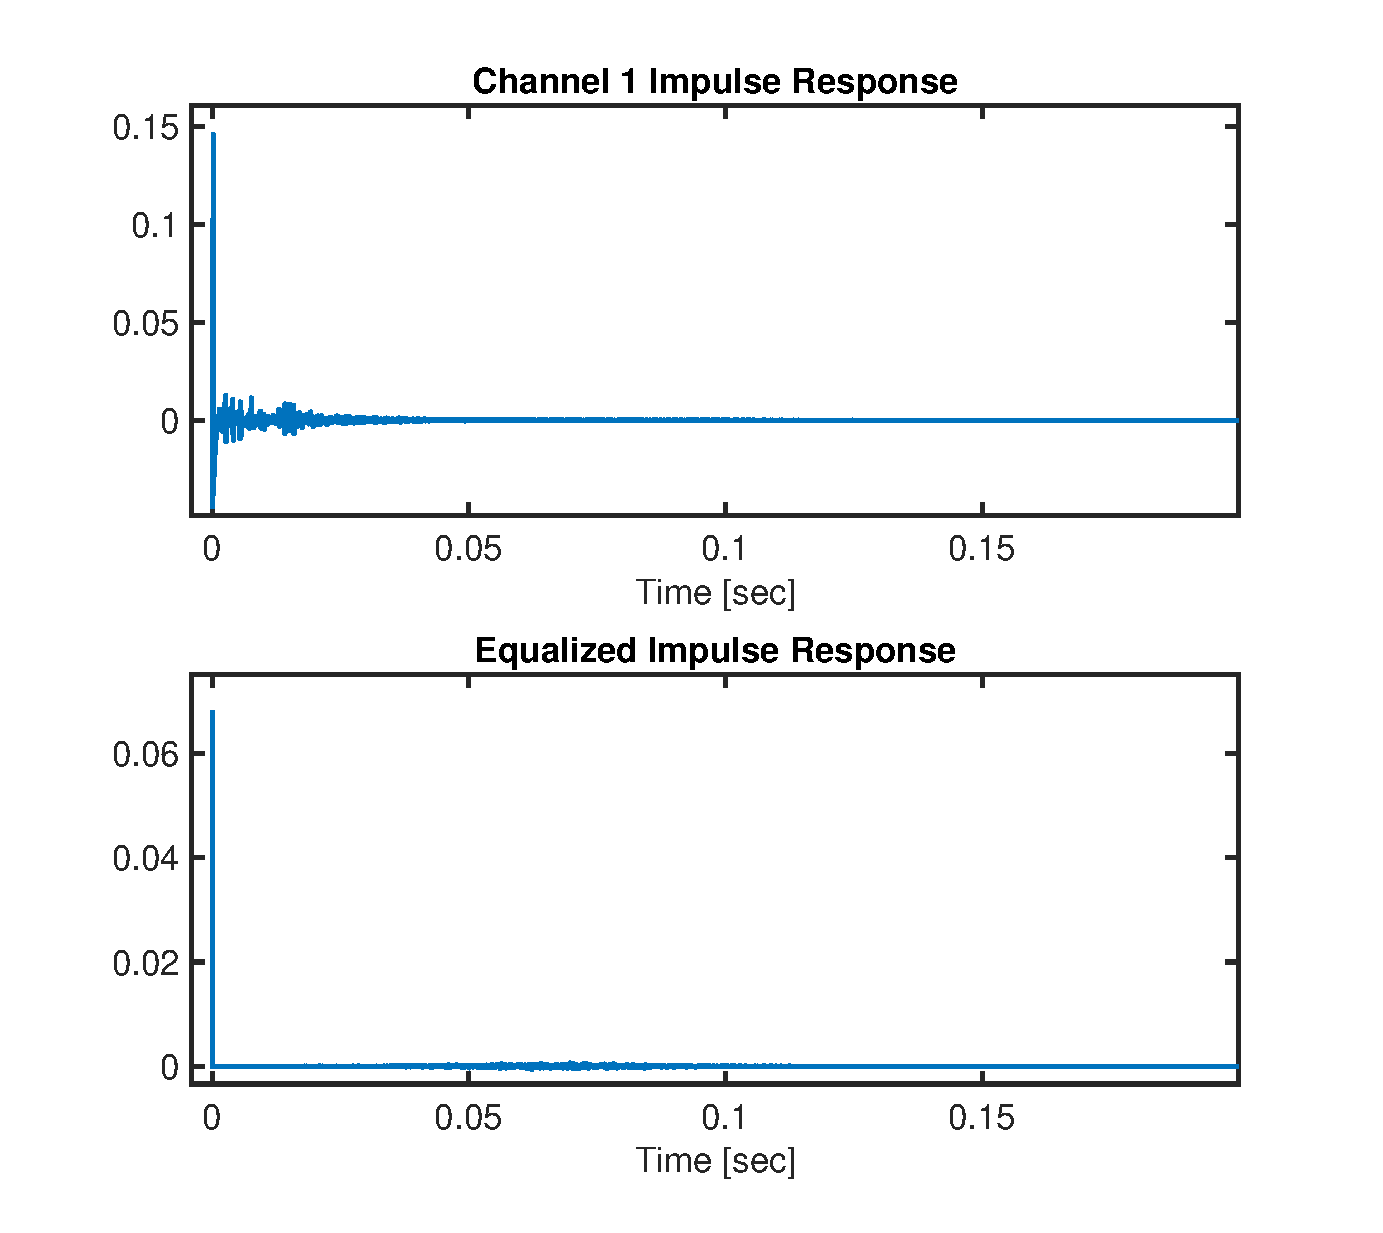
\includegraphics[width=\linewidth]{EIR_0p5N60_div_M_minus_1}
			\end{subfigure}
			\hfill
			\begin{subfigure}[t]{0.49\textwidth}
				\centering
				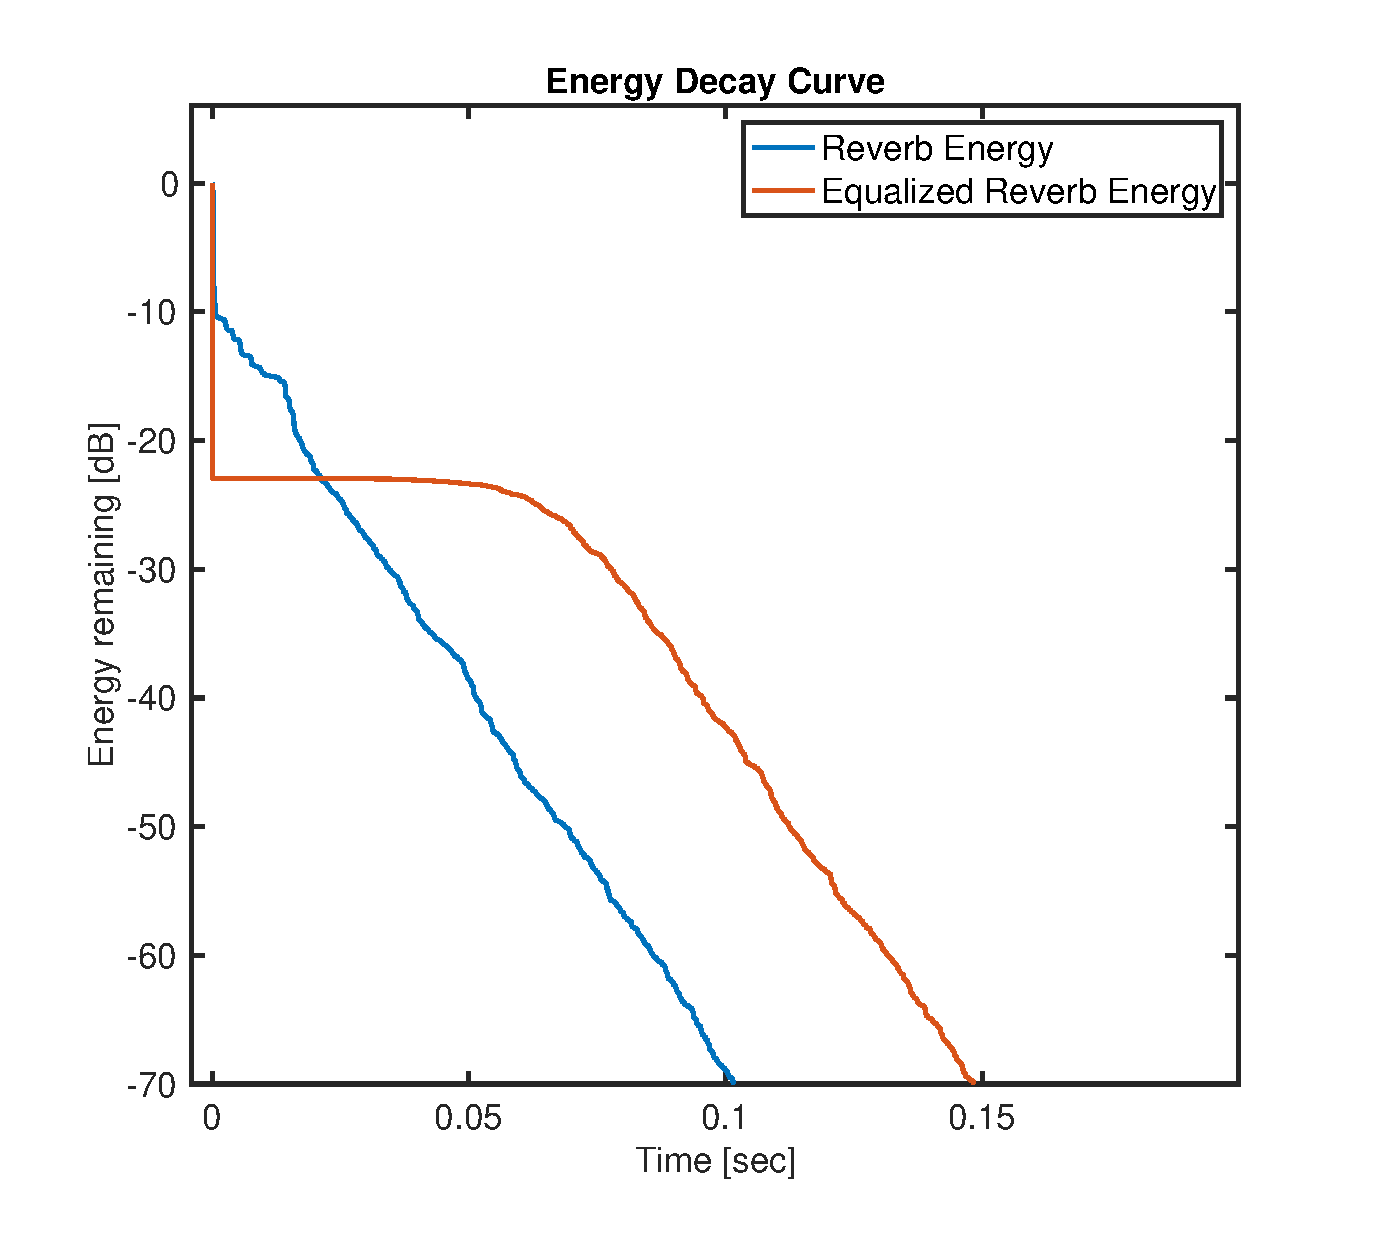
\includegraphics[width=\linewidth]{EDC_0p5N60_div_M_minus_1}
			\end{subfigure}
		\end{minipage}
	}
	% Dummy subfigure for referencing row D
	\refstepcounter{subfigure}
	\label{subfig:params_p2_compare:D}
	
	\caption{Delay-and-Predict dereverberation performance with various multichannel linear prediction orders ($\mathrm{p2}$) relative to the actual length of the FIR channel ($L$) and the number of samples corresponding to the T60 of the channel ($\mathrm{N60}$). Figure \ref{fig:params_p2_stage1} shows the common source whitening filter used.}
\label{fig:params_p2_compare}
	
\end{figure}

Accross all test cases, it was noted that reverberation cancellation performance of the inverse filter produced by multichannel linear prediction was significantly worse than the MINT inverse filter. While $p_2=L/\left(M-1\right)$ results in \qty{250}{\decibel} of reverberation cancellation in the MINT inverse filter, the MC-LP-estimated inverse filter only acheives approximately \qty{32}{\decibel} cancellation. This makes sense since the multichannel normal equations (Equation \ref{eq:mc_yule_walker}) are susceptable to numerical error which results in estimation variance. This is especially true for the weaker tail of the RIR, where reverberation energy is smaller (i.e., the effective SNR of the reverberation is lower) and estimation variance is larger. The higher estimation variance occurs due to the longer autocorrelation lags invovled in the normal equations, for which there is less data available (less overlapping data between the lagged and not-lagged signals). This practical effect of estimating correlation is well known and is the motivation for biased estimators such as the windowed autcorrelation estimator used in the periodogram PSD estimator.\citep{oppenheim1999discrete}. Additionally, although the source-whitening filter was trained on the clean speech signal, it has its own estimation variance and is performance is also limited by its finite prediction order ($p_1 = 4000$). Any imperfections in the source-whitening will distort the MC-LP results.

Interestingly, reverberation suppression was observed to effectively plateau at around \qty{30}{\decibel} - \qty{35}{\decibel} for $p_2 >= 0.75 \cdot \mathrm{N60} / \left(M-1\right)$. Essentially, the RIR is early perfectly equalized almost instantaneously (like the MINT), but towards the end of the reverberation tail, increased estimation variance leads to increasingly worse performance, resulting in reverberation energy increasing again. 

Therefore, it was concluded that it is not possible in practice to acheive the near-perfect cancellation dicated by the MINT when using MC-LP-based dereverberation algorithms. For this reason, it does not make sense to choose $p_2$ based on the MINT conditions for perfect equalization, but rather based on the practical boundaries resulting from numerical limitations. Figure \ref{fig:params_p2_compare} suggests that setting $p_2$ greater than approximately $0.75 \cdot \mathrm{N60} / \left(M-1)\right)$ is reasonable. In practice, the $N60$ is unknown, so the MC-LP prediction order should be set as high as is computationally acceptable to sufficiently cancel the longest T60s possible.

\section{Source Whitening Linear Prediction Order} \label{section:params_p1} 

To evaluate the impact of the source-whitening prediction order ($p_1$), the MC-LP order was fixed at $p_2 = \mathrm{N60} / \left(M-1\right)$, and $p_1$ was varied. The same sample rate, source signal/length, and 4-channel RIR from Section \ref{section:params_p2_MC_LP} were used. The source-whitening prediction order $p_1=200$ was included to match the original configuration of \cite{triki2006delay} (scaled by sample rate from \qty{8}{\kilo\hertz} to \qty{16}{\kilo\hertz}), and $p_1 = p_2 \cdot \left(M-1\right)$ was included to match the effective spectral resolution of the MC-LP stage. Since the MINT dictates that a length-$L$ RIR can be perfectly equalized using $M$ channels with $M$ corresponding length $\left(p_2+1\right) = \left(L-1\right)/\left(M-1\right)$ equalizer filters, it can be said that the effective spectral resolution of MINT equalizer (and therefore any multichannel equalizer) is that of a FIR filter of length $L= \left(p_2+1\right) \cdot \left(M-1\right)  + 1 \approx p_2 \cdot \left(M-1\right)$. Therefore setting $p_1 = p_2 \cdot (M-1)$ effectively matches the spectral resolution of the source-whitening stage to the MC-LP stage as previously stated. Figure \ref{fig:params_p1_compare} shows the EIR and EDC performance for each case. For more detailed plots of the inner-workings of the algorithm in this evaluation, refer to Appendix \ref{section:appendix:params_p1}.


% Test Conditions:
% - Source Signal = SA1.WAV
% - Source length = 348366
% - RIR = MYRiAD SAL Measured RIR (T60 = 2100 msec, Truncated Exponentially to T60 = 100 msec)
% - RIR length = 3200
% - T60 = 100 msec (N60 = 1600 samples)
% - SNR = 300 dB
% - Noise Signal = office ventilation
% - SIR = Inf dB
% - Interference Signal = None
%
% Delay-and-Predict config:
% - Number of Microphones (M) = 4
% - Source whitening order (p1) = varied
% - Multichannel Linear Prediction order (p2) = 533 (N60 / (M-1))
% - Source whitening Enabled? = 1
% - Source whitening on clean speech? = 1

\begin{figure}[H]
	\centering
	
	% ROW A
	\makebox[\textwidth][l]{%
		\begin{minipage}{0.23\textwidth}
			\centering
			\raggedleft{\footnotesize \textbf{(a)} \newline $p_1 = 200$ \newline \citep{triki2006delay}} \\
		\end{minipage}%
		\begin{minipage}{0.66\textwidth}
			\begin{subfigure}[t]{0.49\textwidth}
				\centering
				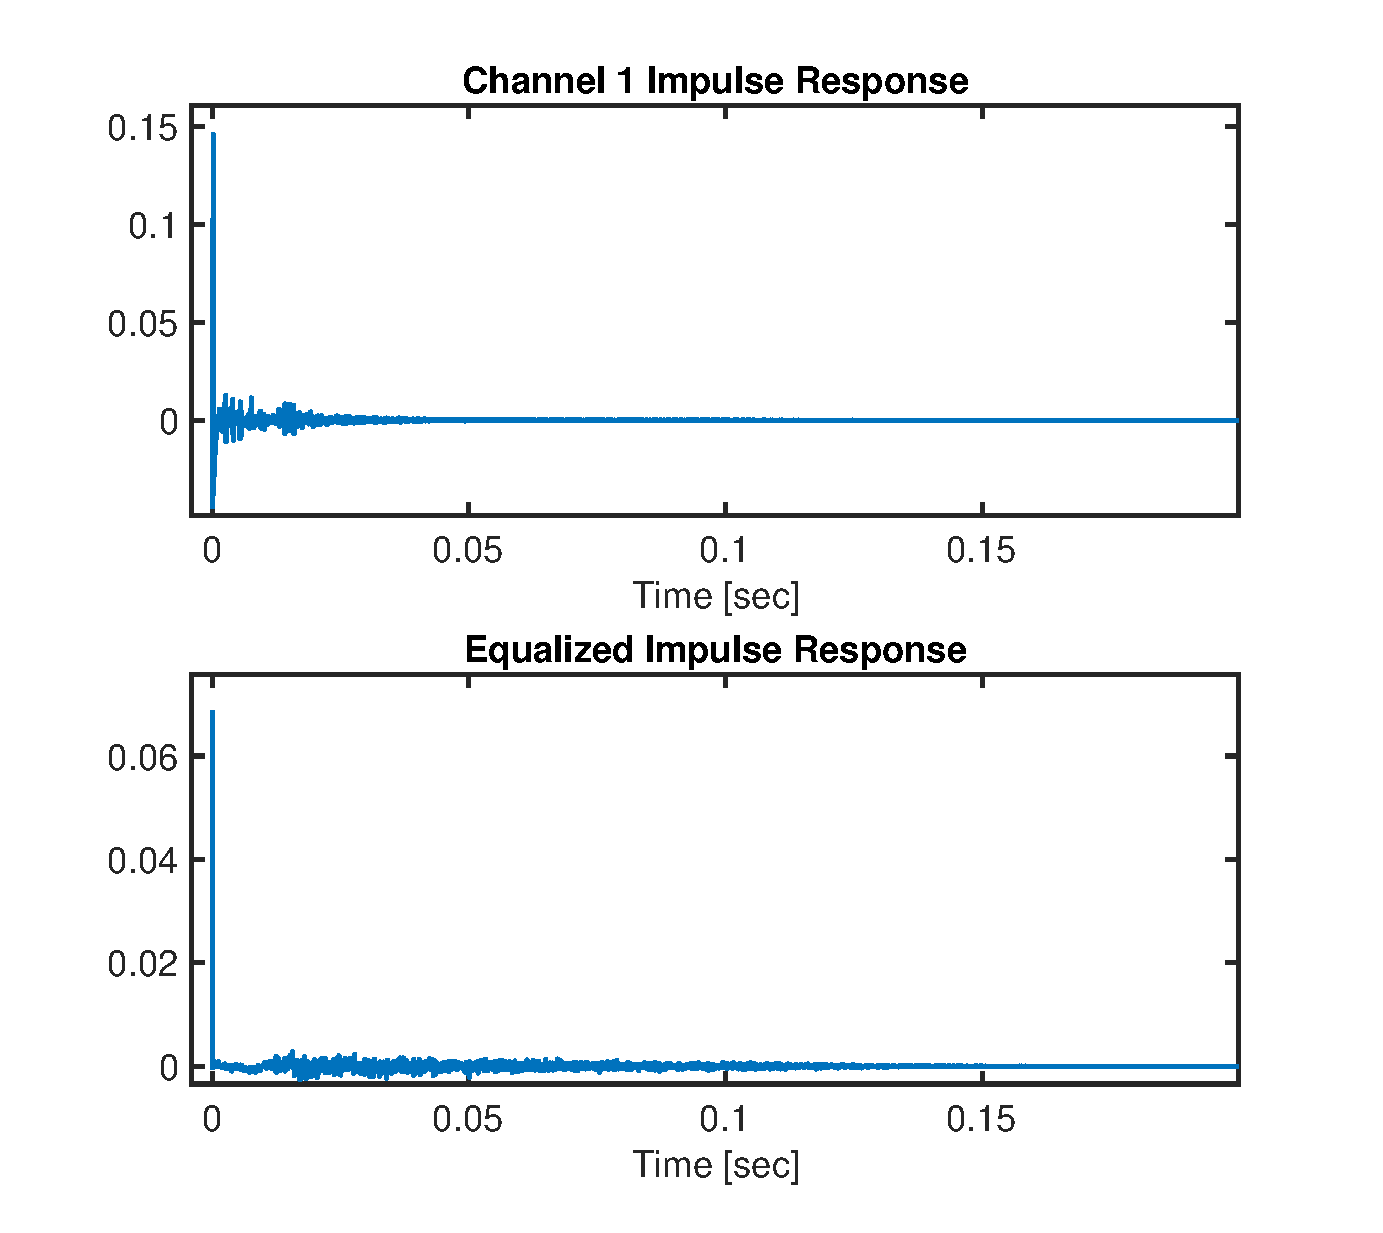
\includegraphics[width=\linewidth]{EIR_p1_200}
			\end{subfigure}
			\hfill
			\begin{subfigure}[t]{0.49\textwidth}
				\centering
				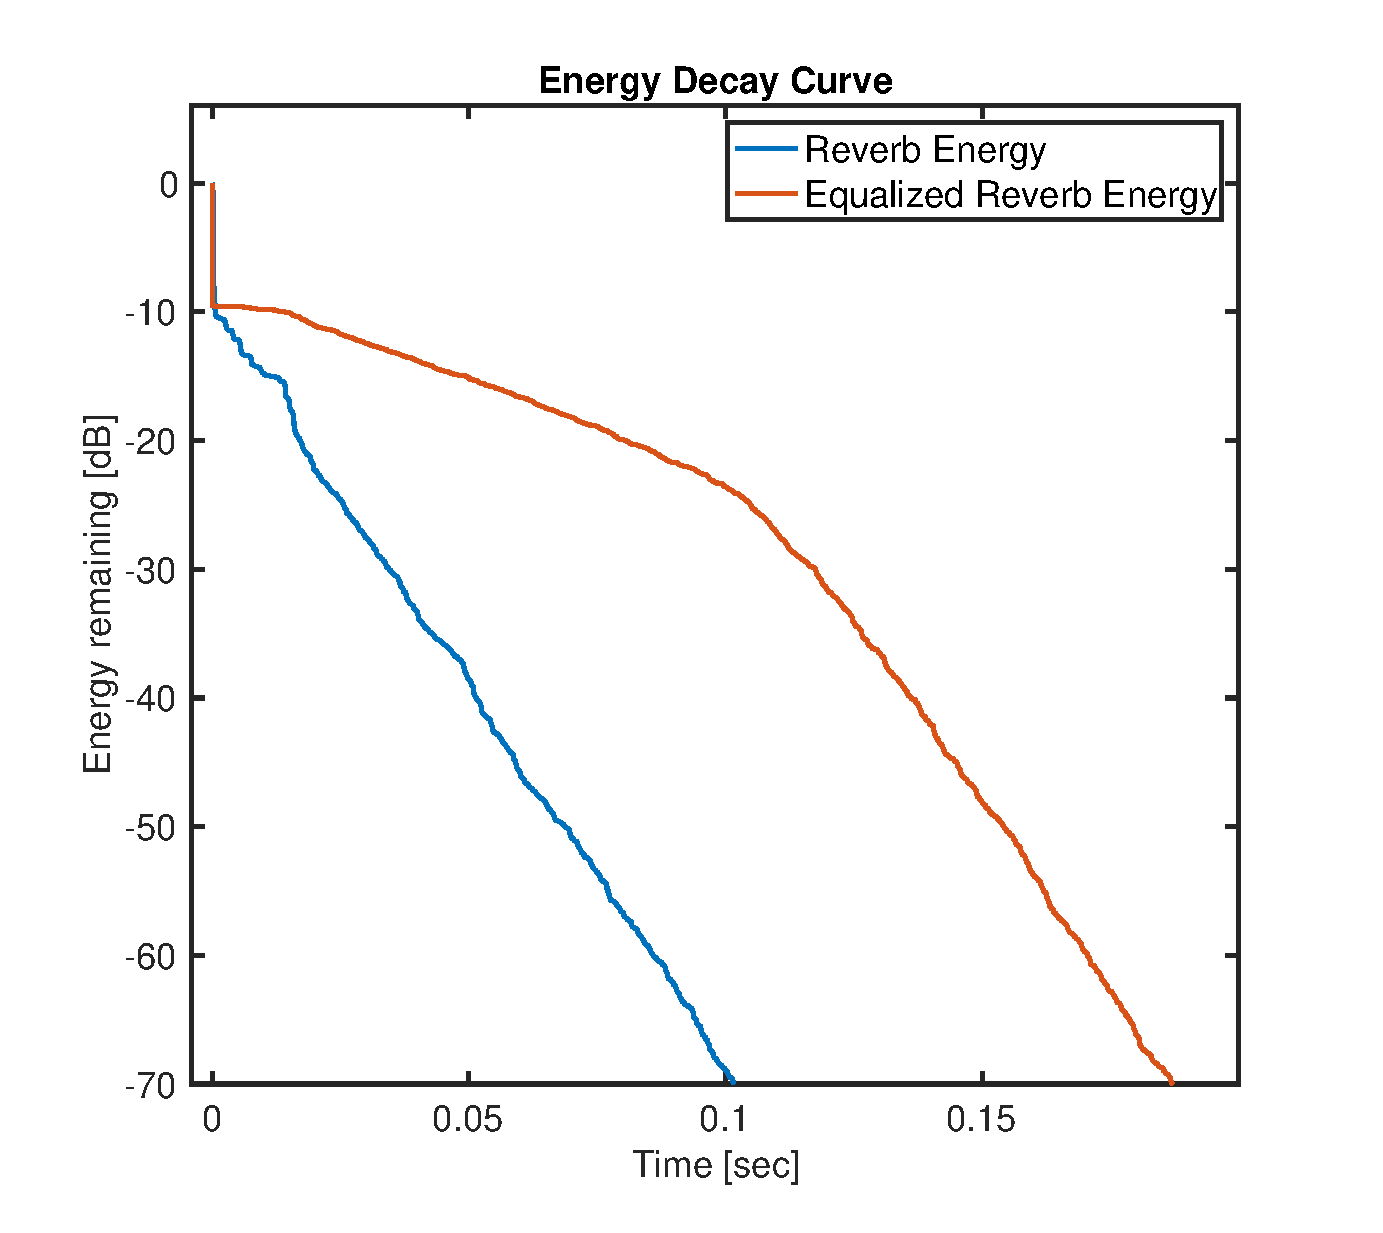
\includegraphics[width=\linewidth]{EDC_p1_200}
			\end{subfigure}
		\end{minipage}
	}
	% Dummy subfigure for referencing row A
	\refstepcounter{subfigure}
	\label{subfig:params_p1_compare:A}
	
	\vspace{1em}
	
	% ROW B
	\makebox[\textwidth][l]{%
		\begin{minipage}{0.23\textwidth}
			\centering
			\raggedleft{\footnotesize \textbf{(b)} \newline $p_1 = 1000$} \\
		\end{minipage}%
		\begin{minipage}{0.66\textwidth}
			\begin{subfigure}[t]{0.49\textwidth}
				\centering
				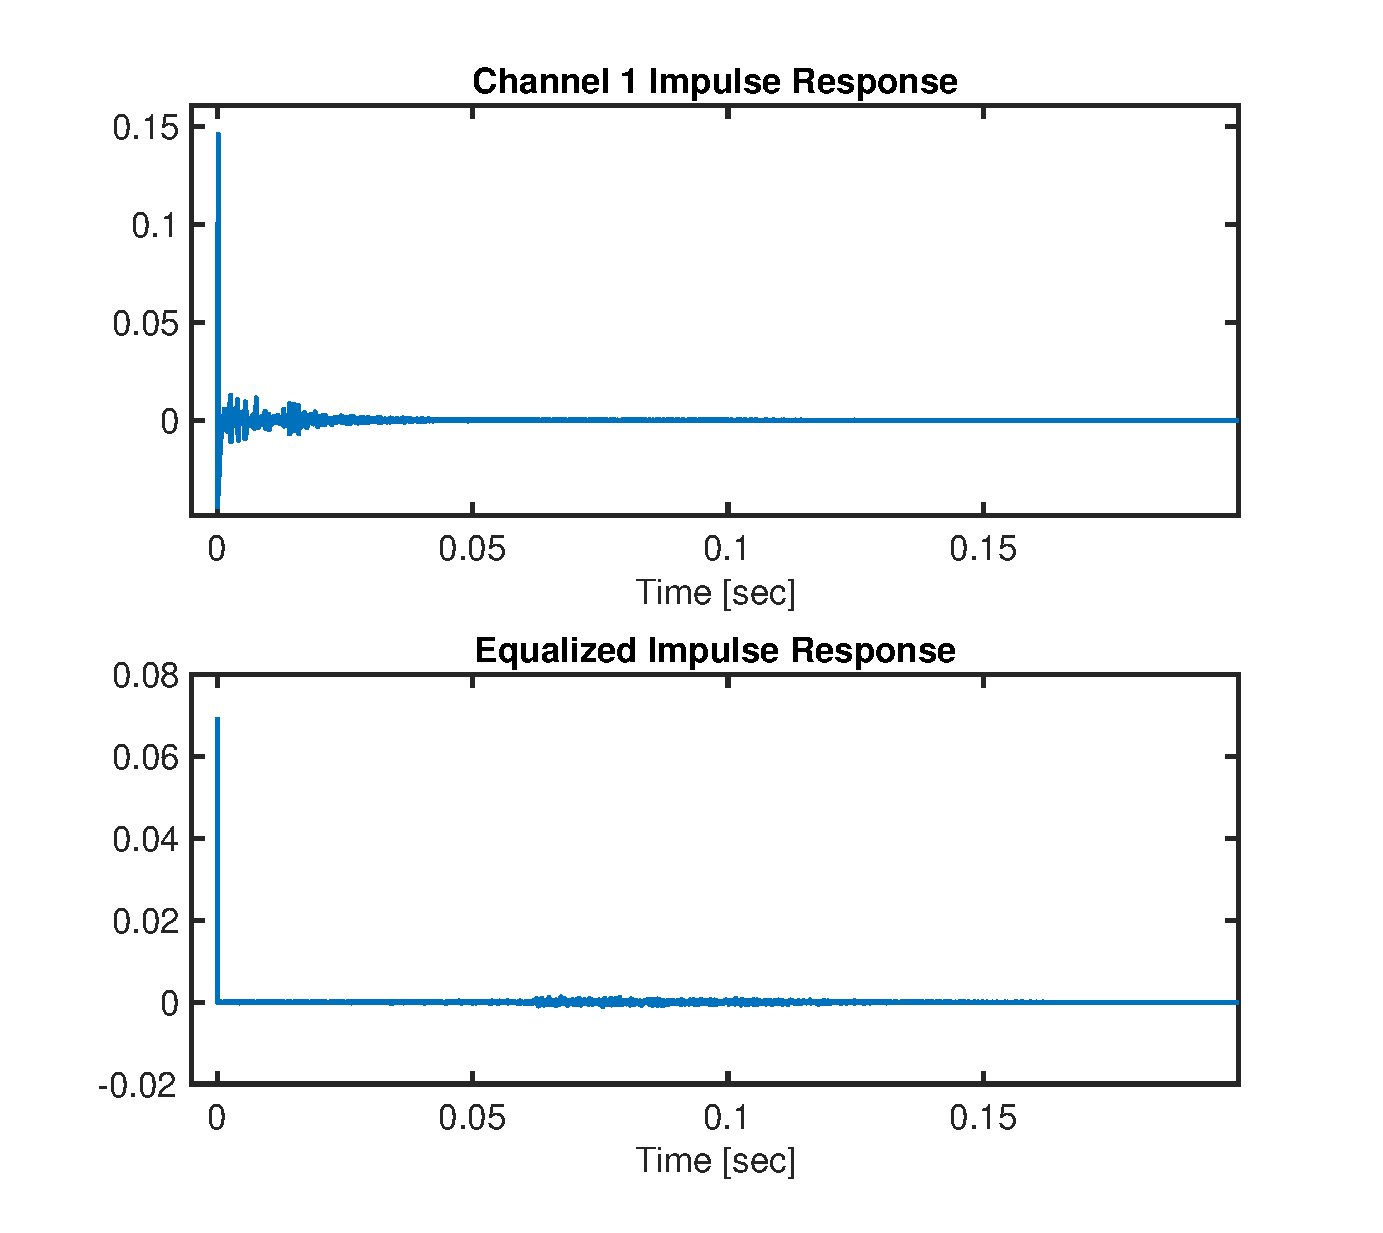
\includegraphics[width=\linewidth]{EIR_p1_1000}
			\end{subfigure}
			\hfill
			\begin{subfigure}[t]{0.49\textwidth}
				\centering
				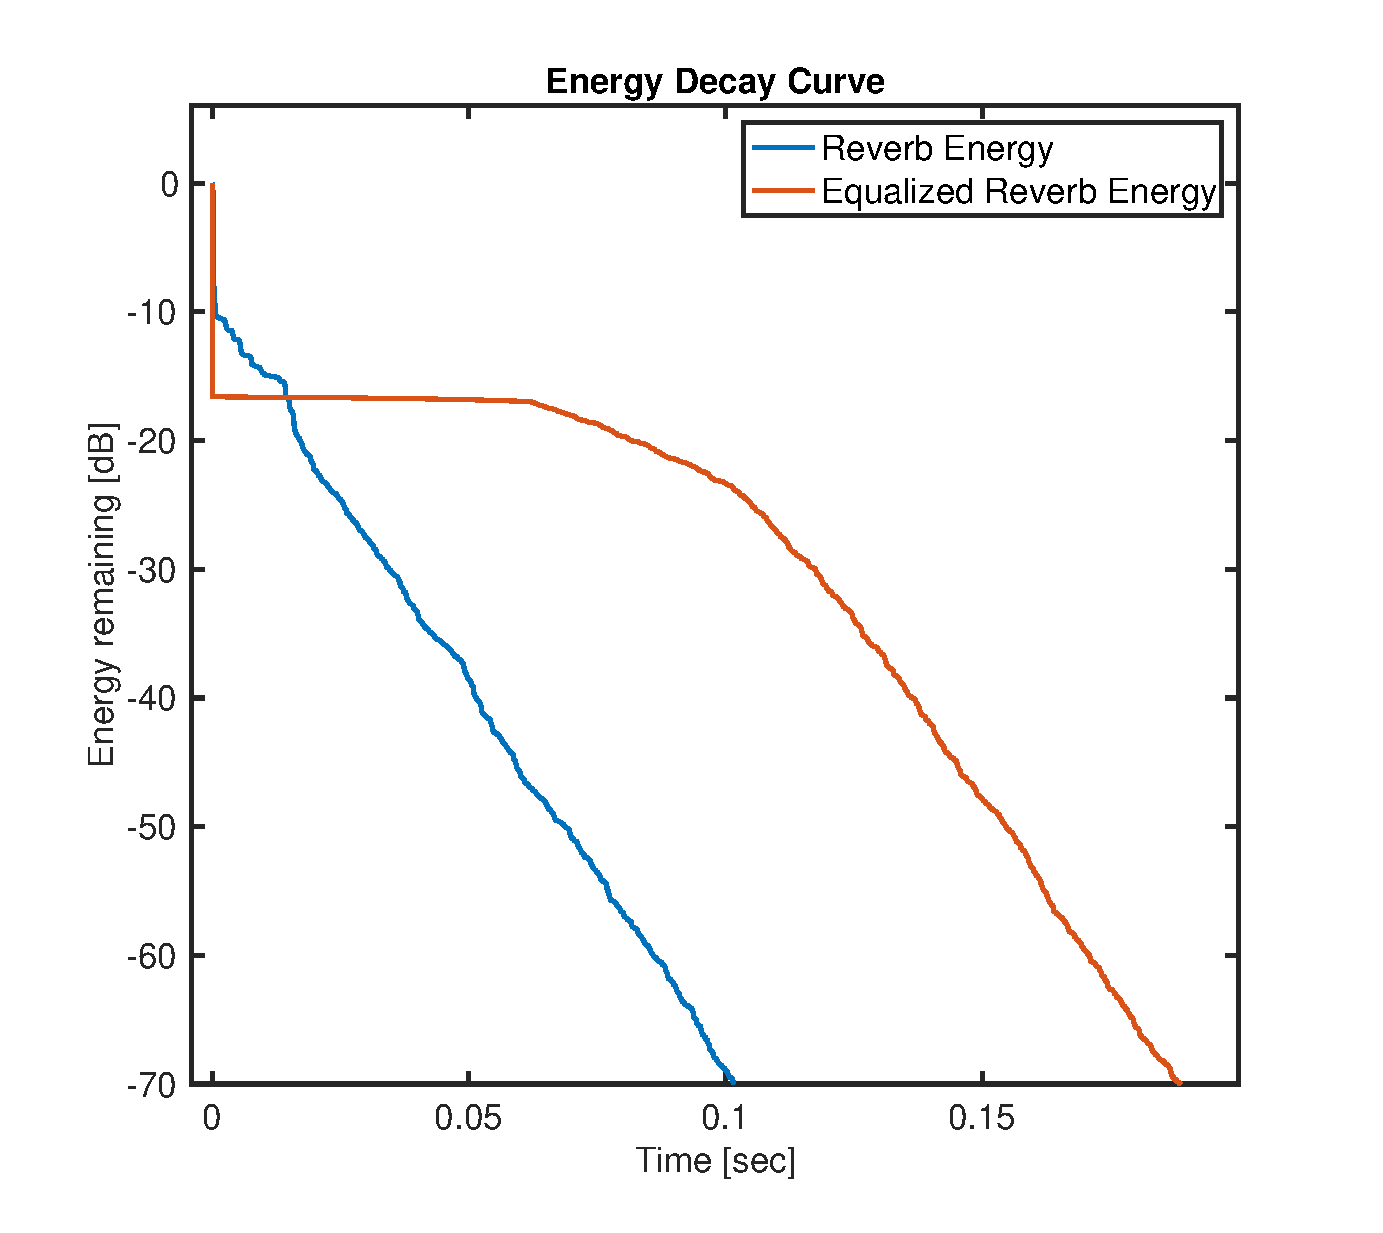
\includegraphics[width=\linewidth]{EDC_p1_1000}
			\end{subfigure}
		\end{minipage}
	}
	% Dummy subfigure for referencing row B
	\refstepcounter{subfigure}
	\label{subfig:params_p1_compare:B}
	
	\vspace{1em}
	
	% ROW C
	\makebox[\textwidth][l]{%
		\begin{minipage}{0.23\textwidth}
			\centering
			\raggedleft{\footnotesize \textbf{(c)} \newline $p_1 = 1600$ \newline ($p_1 = p2 \cdot \left(M-1\right)$)} \\
		\end{minipage}%
		\begin{minipage}{0.66\textwidth}
			\begin{subfigure}[t]{0.49\textwidth}
				\centering
				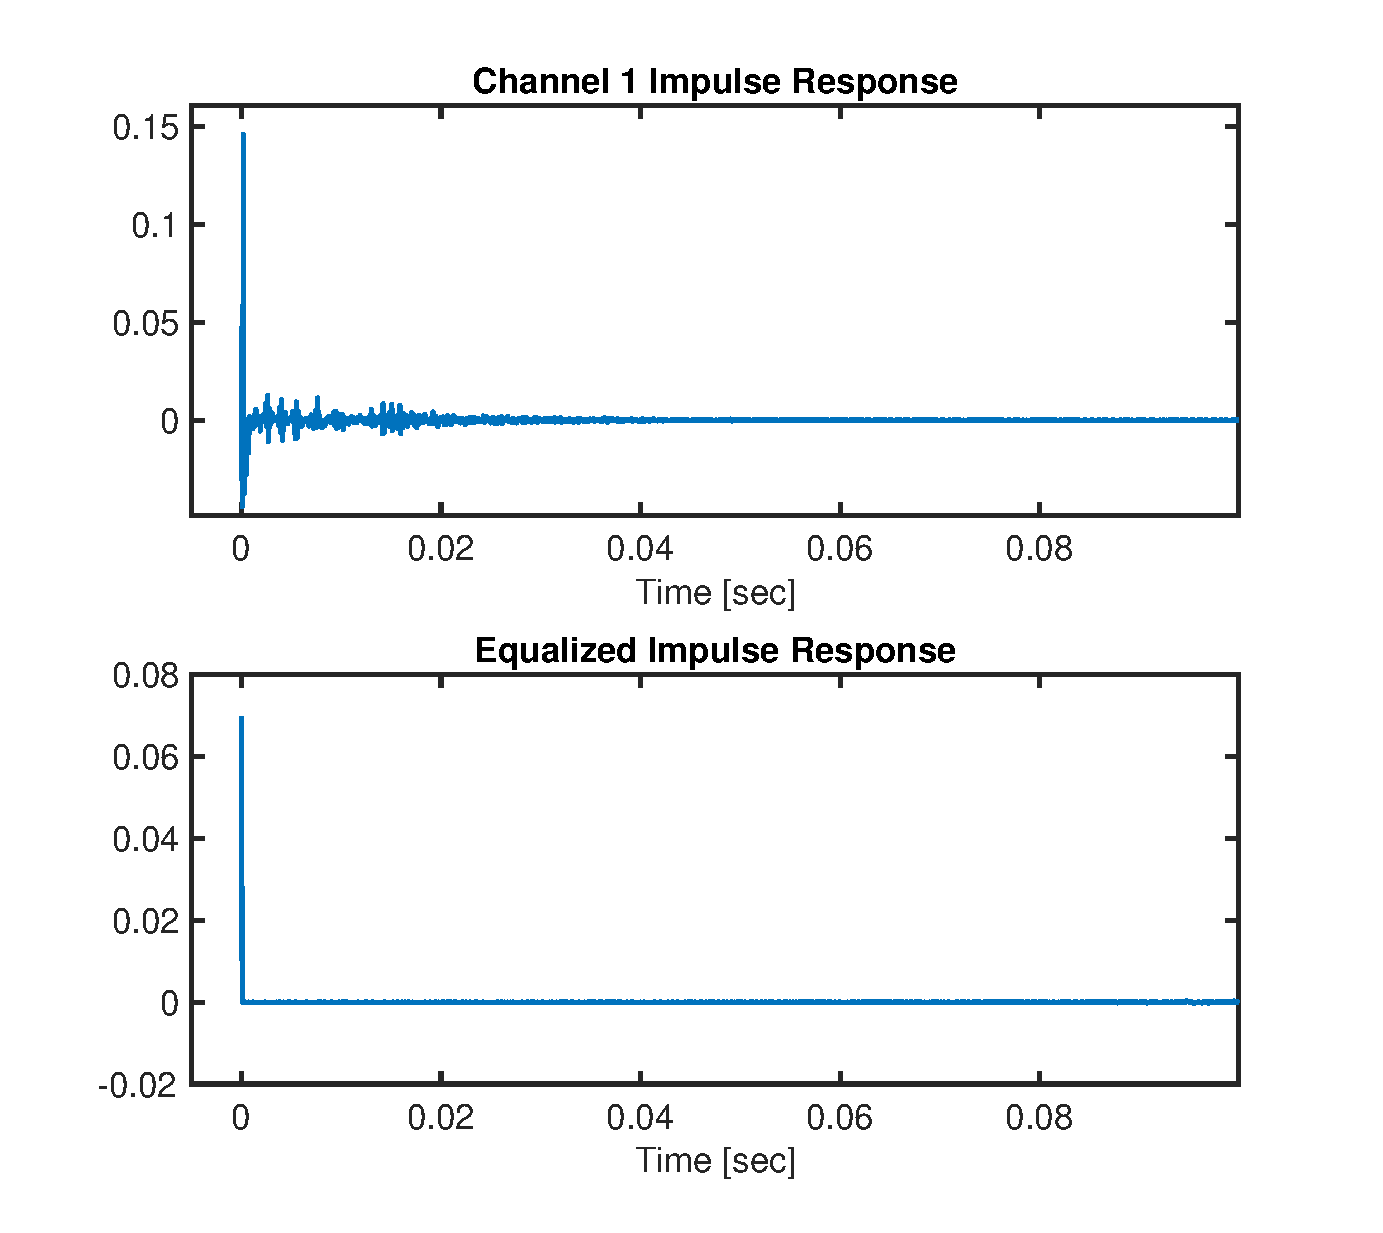
\includegraphics[width=\linewidth]{EIR_p1_based_on_p2}
			\end{subfigure}
			\hfill
			\begin{subfigure}[t]{0.49\textwidth}
				\centering
				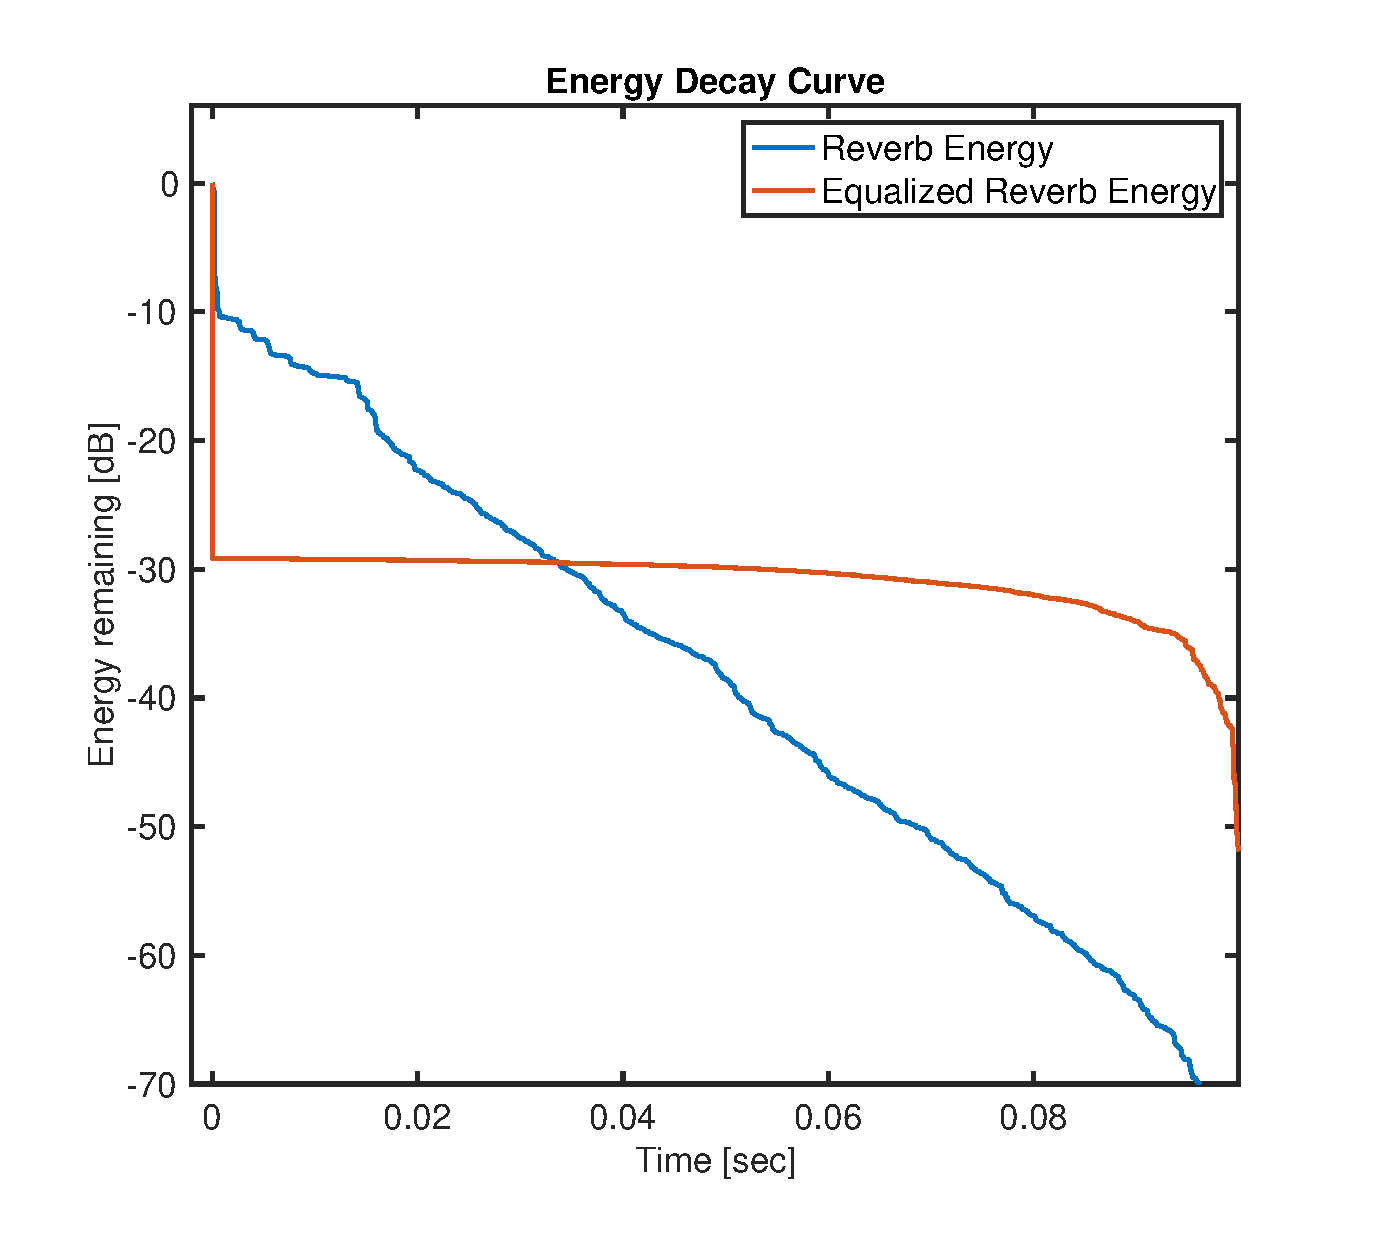
\includegraphics[width=\linewidth]{EDC_p1_based_on_p2}
			\end{subfigure}
		\end{minipage}
	}
	% Dummy subfigure for referencing row C
	\refstepcounter{subfigure}
	\label{subfig:params_p1_compare:C}
	
	\vspace{1em}
	
	% ROW D
	\makebox[\textwidth][l]{%
		\begin{minipage}{0.23\textwidth}
			\centering
			\raggedleft{\footnotesize \textbf{(d)} \newline $p_1 = 3200$ \newline ($p_1 = 2 \cdot p2 \cdot \left(M-1\right)$)} \\
		\end{minipage}%
		\begin{minipage}{0.66\textwidth}
			\begin{subfigure}[t]{0.49\textwidth}
				\centering
				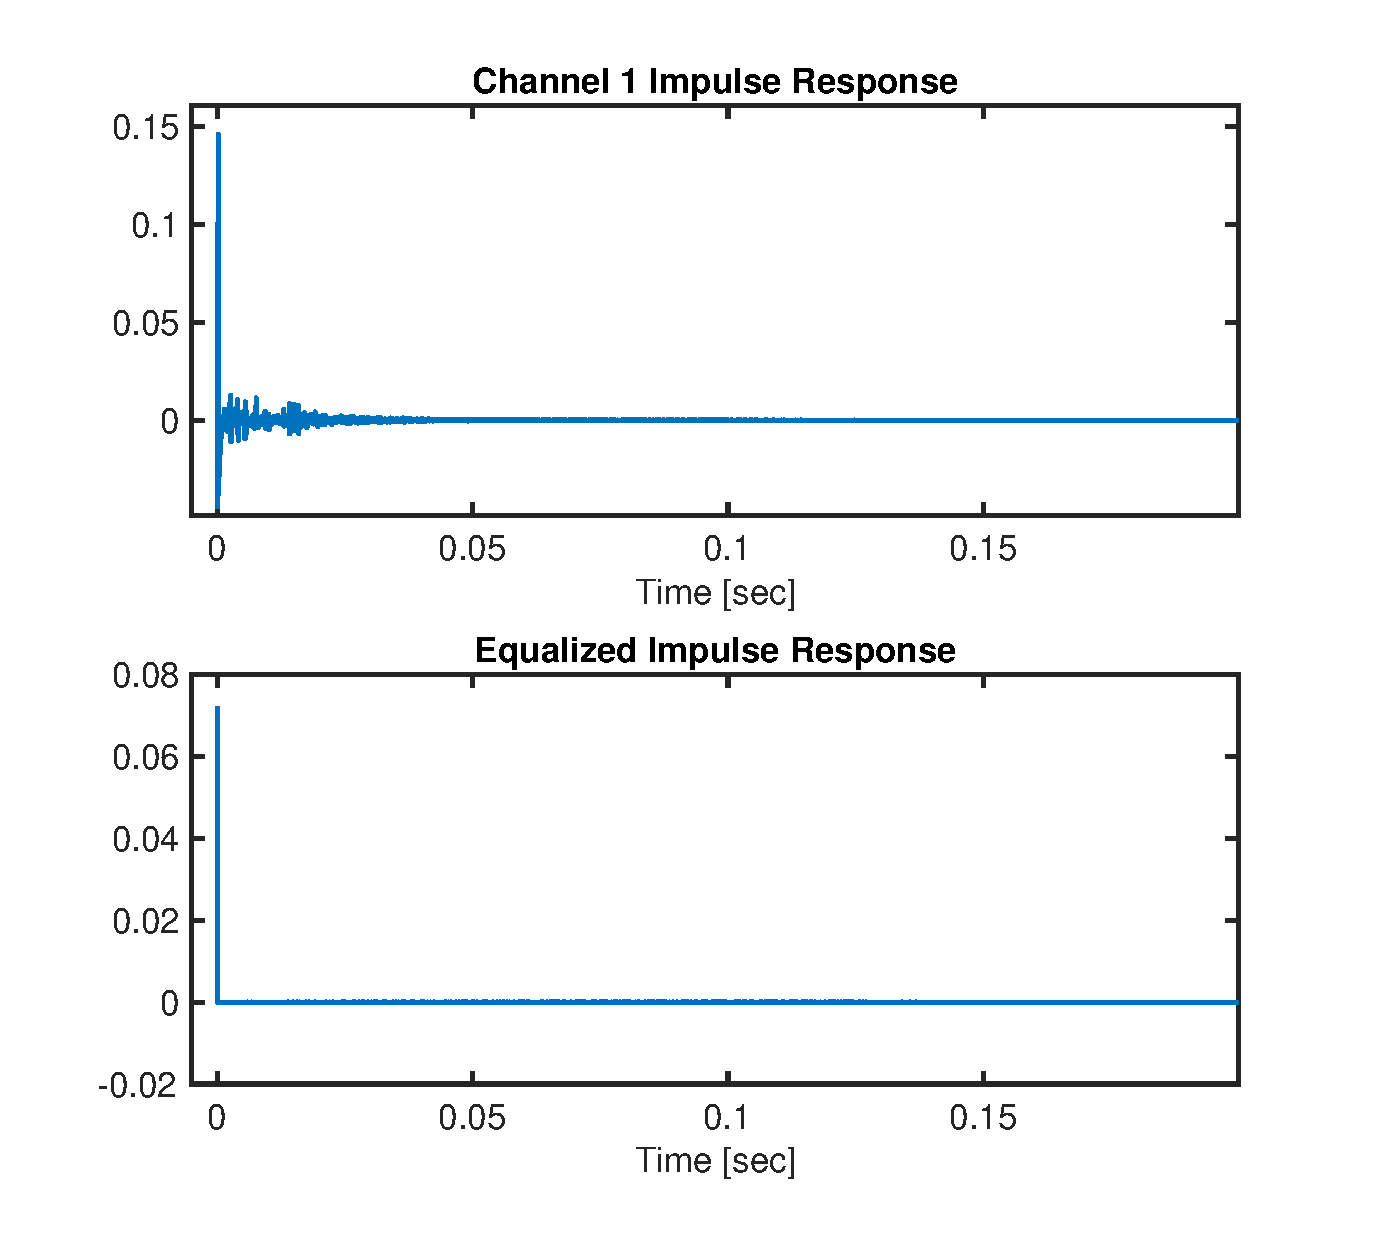
\includegraphics[width=\linewidth]{EIR_p1_2x_p2}
			\end{subfigure}
			\hfill
			\begin{subfigure}[t]{0.49\textwidth}
				\centering
				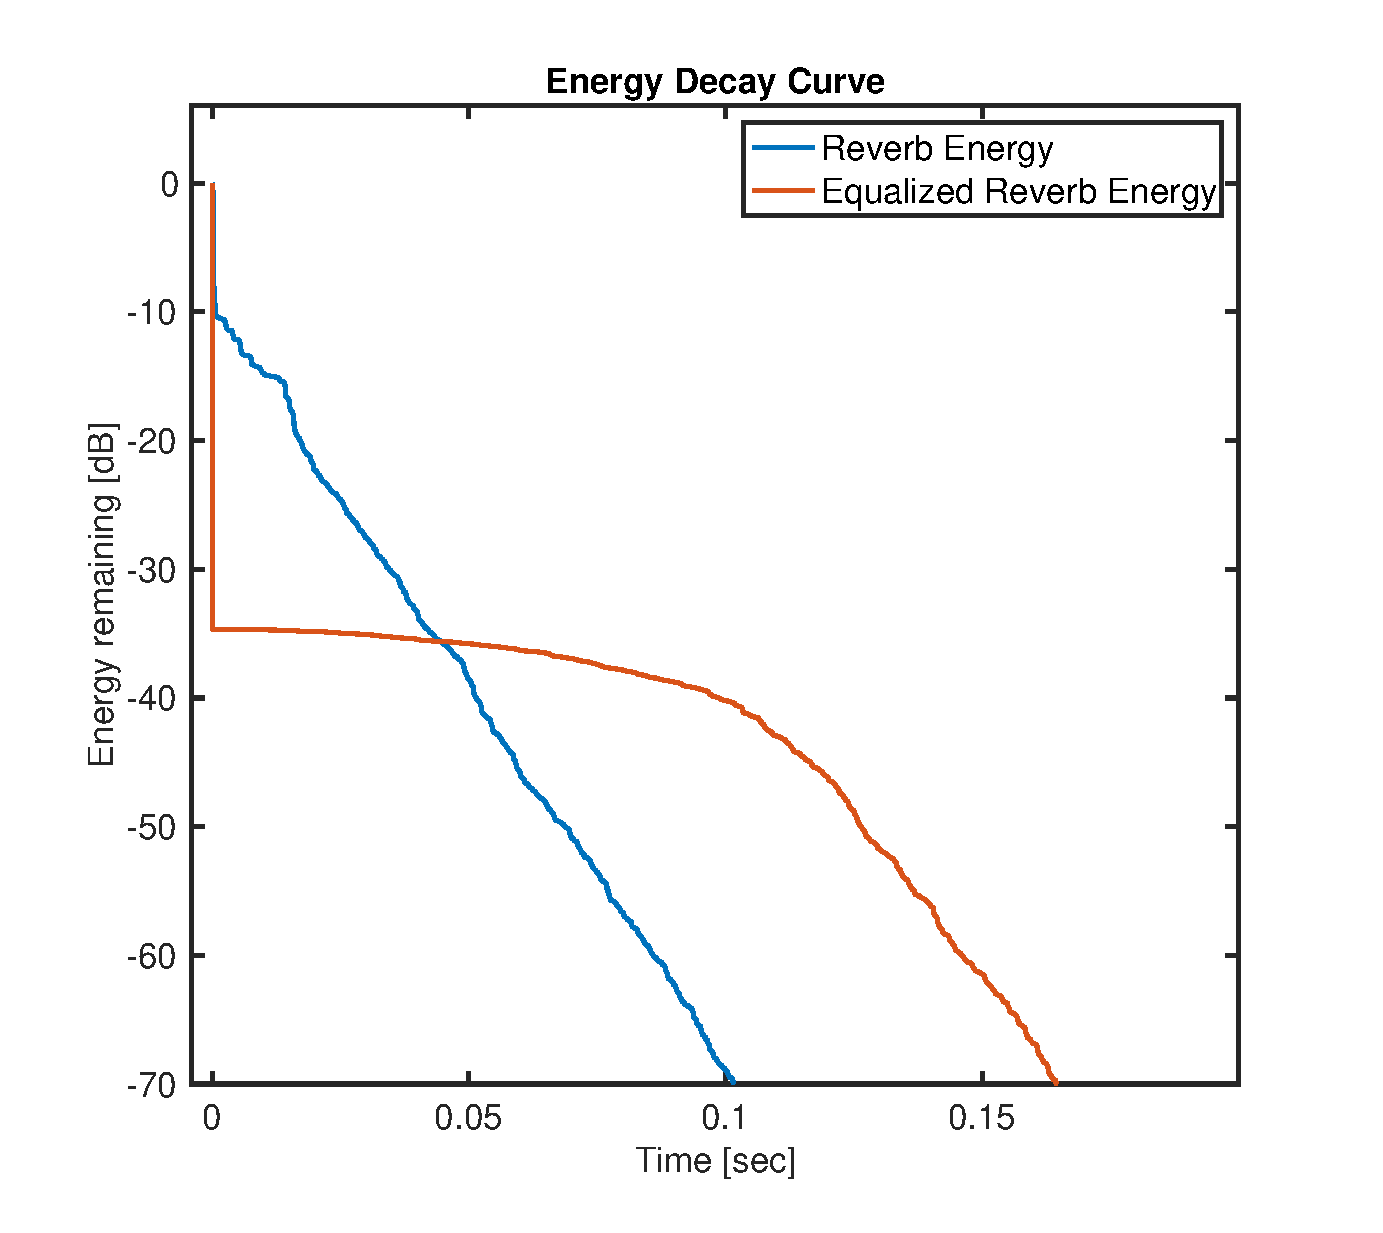
\includegraphics[width=\linewidth]{EDC_p1_2x_p2}
			\end{subfigure}
		\end{minipage}
	}
	% Dummy subfigure for referencing row D
	\refstepcounter{subfigure}
	\label{subfig:params_p1_compare:D}
	
	\caption{Delay-and-Predict dereverberation performance with various source whitening prediction orders ($p_1$) relative to the multichannel linear prediction order, $\mathrm{p2} = \mathrm{N60} / \left(M-1\right)$}
	\label{fig:params_p1_compare}
	
\end{figure}

It was noted that the algorithm provides very little reverberation cancellation for low source-whitening prediction orders, and that reverberation attenuation plateaus around \qty{35}{\decibel} when the source-whitening prediction order rises above approximately $p_1 = 1.25 \cdot p_2 \cdot (\left(M-1\right)$. This demonstrates the importance of the matching (or exceeding) the spectral resolution of the source-whitening stage to the effective spectral resolution of the MC-LP stage. This makes intuitive sense since any AR characteristics of the source that are visible within the spectral resolution the MC-LP analysis which have not been removed by the source-whitening stage, will be captured in the MC-LP analysis and thus will distort the estimate of the true system inverse.

\section{Blind Deconvolution Performance}

To analyze the behaviour of the full blind dereverberation algorithm (i.e., blindly estimating the source AR properties), the same parameters and test conditions were used to compare the performance of the MINT equalizer (Figure \ref{fig:fullExample_MINT}), the DAP equalizer generated using a source-whitening filter trained on clean speech(Figure \ref{fig:fullExample_NotBlind})), and the blind DAP equalizer (Figure \ref{fig:fullExample_Blind}). 

The source signal used was a \qty{60}{\sec} sample of a male talker (namely the entire "MKLS0" collection from the TMIT database, synthetically looped to \qty{60}{\sec}), and the RIR was a 4-channel \qty{1}{\sec} T60 generated by exponentially windowing the MYRiAD SAL RIR measurement as before. The MC-LP order was set to $p_2 = 1.25 \cdot N60 / \left(M-1\right)=6667$ and the source-whitening prediction order was set to $p_1 = 1.25 \cdot p_2 \cdot \left(M-1\right)=25001$. The spectrogram plots were generated using a different signal than the one used in training (namely "SA2" \textbf{TBD which collection/talker} from the TMIT database). This was done to emphasize the potential that the "over-whitening" of the training source signal may lead to an added reverberant effect when the equalizer is applied to a different signal (as described in Section \ref{section_dap}).

% Test Conditions:
% - Source Signal = TMIT_MKLS0.WAV
% - Source length = 960000
% - RIR = MYRiAD SAL Measured RIR (T60 = 2100 msec, Truncated Exponentially to T60 = 1000 msec)
% - RIR length = 32000
% - T60 = 1000 msec (N60 = 16000 samples)
% - SNR = 300 dB
% - Noise Signal = office ventilation
% - SIR = Inf dB 
% - Interference Signal = None
%
% Delay-and-Predict config:
% - Number of Microphones (M) = 4
% - Source whitening order (p1) = 25001 (1.25 * p2 * (M-1))
% - Multichannel Linear Prediction order (p2) = 6667 (1.25 * N60 / (M-1))
% - Source whitening Enabled? = 1
% - Source whitening on clean speech? = varied

\begin{figure}[H]
	\centering
	\begin{subfigure}[b]{0.38\textwidth}
		\centering
		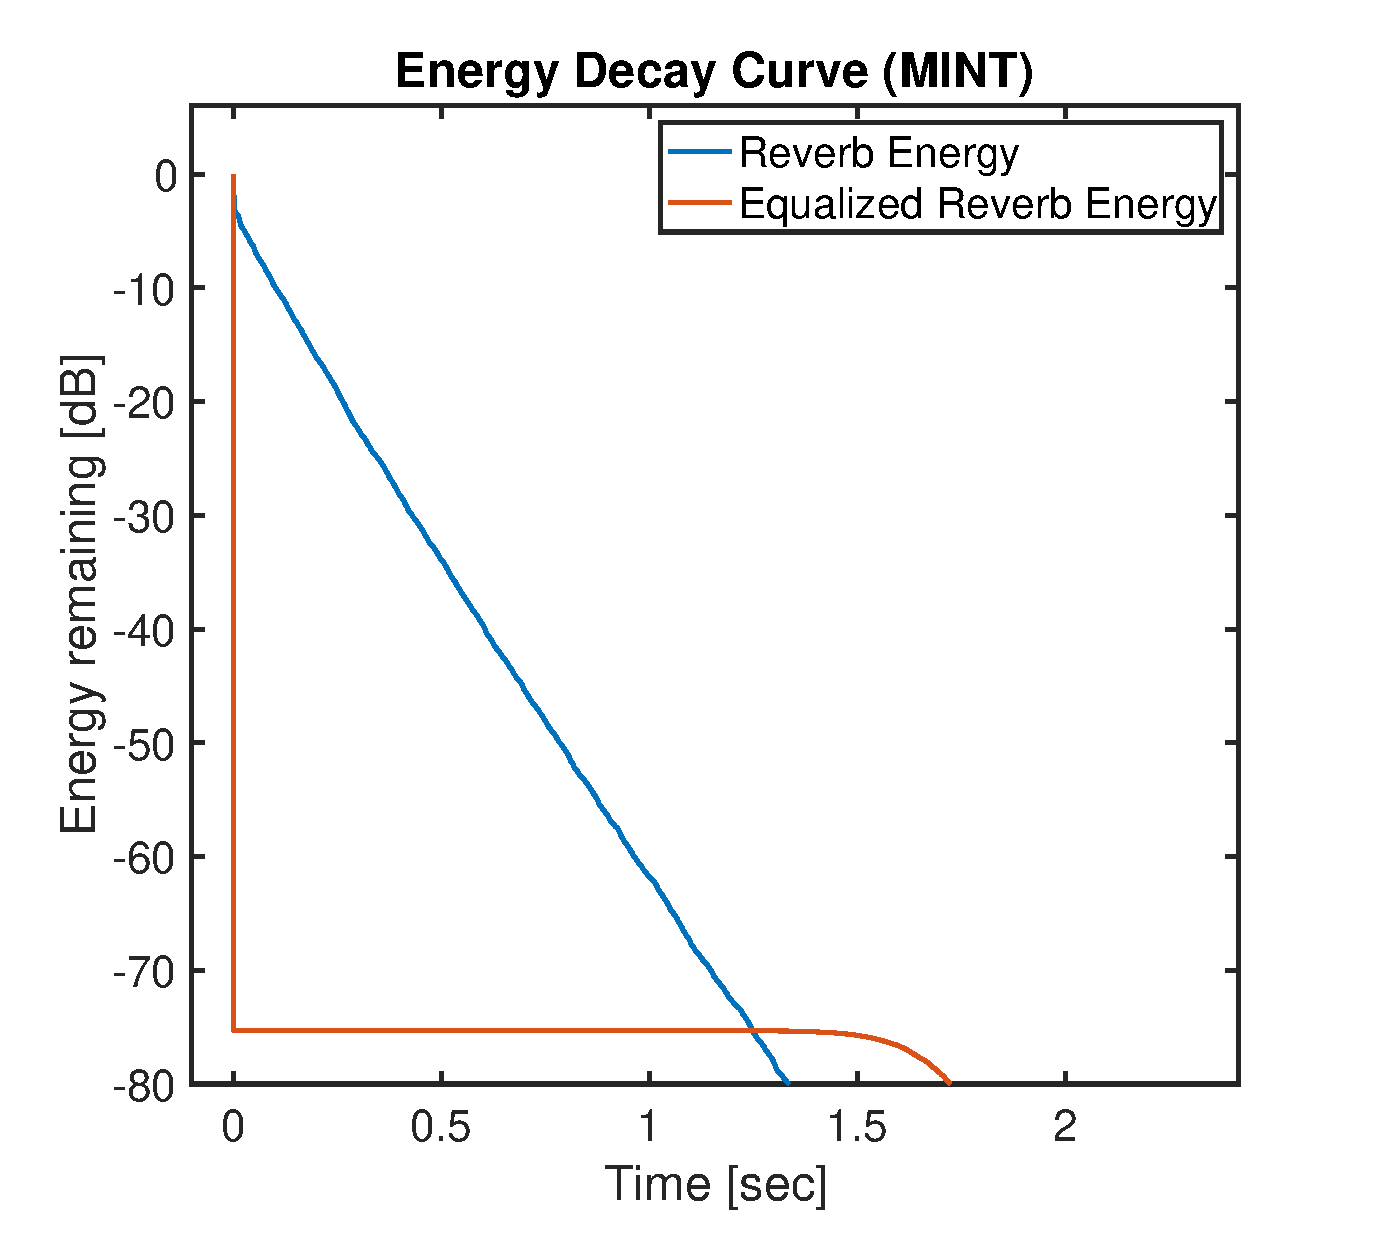
\includegraphics[width=\textwidth]{FullExample_MINT_EDC}
	\end{subfigure}
	\begin{subfigure}[b]{0.49\textwidth}
		\centering
		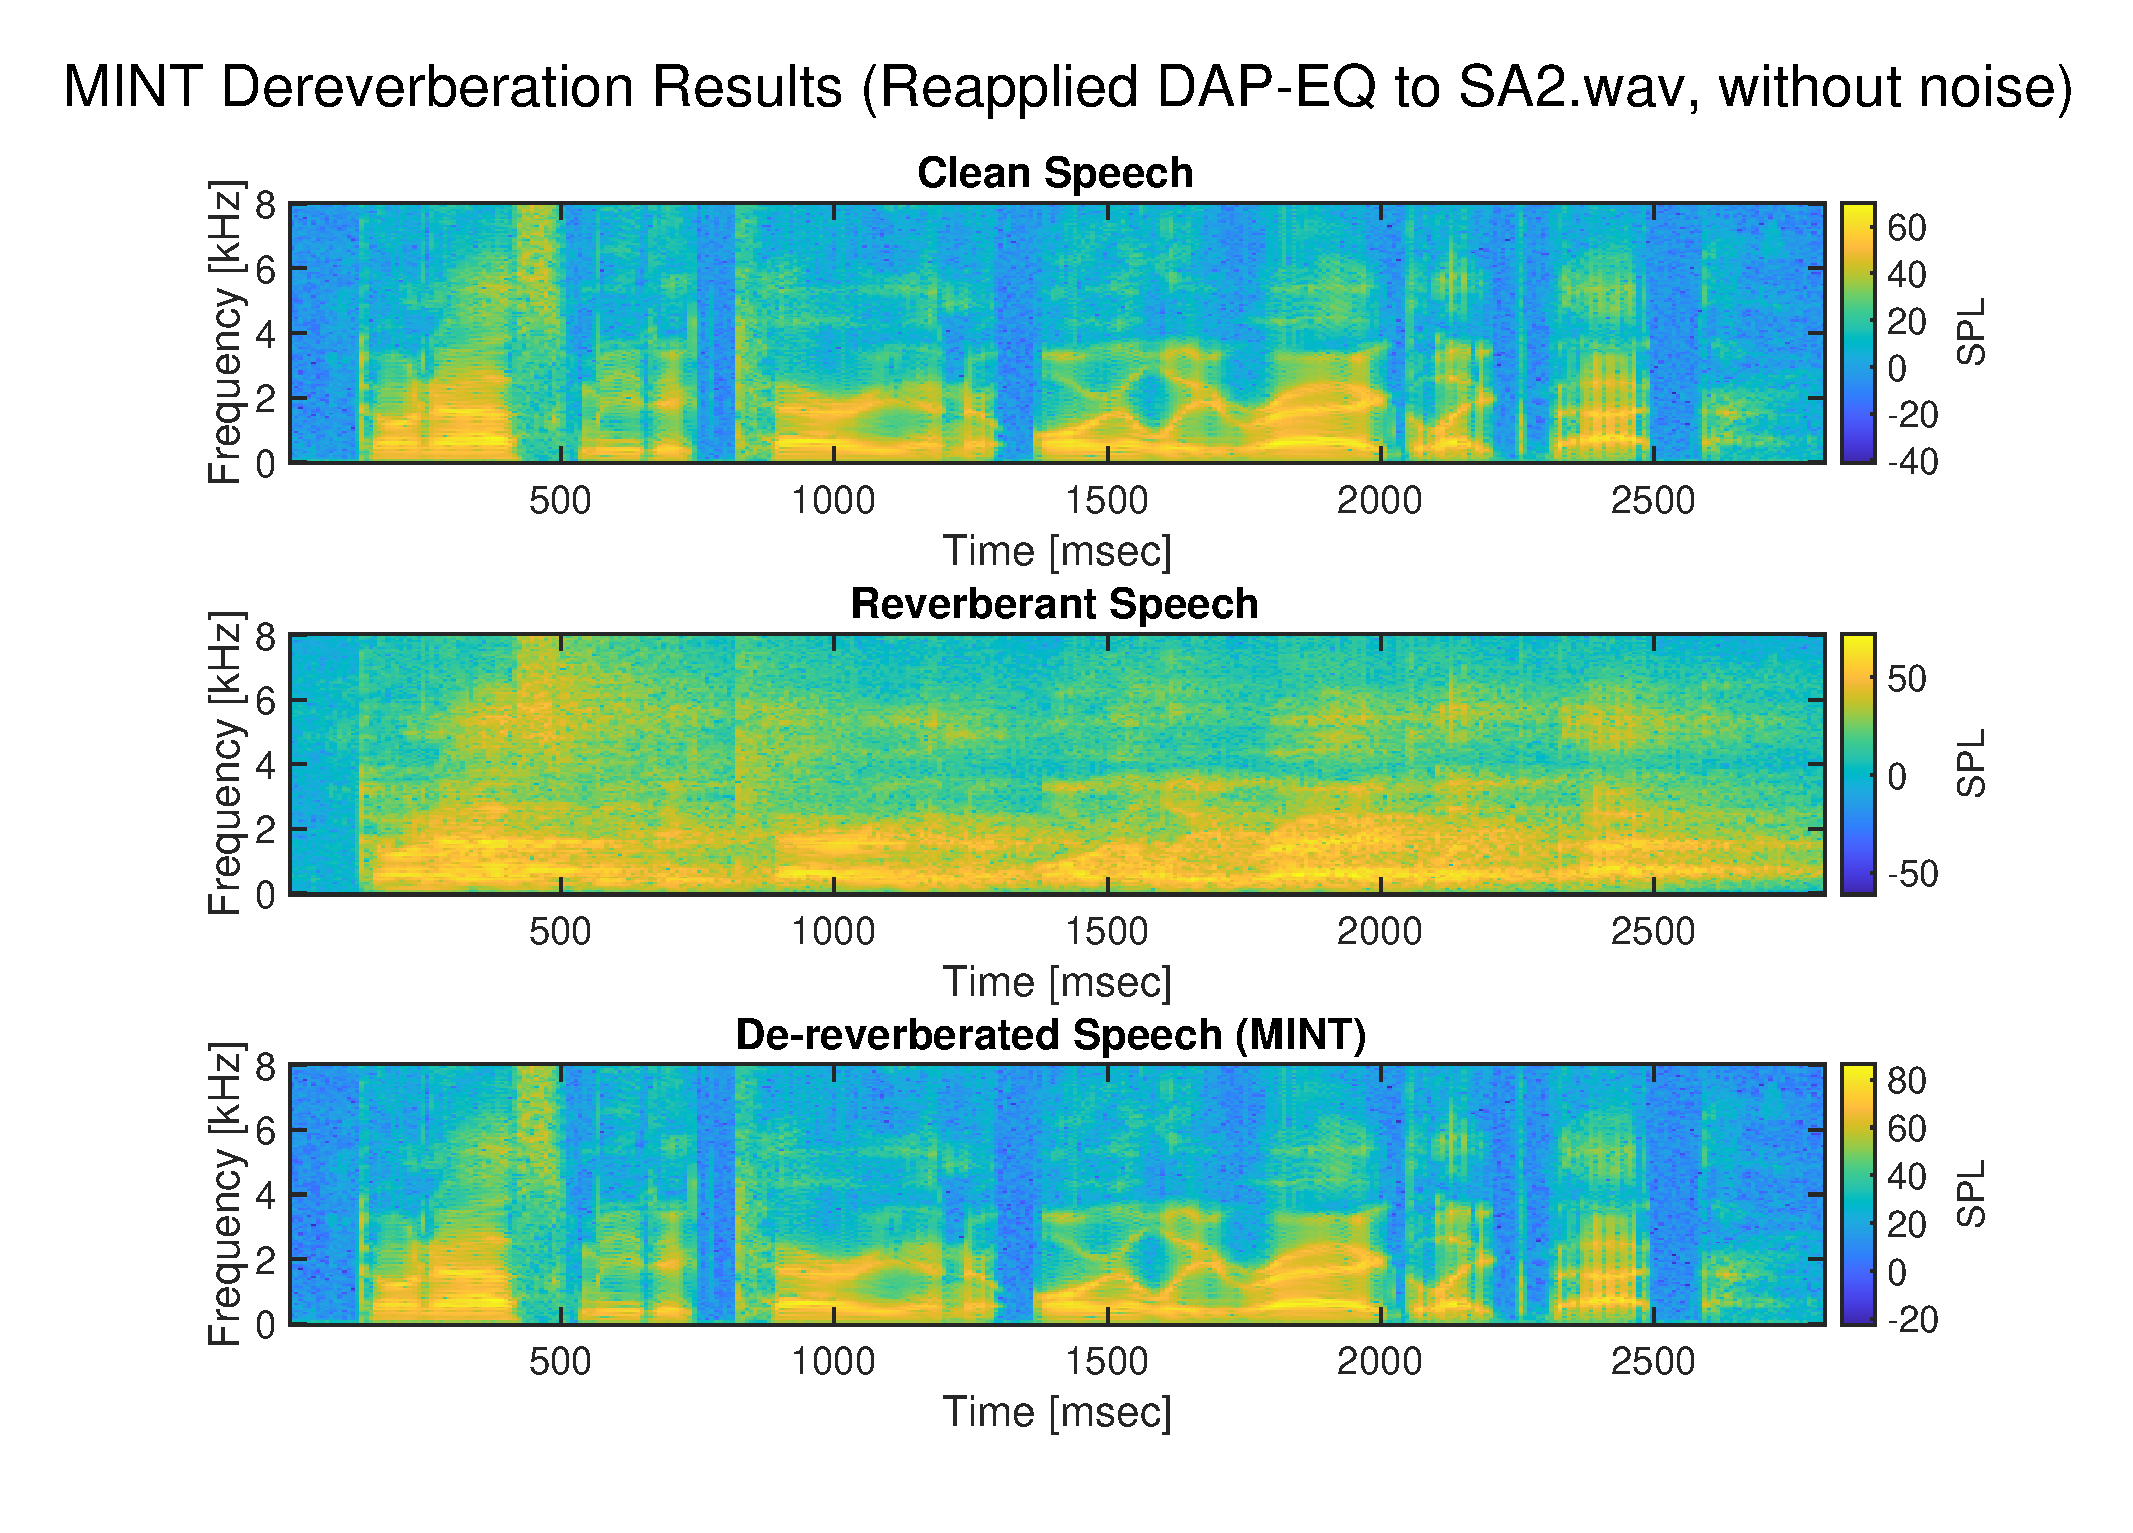
\includegraphics[width=\textwidth]{FullExample_MINT_Spectrogram}
	\end{subfigure}
	\caption{MINT Equalizer performance (EDC and Spectrogram)}
	\label{fig:fullExample_MINT}
\end{figure}


\begin{figure}[H]
	\centering
	\begin{subfigure}[b]{0.38\textwidth}
		\centering
		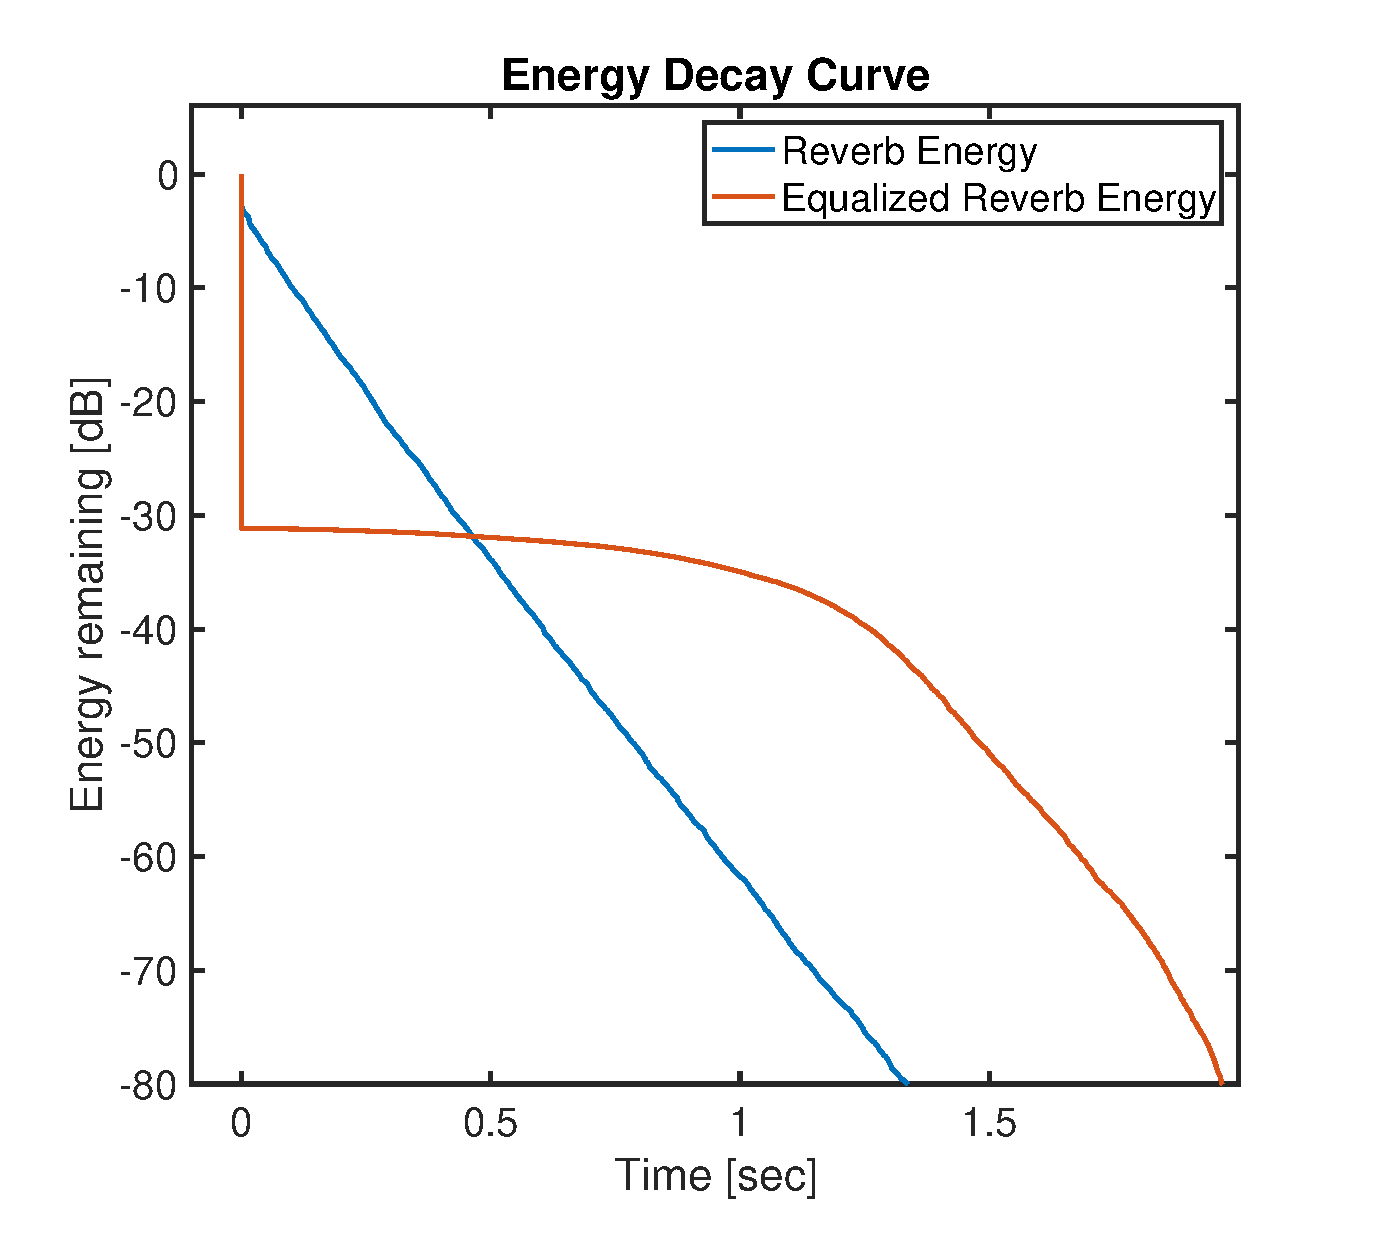
\includegraphics[width=\textwidth]{FullExample_NotBlind_EDC}
	\end{subfigure}
	\begin{subfigure}[b]{0.49\textwidth}
		\centering
		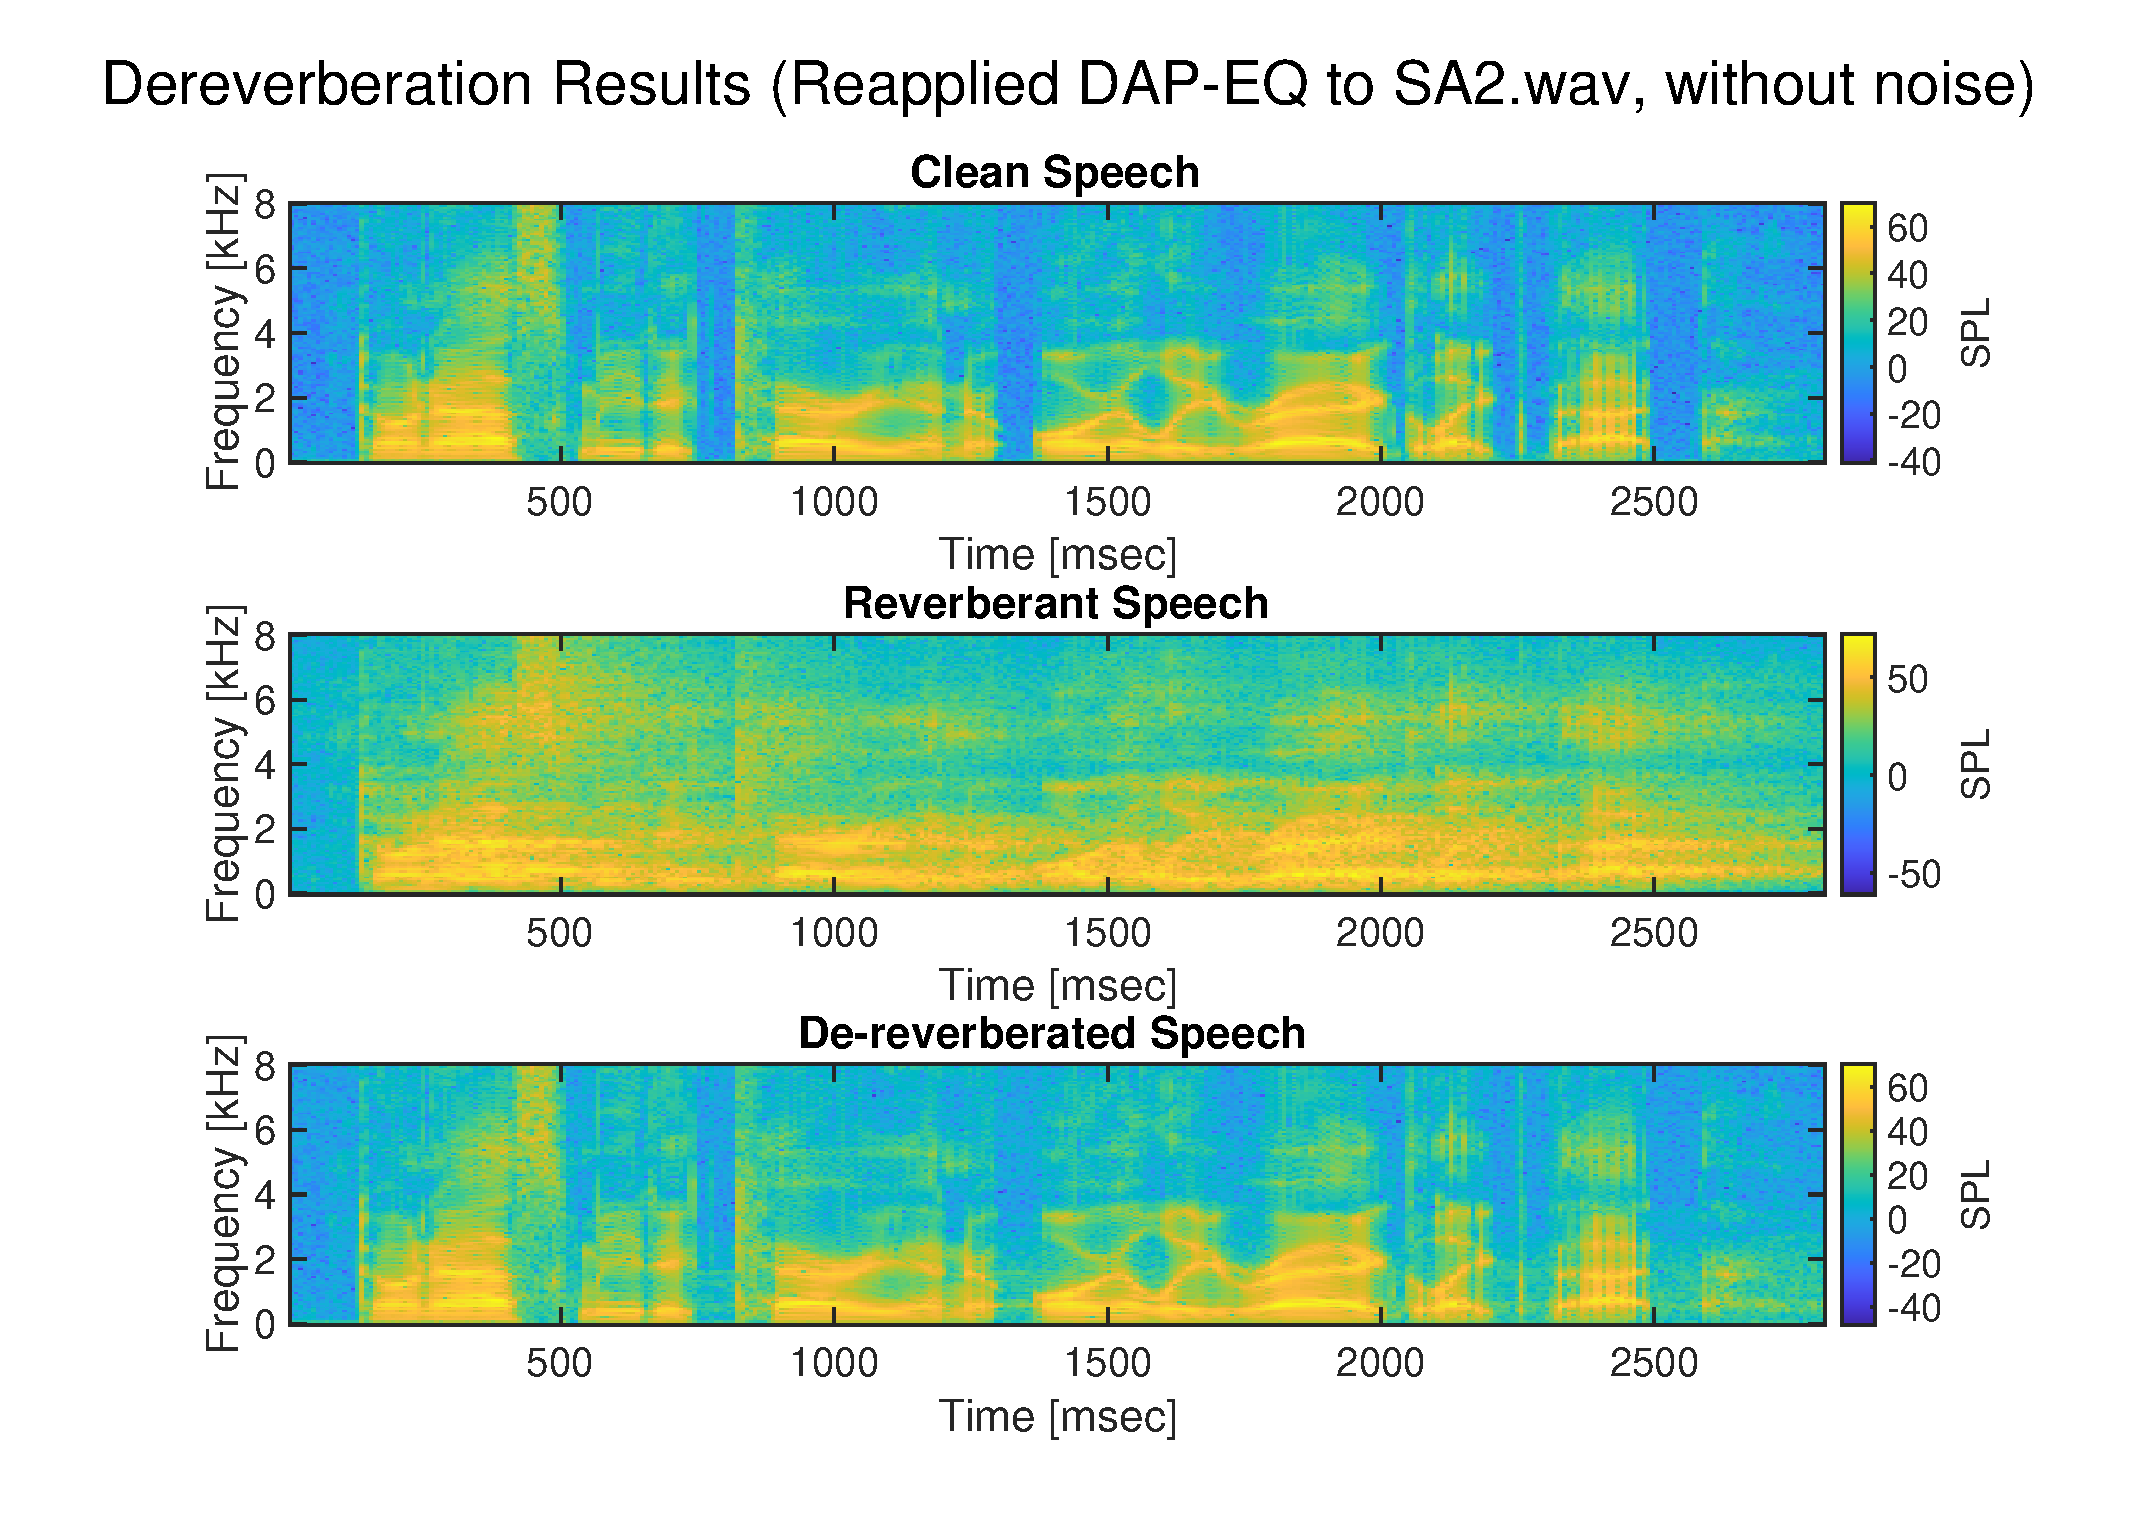
\includegraphics[width=\textwidth]{FullExample_NotBlind_Spectrogram}
	\end{subfigure}
	\caption{Delay-and-Predict Equalizer performance (EDC and Spectrogram) with the source-whitening filter computed using clean speech (i.e., not blind)}
	\label{fig:fullExample_NotBlind}
\end{figure}


\begin{figure}[H]
	\centering
	\begin{subfigure}[b]{0.38\textwidth}
		\centering
		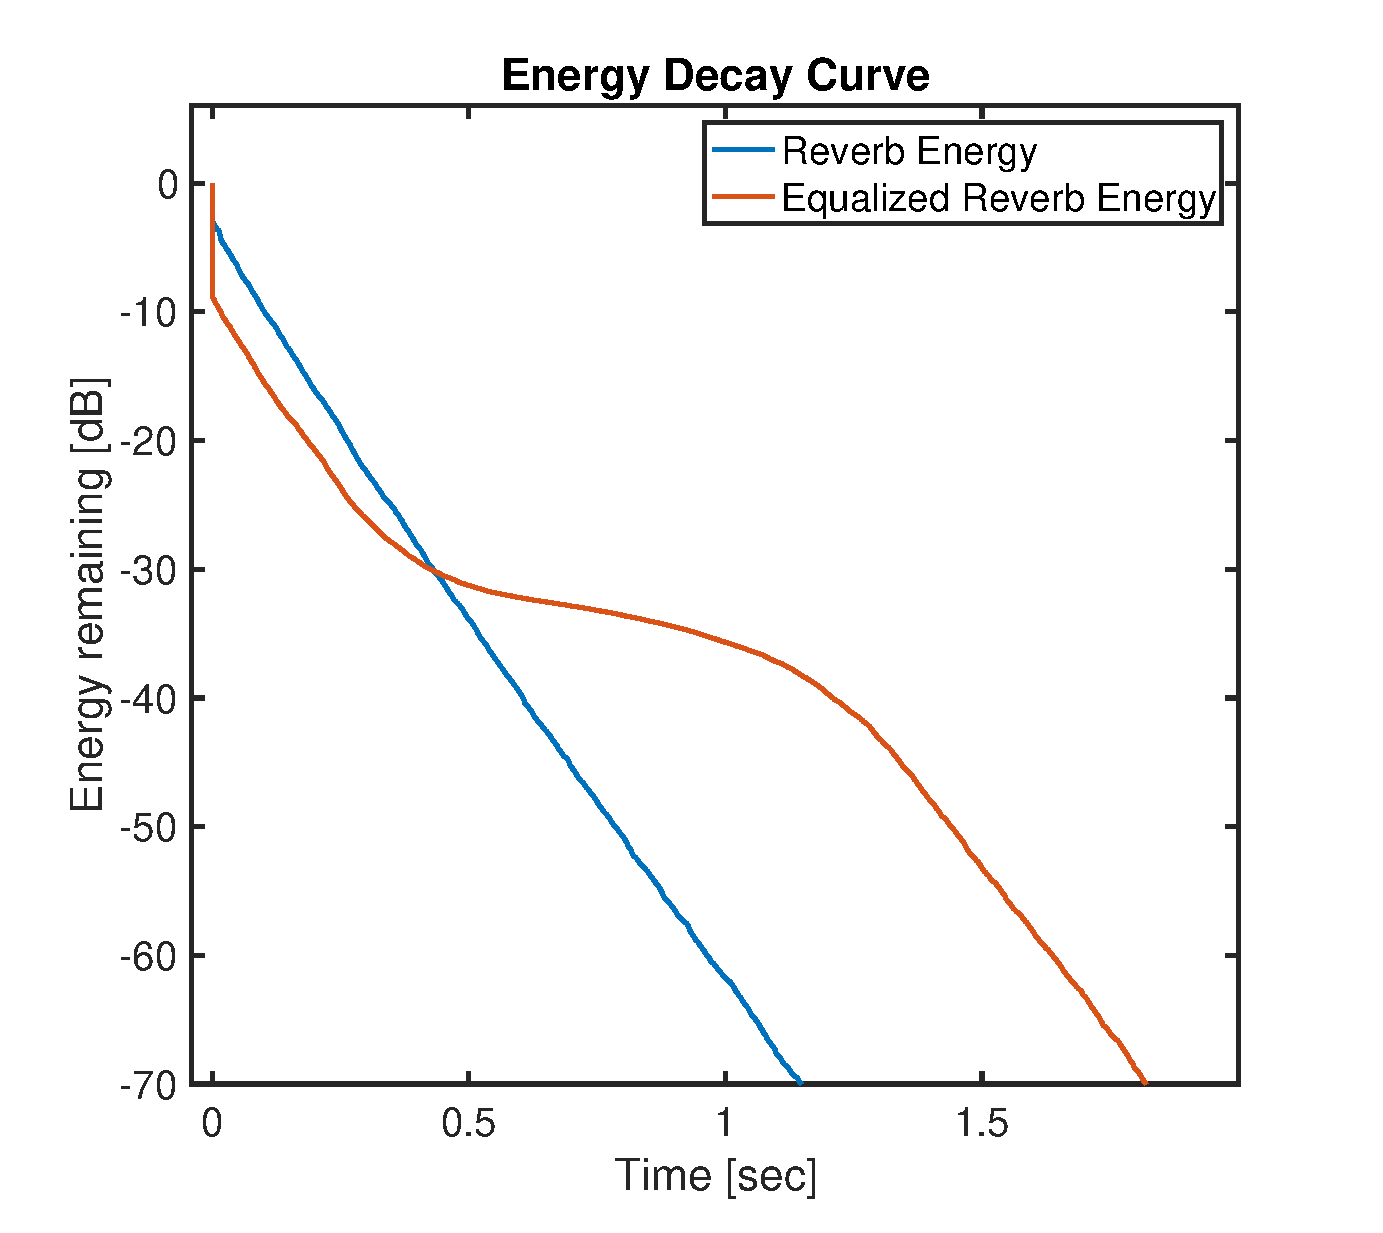
\includegraphics[width=\textwidth]{FullExample_Blind_EDC}
	\end{subfigure}
	\begin{subfigure}[b]{0.49\textwidth}
		\centering
		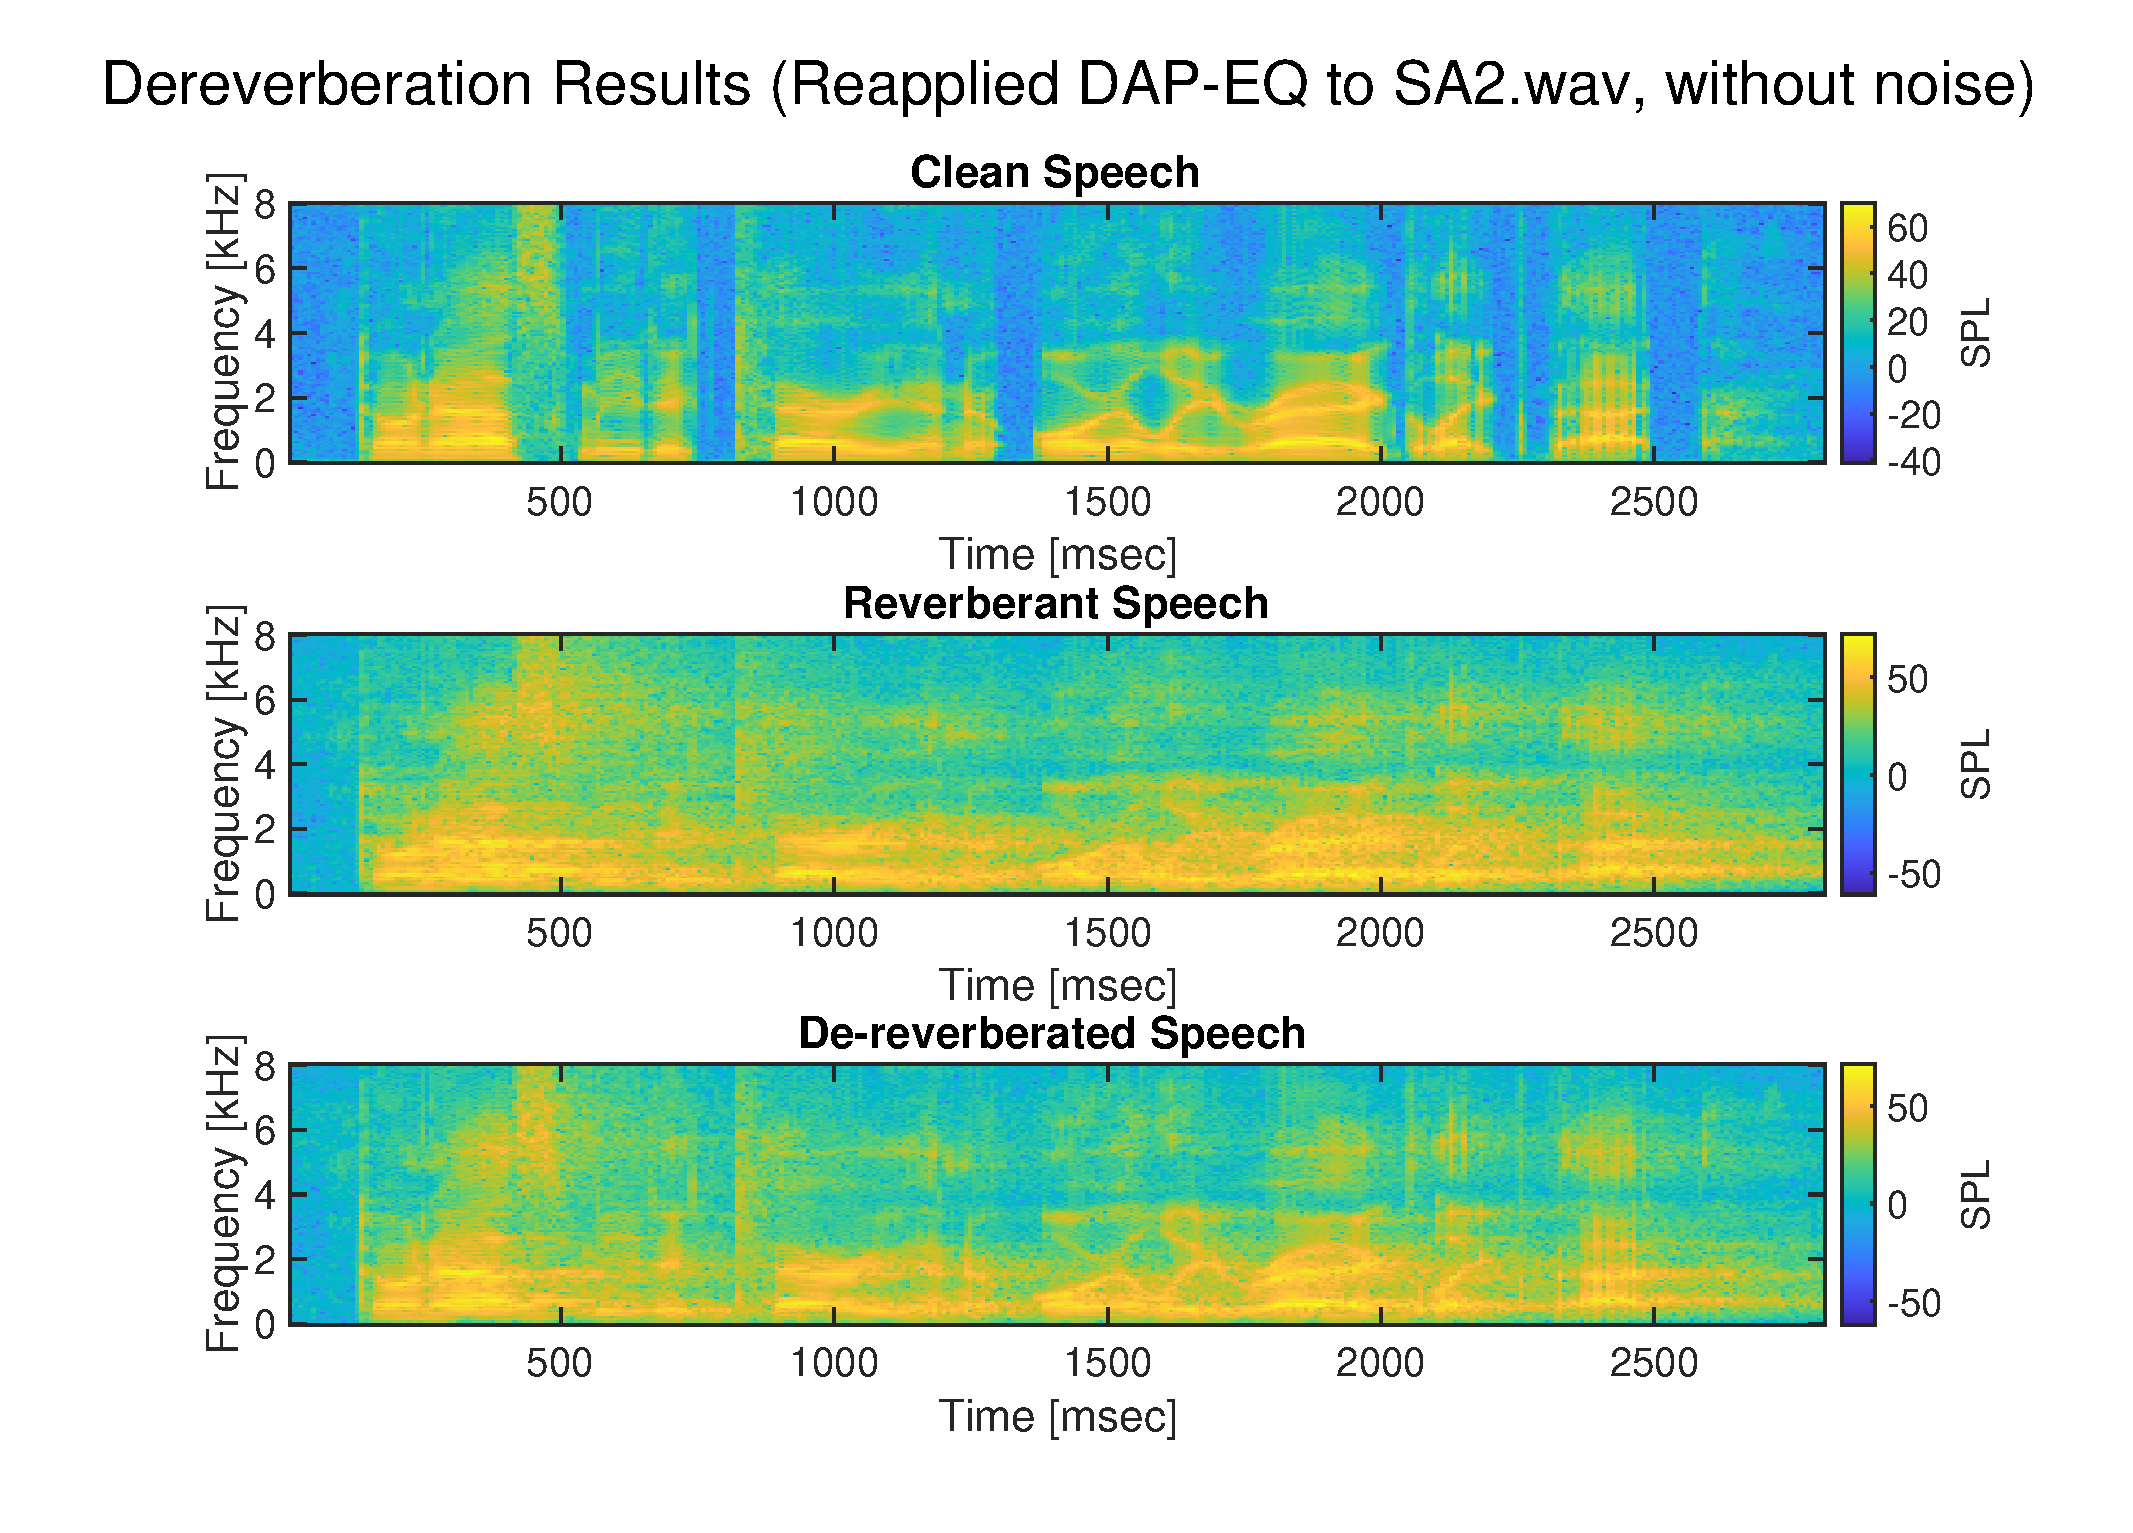
\includegraphics[width=\textwidth]{FullExample_Blind_Spectrogram}
	\end{subfigure}
	\caption{Delay-and-Predict Equalizer performance (EDC and Spectrogram) with the source-whitening filter computed using reverberant speech (i.e., blind)}
	\label{fig:fullExample_Blind}
\end{figure}

As observed before, the MINT equalizer and the DAP equalizer trained on clean speech both produce EDCs that show a nearly instanteously decay by a substantial amount. As before, the EDC corresponding to the DAP equalizer trained on clean speech plateaus around 30-35 \unit{\decibel} and remains roughly flat over the time spanned by the equalizer length, and falls off at the end due to increased estimation variance at longer autocorrelation lags.

The EDC corresponding to the blind DAP equalizer (Figure \ref{fig:fullExample_Blind}) shows much less attenuation of the early part of the RIR (approximately \qty{6}{\decibel} attenuation). It continues to decay at approximately the same rate as the original RIR, until it plateaus at a similar attenuation of approximately 30-35 \unit{\decibel}, and similarly falls off at the end of the time spanned by the equalizer length. Thus the blind version of the DAP algorithm provides a similar result to the non-blind version, but its performance is degraded by having to blindly estimate the source-whitening filter. The performance degradation was presumed to be due to common or near-common AR parameters (i.e., the effective poles) between the acoustic channels since RTFs tend to have some similarity in their frequency response, and due to the finite number of spatial sampling points (i.e., microphones) being used to average out the non-common AR parameters in the estimation of the source-whitening filter (i.e., Equation \ref{eq:dap_avg_autocorr}).

Looking at the spectrogram results, a clear benefit of all three equalizers was noted. For example, note that the diphthong around \qty{1500}{\milli\sec}, is almost completely obsecured by the smearing of reverberant energy (row 2), whereas it is more clearly defined in the spectrogram of the dereverberated speech signals (row 3). While this improvement is less pronounced in the blind DAP case than the MINT or supervised DAP cases, there is still a clear benefit of the algorithm.




\section{Source Properties}

Two properties of the source speech stimulus were analyzed: source data length (i.e., length of the source sequence), and its spectral colouration. It was hypothesized that larger amounts of source data would decrease variance in the estimation of autocorrelation values for usage in the normal equations for both linear prediction stages, improving performance. It was also hypothesized that the amount of colour (i.e., the "peakiness") of the source spectrum would have a negative impact on performance due to the increased demand on the source-whitening stage, and due to the known fact that the condition number of autocorrelation matrices is proportional to the signals spectral dynamic range which results in worse-conditioned normal equations.

Since the power spectrum of a signal generally becomes smoother as sequence length increases, the evaluation method had to be designed carefully to isolate these two properties.  

In all cases, the 4-channel RIR was the "SAL" room from the MYRiAD database, exponentially windowed to $\mathrm{T60} = 100 \unit{\milli\second}$, $p_2 = \mathrm{N60} / \left(M-1\right)$, and $p_1 = 2 \cdot p_2 \cdot \left(M-1\right)$. The fully blind DAP algorithm was used in this evaluation


\subsection{Source Data Length}

To test the source data length, the same \qty{3.6}{\sec} speech sample ("SA1" from the TMIT database, \textbf{TBD which talker}) was used in each test case, and was looped synthetically (1, 2, 3 and 4 times respectively) to the desired data length. In this way, the data length was increased without changing the spectrum. The results for each case are shown in Figure \ref{fig:params_source_length_compare}. The first column shows the performance of the source-whitening stage. The equalized RTF results (second column) show the equalized magnitude/phase response generated by taking the fourier transform of the EIR. The third column shows the resulting EDC.

%Test: Same spectrum different length
% -     Blind DAP
% - 	Speech is SA1.wav looped X times
% - 	RIR = SAL truncated to 100 msec = 1600 samples, M = 4 mics
% -     P1 = 2 * p2 * (M-1)
% - 	P2 = N60 / (M-1)
% - 	Reran exact same test for longer source sequences generated by looping SA1 – Exact same spectrum just more data (excludes spectrum dependency)


% Source Data Length Compare, Length = [(1x) 58061,  (2x) 116122, (3x) 174183, (4x) 232244 ], Blind

\begin{figure}[H]
	\centering
	
	% ROW A
	\makebox[\textwidth][l]{%
		\begin{minipage}{0.08\textwidth}
			\centering
			\raggedleft{\footnotesize \textbf{(a)} \newline \qty{3.6}{\sec} \newline source} \\
		\end{minipage}%
		\begin{minipage}{0.91\textwidth}
			\begin{subfigure}[t]{0.32\textwidth}
				\centering
				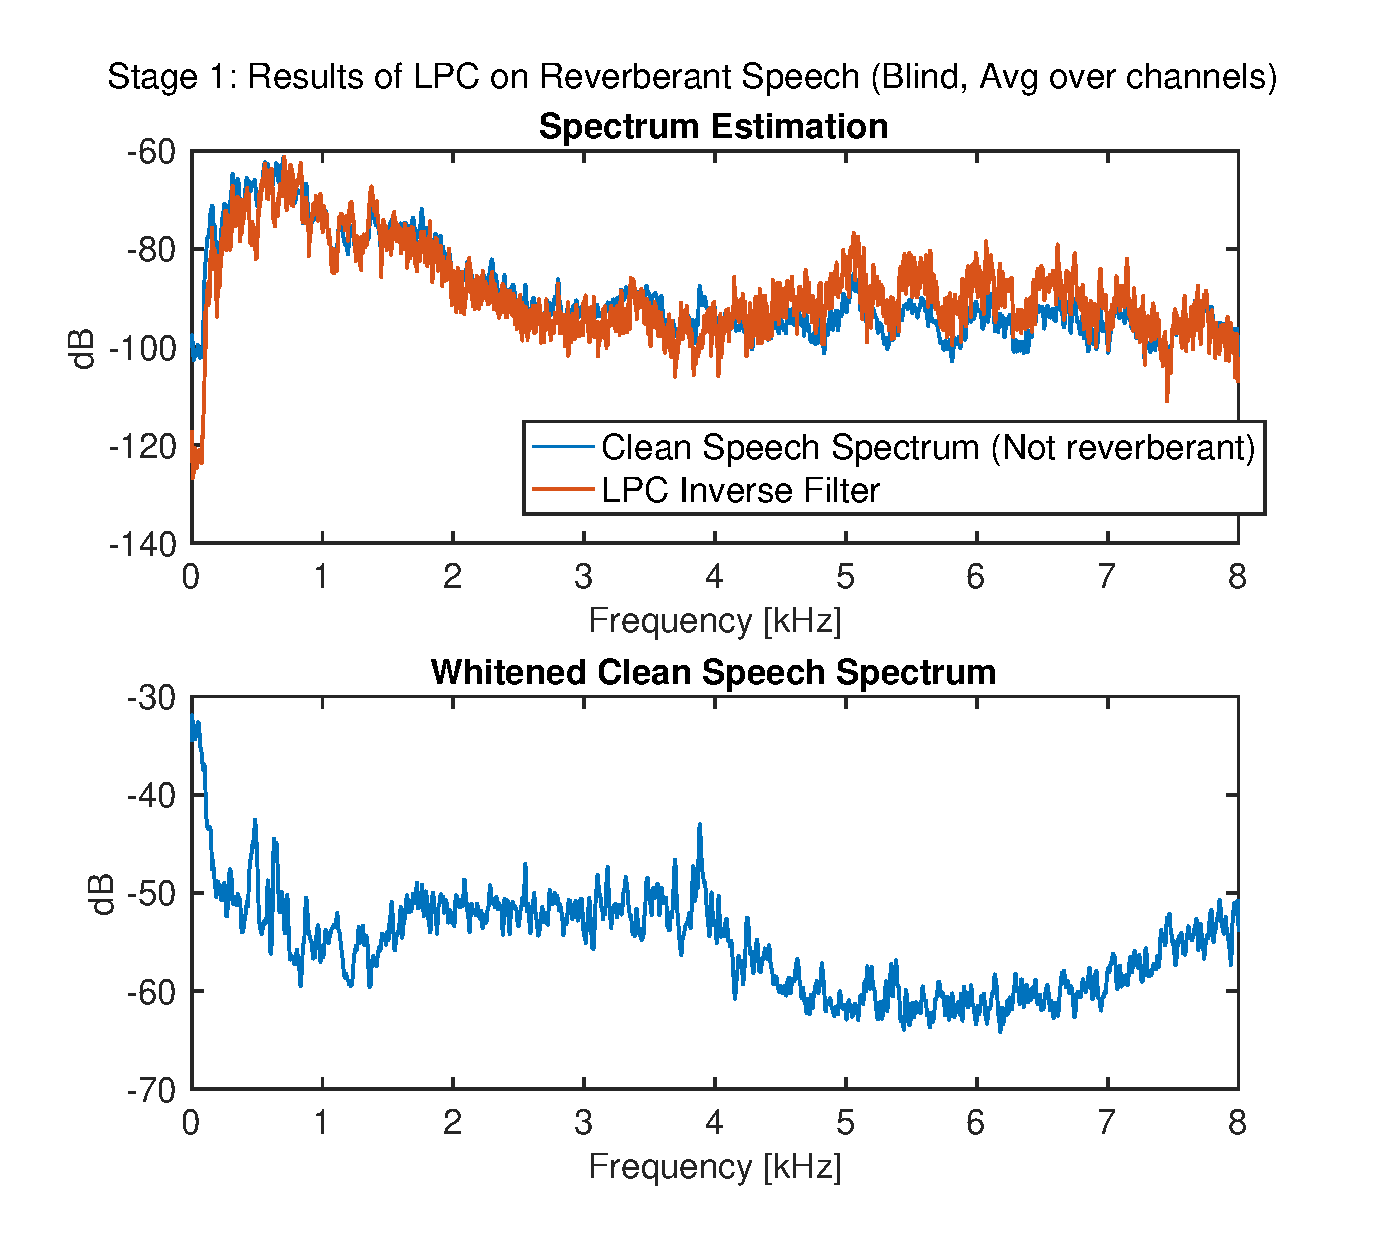
\includegraphics[width=\linewidth]{S1_SourceLength_1_Blind}
			\end{subfigure}
			\hfill
			\begin{subfigure}[t]{0.32\textwidth}
				\centering
				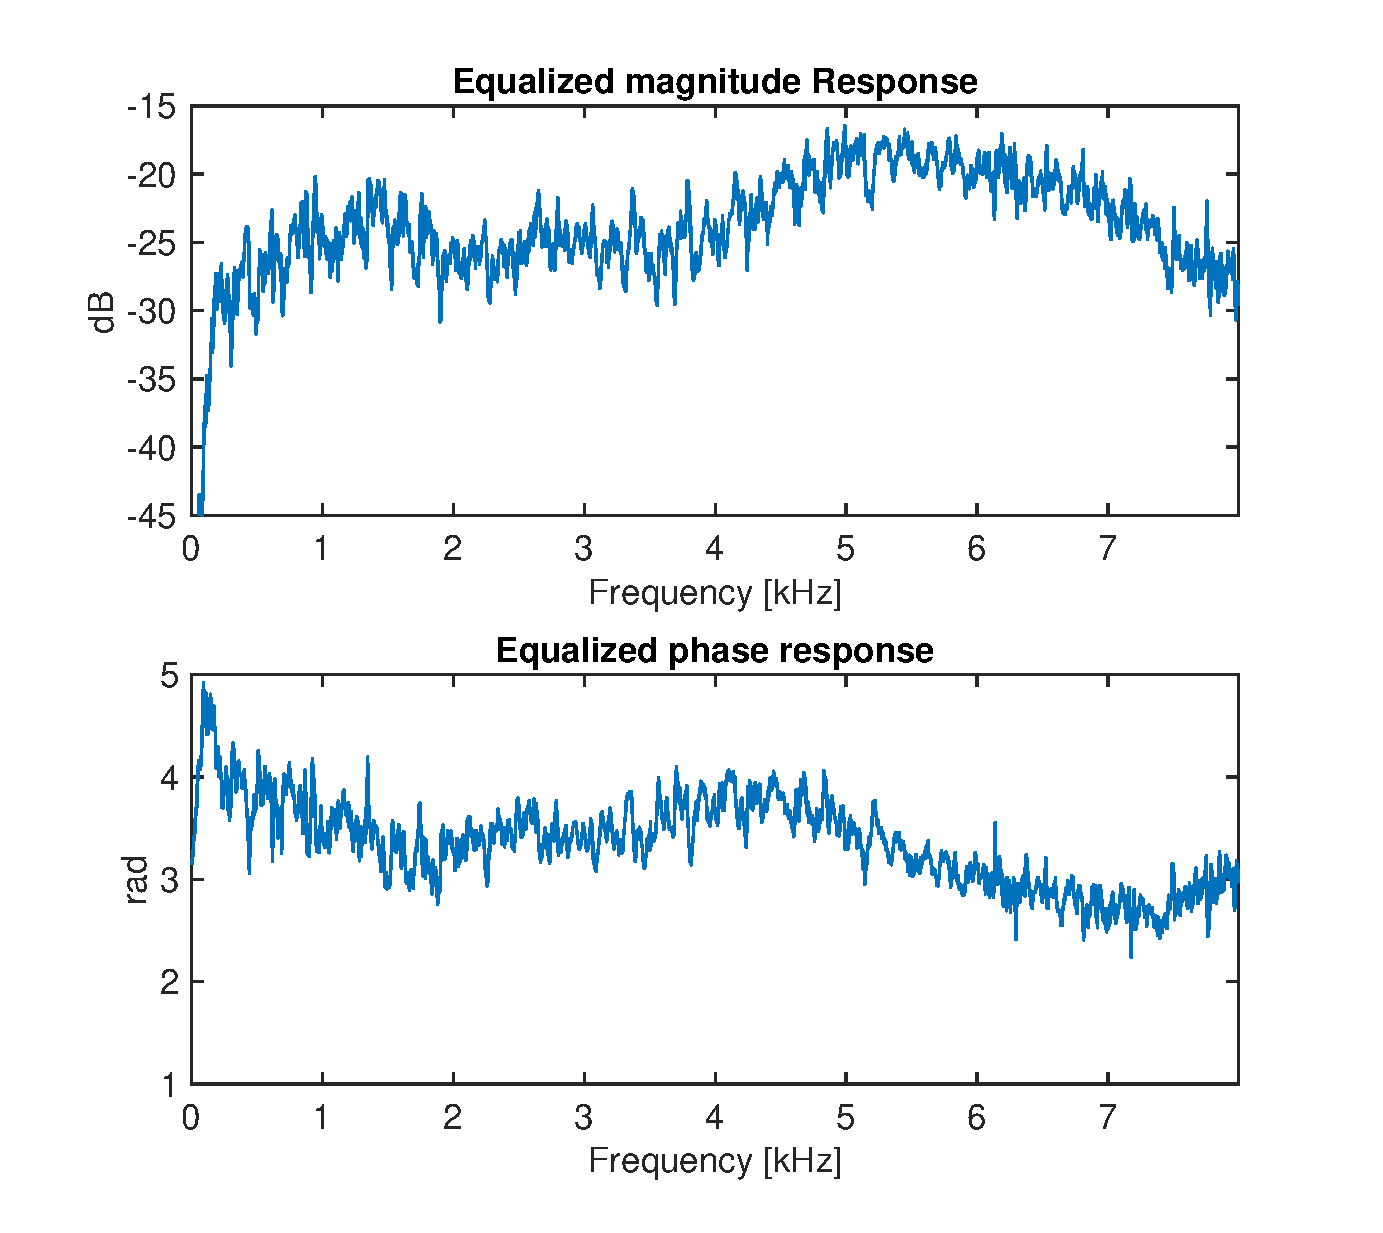
\includegraphics[width=\linewidth]{Equalized_RTF_SourceLength_1_Blind}
			\end{subfigure}
			\hfill
			\begin{subfigure}[t]{0.32\textwidth}
				\centering
				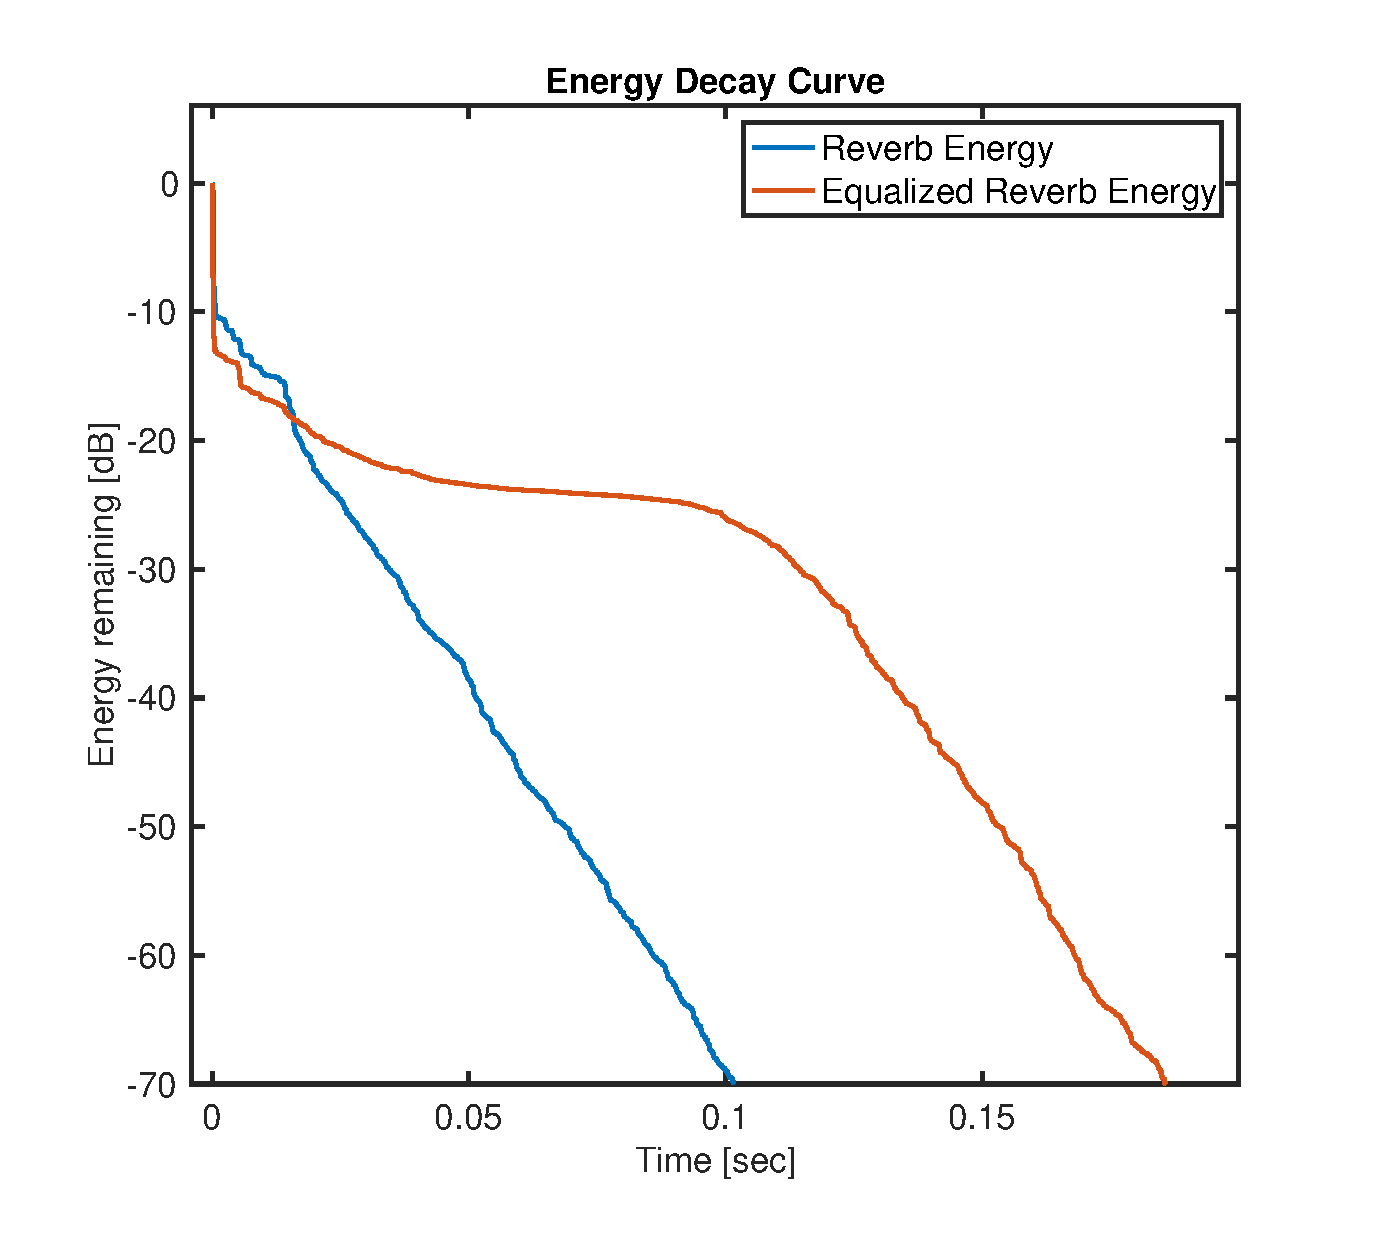
\includegraphics[width=\linewidth]{EDC_SourceLength_1_Blind}
			\end{subfigure}
		\end{minipage}
	}
	% Dummy subfigure for referencing row A
	\refstepcounter{subfigure}
	\label{subfig:params_source_length_compare:A}
	
	\vspace{1em}
	
	% ROW B
	\makebox[\textwidth][l]{%
		\begin{minipage}{0.08\textwidth}
			\centering
			\raggedleft{\footnotesize \textbf{(b)} \newline \qty{7.3}{\sec} \newline source} \\
		\end{minipage}%
		\begin{minipage}{0.91\textwidth}
			\begin{subfigure}[t]{0.32\textwidth}
				\centering
				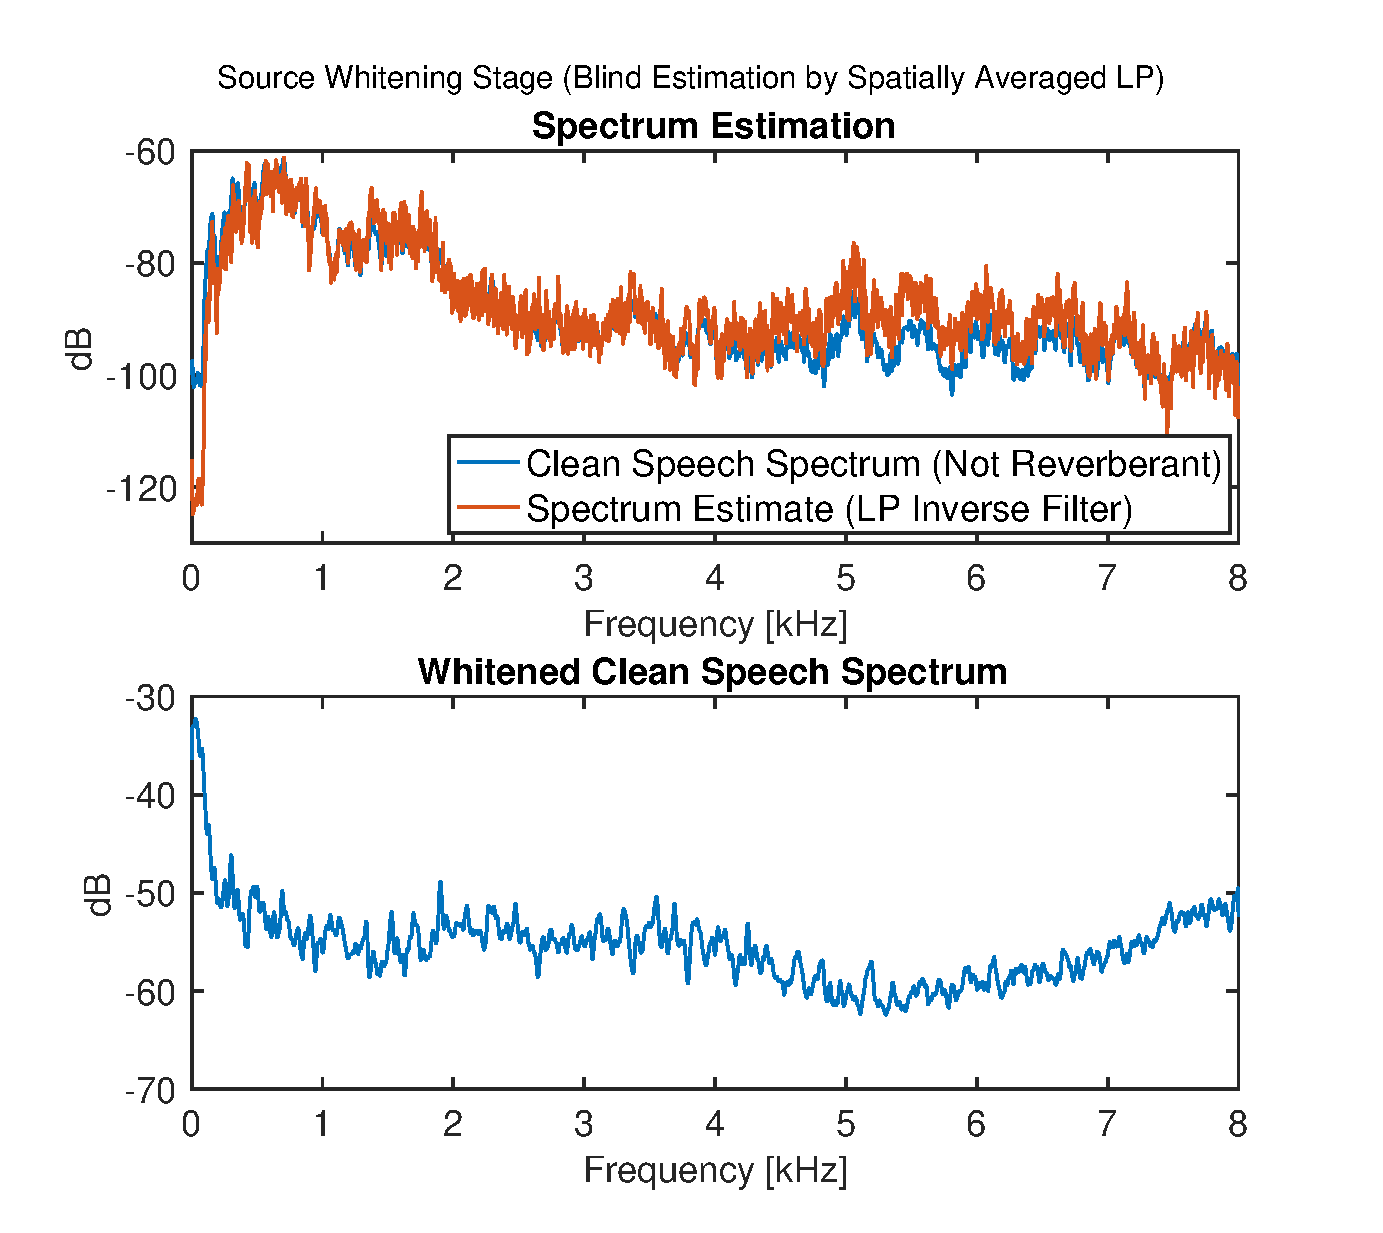
\includegraphics[width=\linewidth]{S1_SourceLength_2_Blind}
			\end{subfigure}
			\hfill
			\begin{subfigure}[t]{0.32\textwidth}
				\centering
				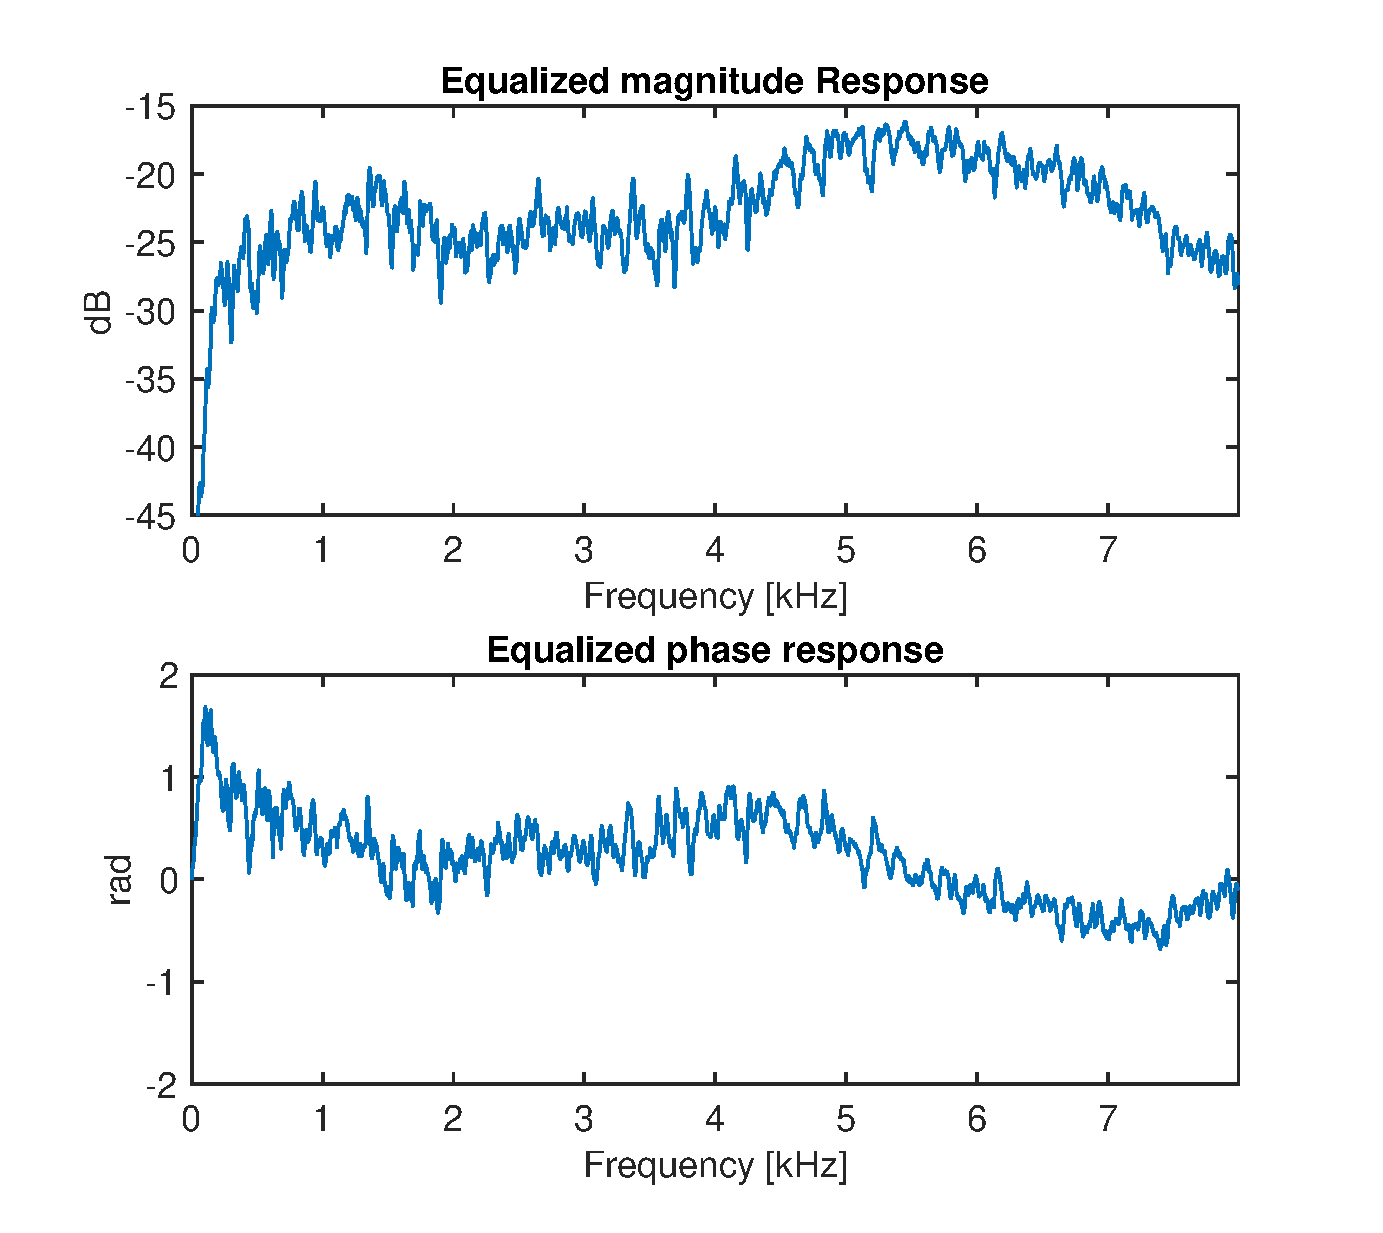
\includegraphics[width=\linewidth]{Equalized_RTF_SourceLength_2_Blind}
			\end{subfigure}
			\hfill
			\begin{subfigure}[t]{0.32\textwidth}
				\centering
				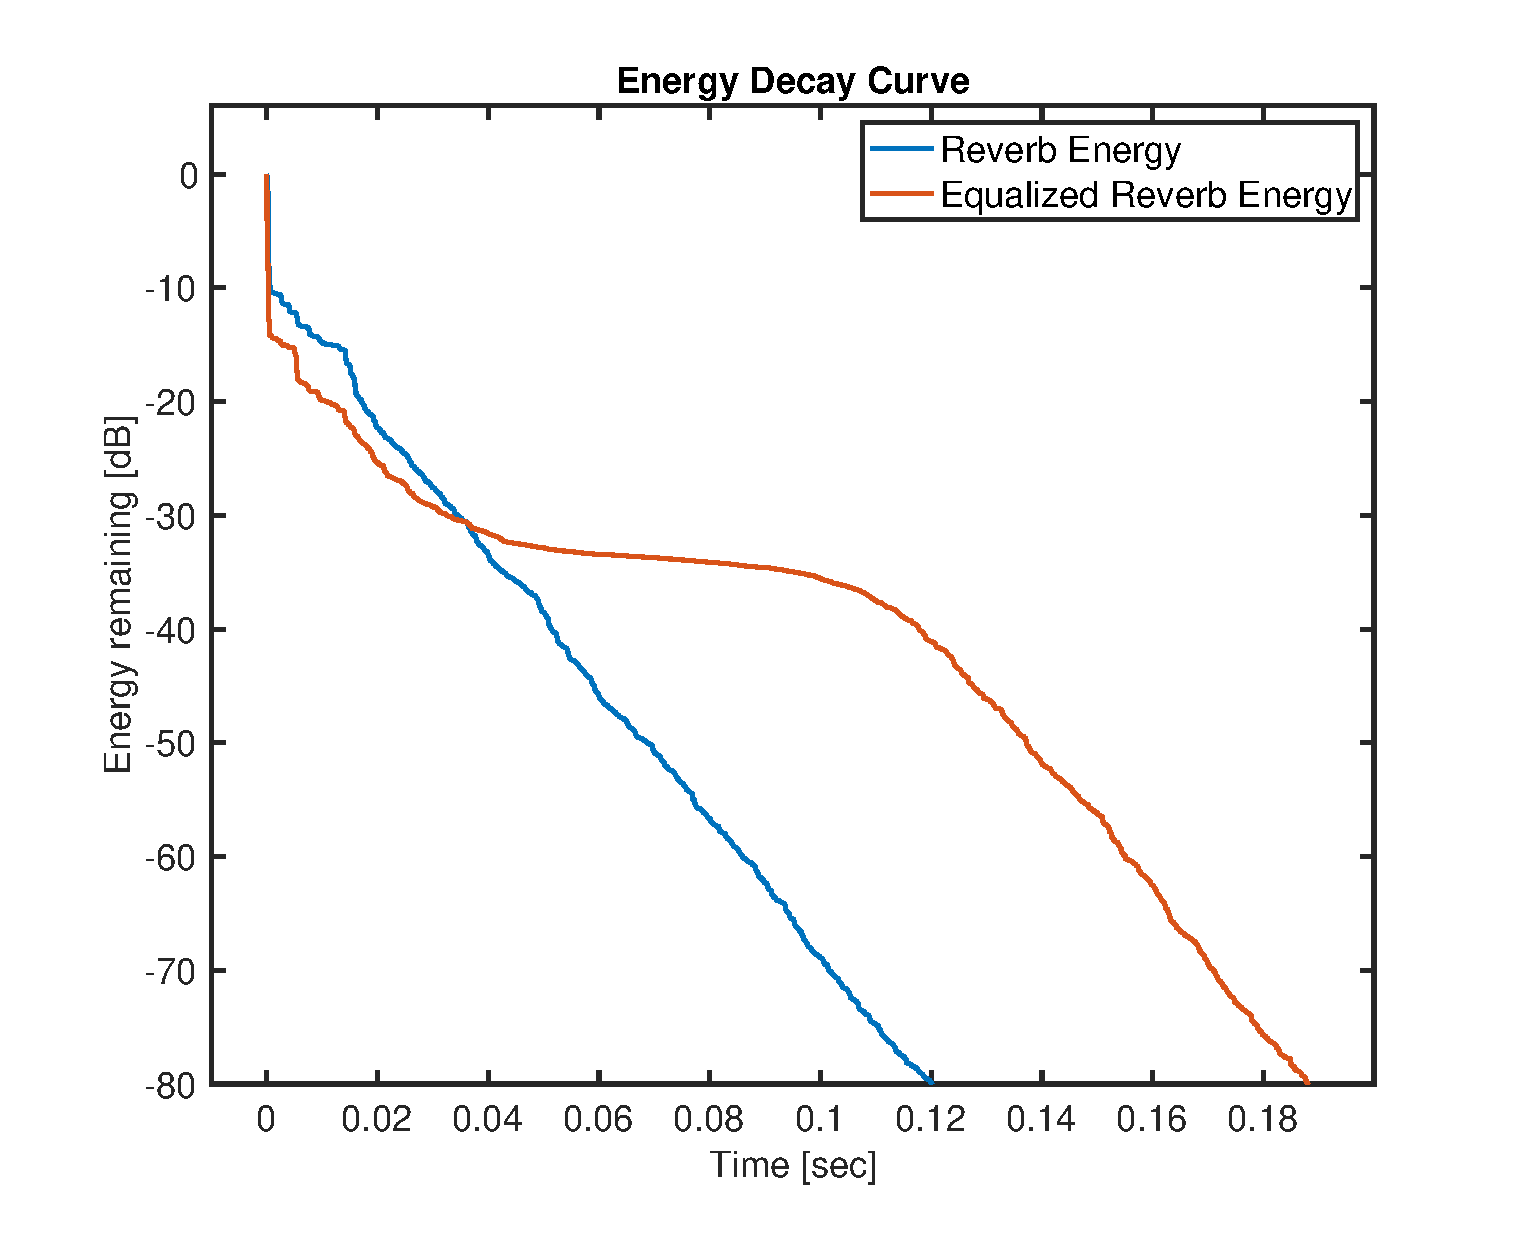
\includegraphics[width=\linewidth]{EDC_SourceLength_2_Blind}
			\end{subfigure}
		\end{minipage}
	}
	% Dummy subfigure for referencing row B
	\refstepcounter{subfigure}
	\label{subfig:params_source_length_compare:B}
	
	\vspace{1em}
	
	% ROW C
	\makebox[\textwidth][l]{%
		\begin{minipage}{0.08\textwidth}
			\centering
			\raggedleft{\footnotesize \textbf{(c)} \newline \qty{10.9}{\sec} \newline source} \\
		\end{minipage}%
		\begin{minipage}{0.91\textwidth}
			\begin{subfigure}[t]{0.32\textwidth}
				\centering
				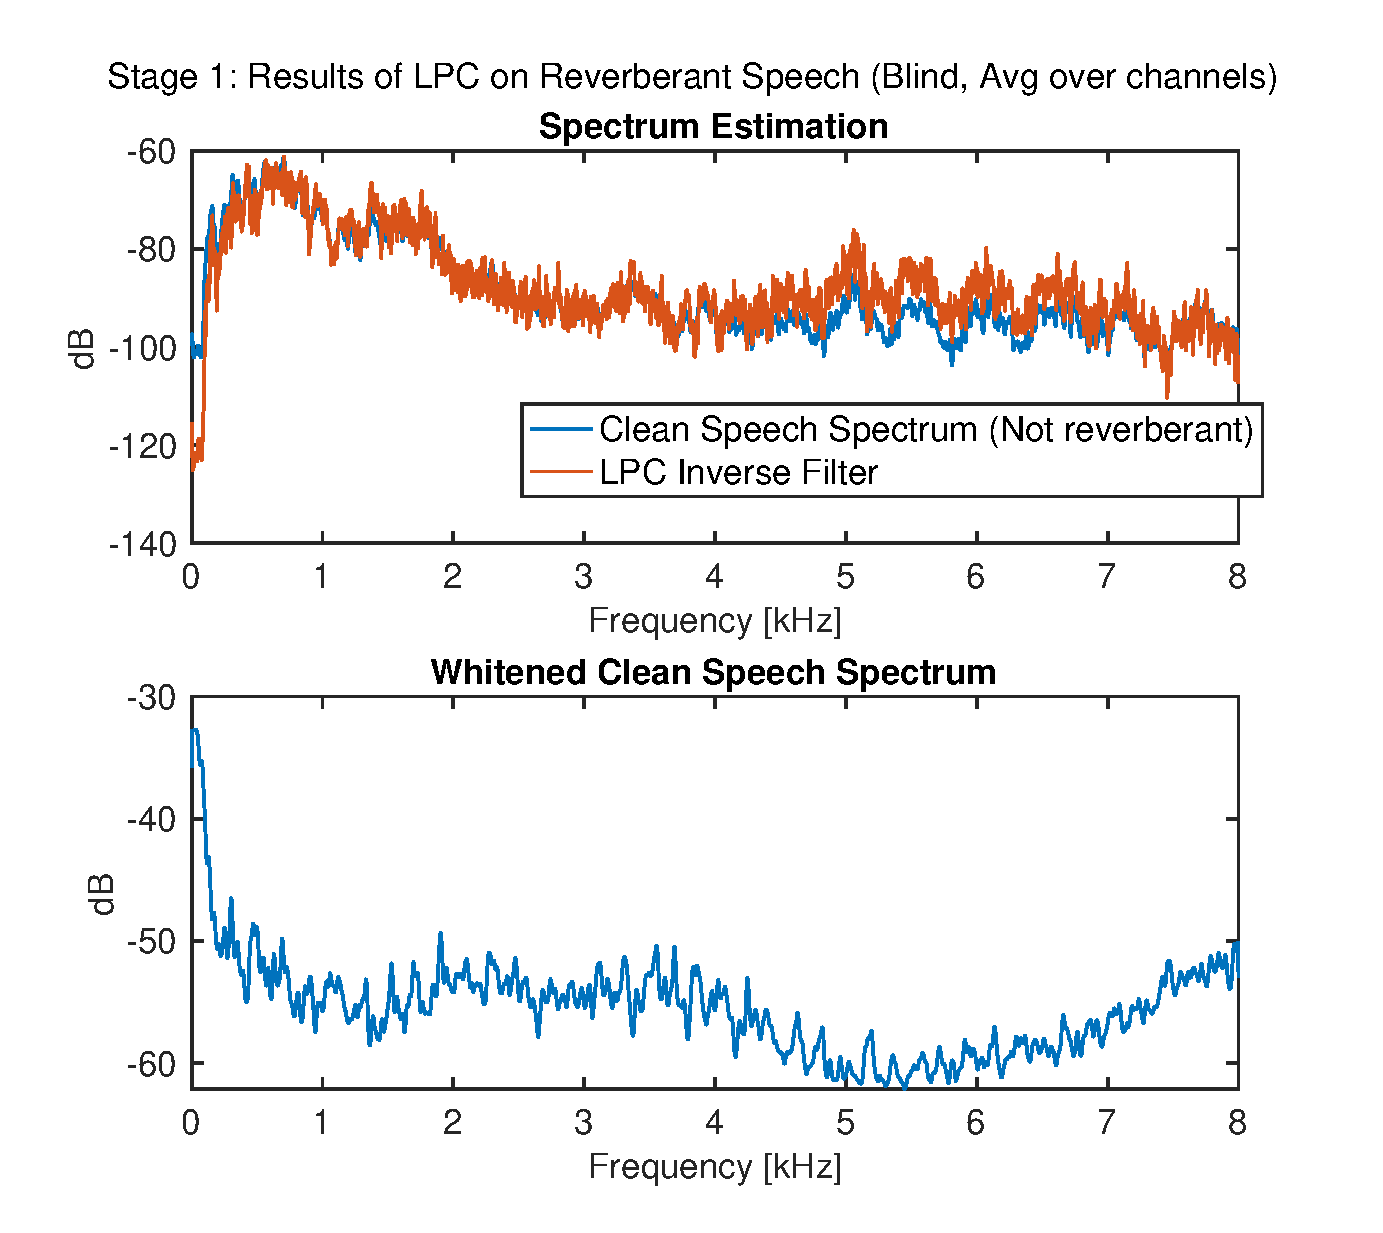
\includegraphics[width=\linewidth]{S1_SourceLength_3_Blind}
			\end{subfigure}
			\hfill
			\begin{subfigure}[t]{0.32\textwidth}
				\centering
				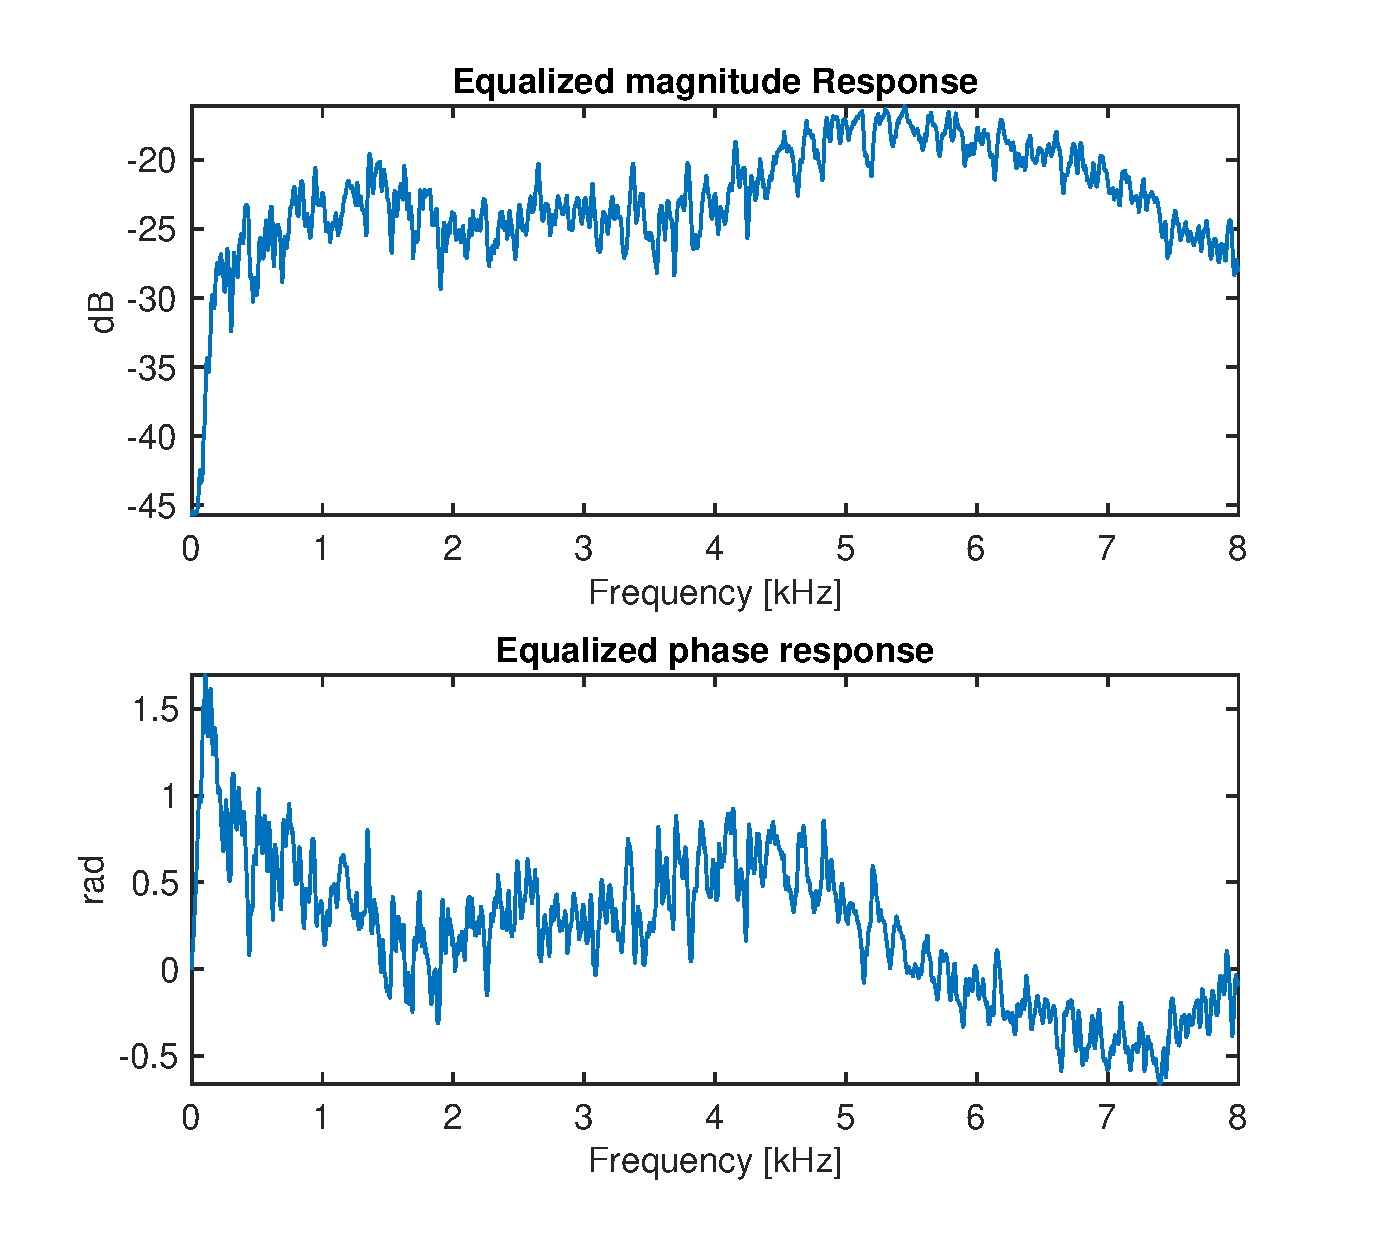
\includegraphics[width=\linewidth]{Equalized_RTF_SourceLength_3_Blind}
			\end{subfigure}
			\hfill
			\begin{subfigure}[t]{0.32\textwidth}
				\centering
				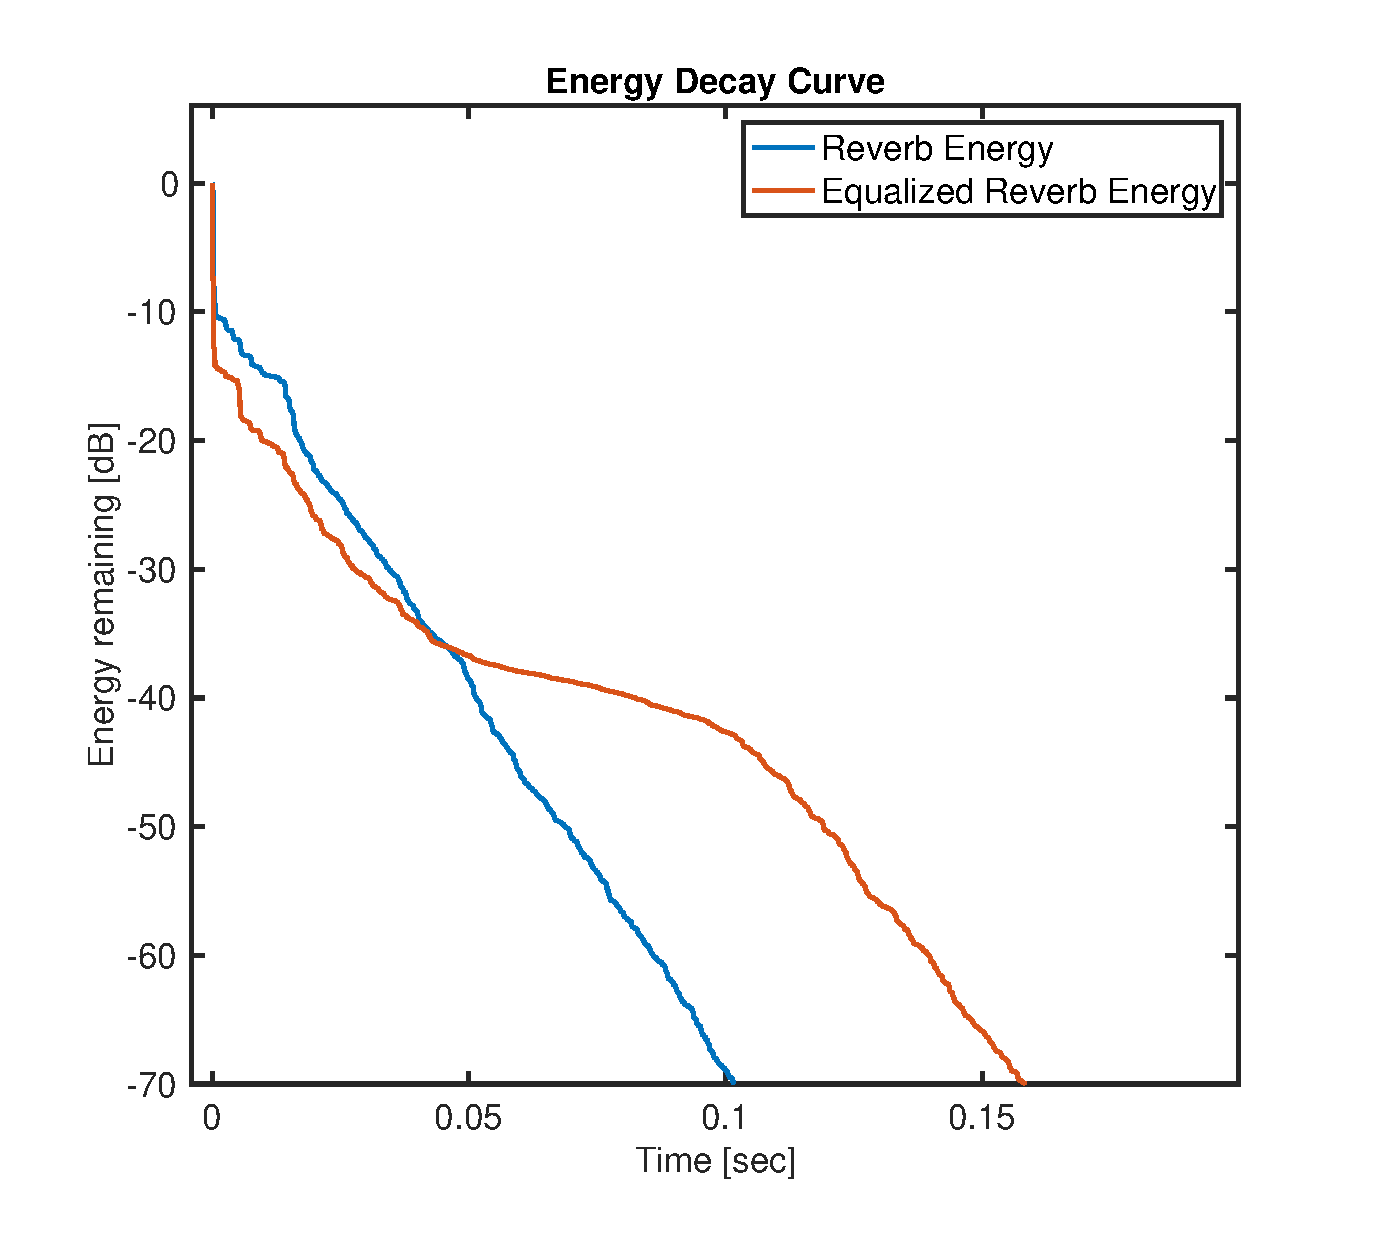
\includegraphics[width=\linewidth]{EDC_SourceLength_3_Blind}
			\end{subfigure}
		\end{minipage}
	}
	% Dummy subfigure for referencing row C
	\refstepcounter{subfigure}
	\label{subfig:params_source_length_compare:C}
	
	\vspace{1em}
	
	% ROW D
	\makebox[\textwidth][l]{%
		\begin{minipage}{0.08\textwidth}
			\centering
			\raggedleft{\footnotesize \textbf{(d)} \newline \qty{14.5}{\sec} \newline source} \\
		\end{minipage}%
		\begin{minipage}{0.91\textwidth}
			\begin{subfigure}[t]{0.32\textwidth}
				\centering
				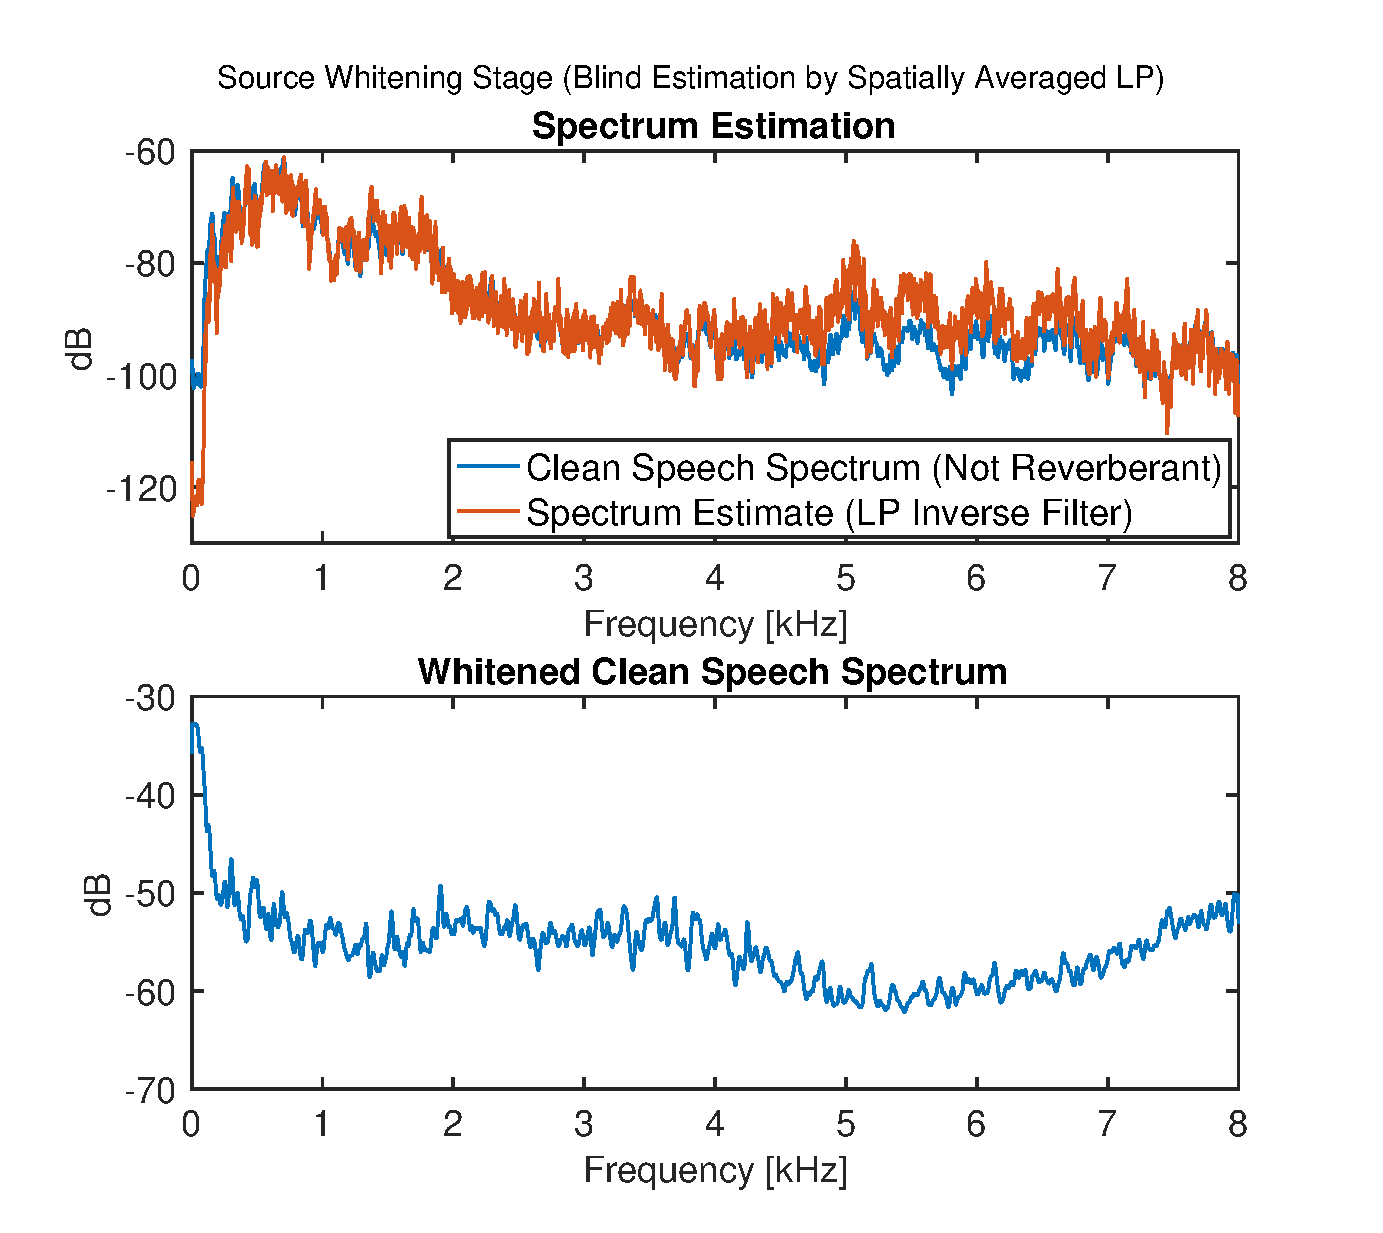
\includegraphics[width=\linewidth]{S1_SourceLength_4_Blind}
			\end{subfigure}
			\hfill
			\begin{subfigure}[t]{0.32\textwidth}
				\centering
				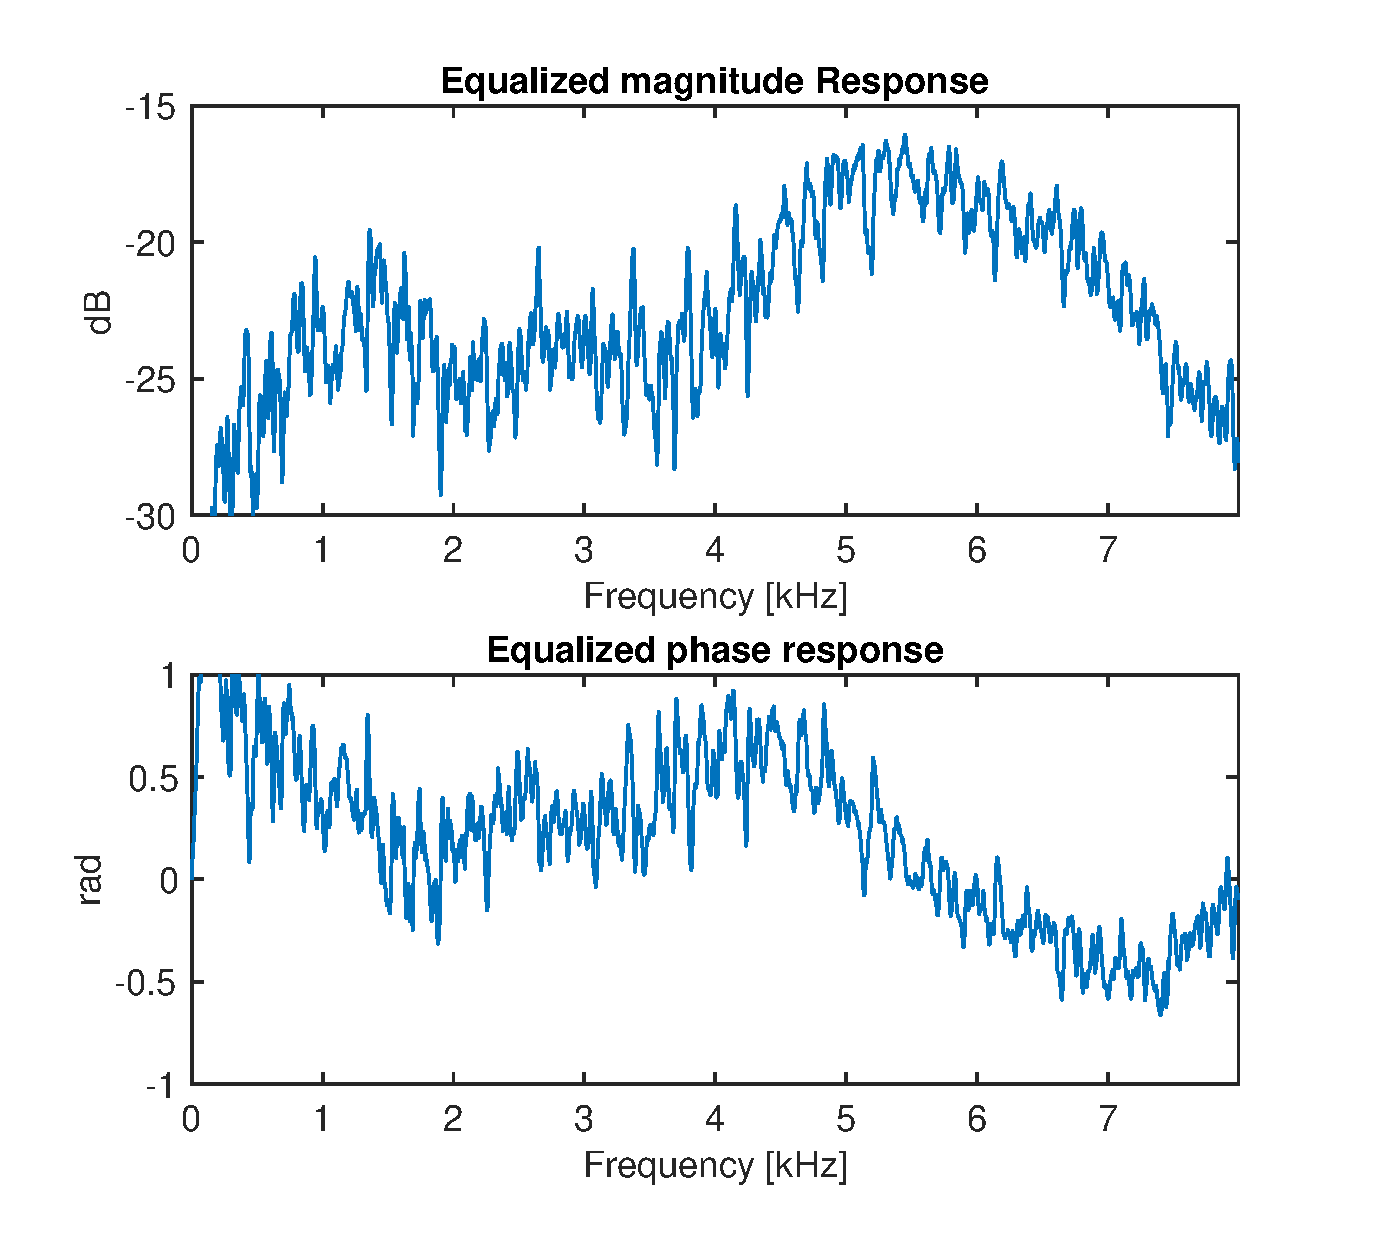
\includegraphics[width=\linewidth]{Equalized_RTF_SourceLength_4_Blind}
			\end{subfigure}
			\hfill
			\begin{subfigure}[t]{0.32\textwidth}
				\centering
				\includegraphics[width=\linewidth]{EDC_SourceLength_4_Blind}
			\end{subfigure}
		\end{minipage}
	}
	% Dummy subfigure for referencing row D
	\refstepcounter{subfigure}
	\label{subfig:params_source_length_compare:D}
	
	\caption{Delay-and-Predict dereverberation performance with the same speech sample (SA1.WAV, \qty{3.6}{\sec}, or \qty{58}{\kilo samples}) looped to various data lengths to preserve the same spectrum. Source whitening prediction order was $\mathrm{p1} = 2 \cdot \mathrm{p2} \cdot (M-1)$ and multichannel linear prediction order was $\mathrm{p2} = \mathrm{N60} / (M-1)$. Source Whitening stage was performed on revererbant speech (i.e., blind).}
	\label{fig:params_source_length_compare}
	
\end{figure}

Comparing the EDC results (third column in Figure \ref{fig:params_source_length_compare}), it is clear that the amount of source data used in training the algorithm has an impact on reverberation cancellation performance, independent of the source spectrum. Specifically, it was observed that the level at which the EDC plateaus (i.e., the point at which estimation variance is strong relative to reverberation as previously discussed) scales approximately from \qty{20}{\decibel} in Figure \ref{subfig:params_source_length_compare:A} to \qty{35}{\decibel} in Figure \ref{subfig:params_source_length_compare:D}. Or viewed differently, the percentage of the full RIR T60 that the algorithm was able to provide any attenuation of the RIR was observed to scale approximately from $\qty{25}{\milli\sec} / \qty{100}{\milli\sec}=25 \%$ to $\qty{50}{\milli\sec} / \qty{100}{\milli\sec}=50 \%$. The dependency of performance on the amount of source data used in training makes sense because as the prediction order increases, estimation variance of the longer lag autocorrelation values increases, thus requiring more data to bring it down to a reasonable level. Converesely, linear prediction in the context of traditional speech coding uses lower orders (often modeling as few as 8-16 poles), thus requiring far less data to minimize estimation variance. In speech coding, the goal is often to model only the more prominent spectral shape (i.e., more of a spectral envelope) and the smaller spectral details may be neglected. In dereverberation, the final details of the RTF, which are the frequency-dual of the later/weaker part of the RIR, are non-negligible as they contribute to the perceptual reverberance of the room. 

Interestingly the increased estimation variance for smaller training signal lengths was only found to be visible in the source-whitening results and equalized RTF results (columns 1 and 2) in the first test case, i.e., Figure \ref{subfig:params_source_length_compare:A}. The variance is visible in this case as substantial ripples and deviation in the whitened clean speech spectrum, equalized magnitude response and equalized phase response. For larger training signal lengths, the difference in these plots were found to be less obvious, but the benefit was still visible in the EDC results as explained above.

The EDC benefit of increasing the amount of source data was observed to hit a ceiling over about \qty{10}{\sec} of data (i.e., over approximately \qty{160}{\kilo samples}), which is highly dependent on the specific prediction orders used in this test. If the prediction orders were increased, more data would be needed to acheive the same performance. Therefore, the amount of data used in training the algorithm (i.e., used in the normal equations) should be selected as needed to minimize estimation variance for the selected prediction orders. However, in practice the amount of data used is limited by the time-varying nature of RTFs. An analysis window of \qty{10}{\sec} of data was used for the remainer of this thesis, since anything larger would be completely unreasonble to assume a stationary RTF. The massive amount of data needed severely impacts the ability of MC-LP approaches to reverberation cancellation to track time-varying acoustics.

\subsection{Source Spectrum}

To evaluate the impact of source spectrum, in each test case the source was produced by synthetically generating a random white noise sequence of a different length (\qty{100}{\milli\sec}, \qty{1}{\sec} and \qty{10}{\sec} respectively), then looping these sequences to the same length (a duration of \qty{60}{\sec}). Since shorter realizations of the same uncorrelated (white) random process have a higher degree of correlation, this results in \qty{60}{\sec} sequences with controllable spectral peakiness. The results for each case are shown in Figure \ref{fig:params_source_spectrum_compare}. The same 4-channel RIR, and prediction orders were used as in the last section.

% Test: Same length different spectrum
% -     Blind DAP
% - 	Test: Speech is different length white noise sequences looped to length = 60 sec = 960000 (as original sequence length goes down, peakiness of spectrum goes up but final length doesn’t change)
% - 	RIR = SAL truncated to 100 msec = 1600 samples, M = 4 mics
% - 	P1 = 2 * p2 * (M-1)
% - 	P2 = N60 / (M-1)

% Source Spectrum Compare, Initial White noise sequence length = [0.1 sec 1 sec  10 sec], Blind
\begin{figure}[H]
	\centering
	
	% ROW A
	\makebox[\textwidth][l]{%
		\begin{minipage}{0.07\textwidth}
			\centering
			\raggedleft{\footnotesize \textbf{(a)} \newline \qty{0.1}{\sec} \newline white \newline noise} \\
		\end{minipage}%
		\begin{minipage}{0.92\textwidth}
			\begin{subfigure}[t]{0.32\textwidth}
				\centering
				\includegraphics[width=\linewidth]{S1_SourceSpectrum_100msecWhiteNoise_Blind}
			\end{subfigure}
			\hfill
			\begin{subfigure}[t]{0.32\textwidth}
				\centering
				\includegraphics[width=\linewidth]{Equalized_RTF_SourceSpectrum_100msecWhiteNoise_Blind}
			\end{subfigure}
			\hfill
			\begin{subfigure}[t]{0.32\textwidth}
				\centering
				\includegraphics[width=\linewidth]{EDC_SourceSpectrum_100msecWhiteNoise_Blind}
			\end{subfigure}
		\end{minipage}
	}
	% Dummy subfigure for referencing row A
	\refstepcounter{subfigure}
	\label{subfig:params_source_spectrum_compare:A}
	
	\vspace{1em}
	
	% ROW B
	\makebox[\textwidth][l]{%
		\begin{minipage}{0.07\textwidth}
			\centering
			\raggedleft{\footnotesize \textbf{(b)} \newline \qty{1}{\sec} \newline white \newline noise} \\
		\end{minipage}%
		\begin{minipage}{0.92\textwidth}
			\begin{subfigure}[t]{0.32\textwidth}
				\centering
				\includegraphics[width=\linewidth]{S1_SourceSpectrum_1secWhiteNoise_Blind}
			\end{subfigure}
			\hfill
			\begin{subfigure}[t]{0.32\textwidth}
				\centering
				\includegraphics[width=\linewidth]{Equalized_RTF_SourceSpectrum_1secWhiteNoise_Blind}
			\end{subfigure}
			\hfill
			\begin{subfigure}[t]{0.32\textwidth}
				\centering
				\includegraphics[width=\linewidth]{EDC_SourceSpectrum_1secWhiteNoise_Blind}
			\end{subfigure}
		\end{minipage}
	}
	% Dummy subfigure for referencing row B
	\refstepcounter{subfigure}
	\label{subfig:params_source_spectrum_compare:B}
	
	\vspace{1em}
	
	% ROW C
	\makebox[\textwidth][l]{%
		\begin{minipage}{0.07\textwidth}
			\centering
			\raggedleft{\footnotesize \textbf{(c)} \newline \qty{10}{\sec} \newline white \newline noise} \\
		\end{minipage}%
		\begin{minipage}{0.92\textwidth}
			\begin{subfigure}[t]{0.32\textwidth}
				\centering
				\includegraphics[width=\linewidth]{S1_SourceSpectrum_10secWhiteNoise_Blind}
			\end{subfigure}
			\hfill
			\begin{subfigure}[t]{0.32\textwidth}
				\centering
				\includegraphics[width=\linewidth]{Equalized_RTF_SourceSpectrum_10secWhiteNoise_Blind}
			\end{subfigure}
			\hfill
			\begin{subfigure}[t]{0.32\textwidth}
				\centering
				\includegraphics[width=\linewidth]{EDC_SourceSpectrum_10secWhiteNoise_Blind}
			\end{subfigure}
		\end{minipage}
	}
	% Dummy subfigure for referencing row C
	\refstepcounter{subfigure}
	\label{subfig:params_source_spectrum_compare:C}
	
	\caption{Delay-and-Predict dereverberation performance with the source signal generated by looping various length white noise sequences synthetically looped the \qty{60}{\sec} (i.e., same data length, different spectra). Source whitening prediction order was $\mathrm{p1} = 2 \cdot \mathrm{p2} \cdot (M-1)$ and multichannel linear prediction order was $\mathrm{p2} = \mathrm{N60} / (M-1)$. Source Whitening stage was performed on revererbant speech (i.e., blind).}
	\label{fig:params_source_spectrum_compare}
	
\end{figure}

As expected, reverberation cancellation performance scales with how uncorrelated (i.e., white) the source signal. As previously mentioned, this can potentially be attributed to the inverse proportionality between the conditioning of the normal equations and the spectral dynamic range of source signal (i.e., spectral envelope), and to the demand on the source-whitening stage as the source spectrum becomes more detailed (i.e., fine details of spectrum). To distinguish between these two explanations, an additional test was conducted whereby the source signals were generated by filtering the same white noise sequence with filters of varying peakiness. In this way, the fine details of the source spectrum are the same between tests, but the spectral dynamic range is varied.

% Source Spectrum Compare, Same 60 sec white noise sequence shaped with 3 filters of varying peakiness.
\begin{figure}[H]
	\centering
	
	% ROW A
	\makebox[\textwidth][l]{%
		\begin{minipage}{0.08\textwidth}
			\centering
			\raggedleft{\footnotesize \textbf{(a)} \newline Filter 1} \\
		\end{minipage}%
		\begin{minipage}{0.91\textwidth}
			\begin{subfigure}[t]{0.32\textwidth}
				\centering
				\includegraphics[width=\linewidth]{S1_SourceSpectrum_10secShapedNoise_filter1_Blind}
			\end{subfigure}
			\hfill
			\begin{subfigure}[t]{0.32\textwidth}
				\centering
				\includegraphics[width=\linewidth]{Equalized_RTF_SourceSpectrum_10secShapedNoise_filter1_Blind}
			\end{subfigure}
			\hfill
			\begin{subfigure}[t]{0.32\textwidth}
				\centering
				\includegraphics[width=\linewidth]{EDC_SourceSpectrum_10secShapedNoise_filter1_Blind}
			\end{subfigure}
		\end{minipage}
	}
	% Dummy subfigure for referencing row A
	\refstepcounter{subfigure}
	\label{subfig:params_source_spectrum_shaped_compare:A}
	
	\vspace{1em}
	
	% ROW B
	\makebox[\textwidth][l]{%
		\begin{minipage}{0.08\textwidth}
			\centering
			\raggedleft{\footnotesize \textbf{(b)} \newline Filter 2} \\
		\end{minipage}%
		\begin{minipage}{0.91\textwidth}
			\begin{subfigure}[t]{0.32\textwidth}
				\centering
				\includegraphics[width=\linewidth]{S1_SourceSpectrum_10secShapedNoise_filter2_Blind}
			\end{subfigure}
			\hfill
			\begin{subfigure}[t]{0.32\textwidth}
				\centering
				\includegraphics[width=\linewidth]{Equalized_RTF_SourceSpectrum_10secShapedNoise_filter2_Blind}
			\end{subfigure}
			\hfill
			\begin{subfigure}[t]{0.32\textwidth}
				\centering
				\includegraphics[width=\linewidth]{EDC_SourceSpectrum_10secShapedNoise_filter2_Blind}
			\end{subfigure}
		\end{minipage}
	}
	% Dummy subfigure for referencing row B
	\refstepcounter{subfigure}
	\label{subfig:params_source_spectrum_shaped_compare:B}
	
	\vspace{1em}
	
	% ROW C
	\makebox[\textwidth][l]{%
		\begin{minipage}{0.08\textwidth}
			\centering
			\raggedleft{\footnotesize \textbf{(c)} \newline Filter 3} \\
		\end{minipage}%
		\begin{minipage}{0.91\textwidth}
			\begin{subfigure}[t]{0.32\textwidth}
				\centering
				\includegraphics[width=\linewidth]{S1_SourceSpectrum_10secShapedNoise_filter3_Blind}
			\end{subfigure}
			\hfill
			\begin{subfigure}[t]{0.32\textwidth}
				\centering
				\includegraphics[width=\linewidth]{Equalized_RTF_SourceSpectrum_10secShapedNoise_filter3_Blind}
			\end{subfigure}
			\hfill
			\begin{subfigure}[t]{0.32\textwidth}
				\centering
				\includegraphics[width=\linewidth]{EDC_SourceSpectrum_10secShapedNoise_filter3_Blind}
			\end{subfigure}
		\end{minipage}
	}
	% Dummy subfigure for referencing row C
	\refstepcounter{subfigure}
	\label{subfig:params_source_spectrum_shaped_compare:C}
	
	\caption{Delay-and-Predict dereverberation performance with the source signal generated by filtering \qty{60}{\milli\sec} of speech with filters of various peakiness. Source whitening prediction order was $\mathrm{p1} = 2 \cdot \mathrm{p2} \cdot (M-1)$ and multichannel linear prediction order was $\mathrm{p2} = \mathrm{N60} / (M-1)$. Source Whitening stage was performed on revererbant speech (i.e., blind).}
	\label{fig:params_source_spectrum_shaped_compare}
	
\end{figure}

As shown in Figure \ref{fig:params_source_spectrum_shaped_compare}, the spectral dynamic range alone has very minimal impact on performance. This makes sense because the normal equations are constructed using the reverberant microphone signals, not the clean speech. RTFs are known to have strong notches and resonances, thus reverberant signals tend to have a large spectral dynamic range irrespective of the source signal spectrum. Thus it was concluded that the primary spectral characteristic of the source signal that impacts performance is the complexity of fine spectral details, which make the job of the source-whitening stage more difficult.


\section{Time Alignment of RIRs and Linear Combiner}

To evaluate the influence of time alignment of the RIRs on dereverberation performance, the DAP algorithm was run excluding the diagonal delay matrix, $\boldsymbol{D}(z)$. The four RIRs were generated synthetically by applying an exponentially decaying window to a Gaussian white noise sequence and then were maually delayed to misalign them. Figure \ref{fig:params_MC_EIR_TimeAlignment_0sampleDelay} shows the results when the RIRs are time aligned, and Figure \ref{fig:params_MC_EIR_TimeAlignment_2sampleDelay} shows the results when an incremental delay of two samples was introduced accross the microphones. The delay increases from channel 1 to channel 4, i.e., channel 1 leads all other channels. The left column of the results plots shows RIR for each channel. The right column shows the four EIRs prior to linear combination, i.e., the vector-valued EIR excluding the linear combiner vector, $\boldsymbol{\mathrm{eir}}(z) = \begin{bmatrix} \mathrm{eir}_1 (z)& \dots & \mathrm{eir}_M(z) \end{bmatrix}^T$. 

\begin{equation}
	\boldsymbol{\mathrm{eir}}(z) = \boldsymbol{g}(z)\boldsymbol{A}_{pe,mc}(z)
\end{equation}

\noindent
where $\boldsymbol{g}(z) = \begin{bmatrix} G_1(z)& \dots & G_M(z) \end{bmatrix}^T$ is the vector-valued $M$-channel RTF.

%Test:
% - Synthetic RIRs, delayed manually (incremental delay added per channel), T60=100msec
% - L channel = N60 * 2 = 3200 samples (~120 dB attenuation)
% - Source = SA1.wav looped for 20 sec
% - S1 on clean speech
% - Figures saved (.fig)


\begin{figure}[H]
	\includegraphics[width=0.8\textwidth]{MC_EIR_TimeAlignment_0sampleDelay}
	\centering
	\caption{Vector-valued EIR performance prior to linear combiner with no time delay between channels (i.e., time aligned).}
	\label{fig:params_MC_EIR_TimeAlignment_0sampleDelay}
\end{figure}

\begin{figure}[H]
	\includegraphics[width=0.8\textwidth]{MC_EIR_TimeAlignment_2sampleDelay}
	\centering
	\caption{Vector-valued EIR performance prior to linear combiner with an incremental 2-sample delay added to each channel (i.e., not time aligned).}
	\label{fig:params_MC_EIR_TimeAlignment_2sampleDelay}
\end{figure}


From Figure \ref{fig:params_MC_EIR_TimeAlignment_0sampleDelay}, note that all four individual EIRs show an impulse-like shape, suggesting reasonable equalization. However, in Figure \ref{fig:params_MC_EIR_TimeAlignment_2sampleDelay}, it was observed that whenever the signal being predicted by the MC-LP stage leads the other signals, the signal is eliminated instead of the channel being equalized (i.e., the EIR is all zeros instead of becoming impulse-like). This is an expected behavior of MC-LP since the whitening nature of linear prediction is due to the signal only being estimated strictly from past samples. If channel 2 lags channel 1 by samples, prediction of channel 2 from channel 1 will have access to current source information, thus being able to perfectly cancel it instead of only whitening. Additionally, when predicting the channel that leads the rest (thus remaining a whitening process), the lack of time alignment still negatively impacts performance, which is evident from the burst of unequalized reverberation in the row 1 EIR from Figure \ref{fig:params_MC_EIR_TimeAlignment_2sampleDelay}. Time alignment has a clear impact on dereverberation performance after linear combination as well, as shown in Figure \ref{fig:params_TimeAlignment_0sampleDelay} and Figure \ref{fig:params_TimeAlignment_2sampleDelay} below.


\begin{figure}[H]
	\centering
	\begin{subfigure}[b]{0.32\textwidth}
		\centering
		\includegraphics[width=\textwidth]{EIR_TimeAlignment_0sampleDelay}
	\end{subfigure}
	\hfill
	\begin{subfigure}[b]{0.32\textwidth}
		\centering
		\includegraphics[width=\textwidth]{Equalized_RTF_TimeAlignment_0sampleDelay}
	\end{subfigure}
	\hfill
	\begin{subfigure}[b]{0.32\textwidth}
		\centering
		\includegraphics[width=\textwidth]{EDC_TimeAlignment_0sampleDelay}
	\end{subfigure}
	\hfill
	\caption{Delay-and-Predict dereverberation performance (after linear combiner) with an incremental 2-sample delay added to each channel (i.e., not time aligned).}
	\label{fig:params_TimeAlignment_0sampleDelay}
\end{figure}

\begin{figure}[H]
	\centering
	\begin{subfigure}[b]{0.32\textwidth}
		\centering
		\includegraphics[width=\textwidth]{EIR_TimeAlignment_2sampleDelay}
	\end{subfigure}
	\hfill
	\begin{subfigure}[b]{0.32\textwidth}
		\centering
		\includegraphics[width=\textwidth]{Equalized_RTF_TimeAlignment_2sampleDelay}
	\end{subfigure}
	\hfill
	\begin{subfigure}[b]{0.32\textwidth}
		\centering
		\includegraphics[width=\textwidth]{EDC_TimeAlignment_2sampleDelay}
	\end{subfigure}
	\hfill
	\caption{Delay-and-Predict dereverberation performance (after linear combiner) with no time delay between channels (i.e., time aligned)}
	\label{fig:params_TimeAlignment_2sampleDelay}
\end{figure}

The linear combiner used ($\boldsymbol{g}_0$) was the estimate of the first vector coefficient of the SIMO channel, as proposed by \cite{triki2006delay} and as discussed in Section \ref{section_dap}. From this analysis the motivation for using this linear combiner is evident: a larger value from $\boldsymbol{g}_0$ implies that the corresponding channel leads the others and as such will act as a whitening filter and not a signal cancellation filter, which is desired. Thus this linear combiner method puts larger weights on EIRs that are whitened (as desired) and therefore provides some protection against non-time-aligned channels. For the remainder of this thesis, the RIRs were manually time aligned, but this linear combination method was still used.

\section{Algorithmic Complexity Analysis}

An important consideration in selecting the linear prediction orders for the source-whitening and MC-LP stages is the memory and computational requirements required to implement the algorithm. Figure \ref{fig:complexity_operations} and Figure \ref{fig:complexity_memory} show required mathematical operations and memory scale with these parameters. The x-axis for these plots is T60, and the prediction orders used for each T60 are given by $p_2 = 0.75 \cdot N60 / \left(M-1\right)$ and $p_1 = 1.25 \cdot p_2 \cdot \left(M-1\right)$. These prediction orders were selected based on acheiving maximum performance for the given T60, as per the discussion in Section \ref{section:params_p2_MC_LP} and Section \ref{section:params_p1}. As such, the plots my be interpreted as showing the memory/computations required to provide maximum dereverberation performance for RIRs up to the given T60.

These plots were generated assuming $M=4$ microphones, a sample rate of \qty{16}{\kilo\hertz} and a 32 bits of numerical precision.

\begin{figure}[H]
	\centering
	\begin{subfigure}[b]{0.45\textwidth}
		\centering
		\includegraphics[width=\textwidth]{complexity_ops_comparison}
	\end{subfigure}
	\hfill
	\begin{subfigure}[b]{0.45\textwidth}
		\centering
		\includegraphics[width=\textwidth]{complexity_ops_comparison_zoomed}
	\end{subfigure}
	\caption{Analysis of the computational complexities of Least Squares solution and Inverse filter implementations as a function of T60, For $M=4$ microphones, $\mathrm{p2} = 0.75 \cdot \mathrm{N60}/(M-1)$ and $\mathrm{p1} = 1.25 \cdot \mathrm{p2} \cdot (M-1)$. Complexity of LMS Solution also shown for comparison.}
	\label{fig:complexity_operations}
\end{figure}

\begin{figure}[H]
	\centering
	\begin{subfigure}[b]{0.45\textwidth}
		\centering
		\includegraphics[width=\textwidth]{complexity_mem_comparison}
	\end{subfigure}
	\hfill
	\begin{subfigure}[b]{0.45\textwidth}
		\centering
		\includegraphics[width=\textwidth]{complexity_mem_comparison_zoomed}
	\end{subfigure}
	\caption{Analysis of the algorithmic memory requirements  of Least Squares solution (could be temporary memory) and Inverse filter implementations (persistent memory) as a function of T60, For M=4 microphones, $\mathrm{p2} = 0.75 \cdot \mathrm{N60}/(M-1)$ and $\mathrm{p1} = 1.25 \cdot \mathrm{p2} \cdot (M-1)$. Memory requirements of LMS Solution also shown for comparison.}
	\label{fig:complexity_memory}
\end{figure}

Both memory and computations associated with solving the normal equations scales exponentially with T60 up to which we wish to cancel. Equalizing RIRs up to a T60 of \qty{2}{\sec} requires approximately \qty{5e9}{operations} and  \qty{8}{\giga\byte} of memory, which is completely unrealistic in any practical system. Therefore for the purposes of the experiments in this thesis, it was decided to choose prediction orders to equalize RIRs up to a \qty{1}{\sec} T60, which requires approximately \qty{1e9}{operations} and \qty{2}{\giga\byte}. This may be realistic in systems with tremendous amounts of processing power and memory, but is still completely unrealistic in an embedded application such as a hearing aid. To implement the algorithm in a more constrained system, the prediction orders would have to be reduced signficantly. This is a severe limitation of the algorithm, and presents a motivation for the to enhance the algorithm with other reverberation suppression techniques in any practical system. Another approach to reduce algorithmic complexity would be to estimate the source-whitening and MC-LP filters using an adaptive algorithm such as LMS instead of directly solving the normal equations. Unlike the normal equations solution, LMS updates scale linearly with prediction order, only requiring approximately \qty{4.5e4}{operations} and \qty{250}{\kilo\byte} for $\mathrm{T60} = \qty{1}{\sec}$, which could be improved further by using frequency/subband-domain adaptation. Using an adaptive algorithm would of course come at a cost of worse performance, but could potentially do a better job of tracking time varying acoustics. This was left for a future study.


\section{Conclusions}

To summarize, a number of parameters of the DAP algorithm and signal properties were investigated in terms of their influence on dereverberation performance: 

\begin{enumerate}
	\item \textbf{Multichannel Linear Prediction Order} ($p_2$): While in theory, near-perfect equalization of a length-$L$ RIR is possible with $p_2 = L / \left(M-1\right)$, in practice no additional performance gain was found for approximately $p_2 > 0.75 \cdot \mathrm{N60} / \left(M-1\right)$. In particular it was noted that there was always an increase in residual reverberation towards the end of the RIR. This limitation was assumed to be due to autocorrelation estimation variance (especially at larger lags) due to limited signal data and the low energy of the late reflections. In practice it was found that the equalizer was only able to acheive up to approximately \qty{35}{\decibel} of reverberation suppression under ideal conditions. $p_2=\mathrm{N60}/\left(M-1\right)$ will be used for experiments in this thesis. 
	%
	\item \textbf{Source Whitening Linear Prediction Order} ($p_1$): It was found that it was important to set $p_1 > p_2 \cdot \left(M-1\right)$ to match the spectral resolution of the source-whitening filter to the "effective spectral resolution" of the MC-LP prediction error filter. $p_1 = 1.25 \cdot p_2 \cdot \left(M-1\right)$ was found to be reasonable.
	%
	\item \textbf{Source Data Length}: A significant amount of data was found to be needed to bring down the estimation variance of the larger autocorrelation lags. For a sample rate of \qty{16}{\kilo\hertz} and T60 of \qty{100}{\milli\sec} (with prediction orders set as above), no improvement was seen for over approximately \qty{10}{\sec} of data, but this is expected to scale somewhat with T60. However the amount of data used in training is limited by the time varying nature of RTFs. A training signal of \qty{10}{\sec} will be used for experiments in this thesis.
	%
	\item \textbf{Source Spectrum}: The spectrum of the source signal was found to have a strong influence on dereverberation performance. In particular it was found that the density of fine spectral details had a negative impact on performance. This was assumed to be due to the increased demand on the source-whitening stage and the challenge of blindly estimating a complex source spectrum by spatial autocorrelation averaging accross microphones.
	%
	\item \textbf{Time Alignment of RIRs}: The time-of-flight alignment of the RIRs (and therefore the resulting microphone signals) was found to be crucial to algorithm performance. Without aligning the RIRs, the basic formulation of linear prediction being the prediction of current signal samples from only past signal samples breaks down, and the prediction error filters become cancellation filters instead of whitening filters. For the purposes of this thesis, the RIRs will be manually time-aligned and this procedure was left for future studies.
	%
	\item \textbf{Linear Combine}r ($\boldsymbol{g}_0$): The linear combiner proposed by \cite{triki2006delay} was investaged and it was shown that this technique provides some protection against time-alignment issues. This linear combiner will be used for the remainder of this thesis.
\end{enumerate}

Additionally, the memory and computational requirements were investigated and found to severly limit the practical applicability of DAP dereverberation. For the experiments in this thesis, the MC-LP prediction order will therefore be set only to maximally cancel T60s up to \qty{1}{\sec} (i.e., $p_2=\mathrm{N60}/\left(M-1\right)$,  with $\mathrm{N60} = \mathrm{T60} \cdot \mathrm{sample \; rate}$, $\mathrm{T60} = \qty{1}{\sec}$).


\section{Appendices}

\subsection{MC-LP Order} \label{section:appendix:params_p2}

\textbf{p2 = L / (M-1)  (MINT based on RIR length)}

\begin{figure}[H]
	\centering
	\begin{subfigure}[b]{0.32\textwidth}
		\centering
		\includegraphics[width=\textwidth]{Equalized_RTF_L_div_M_minus_1}
		\subcaption{test} \label{subfig:test_subfig_1}
	\end{subfigure}
	\hfill
	\begin{subfigure}[b]{0.32\textwidth}
		\centering
		\includegraphics[width=\textwidth]{EIR_L_div_M_minus_1}
	\end{subfigure}
	\hfill
	\begin{subfigure}[b]{0.32\textwidth}
		\centering
		\includegraphics[width=\textwidth]{EDC_L_div_M_minus_1}
	\end{subfigure}
	\hfill
	\caption{Delay-and-Predict dereverberation performance with multichannel linear prediction order $\mathrm{p2} = L / (M-1)$, where $L$ is the FIR RIR length and $M$ is the number of channels. Figure \ref{fig:params_p2_stage1} shows the common source whitening filter used.}
	\label{fig:params_p2_L}
\end{figure}

\textbf{p2 = N60 / (M-1)  (MINT based on T60)}

\begin{figure}[H]
	\centering
	%\begin{subfigure}[b]{0.49\textwidth}
	%	\centering
	%	\includegraphics[width=\textwidth]{S1_N60_div_M_minus_1}
	%\end{subfigure}
	%\hfill
	\begin{subfigure}[b]{0.32\textwidth}
		\centering
		\includegraphics[width=\textwidth]{Equalized_RTF_N60_div_M_minus_1}
	\end{subfigure}
	\hfill
	\begin{subfigure}[b]{0.32\textwidth}
		\centering
		\includegraphics[width=\textwidth]{EIR_N60_div_M_minus_1}
	\end{subfigure}
	\hfill
	\begin{subfigure}[b]{0.32\textwidth}
		\centering
		\includegraphics[width=\textwidth]{EDC_N60_div_M_minus_1}
	\end{subfigure}
	\hfill
	\caption{Delay-and-Predict dereverberation performance with multichannel linear prediction order $\mathrm{p2} = \mathrm{N60} / (M-1)$, where N60 is the number of samples corresponding to the T60 and $M$ is the number of channels (i.e., the MINT condition based on T60 rather than the FIR RIR length). Figure \ref{fig:params_p2_stage1} shows the common source whitening filter used.}
	\label{fig:params_p2_N60}
\end{figure}

\textbf{p2 = 0p75 * N60 / (M-1) (Suboptimal)}

\begin{figure}[H]
	\centering
	%\begin{subfigure}[b]{0.49\textwidth}
	%	\centering
	%	\includegraphics[width=\textwidth]{S1_0p75N60_div_M_minus_1}
	%\end{subfigure}
	%\hfill
	\begin{subfigure}[b]{0.32\textwidth}
		\centering
		\includegraphics[width=\textwidth]{Equalized_RTF_0p75N60_div_M_minus_1}
	\end{subfigure}
	\hfill
	\begin{subfigure}[b]{0.32\textwidth}
		\centering
		\includegraphics[width=\textwidth]{EIR_0p75N60_div_M_minus_1}
	\end{subfigure}
	\hfill
	\begin{subfigure}[b]{0.32\textwidth}
		\centering
		\includegraphics[width=\textwidth]{EDC_0p75N60_div_M_minus_1}
	\end{subfigure}
	\hfill
	\caption{Delay-and-Predict dereverberation performance with multichannel linear prediction order $\mathrm{p2} = 0.75 \cdot \mathrm{N60} / (M-1)$, where N60 is the number of samples corresponding to the T60 and $M$ is the number of channels (i.e., suboptimal with respect to the MINT condition based on T60 rather than the FIR RIR length). Figure \ref{fig:params_p2_stage1} shows the common source whitening filter used.}
	\label{fig:params_p2_0p75_N60}
\end{figure}

\textbf{p2 = 0.5 * N60 / (M-1) (More suboptimal)}

\begin{figure}[H]
	\centering
	%\begin{subfigure}[b]{0.49\textwidth}
	%	\centering
	%	\includegraphics[width=\textwidth]{S1_0p5N60_div_M_minus_1}
	%\end{subfigure}
	%\hfill
	\begin{subfigure}[b]{0.32\textwidth}
		\centering
		\includegraphics[width=\textwidth]{Equalized_RTF_0p5N60_div_M_minus_1}
	\end{subfigure}
	\hfill
	\begin{subfigure}[b]{0.32\textwidth}
		\centering
		\includegraphics[width=\textwidth]{EIR_0p5N60_div_M_minus_1}
	\end{subfigure}
	\hfill
	\begin{subfigure}[b]{0.32\textwidth}
		\centering
		\includegraphics[width=\textwidth]{EDC_0p5N60_div_M_minus_1}
	\end{subfigure}
	\hfill
	\caption{Delay-and-Predict dereverberation performance with multichannel linear prediction order $\mathrm{p2} = 0.5 \cdot \mathrm{N60} / (M-1)$, where N60 is the number of samples corresponding to the T60 and $M$ is the number of channels (i.e., More suboptimal with respect to the MINT condition based on T60 rather than the FIR RIR length). Figure \ref{fig:params_p2_stage1} shows the common source whitening filter used.}
	\label{fig:params_p2_0p5_N60}
\end{figure}

\subsection{Source Whitening Order} \label{section:appendix:params_p1}

\textbf{p1 = 200 (Original Paper)}

\begin{figure}[H]
	\centering
	\begin{subfigure}[b]{0.49\textwidth}
		\centering
		\includegraphics[width=\textwidth]{S1_p1_200}
	\end{subfigure}
	\hfill
	\begin{subfigure}[b]{0.49\textwidth}
		\centering
		\includegraphics[width=\textwidth]{Equalized_RTF_p1_200}
	\end{subfigure}
	\hfill
	\begin{subfigure}[b]{0.49\textwidth}
		\centering
		\includegraphics[width=\textwidth]{EIR_p1_200}
	\end{subfigure}
	\hfill
	\begin{subfigure}[b]{0.49\textwidth}
		\centering
		\includegraphics[width=\textwidth]{EDC_p1_200}
	\end{subfigure}
	\hfill
	\caption{Delay-and-Predict dereverberation performance with source whitening prediction order $\mathrm{p1} = 200$ and multichannel linear prediction order $\mathrm{p2} = \mathrm{N60}  / (M-1)$.}
	\label{fig:params_p1_200}
\end{figure}

\textbf{p1 = 1000}

\begin{figure}[H]
	\centering
	\begin{subfigure}[b]{0.49\textwidth}
		\centering
		\includegraphics[width=\textwidth]{S1_p1_1000}
	\end{subfigure}
	\hfill
	\begin{subfigure}[b]{0.49\textwidth}
		\centering
		\includegraphics[width=\textwidth]{Equalized_RTF_p1_1000}
	\end{subfigure}
	\hfill
	\begin{subfigure}[b]{0.49\textwidth}
		\centering
		\includegraphics[width=\textwidth]{EIR_p1_1000}
	\end{subfigure}
	\hfill
	\begin{subfigure}[b]{0.49\textwidth}
		\centering
		\includegraphics[width=\textwidth]{EDC_p1_1000}
	\end{subfigure}
	\hfill
	\caption{Delay-and-Predict dereverberation performance with source whitening prediction order $\mathrm{p1} = 1000$ and multichannel linear prediction order $\mathrm{p2} = \mathrm{N60} / (M-1)$.}
	\label{fig:params_p1_1000}
\end{figure}

\textbf{p1 = p2 * (M-1) (whitened on the same spectral resolution as the MC-LP equalizer)}

\begin{figure}[H]
	\centering
	\begin{subfigure}[b]{0.49\textwidth}
		\centering
		\includegraphics[width=\textwidth]{S1_p1_based_on_p2}
	\end{subfigure}
	\hfill
	\begin{subfigure}[b]{0.49\textwidth}
		\centering
		\includegraphics[width=\textwidth]{Equalized_RTF_p1_based_on_p2}
	\end{subfigure}
	\hfill
	\begin{subfigure}[b]{0.49\textwidth}
		\centering
		\includegraphics[width=\textwidth]{EIR_p1_based_on_p2}
	\end{subfigure}
	\hfill
	\begin{subfigure}[b]{0.49\textwidth}
		\centering
		\includegraphics[width=\textwidth]{EDC_p1_based_on_p2}
	\end{subfigure}
	\hfill
	\caption{Delay-and-Predict dereverberation performance with source whitening prediction order $\mathrm{p1} = \mathrm{p2} \cdot (M-1)$ and multichannel linear prediction order $\mathrm{p2} = \mathrm{N60} / (M-1)$. I.e., The source whitening filter order is the same as the effective MINT filter order.}
	\label{fig:params_p1_based_on_p2}
\end{figure}

\textbf{p1 = 2 * p2  * (M-1) (Extra headroom)}

\begin{figure}[H]
	\centering
	\begin{subfigure}[b]{0.49\textwidth}
		\centering
		\includegraphics[width=\textwidth]{S1_p1_2x_p2}
	\end{subfigure}
	\hfill
	\begin{subfigure}[b]{0.49\textwidth}
		\centering
		\includegraphics[width=\textwidth]{Equalized_RTF_p1_2x_p2}
	\end{subfigure}
	\hfill
	\begin{subfigure}[b]{0.49\textwidth}
		\centering
		\includegraphics[width=\textwidth]{EIR_p1_2x_p2}
	\end{subfigure}
	\hfill
	\begin{subfigure}[b]{0.49\textwidth}
		\centering
		\includegraphics[width=\textwidth]{EDC_p1_2x_p2}
	\end{subfigure}
	\hfill
	\caption{Delay-and-Predict dereverberation performance with source whitening prediction order $\mathrm{p1} = 2 \cdot \mathrm{p2} \cdot (M-1)$ and multichannel linear prediction order $\mathrm{p2} = \mathrm{N60} / (M-1)$. I.e., The source whitening filter order is twice the effective MINT filter order.}
	\label{fig:params_p1_2x_p2}
\end{figure}

... beyond about p1 = 1.25 * p2 * (M-1) EDC performance saturates at approximately -35 dB reverb attenuation.


        \setcounter{figure}{0}
        \setcounter{equation}{0}
        \setcounter{table}{0}



%\chapter{Conclusions and Future Work}

 %       \setcounter{figure}{0}
  %     \setcounter{equation}{0}
   %     \setcounter{table}{0}
        
 \chapter{Conclusions and Future Work}

        \setcounter{figure}{0}
        \setcounter{equation}{0}
        \setcounter{table}{0}


 \appendix
               % you can include your appendix if you have any!

\bibliographystyle{natbib}
\bibliography{references}        % your list of references

\label{NumDocumentPages}

\end{document}
% ********************************
